\documentclass[twoside]{book}

% Packages required by doxygen
\usepackage{fixltx2e}
\usepackage{calc}
\usepackage{doxygen}
\usepackage[export]{adjustbox} % also loads graphicx
\usepackage{graphicx}
\usepackage[utf8]{inputenc}
\usepackage{makeidx}
\usepackage{multicol}
\usepackage{multirow}
\PassOptionsToPackage{warn}{textcomp}
\usepackage{textcomp}
\usepackage[nointegrals]{wasysym}
\usepackage[table]{xcolor}

% Font selection
\usepackage[T1]{fontenc}
\usepackage[scaled=.90]{helvet}
\usepackage{courier}
\usepackage{amssymb}
\usepackage{sectsty}
\renewcommand{\familydefault}{\sfdefault}
\allsectionsfont{%
  \fontseries{bc}\selectfont%
  \color{darkgray}%
}
\renewcommand{\DoxyLabelFont}{%
  \fontseries{bc}\selectfont%
  \color{darkgray}%
}
\newcommand{\+}{\discretionary{\mbox{\scriptsize$\hookleftarrow$}}{}{}}

% Page & text layout
\usepackage{geometry}
\geometry{%
  a4paper,%
  top=2.5cm,%
  bottom=2.5cm,%
  left=2.5cm,%
  right=2.5cm%
}
\tolerance=750
\hfuzz=15pt
\hbadness=750
\setlength{\emergencystretch}{15pt}
\setlength{\parindent}{0cm}
\setlength{\parskip}{3ex plus 2ex minus 2ex}
\makeatletter
\renewcommand{\paragraph}{%
  \@startsection{paragraph}{4}{0ex}{-1.0ex}{1.0ex}{%
    \normalfont\normalsize\bfseries\SS@parafont%
  }%
}
\renewcommand{\subparagraph}{%
  \@startsection{subparagraph}{5}{0ex}{-1.0ex}{1.0ex}{%
    \normalfont\normalsize\bfseries\SS@subparafont%
  }%
}
\makeatother

% Headers & footers
\usepackage{fancyhdr}
\pagestyle{fancyplain}
\fancyhead[LE]{\fancyplain{}{\bfseries\thepage}}
\fancyhead[CE]{\fancyplain{}{}}
\fancyhead[RE]{\fancyplain{}{\bfseries\leftmark}}
\fancyhead[LO]{\fancyplain{}{\bfseries\rightmark}}
\fancyhead[CO]{\fancyplain{}{}}
\fancyhead[RO]{\fancyplain{}{\bfseries\thepage}}
\fancyfoot[LE]{\fancyplain{}{}}
\fancyfoot[CE]{\fancyplain{}{}}
\fancyfoot[RE]{\fancyplain{}{\bfseries\scriptsize Generated by Doxygen }}
\fancyfoot[LO]{\fancyplain{}{\bfseries\scriptsize Generated by Doxygen }}
\fancyfoot[CO]{\fancyplain{}{}}
\fancyfoot[RO]{\fancyplain{}{}}
\renewcommand{\footrulewidth}{0.4pt}
\renewcommand{\chaptermark}[1]{%
  \markboth{#1}{}%
}
\renewcommand{\sectionmark}[1]{%
  \markright{\thesection\ #1}%
}

% Indices & bibliography
\usepackage{natbib}
\usepackage[titles]{tocloft}
\setcounter{tocdepth}{3}
\setcounter{secnumdepth}{5}
\makeindex

% Hyperlinks (required, but should be loaded last)
\usepackage{ifpdf}
\ifpdf
  \usepackage[pdftex,pagebackref=true]{hyperref}
\else
  \usepackage[ps2pdf,pagebackref=true]{hyperref}
\fi
\hypersetup{%
  colorlinks=true,%
  linkcolor=blue,%
  citecolor=blue,%
  unicode%
}

% Custom commands
\newcommand{\clearemptydoublepage}{%
  \newpage{\pagestyle{empty}\cleardoublepage}%
}

\usepackage{caption}
\captionsetup{labelsep=space,justification=centering,font={bf},singlelinecheck=off,skip=4pt,position=top}

%===== C O N T E N T S =====

\begin{document}

% Titlepage & ToC
\hypersetup{pageanchor=false,
             bookmarksnumbered=true,
             pdfencoding=unicode
            }
\pagenumbering{roman}
\begin{titlepage}
\vspace*{7cm}
\begin{center}%
{\Large Kick\+IT@Eclipse }\\
\vspace*{1cm}
{\large Generated by Doxygen 1.8.11}\\
\end{center}
\end{titlepage}
\clearemptydoublepage
\tableofcontents
\clearemptydoublepage
\pagenumbering{arabic}
\hypersetup{pageanchor=true}

%--- Begin generated contents ---
\chapter{Namespace Index}
\section{Namespace List}
Here is a list of all namespaces with brief descriptions\+:\begin{DoxyCompactList}
\item\contentsline{section}{\hyperlink{namespace_calculator}{Calculator} }{\pageref{namespace_calculator}}{}
\end{DoxyCompactList}

\chapter{Hierarchical Index}
\section{Class Hierarchy}
This inheritance list is sorted roughly, but not completely, alphabetically\+:\begin{DoxyCompactList}
\item \contentsline{section}{Ball\+Status}{\pageref{class_ball_status}}{}
\item \contentsline{section}{Ball\+Tracker\+Interface}{\pageref{class_ball_tracker_interface}}{}
\begin{DoxyCompactList}
\item \contentsline{section}{Ball\+Tracker\+Impl}{\pageref{class_ball_tracker_impl}}{}
\end{DoxyCompactList}
\item \contentsline{section}{Camera\+Config}{\pageref{class_camera_config}}{}
\item \contentsline{section}{Camera\+Interface}{\pageref{class_camera_interface}}{}
\begin{DoxyCompactList}
\item \contentsline{section}{Camera}{\pageref{class_camera}}{}
\end{DoxyCompactList}
\item \contentsline{section}{Config\+Reader}{\pageref{class_config_reader}}{}
\item exception\begin{DoxyCompactList}
\item \contentsline{section}{Cannot\+Open\+Config\+File\+Exception}{\pageref{class_cannot_open_config_file_exception}}{}
\item \contentsline{section}{Config\+File\+Changed\+Exception}{\pageref{class_config_file_changed_exception}}{}
\item \contentsline{section}{Function\+Allready\+Registered}{\pageref{class_function_allready_registered}}{}
\item \contentsline{section}{Function\+Not\+Found\+Exception}{\pageref{class_function_not_found_exception}}{}
\item \contentsline{section}{Parameter\+Not\+Found\+Exception}{\pageref{class_parameter_not_found_exception}}{}
\item \contentsline{section}{Unknown\+Parameter\+Type\+Exception}{\pageref{class_unknown_parameter_type_exception}}{}
\end{DoxyCompactList}
\item \contentsline{section}{Modules}{\pageref{class_modules}}{}
\item \contentsline{section}{Motor\+Communicator\+Interface}{\pageref{class_motor_communicator_interface}}{}
\begin{DoxyCompactList}
\item \contentsline{section}{Motor\+Com\+P\+S01\+Impl}{\pageref{class_motor_com_p_s01_impl}}{}
\item \contentsline{section}{Motor\+Com\+R\+S01\+Impl}{\pageref{class_motor_com_r_s01_impl}}{}
\end{DoxyCompactList}
\item \contentsline{section}{Motor\+Config}{\pageref{class_motor_config}}{}
\item Q\+Object\begin{DoxyCompactList}
\item \contentsline{section}{Ball\+Tracker\+Impl}{\pageref{class_ball_tracker_impl}}{}
\item \contentsline{section}{Table\+Controller\+Impl}{\pageref{class_table_controller_impl}}{}
\end{DoxyCompactList}
\item \contentsline{section}{qt\+\_\+meta\+\_\+stringdata\+\_\+\+Ball\+Tracker\+Impl\+\_\+t}{\pageref{structqt__meta__stringdata___ball_tracker_impl__t}}{}
\item \contentsline{section}{qt\+\_\+meta\+\_\+stringdata\+\_\+\+Table\+Controller\+Impl\+\_\+t}{\pageref{structqt__meta__stringdata___table_controller_impl__t}}{}
\item Q\+Widget\begin{DoxyCompactList}
\item \contentsline{section}{Virtual\+Kicker\+Window}{\pageref{class_virtual_kicker_window}}{}
\end{DoxyCompactList}
\item \contentsline{section}{Row\+Controller\+Interface}{\pageref{class_row_controller_interface}}{}
\begin{DoxyCompactList}
\item \contentsline{section}{Row\+Controller\+Defense}{\pageref{class_row_controller_defense}}{}
\item \contentsline{section}{Row\+Controller\+Keeper}{\pageref{class_row_controller_keeper}}{}
\item \contentsline{section}{Row\+Controller\+Midfield}{\pageref{class_row_controller_midfield}}{}
\item \contentsline{section}{Row\+Controller\+Offense}{\pageref{class_row_controller_offense}}{}
\end{DoxyCompactList}
\item \contentsline{section}{Table\+Config}{\pageref{class_table_config}}{}
\item \contentsline{section}{Table\+Controller\+Interface}{\pageref{class_table_controller_interface}}{}
\begin{DoxyCompactList}
\item \contentsline{section}{Table\+Controller\+Impl}{\pageref{class_table_controller_impl}}{}
\item \contentsline{section}{Table\+Controller\+Mock}{\pageref{class_table_controller_mock}}{}
\end{DoxyCompactList}
\item \contentsline{section}{Vec2}{\pageref{class_vec2}}{}
\item \contentsline{section}{Virtual\+Kicker}{\pageref{class_virtual_kicker}}{}
\end{DoxyCompactList}

\chapter{Class Index}
\section{Class List}
Here are the classes, structs, unions and interfaces with brief descriptions\+:\begin{DoxyCompactList}
\item\contentsline{section}{\hyperlink{class_ball_status}{Ball\+Status} }{\pageref{class_ball_status}}{}
\item\contentsline{section}{\hyperlink{class_ball_tracker_impl}{Ball\+Tracker\+Impl} }{\pageref{class_ball_tracker_impl}}{}
\item\contentsline{section}{\hyperlink{class_ball_tracker_interface}{Ball\+Tracker\+Interface} }{\pageref{class_ball_tracker_interface}}{}
\item\contentsline{section}{\hyperlink{class_camera}{Camera} }{\pageref{class_camera}}{}
\item\contentsline{section}{\hyperlink{class_camera_config}{Camera\+Config} }{\pageref{class_camera_config}}{}
\item\contentsline{section}{\hyperlink{class_camera_interface}{Camera\+Interface} }{\pageref{class_camera_interface}}{}
\item\contentsline{section}{\hyperlink{class_cannot_open_config_file_exception}{Cannot\+Open\+Config\+File\+Exception} }{\pageref{class_cannot_open_config_file_exception}}{}
\item\contentsline{section}{\hyperlink{class_config_file_changed_exception}{Config\+File\+Changed\+Exception} }{\pageref{class_config_file_changed_exception}}{}
\item\contentsline{section}{\hyperlink{class_config_reader}{Config\+Reader} }{\pageref{class_config_reader}}{}
\item\contentsline{section}{\hyperlink{class_function_allready_registered}{Function\+Allready\+Registered} }{\pageref{class_function_allready_registered}}{}
\item\contentsline{section}{\hyperlink{class_function_not_found_exception}{Function\+Not\+Found\+Exception} }{\pageref{class_function_not_found_exception}}{}
\item\contentsline{section}{\hyperlink{class_modules}{Modules} }{\pageref{class_modules}}{}
\item\contentsline{section}{\hyperlink{class_motor_communicator_interface}{Motor\+Communicator\+Interface} }{\pageref{class_motor_communicator_interface}}{}
\item\contentsline{section}{\hyperlink{class_motor_com_p_s01_impl}{Motor\+Com\+P\+S01\+Impl} }{\pageref{class_motor_com_p_s01_impl}}{}
\item\contentsline{section}{\hyperlink{class_motor_com_r_s01_impl}{Motor\+Com\+R\+S01\+Impl} }{\pageref{class_motor_com_r_s01_impl}}{}
\item\contentsline{section}{\hyperlink{class_motor_config}{Motor\+Config} }{\pageref{class_motor_config}}{}
\item\contentsline{section}{\hyperlink{class_parameter_not_found_exception}{Parameter\+Not\+Found\+Exception} }{\pageref{class_parameter_not_found_exception}}{}
\item\contentsline{section}{\hyperlink{structqt__meta__stringdata___ball_tracker_impl__t}{qt\+\_\+meta\+\_\+stringdata\+\_\+\+Ball\+Tracker\+Impl\+\_\+t} }{\pageref{structqt__meta__stringdata___ball_tracker_impl__t}}{}
\item\contentsline{section}{\hyperlink{structqt__meta__stringdata___table_controller_impl__t}{qt\+\_\+meta\+\_\+stringdata\+\_\+\+Table\+Controller\+Impl\+\_\+t} }{\pageref{structqt__meta__stringdata___table_controller_impl__t}}{}
\item\contentsline{section}{\hyperlink{class_row_controller_defense}{Row\+Controller\+Defense} }{\pageref{class_row_controller_defense}}{}
\item\contentsline{section}{\hyperlink{class_row_controller_interface}{Row\+Controller\+Interface} }{\pageref{class_row_controller_interface}}{}
\item\contentsline{section}{\hyperlink{class_row_controller_keeper}{Row\+Controller\+Keeper} }{\pageref{class_row_controller_keeper}}{}
\item\contentsline{section}{\hyperlink{class_row_controller_midfield}{Row\+Controller\+Midfield} }{\pageref{class_row_controller_midfield}}{}
\item\contentsline{section}{\hyperlink{class_row_controller_offense}{Row\+Controller\+Offense} }{\pageref{class_row_controller_offense}}{}
\item\contentsline{section}{\hyperlink{class_table_config}{Table\+Config} }{\pageref{class_table_config}}{}
\item\contentsline{section}{\hyperlink{class_table_controller_impl}{Table\+Controller\+Impl} }{\pageref{class_table_controller_impl}}{}
\item\contentsline{section}{\hyperlink{class_table_controller_interface}{Table\+Controller\+Interface} }{\pageref{class_table_controller_interface}}{}
\item\contentsline{section}{\hyperlink{class_table_controller_mock}{Table\+Controller\+Mock} }{\pageref{class_table_controller_mock}}{}
\item\contentsline{section}{\hyperlink{class_unknown_parameter_type_exception}{Unknown\+Parameter\+Type\+Exception} }{\pageref{class_unknown_parameter_type_exception}}{}
\item\contentsline{section}{\hyperlink{class_vec2}{Vec2} }{\pageref{class_vec2}}{}
\item\contentsline{section}{\hyperlink{class_virtual_kicker}{Virtual\+Kicker} }{\pageref{class_virtual_kicker}}{}
\item\contentsline{section}{\hyperlink{class_virtual_kicker_window}{Virtual\+Kicker\+Window} }{\pageref{class_virtual_kicker_window}}{}
\end{DoxyCompactList}

\chapter{File Index}
\section{Auflistung der Dateien}
Hier folgt die Aufzählung aller Dateien mit einer Kurzbeschreibung\+:\begin{DoxyCompactList}
\item\contentsline{section}{/home/student/\+S\+W\+E\+\_\+2017\+\_\+\+Kick\+I\+T/\+Kick\+I\+T@\+Eclipse/\hyperlink{_kick_i_t_0D_eclipse_8cpp}{Kick\+I\+T@\+Eclipse.\+cpp} }{\pageref{_kick_i_t_0D_eclipse_8cpp}}{}
\end{DoxyCompactList}

\chapter{Namespace Documentation}
\hypertarget{namespace_calculator}{}\section{Calculator Namespace Reference}
\label{namespace_calculator}\index{Calculator@{Calculator}}


\subsection{Detailed Description}
\hyperlink{namespace_calculator}{Calculator} function 
\chapter{Class Documentation}
\hypertarget{class_ball_status}{}\section{Ball\+Status Class Reference}
\label{class_ball_status}\index{Ball\+Status@{Ball\+Status}}


{\ttfamily \#include $<$Ball\+Status.\+hpp$>$}



Collaboration diagram for Ball\+Status\+:\nopagebreak
\begin{figure}[H]
\begin{center}
\leavevmode
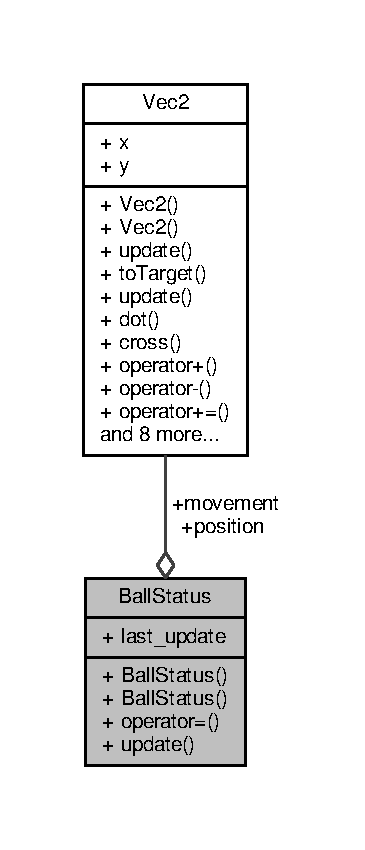
\includegraphics[width=175pt]{class_ball_status__coll__graph}
\end{center}
\end{figure}
\subsection*{Public Member Functions}
\begin{DoxyCompactItemize}
\item 
\hyperlink{class_ball_status_aa386a95ecc7b3968acd8f683587aa11c}{Ball\+Status} (float posx, float posy, float movementx, float movementy)
\item 
\hyperlink{class_ball_status_aa52a3da020cc2545b3c3fd8bd7944246}{Ball\+Status} ()
\item 
\hyperlink{class_ball_status}{Ball\+Status} \& \hyperlink{class_ball_status_a02508ed35c2fe08e41f99b3c1e36bffe}{operator=} (const \hyperlink{class_ball_status}{Ball\+Status} \&bs)
\item 
void \hyperlink{class_ball_status_a248375c08a18fd1d6975dd8e8bbf6923}{update} (float x, float y)
\end{DoxyCompactItemize}
\subsection*{Public Attributes}
\begin{DoxyCompactItemize}
\item 
\hyperlink{class_vec2}{Vec2} \hyperlink{class_ball_status_a8dce8cc463cb99e8bc8a02d8dd880e21}{movement}
\item 
\hyperlink{class_vec2}{Vec2} \hyperlink{class_ball_status_a7d841e95314cf93e4afbc894288a992b}{position}
\item 
clock\+\_\+t \hyperlink{class_ball_status_a8a53c0c35e7179f0af564142f9cccf1c}{last\+\_\+update}
\end{DoxyCompactItemize}


\subsection{Detailed Description}
\hyperlink{class_ball_status}{Ball\+Status} class 

\subsection{Constructor \& Destructor Documentation}
\index{Ball\+Status@{Ball\+Status}!Ball\+Status@{Ball\+Status}}
\index{Ball\+Status@{Ball\+Status}!Ball\+Status@{Ball\+Status}}
\subsubsection[{\texorpdfstring{Ball\+Status(float posx, float posy, float movementx, float movementy)}{BallStatus(float posx, float posy, float movementx, float movementy)}}]{\setlength{\rightskip}{0pt plus 5cm}Ball\+Status\+::\+Ball\+Status (
\begin{DoxyParamCaption}
\item[{float}]{posx, }
\item[{float}]{posy, }
\item[{float}]{movementx, }
\item[{float}]{movementy}
\end{DoxyParamCaption}
)\hspace{0.3cm}{\ttfamily [inline]}}\hypertarget{class_ball_status_aa386a95ecc7b3968acd8f683587aa11c}{}\label{class_ball_status_aa386a95ecc7b3968acd8f683587aa11c}
\hyperlink{class_ball_status}{Ball\+Status} constructor


\begin{DoxyParams}{Parameters}
{\em (float} & posx, float posy, float movementx, float movementy) \\
\hline
\end{DoxyParams}
\index{Ball\+Status@{Ball\+Status}!Ball\+Status@{Ball\+Status}}
\index{Ball\+Status@{Ball\+Status}!Ball\+Status@{Ball\+Status}}
\subsubsection[{\texorpdfstring{Ball\+Status()}{BallStatus()}}]{\setlength{\rightskip}{0pt plus 5cm}Ball\+Status\+::\+Ball\+Status (
\begin{DoxyParamCaption}
{}
\end{DoxyParamCaption}
)\hspace{0.3cm}{\ttfamily [inline]}}\hypertarget{class_ball_status_aa52a3da020cc2545b3c3fd8bd7944246}{}\label{class_ball_status_aa52a3da020cc2545b3c3fd8bd7944246}
\hyperlink{class_ball_status}{Ball\+Status} constructor 

\subsection{Member Function Documentation}
\index{Ball\+Status@{Ball\+Status}!operator=@{operator=}}
\index{operator=@{operator=}!Ball\+Status@{Ball\+Status}}
\subsubsection[{\texorpdfstring{operator=(const Ball\+Status \&bs)}{operator=(const BallStatus &bs)}}]{\setlength{\rightskip}{0pt plus 5cm}{\bf Ball\+Status}\& Ball\+Status\+::operator= (
\begin{DoxyParamCaption}
\item[{const {\bf Ball\+Status} \&}]{bs}
\end{DoxyParamCaption}
)\hspace{0.3cm}{\ttfamily [inline]}}\hypertarget{class_ball_status_a02508ed35c2fe08e41f99b3c1e36bffe}{}\label{class_ball_status_a02508ed35c2fe08e41f99b3c1e36bffe}
operator function


\begin{DoxyParams}{Parameters}
{\em (const} & \hyperlink{class_ball_status}{Ball\+Status} \& bs)\\
\hline
\end{DoxyParams}
\begin{DoxyReturn}{Returns}
$\ast$this 
\end{DoxyReturn}
\index{Ball\+Status@{Ball\+Status}!update@{update}}
\index{update@{update}!Ball\+Status@{Ball\+Status}}
\subsubsection[{\texorpdfstring{update(float x, float y)}{update(float x, float y)}}]{\setlength{\rightskip}{0pt plus 5cm}void Ball\+Status\+::update (
\begin{DoxyParamCaption}
\item[{float}]{x, }
\item[{float}]{y}
\end{DoxyParamCaption}
)\hspace{0.3cm}{\ttfamily [inline]}}\hypertarget{class_ball_status_a248375c08a18fd1d6975dd8e8bbf6923}{}\label{class_ball_status_a248375c08a18fd1d6975dd8e8bbf6923}
update function

Function to update the the ball status. It automatically calculates the resulting velocity.


\begin{DoxyParams}{Parameters}
{\em (float} & x, float y) \\
\hline
\end{DoxyParams}


Here is the call graph for this function\+:\nopagebreak
\begin{figure}[H]
\begin{center}
\leavevmode
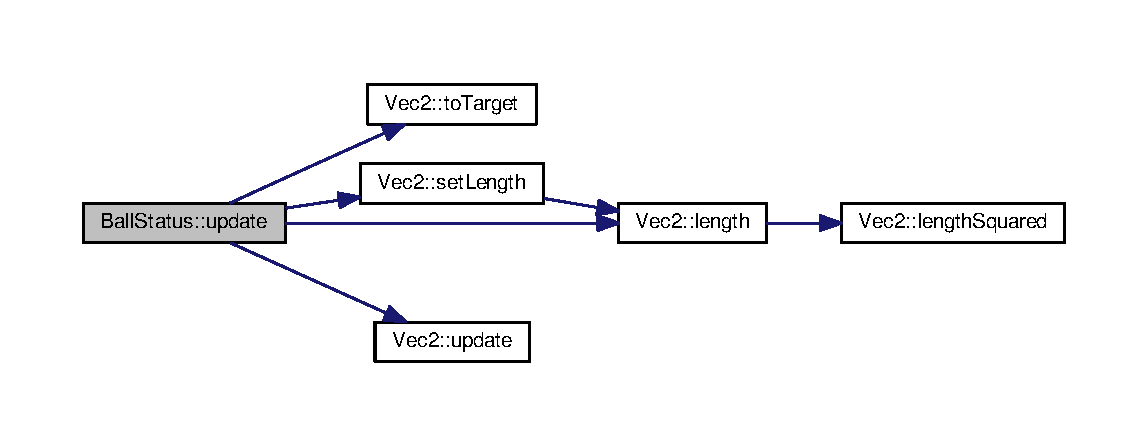
\includegraphics[width=350pt]{class_ball_status_a248375c08a18fd1d6975dd8e8bbf6923_cgraph}
\end{center}
\end{figure}




Here is the caller graph for this function\+:\nopagebreak
\begin{figure}[H]
\begin{center}
\leavevmode
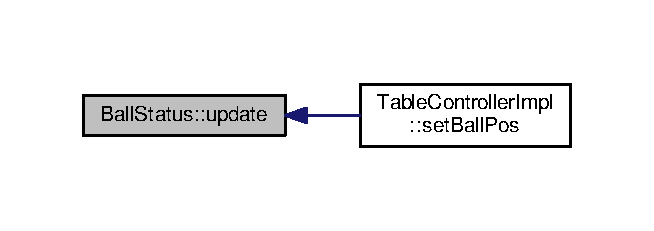
\includegraphics[width=314pt]{class_ball_status_a248375c08a18fd1d6975dd8e8bbf6923_icgraph}
\end{center}
\end{figure}




\subsection{Member Data Documentation}
\index{Ball\+Status@{Ball\+Status}!last\+\_\+update@{last\+\_\+update}}
\index{last\+\_\+update@{last\+\_\+update}!Ball\+Status@{Ball\+Status}}
\subsubsection[{\texorpdfstring{last\+\_\+update}{last_update}}]{\setlength{\rightskip}{0pt plus 5cm}clock\+\_\+t Ball\+Status\+::last\+\_\+update}\hypertarget{class_ball_status_a8a53c0c35e7179f0af564142f9cccf1c}{}\label{class_ball_status_a8a53c0c35e7179f0af564142f9cccf1c}
\index{Ball\+Status@{Ball\+Status}!movement@{movement}}
\index{movement@{movement}!Ball\+Status@{Ball\+Status}}
\subsubsection[{\texorpdfstring{movement}{movement}}]{\setlength{\rightskip}{0pt plus 5cm}{\bf Vec2} Ball\+Status\+::movement}\hypertarget{class_ball_status_a8dce8cc463cb99e8bc8a02d8dd880e21}{}\label{class_ball_status_a8dce8cc463cb99e8bc8a02d8dd880e21}
\index{Ball\+Status@{Ball\+Status}!position@{position}}
\index{position@{position}!Ball\+Status@{Ball\+Status}}
\subsubsection[{\texorpdfstring{position}{position}}]{\setlength{\rightskip}{0pt plus 5cm}{\bf Vec2} Ball\+Status\+::position}\hypertarget{class_ball_status_a7d841e95314cf93e4afbc894288a992b}{}\label{class_ball_status_a7d841e95314cf93e4afbc894288a992b}


The documentation for this class was generated from the following file\+:\begin{DoxyCompactItemize}
\item 
Kick\+I\+T@\+Eclipse/5\+\_\+\+Data\+Type/\hyperlink{_ball_status_8hpp}{Ball\+Status.\+hpp}\end{DoxyCompactItemize}

\hypertarget{class_ball_tracker_impl}{}\section{Ball\+Tracker\+Impl Class Reference}
\label{class_ball_tracker_impl}\index{Ball\+Tracker\+Impl@{Ball\+Tracker\+Impl}}


{\ttfamily \#include $<$Ball\+Tracker\+Impl.\+hpp$>$}



Inheritance diagram for Ball\+Tracker\+Impl\+:\nopagebreak
\begin{figure}[H]
\begin{center}
\leavevmode
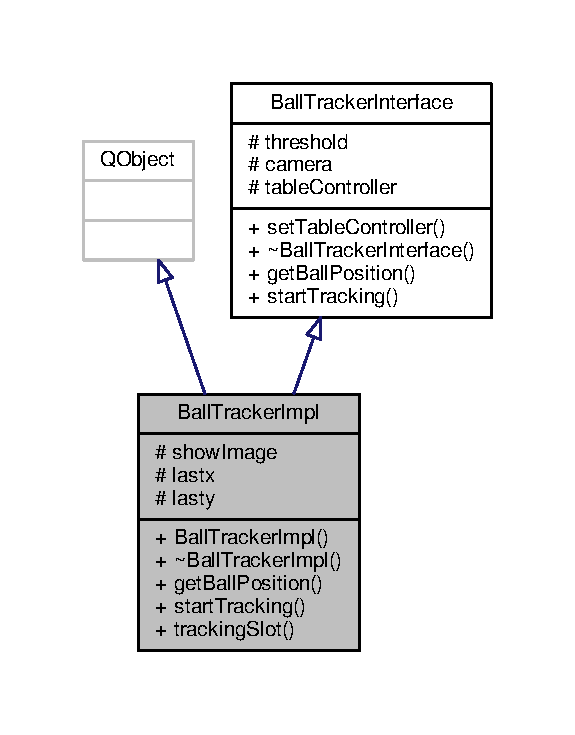
\includegraphics[width=276pt]{class_ball_tracker_impl__inherit__graph}
\end{center}
\end{figure}


Collaboration diagram for Ball\+Tracker\+Impl\+:\nopagebreak
\begin{figure}[H]
\begin{center}
\leavevmode
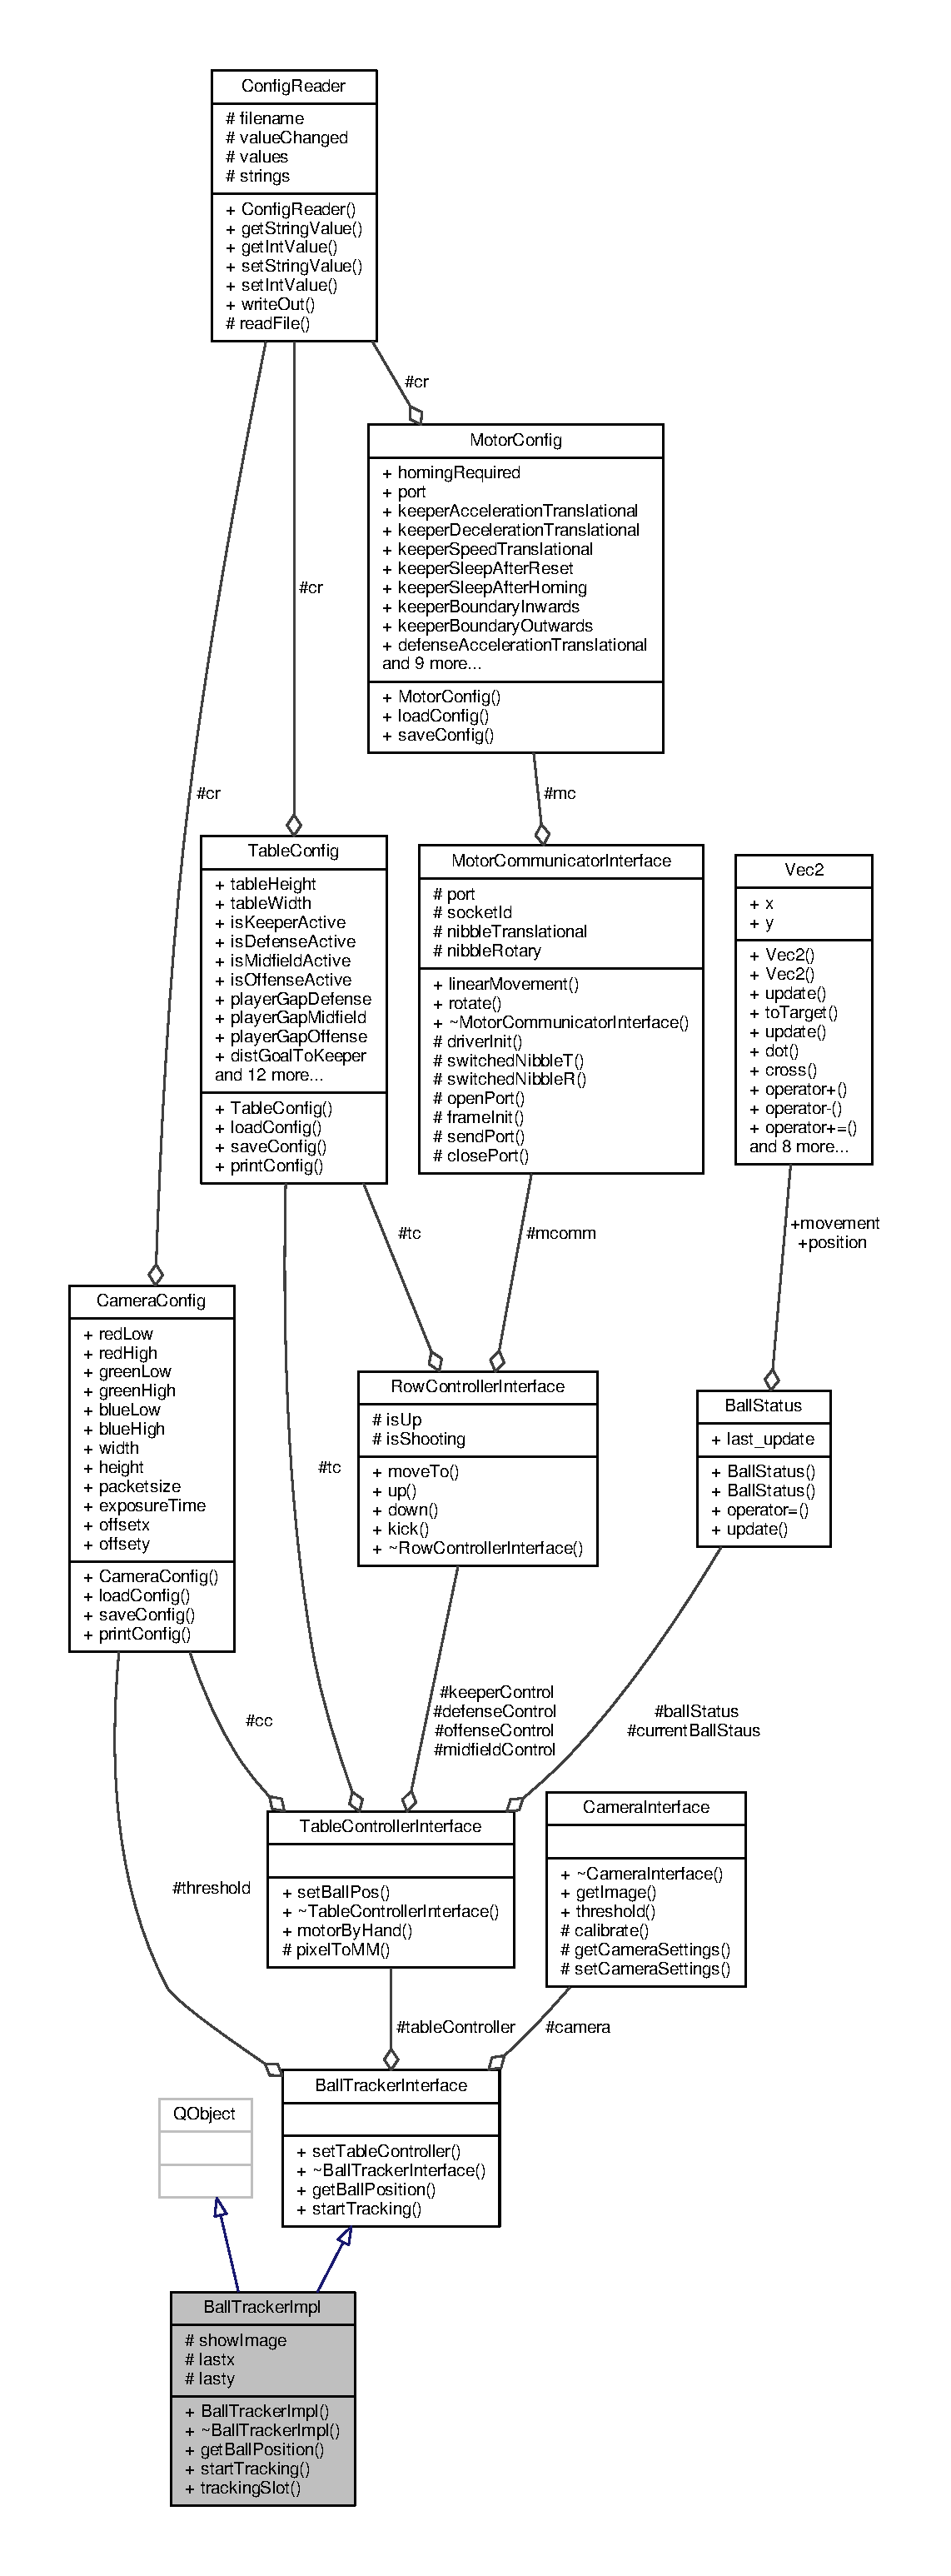
\includegraphics[height=550pt]{class_ball_tracker_impl__coll__graph}
\end{center}
\end{figure}
\subsection*{Public Slots}
\begin{DoxyCompactItemize}
\item 
void \hyperlink{class_ball_tracker_impl_a4a66db042c2b4a2f0c2f76c6c9fbfa96}{tracking\+Slot} ()
\end{DoxyCompactItemize}
\subsection*{Public Member Functions}
\begin{DoxyCompactItemize}
\item 
\hyperlink{class_ball_tracker_impl_a286916fd3631fd8dfffaa099f5ac1ace}{Ball\+Tracker\+Impl} (\hyperlink{class_table_controller_interface}{Table\+Controller\+Interface} $\ast$tci)
\item 
\hyperlink{class_ball_tracker_impl_ac0c591a55c71d4a4f62e44c32ef64432}{$\sim$\+Ball\+Tracker\+Impl} ()
\item 
\hyperlink{class_vec2}{Vec2} \hyperlink{class_ball_tracker_impl_a6edec8b002aa9e81b422cce0165e3b32}{get\+Ball\+Position} ()
\item 
void \hyperlink{class_ball_tracker_impl_adafeb5b7297cc09a42fdcd00aa52b367}{start\+Tracking} ()
\end{DoxyCompactItemize}
\subsection*{Protected Attributes}
\begin{DoxyCompactItemize}
\item 
bool \hyperlink{class_ball_tracker_impl_ad8ac7539ec3de2bb0657048366677bfa}{show\+Image} = true
\item 
double \hyperlink{class_ball_tracker_impl_a9588e1cae36137cab8f815802f9bbf22}{lastx} = 0
\item 
double \hyperlink{class_ball_tracker_impl_a350b9d1e03a2191baed4f33c11c7217e}{lasty} = 0
\end{DoxyCompactItemize}


\subsection{Detailed Description}
\hyperlink{class_ball_tracker_impl}{Ball\+Tracker\+Impl} class

öaldighjseldkgnlrcktuj sdtjhdtzjrzbukbtiul guzlozu9löziol 

\subsection{Constructor \& Destructor Documentation}
\index{Ball\+Tracker\+Impl@{Ball\+Tracker\+Impl}!Ball\+Tracker\+Impl@{Ball\+Tracker\+Impl}}
\index{Ball\+Tracker\+Impl@{Ball\+Tracker\+Impl}!Ball\+Tracker\+Impl@{Ball\+Tracker\+Impl}}
\subsubsection[{\texorpdfstring{Ball\+Tracker\+Impl(\+Table\+Controller\+Interface $\ast$tci)}{BallTrackerImpl(TableControllerInterface *tci)}}]{\setlength{\rightskip}{0pt plus 5cm}Ball\+Tracker\+Impl\+::\+Ball\+Tracker\+Impl (
\begin{DoxyParamCaption}
\item[{{\bf Table\+Controller\+Interface} $\ast$}]{tci}
\end{DoxyParamCaption}
)}\hypertarget{class_ball_tracker_impl_a286916fd3631fd8dfffaa099f5ac1ace}{}\label{class_ball_tracker_impl_a286916fd3631fd8dfffaa099f5ac1ace}
\hyperlink{class_ball_tracker_impl}{Ball\+Tracker\+Impl} constructor 
\begin{DoxyParams}{Parameters}
{\em Table\+Controller\+Interface$\ast$} & tci\\
\hline
\end{DoxyParams}
If the Ball\+Tracker has detected a new ball position, the Table\+Controller must be notified \index{Ball\+Tracker\+Impl@{Ball\+Tracker\+Impl}!````~Ball\+Tracker\+Impl@{$\sim$\+Ball\+Tracker\+Impl}}
\index{````~Ball\+Tracker\+Impl@{$\sim$\+Ball\+Tracker\+Impl}!Ball\+Tracker\+Impl@{Ball\+Tracker\+Impl}}
\subsubsection[{\texorpdfstring{$\sim$\+Ball\+Tracker\+Impl()}{~BallTrackerImpl()}}]{\setlength{\rightskip}{0pt plus 5cm}Ball\+Tracker\+Impl\+::$\sim$\+Ball\+Tracker\+Impl (
\begin{DoxyParamCaption}
{}
\end{DoxyParamCaption}
)}\hypertarget{class_ball_tracker_impl_ac0c591a55c71d4a4f62e44c32ef64432}{}\label{class_ball_tracker_impl_ac0c591a55c71d4a4f62e44c32ef64432}
\hyperlink{class_ball_tracker_impl}{Ball\+Tracker\+Impl} destructor 

\subsection{Member Function Documentation}
\index{Ball\+Tracker\+Impl@{Ball\+Tracker\+Impl}!get\+Ball\+Position@{get\+Ball\+Position}}
\index{get\+Ball\+Position@{get\+Ball\+Position}!Ball\+Tracker\+Impl@{Ball\+Tracker\+Impl}}
\subsubsection[{\texorpdfstring{get\+Ball\+Position()}{getBallPosition()}}]{\setlength{\rightskip}{0pt plus 5cm}{\bf Vec2} Ball\+Tracker\+Impl\+::get\+Ball\+Position (
\begin{DoxyParamCaption}
{}
\end{DoxyParamCaption}
)\hspace{0.3cm}{\ttfamily [virtual]}}\hypertarget{class_ball_tracker_impl_a6edec8b002aa9e81b422cce0165e3b32}{}\label{class_ball_tracker_impl_a6edec8b002aa9e81b422cce0165e3b32}
get\+Ball\+Position function

testtestsetaelöighaoit8zkthl 

Implements \hyperlink{class_ball_tracker_interface_a4a15d76099b49ef842a87dbabbac1b07}{Ball\+Tracker\+Interface}.

\index{Ball\+Tracker\+Impl@{Ball\+Tracker\+Impl}!start\+Tracking@{start\+Tracking}}
\index{start\+Tracking@{start\+Tracking}!Ball\+Tracker\+Impl@{Ball\+Tracker\+Impl}}
\subsubsection[{\texorpdfstring{start\+Tracking()}{startTracking()}}]{\setlength{\rightskip}{0pt plus 5cm}void Ball\+Tracker\+Impl\+::start\+Tracking (
\begin{DoxyParamCaption}
{}
\end{DoxyParamCaption}
)\hspace{0.3cm}{\ttfamily [virtual]}}\hypertarget{class_ball_tracker_impl_adafeb5b7297cc09a42fdcd00aa52b367}{}\label{class_ball_tracker_impl_adafeb5b7297cc09a42fdcd00aa52b367}
start\+Tracking function 

Implements \hyperlink{class_ball_tracker_interface_af140a5a17f082a74ff06bee64ef055ba}{Ball\+Tracker\+Interface}.



Here is the caller graph for this function\+:\nopagebreak
\begin{figure}[H]
\begin{center}
\leavevmode
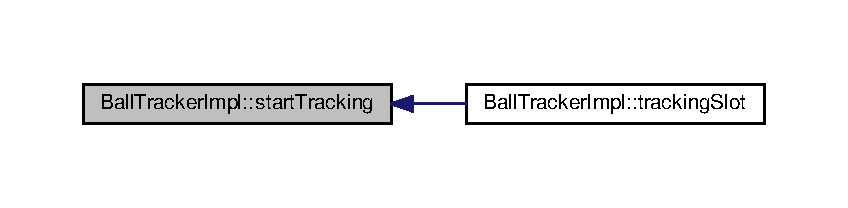
\includegraphics[width=350pt]{class_ball_tracker_impl_adafeb5b7297cc09a42fdcd00aa52b367_icgraph}
\end{center}
\end{figure}


\index{Ball\+Tracker\+Impl@{Ball\+Tracker\+Impl}!tracking\+Slot@{tracking\+Slot}}
\index{tracking\+Slot@{tracking\+Slot}!Ball\+Tracker\+Impl@{Ball\+Tracker\+Impl}}
\subsubsection[{\texorpdfstring{tracking\+Slot}{trackingSlot}}]{\setlength{\rightskip}{0pt plus 5cm}void Ball\+Tracker\+Impl\+::tracking\+Slot (
\begin{DoxyParamCaption}
{}
\end{DoxyParamCaption}
)\hspace{0.3cm}{\ttfamily [inline]}, {\ttfamily [slot]}}\hypertarget{class_ball_tracker_impl_a4a66db042c2b4a2f0c2f76c6c9fbfa96}{}\label{class_ball_tracker_impl_a4a66db042c2b4a2f0c2f76c6c9fbfa96}
tracking\+Slot function 

Here is the call graph for this function\+:\nopagebreak
\begin{figure}[H]
\begin{center}
\leavevmode
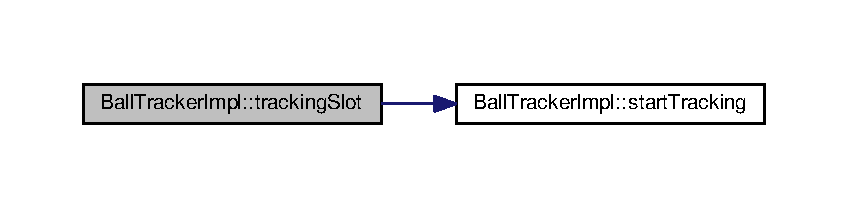
\includegraphics[width=350pt]{class_ball_tracker_impl_a4a66db042c2b4a2f0c2f76c6c9fbfa96_cgraph}
\end{center}
\end{figure}




\subsection{Member Data Documentation}
\index{Ball\+Tracker\+Impl@{Ball\+Tracker\+Impl}!lastx@{lastx}}
\index{lastx@{lastx}!Ball\+Tracker\+Impl@{Ball\+Tracker\+Impl}}
\subsubsection[{\texorpdfstring{lastx}{lastx}}]{\setlength{\rightskip}{0pt plus 5cm}double Ball\+Tracker\+Impl\+::lastx = 0\hspace{0.3cm}{\ttfamily [protected]}}\hypertarget{class_ball_tracker_impl_a9588e1cae36137cab8f815802f9bbf22}{}\label{class_ball_tracker_impl_a9588e1cae36137cab8f815802f9bbf22}
\index{Ball\+Tracker\+Impl@{Ball\+Tracker\+Impl}!lasty@{lasty}}
\index{lasty@{lasty}!Ball\+Tracker\+Impl@{Ball\+Tracker\+Impl}}
\subsubsection[{\texorpdfstring{lasty}{lasty}}]{\setlength{\rightskip}{0pt plus 5cm}double Ball\+Tracker\+Impl\+::lasty = 0\hspace{0.3cm}{\ttfamily [protected]}}\hypertarget{class_ball_tracker_impl_a350b9d1e03a2191baed4f33c11c7217e}{}\label{class_ball_tracker_impl_a350b9d1e03a2191baed4f33c11c7217e}
\index{Ball\+Tracker\+Impl@{Ball\+Tracker\+Impl}!show\+Image@{show\+Image}}
\index{show\+Image@{show\+Image}!Ball\+Tracker\+Impl@{Ball\+Tracker\+Impl}}
\subsubsection[{\texorpdfstring{show\+Image}{showImage}}]{\setlength{\rightskip}{0pt plus 5cm}bool Ball\+Tracker\+Impl\+::show\+Image = true\hspace{0.3cm}{\ttfamily [protected]}}\hypertarget{class_ball_tracker_impl_ad8ac7539ec3de2bb0657048366677bfa}{}\label{class_ball_tracker_impl_ad8ac7539ec3de2bb0657048366677bfa}


The documentation for this class was generated from the following files\+:\begin{DoxyCompactItemize}
\item 
1\+\_\+\+Ball\+Tracking/\+Ball\+Tracker/\hyperlink{_ball_tracker_impl_8hpp}{Ball\+Tracker\+Impl.\+hpp}\item 
1\+\_\+\+Ball\+Tracking/\+Ball\+Tracker/\hyperlink{_ball_tracker_impl_8cpp}{Ball\+Tracker\+Impl.\+cpp}\end{DoxyCompactItemize}

\hypertarget{class_ball_tracker_interface}{}\section{Ball\+Tracker\+Interface Class Reference}
\label{class_ball_tracker_interface}\index{Ball\+Tracker\+Interface@{Ball\+Tracker\+Interface}}


{\ttfamily \#include $<$\+\_\+\+Ball\+Tracker\+Interface.\+hpp$>$}



Inheritance diagram for Ball\+Tracker\+Interface\+:\nopagebreak
\begin{figure}[H]
\begin{center}
\leavevmode
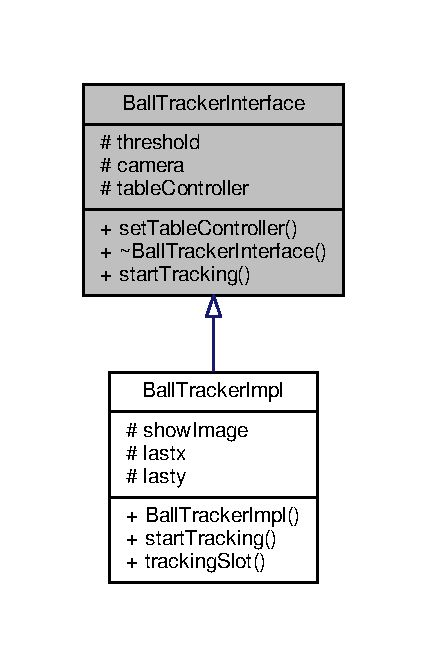
\includegraphics[width=205pt]{class_ball_tracker_interface__inherit__graph}
\end{center}
\end{figure}


Collaboration diagram for Ball\+Tracker\+Interface\+:\nopagebreak
\begin{figure}[H]
\begin{center}
\leavevmode
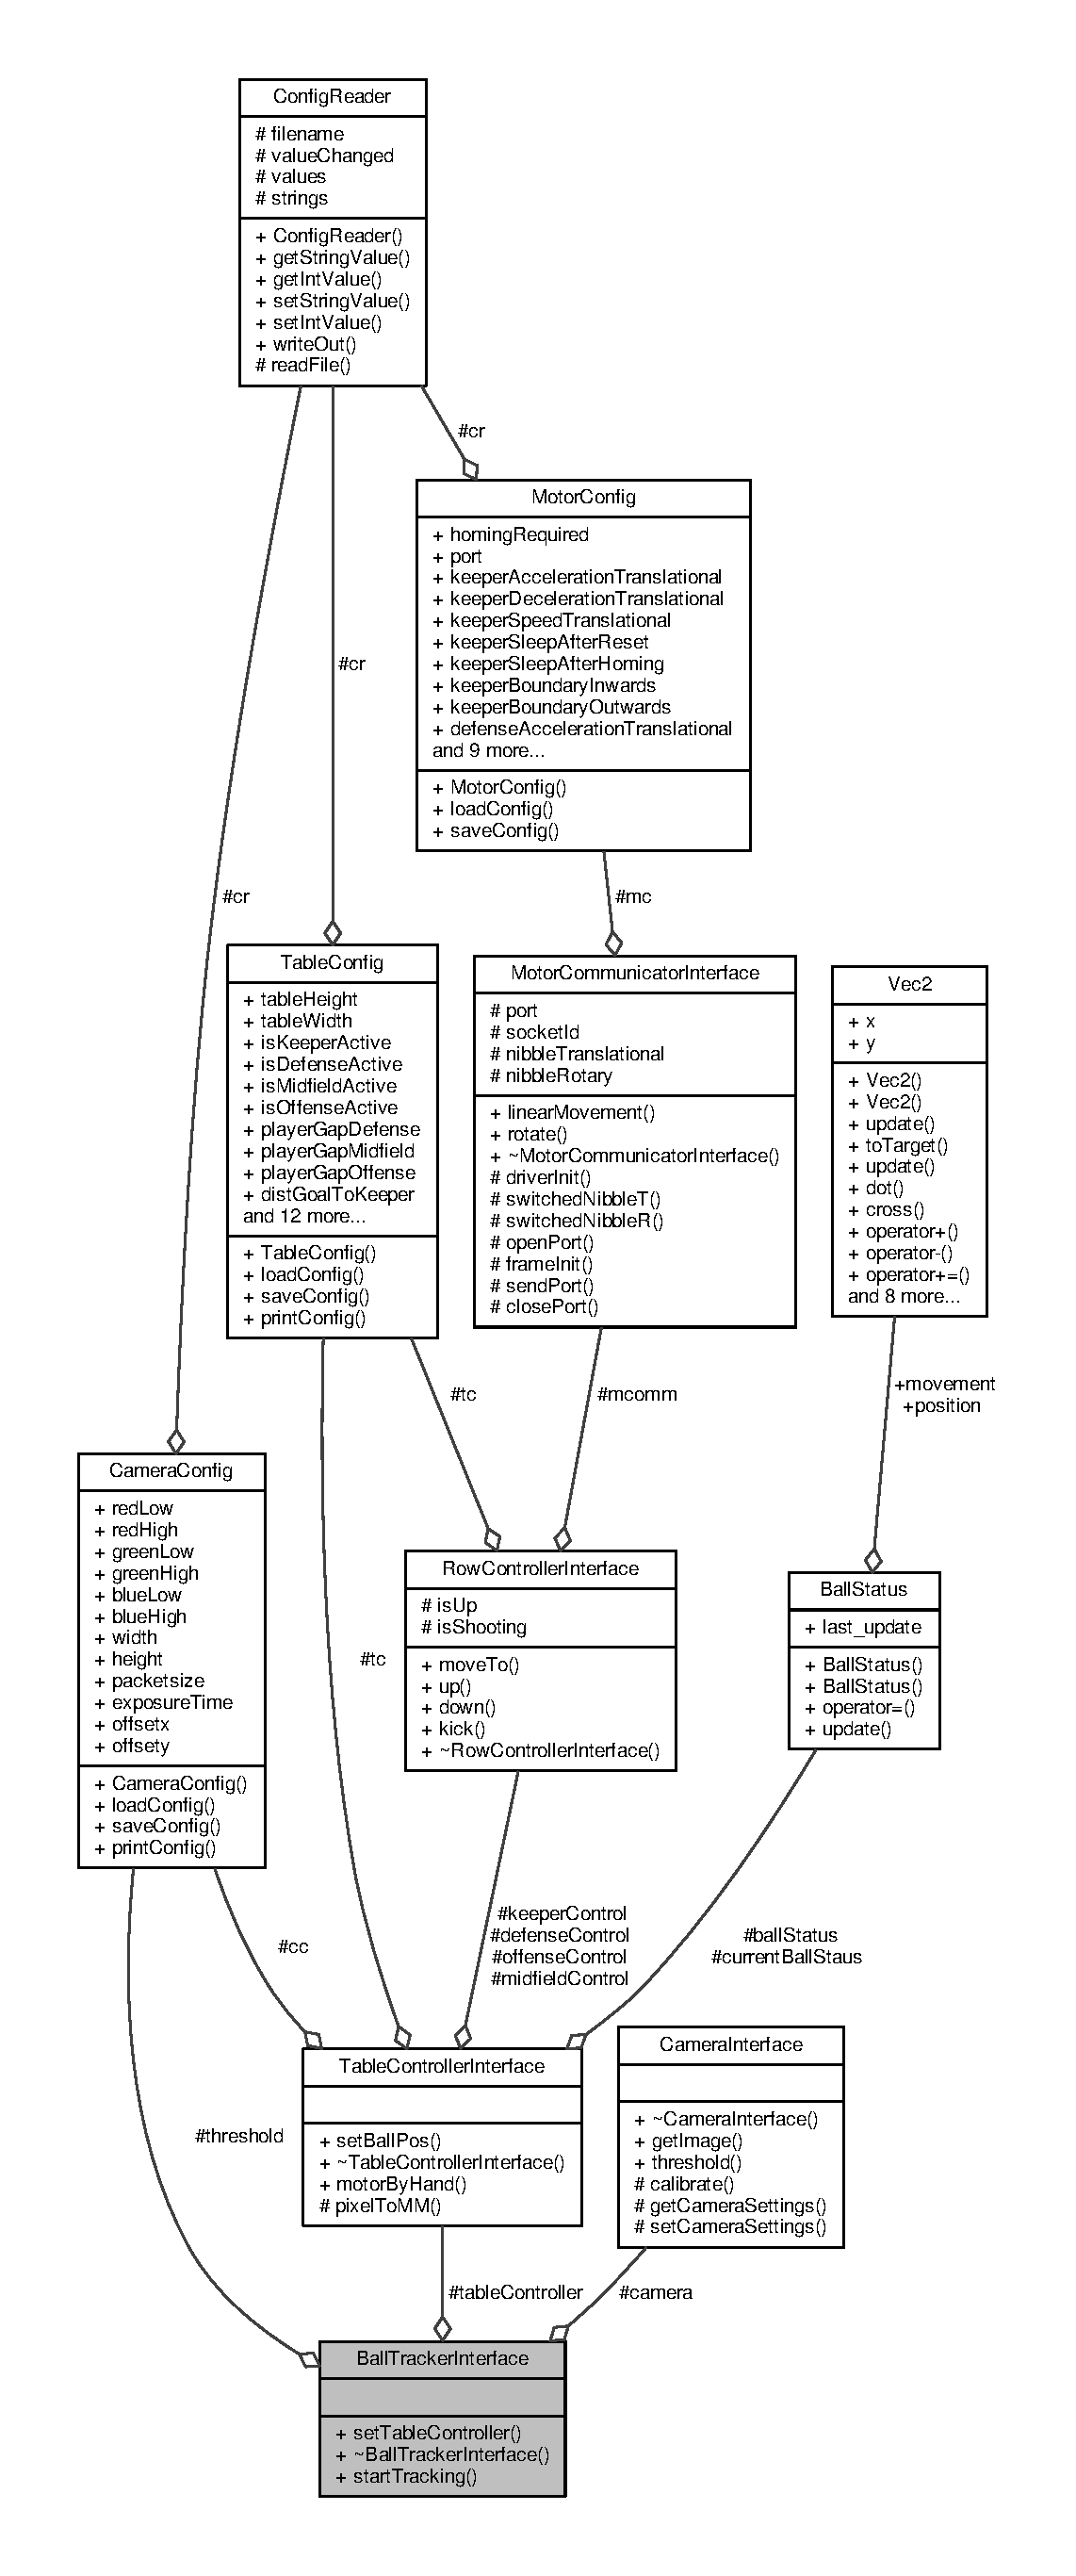
\includegraphics[height=550pt]{class_ball_tracker_interface__coll__graph}
\end{center}
\end{figure}
\subsection*{Public Member Functions}
\begin{DoxyCompactItemize}
\item 
void \hyperlink{class_ball_tracker_interface_a009a2a29aa7993a2405741daf707afbb}{set\+Table\+Controller} (\hyperlink{class_table_controller_interface}{Table\+Controller\+Interface} $\ast$t)
\item 
virtual \hyperlink{class_ball_tracker_interface_a85a4559b18c41e1a88da092ab8a7f42d}{$\sim$\+Ball\+Tracker\+Interface} ()
\item 
virtual void \hyperlink{class_ball_tracker_interface_af140a5a17f082a74ff06bee64ef055ba}{start\+Tracking} ()=0
\end{DoxyCompactItemize}
\subsection*{Protected Attributes}
\begin{DoxyCompactItemize}
\item 
\hyperlink{class_camera_config}{Camera\+Config} $\ast$ \hyperlink{class_ball_tracker_interface_ae6c6c4c3d89a8cc65bceec6c56af3b62}{threshold}
\item 
\hyperlink{class_camera_interface}{Camera\+Interface} $\ast$ \hyperlink{class_ball_tracker_interface_a48d727df5926f57a6cd5c2b75d039604}{camera}
\item 
\hyperlink{class_table_controller_interface}{Table\+Controller\+Interface} $\ast$ \hyperlink{class_ball_tracker_interface_a1716b6f0ad84d9d68da4dec0955450bf}{table\+Controller}
\end{DoxyCompactItemize}


\subsection{Detailed Description}
\hyperlink{class_ball_tracker_interface}{Ball\+Tracker\+Interface} class 

\subsection{Constructor \& Destructor Documentation}
\index{Ball\+Tracker\+Interface@{Ball\+Tracker\+Interface}!````~Ball\+Tracker\+Interface@{$\sim$\+Ball\+Tracker\+Interface}}
\index{````~Ball\+Tracker\+Interface@{$\sim$\+Ball\+Tracker\+Interface}!Ball\+Tracker\+Interface@{Ball\+Tracker\+Interface}}
\subsubsection[{\texorpdfstring{$\sim$\+Ball\+Tracker\+Interface()}{~BallTrackerInterface()}}]{\setlength{\rightskip}{0pt plus 5cm}virtual Ball\+Tracker\+Interface\+::$\sim$\+Ball\+Tracker\+Interface (
\begin{DoxyParamCaption}
{}
\end{DoxyParamCaption}
)\hspace{0.3cm}{\ttfamily [inline]}, {\ttfamily [virtual]}}\hypertarget{class_ball_tracker_interface_a85a4559b18c41e1a88da092ab8a7f42d}{}\label{class_ball_tracker_interface_a85a4559b18c41e1a88da092ab8a7f42d}
\hyperlink{class_ball_tracker_interface}{Ball\+Tracker\+Interface} destructor 

Here is the call graph for this function\+:\nopagebreak
\begin{figure}[H]
\begin{center}
\leavevmode
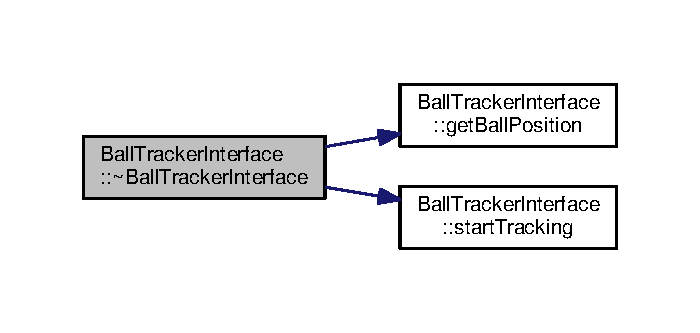
\includegraphics[width=336pt]{class_ball_tracker_interface_a85a4559b18c41e1a88da092ab8a7f42d_cgraph}
\end{center}
\end{figure}




\subsection{Member Function Documentation}
\index{Ball\+Tracker\+Interface@{Ball\+Tracker\+Interface}!set\+Table\+Controller@{set\+Table\+Controller}}
\index{set\+Table\+Controller@{set\+Table\+Controller}!Ball\+Tracker\+Interface@{Ball\+Tracker\+Interface}}
\subsubsection[{\texorpdfstring{set\+Table\+Controller(\+Table\+Controller\+Interface $\ast$t)}{setTableController(TableControllerInterface *t)}}]{\setlength{\rightskip}{0pt plus 5cm}void Ball\+Tracker\+Interface\+::set\+Table\+Controller (
\begin{DoxyParamCaption}
\item[{{\bf Table\+Controller\+Interface} $\ast$}]{t}
\end{DoxyParamCaption}
)\hspace{0.3cm}{\ttfamily [inline]}}\hypertarget{class_ball_tracker_interface_a009a2a29aa7993a2405741daf707afbb}{}\label{class_ball_tracker_interface_a009a2a29aa7993a2405741daf707afbb}
set\+Table\+Controller function


\begin{DoxyParams}{Parameters}
{\em (\+Table\+Controller\+Interface$\ast$} & t) \\
\hline
\end{DoxyParams}
\index{Ball\+Tracker\+Interface@{Ball\+Tracker\+Interface}!start\+Tracking@{start\+Tracking}}
\index{start\+Tracking@{start\+Tracking}!Ball\+Tracker\+Interface@{Ball\+Tracker\+Interface}}
\subsubsection[{\texorpdfstring{start\+Tracking()=0}{startTracking()=0}}]{\setlength{\rightskip}{0pt plus 5cm}virtual void Ball\+Tracker\+Interface\+::start\+Tracking (
\begin{DoxyParamCaption}
{}
\end{DoxyParamCaption}
)\hspace{0.3cm}{\ttfamily [pure virtual]}}\hypertarget{class_ball_tracker_interface_af140a5a17f082a74ff06bee64ef055ba}{}\label{class_ball_tracker_interface_af140a5a17f082a74ff06bee64ef055ba}
start\+Tracking function

Balltracking-\/loop. Continuously detects the position of the ball. 

Implemented in \hyperlink{class_ball_tracker_impl_adafeb5b7297cc09a42fdcd00aa52b367}{Ball\+Tracker\+Impl}.



Here is the caller graph for this function\+:\nopagebreak
\begin{figure}[H]
\begin{center}
\leavevmode
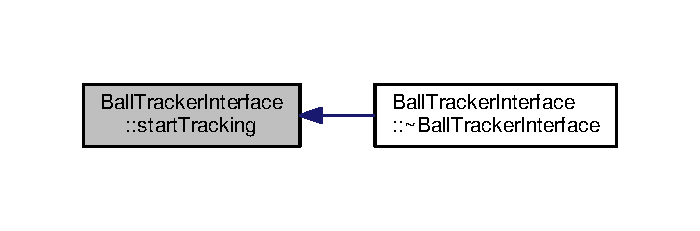
\includegraphics[width=336pt]{class_ball_tracker_interface_af140a5a17f082a74ff06bee64ef055ba_icgraph}
\end{center}
\end{figure}




\subsection{Member Data Documentation}
\index{Ball\+Tracker\+Interface@{Ball\+Tracker\+Interface}!camera@{camera}}
\index{camera@{camera}!Ball\+Tracker\+Interface@{Ball\+Tracker\+Interface}}
\subsubsection[{\texorpdfstring{camera}{camera}}]{\setlength{\rightskip}{0pt plus 5cm}{\bf Camera\+Interface}$\ast$ Ball\+Tracker\+Interface\+::camera\hspace{0.3cm}{\ttfamily [protected]}}\hypertarget{class_ball_tracker_interface_a48d727df5926f57a6cd5c2b75d039604}{}\label{class_ball_tracker_interface_a48d727df5926f57a6cd5c2b75d039604}
\index{Ball\+Tracker\+Interface@{Ball\+Tracker\+Interface}!table\+Controller@{table\+Controller}}
\index{table\+Controller@{table\+Controller}!Ball\+Tracker\+Interface@{Ball\+Tracker\+Interface}}
\subsubsection[{\texorpdfstring{table\+Controller}{tableController}}]{\setlength{\rightskip}{0pt plus 5cm}{\bf Table\+Controller\+Interface}$\ast$ Ball\+Tracker\+Interface\+::table\+Controller\hspace{0.3cm}{\ttfamily [protected]}}\hypertarget{class_ball_tracker_interface_a1716b6f0ad84d9d68da4dec0955450bf}{}\label{class_ball_tracker_interface_a1716b6f0ad84d9d68da4dec0955450bf}
\index{Ball\+Tracker\+Interface@{Ball\+Tracker\+Interface}!threshold@{threshold}}
\index{threshold@{threshold}!Ball\+Tracker\+Interface@{Ball\+Tracker\+Interface}}
\subsubsection[{\texorpdfstring{threshold}{threshold}}]{\setlength{\rightskip}{0pt plus 5cm}{\bf Camera\+Config}$\ast$ Ball\+Tracker\+Interface\+::threshold\hspace{0.3cm}{\ttfamily [protected]}}\hypertarget{class_ball_tracker_interface_ae6c6c4c3d89a8cc65bceec6c56af3b62}{}\label{class_ball_tracker_interface_ae6c6c4c3d89a8cc65bceec6c56af3b62}


The documentation for this class was generated from the following file\+:\begin{DoxyCompactItemize}
\item 
Kick\+I\+T@\+Eclipse/1\+\_\+\+Ball\+Tracking/\+Ball\+Tracker/\hyperlink{___ball_tracker_interface_8hpp}{\+\_\+\+Ball\+Tracker\+Interface.\+hpp}\end{DoxyCompactItemize}

\hypertarget{class_camera}{}\section{Camera Class Reference}
\label{class_camera}\index{Camera@{Camera}}


{\ttfamily \#include $<$Camera.\+hpp$>$}



Inheritance diagram for Camera\+:\nopagebreak
\begin{figure}[H]
\begin{center}
\leavevmode
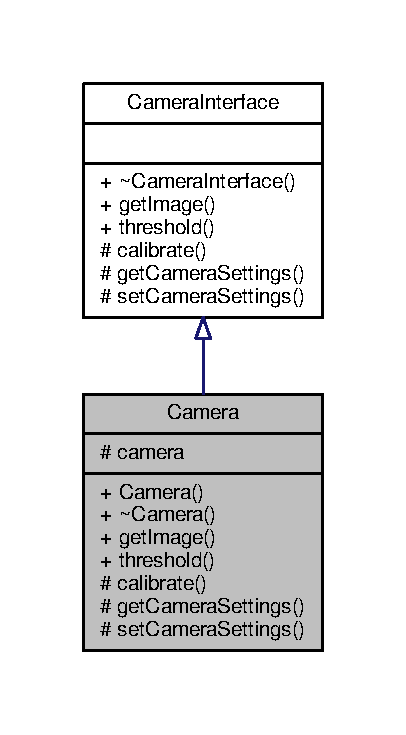
\includegraphics[width=195pt]{class_camera__inherit__graph}
\end{center}
\end{figure}


Collaboration diagram for Camera\+:\nopagebreak
\begin{figure}[H]
\begin{center}
\leavevmode
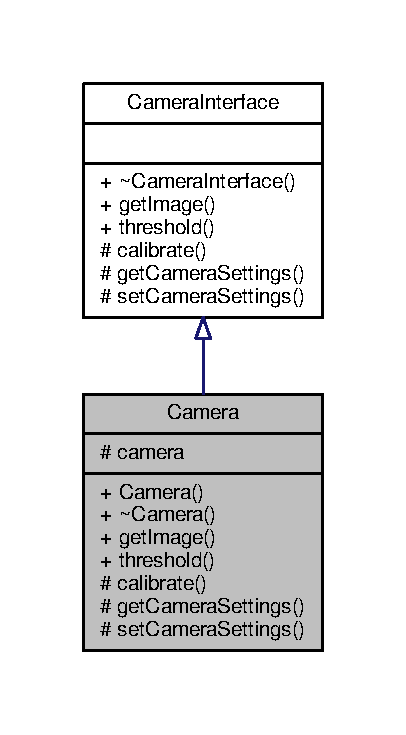
\includegraphics[width=195pt]{class_camera__coll__graph}
\end{center}
\end{figure}
\subsection*{Public Member Functions}
\begin{DoxyCompactItemize}
\item 
\hyperlink{class_camera_a01f94c3543f56ede7af49dc778f19331}{Camera} ()
\item 
virtual \hyperlink{class_camera_ad1897942d0ccf91052386388a497349f}{$\sim$\+Camera} ()
\item 
cv\+::\+Mat $\ast$ \hyperlink{class_camera_a45c96b9b33d73f3a5af527de0a5b6526}{get\+Image} ()
\item 
\hyperlink{class_camera_config}{Camera\+Config} $\ast$ \hyperlink{class_camera_ad4553e7cd83dba29a3d0b1542e28c66e}{threshold} ()
\end{DoxyCompactItemize}
\subsection*{Protected Member Functions}
\begin{DoxyCompactItemize}
\item 
void \hyperlink{class_camera_aff4f0478ef6ed7b35f353a6d055f0481}{calibrate} ()
\item 
void \hyperlink{class_camera_a62e9e0757dc2758b118274cfa5d56ff6}{get\+Camera\+Settings} ()
\item 
void \hyperlink{class_camera_afc0e7093a6749fa1445545cd59fca7b0}{set\+Camera\+Settings} ()
\end{DoxyCompactItemize}
\subsection*{Protected Attributes}
\begin{DoxyCompactItemize}
\item 
C\+Instant\+Camera $\ast$ \hyperlink{class_camera_ade18caead38b42ad3ea4ca3816452996}{camera}
\end{DoxyCompactItemize}


\subsection{Detailed Description}
Cammera\+Interface class 

\subsection{Constructor \& Destructor Documentation}
\index{Camera@{Camera}!Camera@{Camera}}
\index{Camera@{Camera}!Camera@{Camera}}
\subsubsection[{\texorpdfstring{Camera()}{Camera()}}]{\setlength{\rightskip}{0pt plus 5cm}Camera\+::\+Camera (
\begin{DoxyParamCaption}
{}
\end{DoxyParamCaption}
)}\hypertarget{class_camera_a01f94c3543f56ede7af49dc778f19331}{}\label{class_camera_a01f94c3543f56ede7af49dc778f19331}
\hyperlink{class_camera}{Camera} constructor \index{Camera@{Camera}!````~Camera@{$\sim$\+Camera}}
\index{````~Camera@{$\sim$\+Camera}!Camera@{Camera}}
\subsubsection[{\texorpdfstring{$\sim$\+Camera()}{~Camera()}}]{\setlength{\rightskip}{0pt plus 5cm}Camera\+::$\sim$\+Camera (
\begin{DoxyParamCaption}
{}
\end{DoxyParamCaption}
)\hspace{0.3cm}{\ttfamily [virtual]}}\hypertarget{class_camera_ad1897942d0ccf91052386388a497349f}{}\label{class_camera_ad1897942d0ccf91052386388a497349f}
\hyperlink{class_camera}{Camera} destructor 

\subsection{Member Function Documentation}
\index{Camera@{Camera}!calibrate@{calibrate}}
\index{calibrate@{calibrate}!Camera@{Camera}}
\subsubsection[{\texorpdfstring{calibrate()}{calibrate()}}]{\setlength{\rightskip}{0pt plus 5cm}void Camera\+::calibrate (
\begin{DoxyParamCaption}
{}
\end{DoxyParamCaption}
)\hspace{0.3cm}{\ttfamily [protected]}, {\ttfamily [virtual]}}\hypertarget{class_camera_aff4f0478ef6ed7b35f353a6d055f0481}{}\label{class_camera_aff4f0478ef6ed7b35f353a6d055f0481}
calibrate function wird nicht verwendet 

Implements \hyperlink{class_camera_interface_aba26bdb1e274ed311e2a5492df576f43}{Camera\+Interface}.

\index{Camera@{Camera}!get\+Camera\+Settings@{get\+Camera\+Settings}}
\index{get\+Camera\+Settings@{get\+Camera\+Settings}!Camera@{Camera}}
\subsubsection[{\texorpdfstring{get\+Camera\+Settings()}{getCameraSettings()}}]{\setlength{\rightskip}{0pt plus 5cm}void Camera\+::get\+Camera\+Settings (
\begin{DoxyParamCaption}
{}
\end{DoxyParamCaption}
)\hspace{0.3cm}{\ttfamily [protected]}, {\ttfamily [virtual]}}\hypertarget{class_camera_a62e9e0757dc2758b118274cfa5d56ff6}{}\label{class_camera_a62e9e0757dc2758b118274cfa5d56ff6}
get\+Camera\+Settings function gives the adjusted values of the camera 

Implements \hyperlink{class_camera_interface_af2abfcc95ea81477abbd0e9c4658b710}{Camera\+Interface}.

\index{Camera@{Camera}!get\+Image@{get\+Image}}
\index{get\+Image@{get\+Image}!Camera@{Camera}}
\subsubsection[{\texorpdfstring{get\+Image()}{getImage()}}]{\setlength{\rightskip}{0pt plus 5cm}cv\+::\+Mat $\ast$ Camera\+::get\+Image (
\begin{DoxyParamCaption}
{}
\end{DoxyParamCaption}
)\hspace{0.3cm}{\ttfamily [virtual]}}\hypertarget{class_camera_a45c96b9b33d73f3a5af527de0a5b6526}{}\label{class_camera_a45c96b9b33d73f3a5af527de0a5b6526}
get\+Image function Function retrieves a picture from the camera \begin{DoxyReturn}{Returns}
An image is returned 
\end{DoxyReturn}


Implements \hyperlink{class_camera_interface_a6e2e28f113f9db832f0e26c6c9c2a65e}{Camera\+Interface}.

\index{Camera@{Camera}!set\+Camera\+Settings@{set\+Camera\+Settings}}
\index{set\+Camera\+Settings@{set\+Camera\+Settings}!Camera@{Camera}}
\subsubsection[{\texorpdfstring{set\+Camera\+Settings()}{setCameraSettings()}}]{\setlength{\rightskip}{0pt plus 5cm}void Camera\+::set\+Camera\+Settings (
\begin{DoxyParamCaption}
{}
\end{DoxyParamCaption}
)\hspace{0.3cm}{\ttfamily [protected]}, {\ttfamily [virtual]}}\hypertarget{class_camera_afc0e7093a6749fa1445545cd59fca7b0}{}\label{class_camera_afc0e7093a6749fa1445545cd59fca7b0}
set\+Camera\+Settings Function for initial configuration of the camera The settings are fetched from the Camera\+Config.\+txt and passed to the Pylon\+Viewer\+Api 

Implements \hyperlink{class_camera_interface_a24463ab994557f188a86e4f2299c7404}{Camera\+Interface}.

\index{Camera@{Camera}!threshold@{threshold}}
\index{threshold@{threshold}!Camera@{Camera}}
\subsubsection[{\texorpdfstring{threshold()}{threshold()}}]{\setlength{\rightskip}{0pt plus 5cm}{\bf Camera\+Config} $\ast$ Camera\+::threshold (
\begin{DoxyParamCaption}
{}
\end{DoxyParamCaption}
)\hspace{0.3cm}{\ttfamily [virtual]}}\hypertarget{class_camera_ad4553e7cd83dba29a3d0b1542e28c66e}{}\label{class_camera_ad4553e7cd83dba29a3d0b1542e28c66e}
Funktion threshold This function sets the threshold values ​​for the ball detection. These values ​​are then stored in the Camera\+Config.\+txt \begin{DoxyReturn}{Returns}
The result of the adjustment is returned with the variable result 
\end{DoxyReturn}


Implements \hyperlink{class_camera_interface_ae0181e4f80b465dfdf5971175fd0c497}{Camera\+Interface}.



Here is the call graph for this function\+:\nopagebreak
\begin{figure}[H]
\begin{center}
\leavevmode
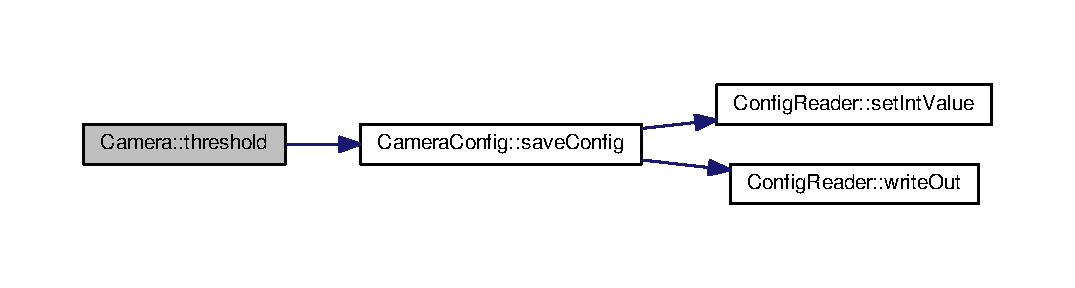
\includegraphics[width=350pt]{class_camera_ad4553e7cd83dba29a3d0b1542e28c66e_cgraph}
\end{center}
\end{figure}




\subsection{Member Data Documentation}
\index{Camera@{Camera}!camera@{camera}}
\index{camera@{camera}!Camera@{Camera}}
\subsubsection[{\texorpdfstring{camera}{camera}}]{\setlength{\rightskip}{0pt plus 5cm}C\+Instant\+Camera$\ast$ Camera\+::camera\hspace{0.3cm}{\ttfamily [protected]}}\hypertarget{class_camera_ade18caead38b42ad3ea4ca3816452996}{}\label{class_camera_ade18caead38b42ad3ea4ca3816452996}


The documentation for this class was generated from the following files\+:\begin{DoxyCompactItemize}
\item 
1\+\_\+\+Ball\+Tracking/\+Camera/\hyperlink{_camera_8hpp}{Camera.\+hpp}\item 
1\+\_\+\+Ball\+Tracking/\+Camera/\hyperlink{_camera_8cpp}{Camera.\+cpp}\end{DoxyCompactItemize}

\hypertarget{class_camera_config}{}\section{Camera\+Config Class Reference}
\label{class_camera_config}\index{Camera\+Config@{Camera\+Config}}


{\ttfamily \#include $<$Camera\+Config.\+hpp$>$}



Collaboration diagram for Camera\+Config\+:\nopagebreak
\begin{figure}[H]
\begin{center}
\leavevmode
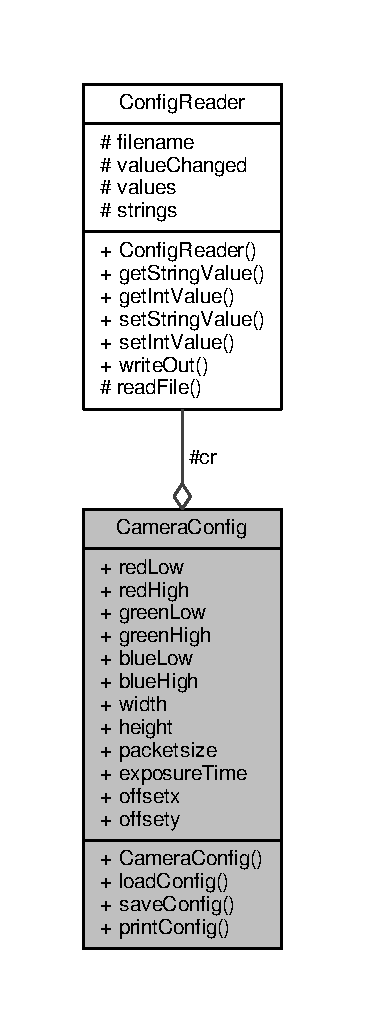
\includegraphics[width=175pt]{class_camera_config__coll__graph}
\end{center}
\end{figure}
\subsection*{Public Member Functions}
\begin{DoxyCompactItemize}
\item 
\hyperlink{class_camera_config_a03e6228afa19acfc757e310781372b6e}{Camera\+Config} ()
\item 
void \hyperlink{class_camera_config_ab8a2db9f299dc56cebcfc20b0ce72c8f}{load\+Config} ()
\item 
void \hyperlink{class_camera_config_a4c686a638a68bfa37b7490ad5fb235f6}{save\+Config} ()
\item 
void \hyperlink{class_camera_config_abc2e835a721d9724135dd88c387f2339}{print\+Config} ()
\end{DoxyCompactItemize}
\subsection*{Public Attributes}
\begin{DoxyCompactItemize}
\item 
int \hyperlink{class_camera_config_af17574ff4f72c58e893b999969be99a5}{red\+Low}
\item 
int \hyperlink{class_camera_config_a03252fbb3abecdf7d64464ec6755120b}{red\+High}
\item 
int \hyperlink{class_camera_config_ab811b83123d53257c1540414959e636e}{green\+Low}
\item 
int \hyperlink{class_camera_config_a65cee18623283080979a00c5cfdec82b}{green\+High}
\item 
int \hyperlink{class_camera_config_ab30d1064804f459fbf913367717b406e}{blue\+Low}
\item 
int \hyperlink{class_camera_config_a1d3dd499f01ce0b4be38f10c2c314ecb}{blue\+High}
\item 
int \hyperlink{class_camera_config_a96696c7f5168a06e31f46bef172d60d1}{width}
\item 
int \hyperlink{class_camera_config_a7d642c69abc40b9ca10c36c73659d08a}{height}
\item 
int \hyperlink{class_camera_config_ae3d156cca77d2082314995cd4b290f83}{packetsize}
\item 
int \hyperlink{class_camera_config_a7bde14cd01c4df4d08eba913bdc610d8}{exposure\+Time}
\item 
int \hyperlink{class_camera_config_a3a61d11401b9b2d6854f9610cdccb51f}{offsetx}
\item 
int \hyperlink{class_camera_config_a6f92a428316eec08a24a25bfdd555d37}{offsety}
\end{DoxyCompactItemize}
\subsection*{Protected Attributes}
\begin{DoxyCompactItemize}
\item 
\hyperlink{class_config_reader}{Config\+Reader} \hyperlink{class_camera_config_a9171ca2ca355b8983ec188582a2f7f8a}{cr}
\end{DoxyCompactItemize}


\subsection{Detailed Description}
\hyperlink{class_camera_config}{Camera\+Config} class 

\subsection{Constructor \& Destructor Documentation}
\index{Camera\+Config@{Camera\+Config}!Camera\+Config@{Camera\+Config}}
\index{Camera\+Config@{Camera\+Config}!Camera\+Config@{Camera\+Config}}
\subsubsection[{\texorpdfstring{Camera\+Config()}{CameraConfig()}}]{\setlength{\rightskip}{0pt plus 5cm}Camera\+Config\+::\+Camera\+Config (
\begin{DoxyParamCaption}
{}
\end{DoxyParamCaption}
)\hspace{0.3cm}{\ttfamily [inline]}}\hypertarget{class_camera_config_a03e6228afa19acfc757e310781372b6e}{}\label{class_camera_config_a03e6228afa19acfc757e310781372b6e}
\hyperlink{class_camera_config}{Camera\+Config} constructor 

Here is the call graph for this function\+:\nopagebreak
\begin{figure}[H]
\begin{center}
\leavevmode
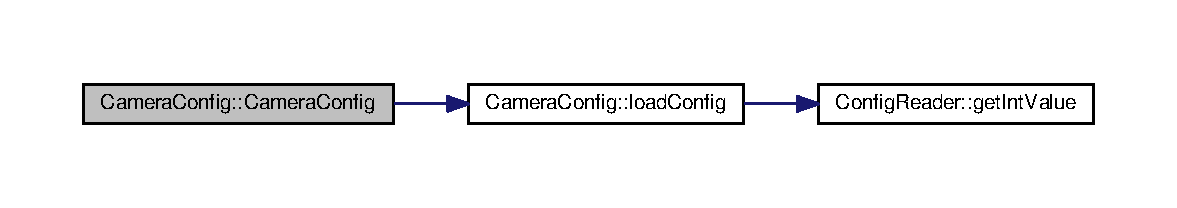
\includegraphics[width=350pt]{class_camera_config_a03e6228afa19acfc757e310781372b6e_cgraph}
\end{center}
\end{figure}




\subsection{Member Function Documentation}
\index{Camera\+Config@{Camera\+Config}!load\+Config@{load\+Config}}
\index{load\+Config@{load\+Config}!Camera\+Config@{Camera\+Config}}
\subsubsection[{\texorpdfstring{load\+Config()}{loadConfig()}}]{\setlength{\rightskip}{0pt plus 5cm}void Camera\+Config\+::load\+Config (
\begin{DoxyParamCaption}
{}
\end{DoxyParamCaption}
)\hspace{0.3cm}{\ttfamily [inline]}}\hypertarget{class_camera_config_ab8a2db9f299dc56cebcfc20b0ce72c8f}{}\label{class_camera_config_ab8a2db9f299dc56cebcfc20b0ce72c8f}
load\+Config function 

Here is the call graph for this function\+:\nopagebreak
\begin{figure}[H]
\begin{center}
\leavevmode
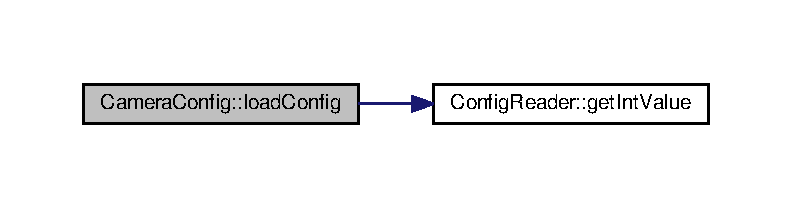
\includegraphics[width=350pt]{class_camera_config_ab8a2db9f299dc56cebcfc20b0ce72c8f_cgraph}
\end{center}
\end{figure}




Here is the caller graph for this function\+:\nopagebreak
\begin{figure}[H]
\begin{center}
\leavevmode
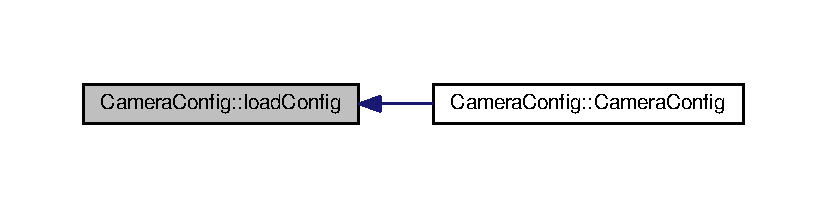
\includegraphics[width=350pt]{class_camera_config_ab8a2db9f299dc56cebcfc20b0ce72c8f_icgraph}
\end{center}
\end{figure}


\index{Camera\+Config@{Camera\+Config}!print\+Config@{print\+Config}}
\index{print\+Config@{print\+Config}!Camera\+Config@{Camera\+Config}}
\subsubsection[{\texorpdfstring{print\+Config()}{printConfig()}}]{\setlength{\rightskip}{0pt plus 5cm}void Camera\+Config\+::print\+Config (
\begin{DoxyParamCaption}
{}
\end{DoxyParamCaption}
)\hspace{0.3cm}{\ttfamily [inline]}}\hypertarget{class_camera_config_abc2e835a721d9724135dd88c387f2339}{}\label{class_camera_config_abc2e835a721d9724135dd88c387f2339}
print\+Config function \index{Camera\+Config@{Camera\+Config}!save\+Config@{save\+Config}}
\index{save\+Config@{save\+Config}!Camera\+Config@{Camera\+Config}}
\subsubsection[{\texorpdfstring{save\+Config()}{saveConfig()}}]{\setlength{\rightskip}{0pt plus 5cm}void Camera\+Config\+::save\+Config (
\begin{DoxyParamCaption}
{}
\end{DoxyParamCaption}
)\hspace{0.3cm}{\ttfamily [inline]}}\hypertarget{class_camera_config_a4c686a638a68bfa37b7490ad5fb235f6}{}\label{class_camera_config_a4c686a638a68bfa37b7490ad5fb235f6}
seva\+Config function 

Here is the call graph for this function\+:\nopagebreak
\begin{figure}[H]
\begin{center}
\leavevmode
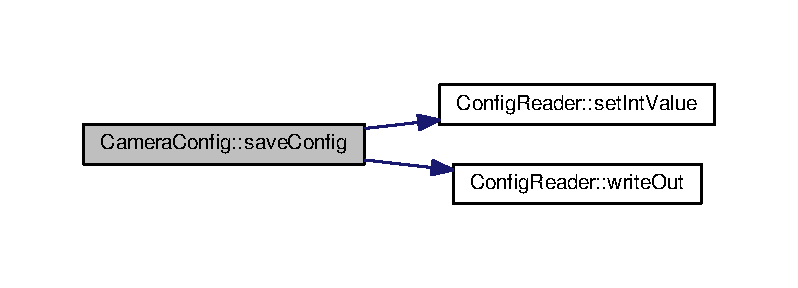
\includegraphics[width=350pt]{class_camera_config_a4c686a638a68bfa37b7490ad5fb235f6_cgraph}
\end{center}
\end{figure}




Here is the caller graph for this function\+:\nopagebreak
\begin{figure}[H]
\begin{center}
\leavevmode
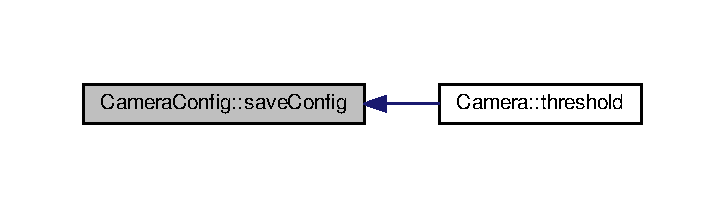
\includegraphics[width=348pt]{class_camera_config_a4c686a638a68bfa37b7490ad5fb235f6_icgraph}
\end{center}
\end{figure}




\subsection{Member Data Documentation}
\index{Camera\+Config@{Camera\+Config}!blue\+High@{blue\+High}}
\index{blue\+High@{blue\+High}!Camera\+Config@{Camera\+Config}}
\subsubsection[{\texorpdfstring{blue\+High}{blueHigh}}]{\setlength{\rightskip}{0pt plus 5cm}int Camera\+Config\+::blue\+High}\hypertarget{class_camera_config_a1d3dd499f01ce0b4be38f10c2c314ecb}{}\label{class_camera_config_a1d3dd499f01ce0b4be38f10c2c314ecb}
\index{Camera\+Config@{Camera\+Config}!blue\+Low@{blue\+Low}}
\index{blue\+Low@{blue\+Low}!Camera\+Config@{Camera\+Config}}
\subsubsection[{\texorpdfstring{blue\+Low}{blueLow}}]{\setlength{\rightskip}{0pt plus 5cm}int Camera\+Config\+::blue\+Low}\hypertarget{class_camera_config_ab30d1064804f459fbf913367717b406e}{}\label{class_camera_config_ab30d1064804f459fbf913367717b406e}
\index{Camera\+Config@{Camera\+Config}!cr@{cr}}
\index{cr@{cr}!Camera\+Config@{Camera\+Config}}
\subsubsection[{\texorpdfstring{cr}{cr}}]{\setlength{\rightskip}{0pt plus 5cm}{\bf Config\+Reader} Camera\+Config\+::cr\hspace{0.3cm}{\ttfamily [protected]}}\hypertarget{class_camera_config_a9171ca2ca355b8983ec188582a2f7f8a}{}\label{class_camera_config_a9171ca2ca355b8983ec188582a2f7f8a}
\index{Camera\+Config@{Camera\+Config}!exposure\+Time@{exposure\+Time}}
\index{exposure\+Time@{exposure\+Time}!Camera\+Config@{Camera\+Config}}
\subsubsection[{\texorpdfstring{exposure\+Time}{exposureTime}}]{\setlength{\rightskip}{0pt plus 5cm}int Camera\+Config\+::exposure\+Time}\hypertarget{class_camera_config_a7bde14cd01c4df4d08eba913bdc610d8}{}\label{class_camera_config_a7bde14cd01c4df4d08eba913bdc610d8}
\index{Camera\+Config@{Camera\+Config}!green\+High@{green\+High}}
\index{green\+High@{green\+High}!Camera\+Config@{Camera\+Config}}
\subsubsection[{\texorpdfstring{green\+High}{greenHigh}}]{\setlength{\rightskip}{0pt plus 5cm}int Camera\+Config\+::green\+High}\hypertarget{class_camera_config_a65cee18623283080979a00c5cfdec82b}{}\label{class_camera_config_a65cee18623283080979a00c5cfdec82b}
\index{Camera\+Config@{Camera\+Config}!green\+Low@{green\+Low}}
\index{green\+Low@{green\+Low}!Camera\+Config@{Camera\+Config}}
\subsubsection[{\texorpdfstring{green\+Low}{greenLow}}]{\setlength{\rightskip}{0pt plus 5cm}int Camera\+Config\+::green\+Low}\hypertarget{class_camera_config_ab811b83123d53257c1540414959e636e}{}\label{class_camera_config_ab811b83123d53257c1540414959e636e}
\index{Camera\+Config@{Camera\+Config}!height@{height}}
\index{height@{height}!Camera\+Config@{Camera\+Config}}
\subsubsection[{\texorpdfstring{height}{height}}]{\setlength{\rightskip}{0pt plus 5cm}int Camera\+Config\+::height}\hypertarget{class_camera_config_a7d642c69abc40b9ca10c36c73659d08a}{}\label{class_camera_config_a7d642c69abc40b9ca10c36c73659d08a}
\index{Camera\+Config@{Camera\+Config}!offsetx@{offsetx}}
\index{offsetx@{offsetx}!Camera\+Config@{Camera\+Config}}
\subsubsection[{\texorpdfstring{offsetx}{offsetx}}]{\setlength{\rightskip}{0pt plus 5cm}int Camera\+Config\+::offsetx}\hypertarget{class_camera_config_a3a61d11401b9b2d6854f9610cdccb51f}{}\label{class_camera_config_a3a61d11401b9b2d6854f9610cdccb51f}
\index{Camera\+Config@{Camera\+Config}!offsety@{offsety}}
\index{offsety@{offsety}!Camera\+Config@{Camera\+Config}}
\subsubsection[{\texorpdfstring{offsety}{offsety}}]{\setlength{\rightskip}{0pt plus 5cm}int Camera\+Config\+::offsety}\hypertarget{class_camera_config_a6f92a428316eec08a24a25bfdd555d37}{}\label{class_camera_config_a6f92a428316eec08a24a25bfdd555d37}
\index{Camera\+Config@{Camera\+Config}!packetsize@{packetsize}}
\index{packetsize@{packetsize}!Camera\+Config@{Camera\+Config}}
\subsubsection[{\texorpdfstring{packetsize}{packetsize}}]{\setlength{\rightskip}{0pt plus 5cm}int Camera\+Config\+::packetsize}\hypertarget{class_camera_config_ae3d156cca77d2082314995cd4b290f83}{}\label{class_camera_config_ae3d156cca77d2082314995cd4b290f83}
\index{Camera\+Config@{Camera\+Config}!red\+High@{red\+High}}
\index{red\+High@{red\+High}!Camera\+Config@{Camera\+Config}}
\subsubsection[{\texorpdfstring{red\+High}{redHigh}}]{\setlength{\rightskip}{0pt plus 5cm}int Camera\+Config\+::red\+High}\hypertarget{class_camera_config_a03252fbb3abecdf7d64464ec6755120b}{}\label{class_camera_config_a03252fbb3abecdf7d64464ec6755120b}
\index{Camera\+Config@{Camera\+Config}!red\+Low@{red\+Low}}
\index{red\+Low@{red\+Low}!Camera\+Config@{Camera\+Config}}
\subsubsection[{\texorpdfstring{red\+Low}{redLow}}]{\setlength{\rightskip}{0pt plus 5cm}int Camera\+Config\+::red\+Low}\hypertarget{class_camera_config_af17574ff4f72c58e893b999969be99a5}{}\label{class_camera_config_af17574ff4f72c58e893b999969be99a5}
\index{Camera\+Config@{Camera\+Config}!width@{width}}
\index{width@{width}!Camera\+Config@{Camera\+Config}}
\subsubsection[{\texorpdfstring{width}{width}}]{\setlength{\rightskip}{0pt plus 5cm}int Camera\+Config\+::width}\hypertarget{class_camera_config_a96696c7f5168a06e31f46bef172d60d1}{}\label{class_camera_config_a96696c7f5168a06e31f46bef172d60d1}


The documentation for this class was generated from the following file\+:\begin{DoxyCompactItemize}
\item 
Kick\+I\+T@\+Eclipse/5\+\_\+\+Data\+Type/\hyperlink{_camera_config_8hpp}{Camera\+Config.\+hpp}\end{DoxyCompactItemize}

\hypertarget{class_camera_interface}{}\section{Camera\+Interface Class Reference}
\label{class_camera_interface}\index{Camera\+Interface@{Camera\+Interface}}


{\ttfamily \#include $<$\+\_\+\+Camera\+Interface.\+hpp$>$}



Inheritance diagram for Camera\+Interface\+:\nopagebreak
\begin{figure}[H]
\begin{center}
\leavevmode
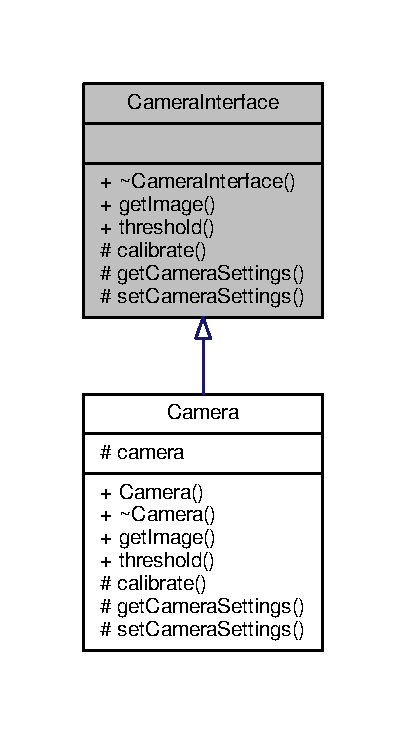
\includegraphics[width=195pt]{class_camera_interface__inherit__graph}
\end{center}
\end{figure}


Collaboration diagram for Camera\+Interface\+:\nopagebreak
\begin{figure}[H]
\begin{center}
\leavevmode
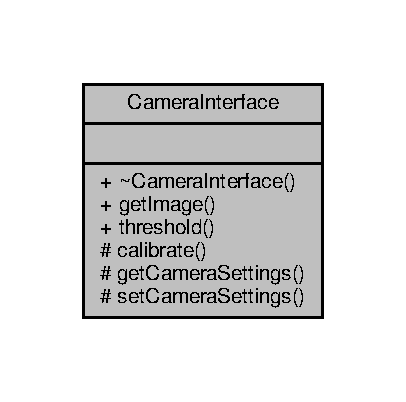
\includegraphics[width=195pt]{class_camera_interface__coll__graph}
\end{center}
\end{figure}
\subsection*{Public Member Functions}
\begin{DoxyCompactItemize}
\item 
virtual \hyperlink{class_camera_interface_a0d35ffb2f10955724043a9b8c69e30a8}{$\sim$\+Camera\+Interface} ()
\item 
virtual cv\+::\+Mat $\ast$ \hyperlink{class_camera_interface_a6e2e28f113f9db832f0e26c6c9c2a65e}{get\+Image} ()=0
\item 
virtual \hyperlink{class_camera_config}{Camera\+Config} $\ast$ \hyperlink{class_camera_interface_ae0181e4f80b465dfdf5971175fd0c497}{threshold} ()=0
\end{DoxyCompactItemize}
\subsection*{Protected Member Functions}
\begin{DoxyCompactItemize}
\item 
virtual void \hyperlink{class_camera_interface_aba26bdb1e274ed311e2a5492df576f43}{calibrate} ()=0
\item 
virtual void \hyperlink{class_camera_interface_af2abfcc95ea81477abbd0e9c4658b710}{get\+Camera\+Settings} ()=0
\item 
virtual void \hyperlink{class_camera_interface_a24463ab994557f188a86e4f2299c7404}{set\+Camera\+Settings} ()=0
\end{DoxyCompactItemize}


\subsection{Detailed Description}
\hyperlink{class_camera_interface}{Camera\+Interface} class 

\subsection{Constructor \& Destructor Documentation}
\index{Camera\+Interface@{Camera\+Interface}!````~Camera\+Interface@{$\sim$\+Camera\+Interface}}
\index{````~Camera\+Interface@{$\sim$\+Camera\+Interface}!Camera\+Interface@{Camera\+Interface}}
\subsubsection[{\texorpdfstring{$\sim$\+Camera\+Interface()}{~CameraInterface()}}]{\setlength{\rightskip}{0pt plus 5cm}virtual Camera\+Interface\+::$\sim$\+Camera\+Interface (
\begin{DoxyParamCaption}
{}
\end{DoxyParamCaption}
)\hspace{0.3cm}{\ttfamily [inline]}, {\ttfamily [virtual]}}\hypertarget{class_camera_interface_a0d35ffb2f10955724043a9b8c69e30a8}{}\label{class_camera_interface_a0d35ffb2f10955724043a9b8c69e30a8}
\hyperlink{class_camera_interface}{Camera\+Interface} destructor 

\subsection{Member Function Documentation}
\index{Camera\+Interface@{Camera\+Interface}!calibrate@{calibrate}}
\index{calibrate@{calibrate}!Camera\+Interface@{Camera\+Interface}}
\subsubsection[{\texorpdfstring{calibrate()=0}{calibrate()=0}}]{\setlength{\rightskip}{0pt plus 5cm}virtual void Camera\+Interface\+::calibrate (
\begin{DoxyParamCaption}
{}
\end{DoxyParamCaption}
)\hspace{0.3cm}{\ttfamily [protected]}, {\ttfamily [pure virtual]}}\hypertarget{class_camera_interface_aba26bdb1e274ed311e2a5492df576f43}{}\label{class_camera_interface_aba26bdb1e274ed311e2a5492df576f43}
calibrate function 

Implemented in \hyperlink{class_camera_aff4f0478ef6ed7b35f353a6d055f0481}{Camera}.

\index{Camera\+Interface@{Camera\+Interface}!get\+Camera\+Settings@{get\+Camera\+Settings}}
\index{get\+Camera\+Settings@{get\+Camera\+Settings}!Camera\+Interface@{Camera\+Interface}}
\subsubsection[{\texorpdfstring{get\+Camera\+Settings()=0}{getCameraSettings()=0}}]{\setlength{\rightskip}{0pt plus 5cm}virtual void Camera\+Interface\+::get\+Camera\+Settings (
\begin{DoxyParamCaption}
{}
\end{DoxyParamCaption}
)\hspace{0.3cm}{\ttfamily [protected]}, {\ttfamily [pure virtual]}}\hypertarget{class_camera_interface_af2abfcc95ea81477abbd0e9c4658b710}{}\label{class_camera_interface_af2abfcc95ea81477abbd0e9c4658b710}
get\+Camera\+Settings

Function prints out the adjusted values of the camera 

Implemented in \hyperlink{class_camera_a62e9e0757dc2758b118274cfa5d56ff6}{Camera}.

\index{Camera\+Interface@{Camera\+Interface}!get\+Image@{get\+Image}}
\index{get\+Image@{get\+Image}!Camera\+Interface@{Camera\+Interface}}
\subsubsection[{\texorpdfstring{get\+Image()=0}{getImage()=0}}]{\setlength{\rightskip}{0pt plus 5cm}virtual cv\+::\+Mat$\ast$ Camera\+Interface\+::get\+Image (
\begin{DoxyParamCaption}
{}
\end{DoxyParamCaption}
)\hspace{0.3cm}{\ttfamily [pure virtual]}}\hypertarget{class_camera_interface_a6e2e28f113f9db832f0e26c6c9c2a65e}{}\label{class_camera_interface_a6e2e28f113f9db832f0e26c6c9c2a65e}
get\+Image function

Function retrieves a picture from the camera

\begin{DoxyReturn}{Returns}
An image is returned 
\end{DoxyReturn}


Implemented in \hyperlink{class_camera_a45c96b9b33d73f3a5af527de0a5b6526}{Camera}.

\index{Camera\+Interface@{Camera\+Interface}!set\+Camera\+Settings@{set\+Camera\+Settings}}
\index{set\+Camera\+Settings@{set\+Camera\+Settings}!Camera\+Interface@{Camera\+Interface}}
\subsubsection[{\texorpdfstring{set\+Camera\+Settings()=0}{setCameraSettings()=0}}]{\setlength{\rightskip}{0pt plus 5cm}virtual void Camera\+Interface\+::set\+Camera\+Settings (
\begin{DoxyParamCaption}
{}
\end{DoxyParamCaption}
)\hspace{0.3cm}{\ttfamily [protected]}, {\ttfamily [pure virtual]}}\hypertarget{class_camera_interface_a24463ab994557f188a86e4f2299c7404}{}\label{class_camera_interface_a24463ab994557f188a86e4f2299c7404}
set\+Camera\+Settings

Function for initial configuration of the camera. The settings are fetched from the Camera\+Config.\+txt and passed to the Pylon\+Viewer\+Api 

Implemented in \hyperlink{class_camera_afc0e7093a6749fa1445545cd59fca7b0}{Camera}.

\index{Camera\+Interface@{Camera\+Interface}!threshold@{threshold}}
\index{threshold@{threshold}!Camera\+Interface@{Camera\+Interface}}
\subsubsection[{\texorpdfstring{threshold()=0}{threshold()=0}}]{\setlength{\rightskip}{0pt plus 5cm}virtual {\bf Camera\+Config}$\ast$ Camera\+Interface\+::threshold (
\begin{DoxyParamCaption}
{}
\end{DoxyParamCaption}
)\hspace{0.3cm}{\ttfamily [pure virtual]}}\hypertarget{class_camera_interface_ae0181e4f80b465dfdf5971175fd0c497}{}\label{class_camera_interface_ae0181e4f80b465dfdf5971175fd0c497}
Funktion threshold

This function sets the threshold values ​​for the ball detection. These values ​​are then stored in the Camera\+Config.\+txt

\begin{DoxyReturn}{Returns}
The result of the adjustment is returned 
\end{DoxyReturn}


Implemented in \hyperlink{class_camera_ad4553e7cd83dba29a3d0b1542e28c66e}{Camera}.



The documentation for this class was generated from the following file\+:\begin{DoxyCompactItemize}
\item 
Kick\+I\+T@\+Eclipse/1\+\_\+\+Ball\+Tracking/\+Camera/\hyperlink{___camera_interface_8hpp}{\+\_\+\+Camera\+Interface.\+hpp}\end{DoxyCompactItemize}

\hypertarget{class_cannot_open_config_file_exception}{}\section{Cannot\+Open\+Config\+File\+Exception Class Reference}
\label{class_cannot_open_config_file_exception}\index{Cannot\+Open\+Config\+File\+Exception@{Cannot\+Open\+Config\+File\+Exception}}


{\ttfamily \#include $<$Config\+Reader.\+hpp$>$}



Inheritance diagram for Cannot\+Open\+Config\+File\+Exception\+:\nopagebreak
\begin{figure}[H]
\begin{center}
\leavevmode
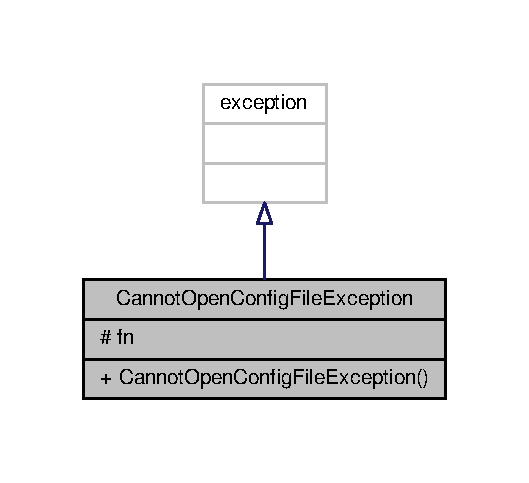
\includegraphics[width=254pt]{class_cannot_open_config_file_exception__inherit__graph}
\end{center}
\end{figure}


Collaboration diagram for Cannot\+Open\+Config\+File\+Exception\+:\nopagebreak
\begin{figure}[H]
\begin{center}
\leavevmode
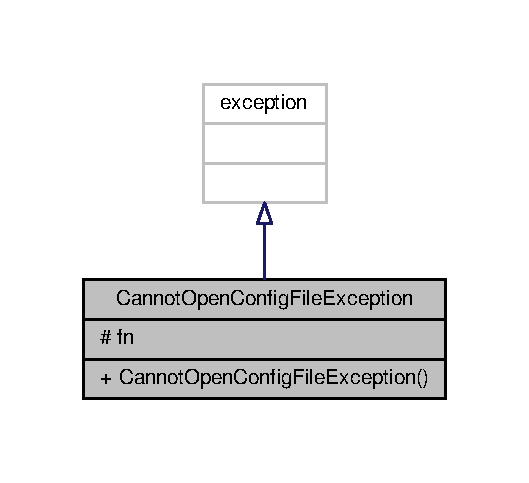
\includegraphics[width=254pt]{class_cannot_open_config_file_exception__coll__graph}
\end{center}
\end{figure}
\subsection*{Public Member Functions}
\begin{DoxyCompactItemize}
\item 
\hyperlink{class_cannot_open_config_file_exception_a16f23fec412b6c032c99dd9dac3a2f84}{Cannot\+Open\+Config\+File\+Exception} (const char $\ast$filename)
\end{DoxyCompactItemize}
\subsection*{Protected Attributes}
\begin{DoxyCompactItemize}
\item 
std\+::string \hyperlink{class_cannot_open_config_file_exception_afa011be333c848ca42ad2aa4449cddce}{fn}
\end{DoxyCompactItemize}


\subsection{Detailed Description}
\hyperlink{class_cannot_open_config_file_exception}{Cannot\+Open\+Config\+File\+Exception} class 

\subsection{Constructor \& Destructor Documentation}
\index{Cannot\+Open\+Config\+File\+Exception@{Cannot\+Open\+Config\+File\+Exception}!Cannot\+Open\+Config\+File\+Exception@{Cannot\+Open\+Config\+File\+Exception}}
\index{Cannot\+Open\+Config\+File\+Exception@{Cannot\+Open\+Config\+File\+Exception}!Cannot\+Open\+Config\+File\+Exception@{Cannot\+Open\+Config\+File\+Exception}}
\subsubsection[{\texorpdfstring{Cannot\+Open\+Config\+File\+Exception(const char $\ast$filename)}{CannotOpenConfigFileException(const char *filename)}}]{\setlength{\rightskip}{0pt plus 5cm}Cannot\+Open\+Config\+File\+Exception\+::\+Cannot\+Open\+Config\+File\+Exception (
\begin{DoxyParamCaption}
\item[{const char $\ast$}]{filename}
\end{DoxyParamCaption}
)\hspace{0.3cm}{\ttfamily [inline]}}\hypertarget{class_cannot_open_config_file_exception_a16f23fec412b6c032c99dd9dac3a2f84}{}\label{class_cannot_open_config_file_exception_a16f23fec412b6c032c99dd9dac3a2f84}
\hyperlink{class_cannot_open_config_file_exception}{Cannot\+Open\+Config\+File\+Exception} function 
\begin{DoxyParams}{Parameters}
{\em (const} & char$\ast$ filename)\+:fn(filename) \\
\hline
\end{DoxyParams}


\subsection{Member Data Documentation}
\index{Cannot\+Open\+Config\+File\+Exception@{Cannot\+Open\+Config\+File\+Exception}!fn@{fn}}
\index{fn@{fn}!Cannot\+Open\+Config\+File\+Exception@{Cannot\+Open\+Config\+File\+Exception}}
\subsubsection[{\texorpdfstring{fn}{fn}}]{\setlength{\rightskip}{0pt plus 5cm}std\+::string Cannot\+Open\+Config\+File\+Exception\+::fn\hspace{0.3cm}{\ttfamily [protected]}}\hypertarget{class_cannot_open_config_file_exception_afa011be333c848ca42ad2aa4449cddce}{}\label{class_cannot_open_config_file_exception_afa011be333c848ca42ad2aa4449cddce}


The documentation for this class was generated from the following file\+:\begin{DoxyCompactItemize}
\item 
4\+\_\+\+Utilities/\hyperlink{_config_reader_8hpp}{Config\+Reader.\+hpp}\end{DoxyCompactItemize}

\hypertarget{class_config_file_changed_exception}{}\section{Config\+File\+Changed\+Exception Class Reference}
\label{class_config_file_changed_exception}\index{Config\+File\+Changed\+Exception@{Config\+File\+Changed\+Exception}}


{\ttfamily \#include $<$Config\+Reader.\+hpp$>$}



Inheritance diagram for Config\+File\+Changed\+Exception\+:\nopagebreak
\begin{figure}[H]
\begin{center}
\leavevmode
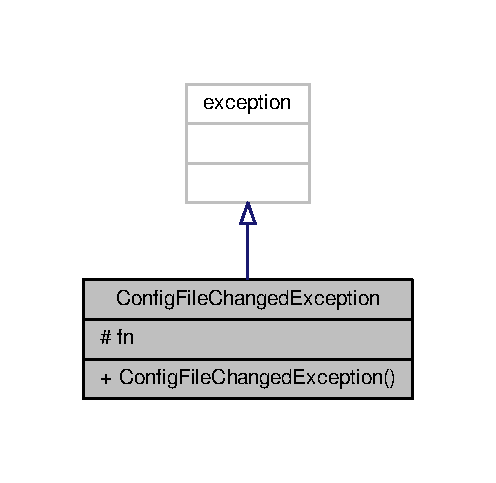
\includegraphics[width=238pt]{class_config_file_changed_exception__inherit__graph}
\end{center}
\end{figure}


Collaboration diagram for Config\+File\+Changed\+Exception\+:\nopagebreak
\begin{figure}[H]
\begin{center}
\leavevmode
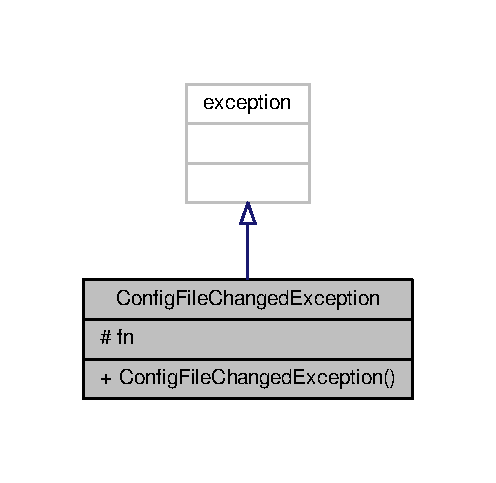
\includegraphics[width=238pt]{class_config_file_changed_exception__coll__graph}
\end{center}
\end{figure}
\subsection*{Public Member Functions}
\begin{DoxyCompactItemize}
\item 
\hyperlink{class_config_file_changed_exception_aee3967e1803eecc26850b4829a5f644b}{Config\+File\+Changed\+Exception} (const char $\ast$filename)
\end{DoxyCompactItemize}
\subsection*{Protected Attributes}
\begin{DoxyCompactItemize}
\item 
std\+::string \hyperlink{class_config_file_changed_exception_af06ed19b894876c2a61f4e6c4dee675b}{fn}
\end{DoxyCompactItemize}


\subsection{Detailed Description}
\hyperlink{class_config_file_changed_exception}{Config\+File\+Changed\+Exception} class 

\subsection{Constructor \& Destructor Documentation}
\index{Config\+File\+Changed\+Exception@{Config\+File\+Changed\+Exception}!Config\+File\+Changed\+Exception@{Config\+File\+Changed\+Exception}}
\index{Config\+File\+Changed\+Exception@{Config\+File\+Changed\+Exception}!Config\+File\+Changed\+Exception@{Config\+File\+Changed\+Exception}}
\subsubsection[{\texorpdfstring{Config\+File\+Changed\+Exception(const char $\ast$filename)}{ConfigFileChangedException(const char *filename)}}]{\setlength{\rightskip}{0pt plus 5cm}Config\+File\+Changed\+Exception\+::\+Config\+File\+Changed\+Exception (
\begin{DoxyParamCaption}
\item[{const char $\ast$}]{filename}
\end{DoxyParamCaption}
)\hspace{0.3cm}{\ttfamily [inline]}}\hypertarget{class_config_file_changed_exception_aee3967e1803eecc26850b4829a5f644b}{}\label{class_config_file_changed_exception_aee3967e1803eecc26850b4829a5f644b}
\hyperlink{class_config_file_changed_exception}{Config\+File\+Changed\+Exception} function


\begin{DoxyParams}{Parameters}
{\em (const} & char$\ast$ filename) \\
\hline
\end{DoxyParams}


\subsection{Member Data Documentation}
\index{Config\+File\+Changed\+Exception@{Config\+File\+Changed\+Exception}!fn@{fn}}
\index{fn@{fn}!Config\+File\+Changed\+Exception@{Config\+File\+Changed\+Exception}}
\subsubsection[{\texorpdfstring{fn}{fn}}]{\setlength{\rightskip}{0pt plus 5cm}std\+::string Config\+File\+Changed\+Exception\+::fn\hspace{0.3cm}{\ttfamily [protected]}}\hypertarget{class_config_file_changed_exception_af06ed19b894876c2a61f4e6c4dee675b}{}\label{class_config_file_changed_exception_af06ed19b894876c2a61f4e6c4dee675b}


The documentation for this class was generated from the following file\+:\begin{DoxyCompactItemize}
\item 
Kick\+I\+T@\+Eclipse/4\+\_\+\+Utilities/\hyperlink{_config_reader_8hpp}{Config\+Reader.\+hpp}\end{DoxyCompactItemize}

\hypertarget{class_config_reader}{}\section{Config\+Reader Class Reference}
\label{class_config_reader}\index{Config\+Reader@{Config\+Reader}}


{\ttfamily \#include $<$Config\+Reader.\+hpp$>$}



Collaboration diagram for Config\+Reader\+:\nopagebreak
\begin{figure}[H]
\begin{center}
\leavevmode
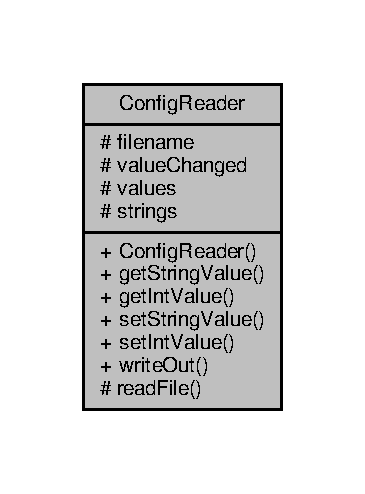
\includegraphics[width=175pt]{class_config_reader__coll__graph}
\end{center}
\end{figure}
\subsection*{Public Member Functions}
\begin{DoxyCompactItemize}
\item 
\hyperlink{class_config_reader_a4c1909efc98e8d6308c7871554f68a1a}{Config\+Reader} (const char $\ast$\hyperlink{class_config_reader_a82435410daeab9beb0dc90500976acfc}{filename})
\item 
std\+::string \hyperlink{class_config_reader_a94455bd2a38611704e4b4523b5be538c}{get\+String\+Value} (const char $\ast$name)
\item 
int \hyperlink{class_config_reader_a6843a6aecc2bc7115d1052bafb77df80}{get\+Int\+Value} (const char $\ast$name)
\item 
void \hyperlink{class_config_reader_a91fbf7d656050bd20f17075f6e8c6304}{set\+String\+Value} (const char $\ast$name, const char $\ast$value)
\item 
void \hyperlink{class_config_reader_a82d8f2ba319008e3479f2b4d0b80592a}{set\+Int\+Value} (const char $\ast$name, const int value)
\item 
void \hyperlink{class_config_reader_a40c8fc72bb2a097398c821cfec78ba6e}{write\+Out} ()
\end{DoxyCompactItemize}
\subsection*{Protected Member Functions}
\begin{DoxyCompactItemize}
\item 
void \hyperlink{class_config_reader_a9a984c109425eecf599f606f10a2948c}{read\+File} ()
\end{DoxyCompactItemize}
\subsection*{Protected Attributes}
\begin{DoxyCompactItemize}
\item 
const char $\ast$ \hyperlink{class_config_reader_a82435410daeab9beb0dc90500976acfc}{filename}
\item 
bool \hyperlink{class_config_reader_aa384495927b6c1677d39e34eac3e577c}{value\+Changed} = false
\item 
std\+::map$<$ std\+::string, int $>$ \hyperlink{class_config_reader_ad7bd3a0ec9513b9f385a658752c87b37}{values}
\item 
std\+::map$<$ std\+::string, std\+::string $>$ \hyperlink{class_config_reader_ac03a3baf208f4dd2c2e5a8c9494b431b}{strings}
\end{DoxyCompactItemize}


\subsection{Detailed Description}
\hyperlink{class_config_reader}{Config\+Reader} class 

\subsection{Constructor \& Destructor Documentation}
\index{Config\+Reader@{Config\+Reader}!Config\+Reader@{Config\+Reader}}
\index{Config\+Reader@{Config\+Reader}!Config\+Reader@{Config\+Reader}}
\subsubsection[{\texorpdfstring{Config\+Reader(const char $\ast$filename)}{ConfigReader(const char *filename)}}]{\setlength{\rightskip}{0pt plus 5cm}Config\+Reader\+::\+Config\+Reader (
\begin{DoxyParamCaption}
\item[{const char $\ast$}]{filename}
\end{DoxyParamCaption}
)}\hypertarget{class_config_reader_a4c1909efc98e8d6308c7871554f68a1a}{}\label{class_config_reader_a4c1909efc98e8d6308c7871554f68a1a}
\hyperlink{class_config_reader}{Config\+Reader} constructor


\begin{DoxyParams}{Parameters}
{\em (const} & char$\ast$ filename) \\
\hline
\end{DoxyParams}


Here is the call graph for this function\+:\nopagebreak
\begin{figure}[H]
\begin{center}
\leavevmode
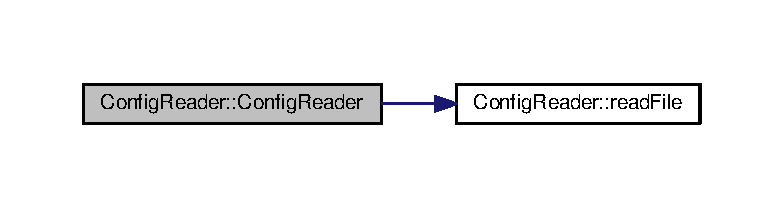
\includegraphics[width=350pt]{class_config_reader_a4c1909efc98e8d6308c7871554f68a1a_cgraph}
\end{center}
\end{figure}




\subsection{Member Function Documentation}
\index{Config\+Reader@{Config\+Reader}!get\+Int\+Value@{get\+Int\+Value}}
\index{get\+Int\+Value@{get\+Int\+Value}!Config\+Reader@{Config\+Reader}}
\subsubsection[{\texorpdfstring{get\+Int\+Value(const char $\ast$name)}{getIntValue(const char *name)}}]{\setlength{\rightskip}{0pt plus 5cm}int Config\+Reader\+::get\+Int\+Value (
\begin{DoxyParamCaption}
\item[{const char $\ast$}]{name}
\end{DoxyParamCaption}
)}\hypertarget{class_config_reader_a6843a6aecc2bc7115d1052bafb77df80}{}\label{class_config_reader_a6843a6aecc2bc7115d1052bafb77df80}
get\+Int\+Value function

Throws \hyperlink{class_parameter_not_found_exception}{Parameter\+Not\+Found\+Exception} if the parameter cannot be found.


\begin{DoxyParams}{Parameters}
{\em (const} & char$\ast$ name) \\
\hline
\end{DoxyParams}


Here is the caller graph for this function\+:\nopagebreak
\begin{figure}[H]
\begin{center}
\leavevmode
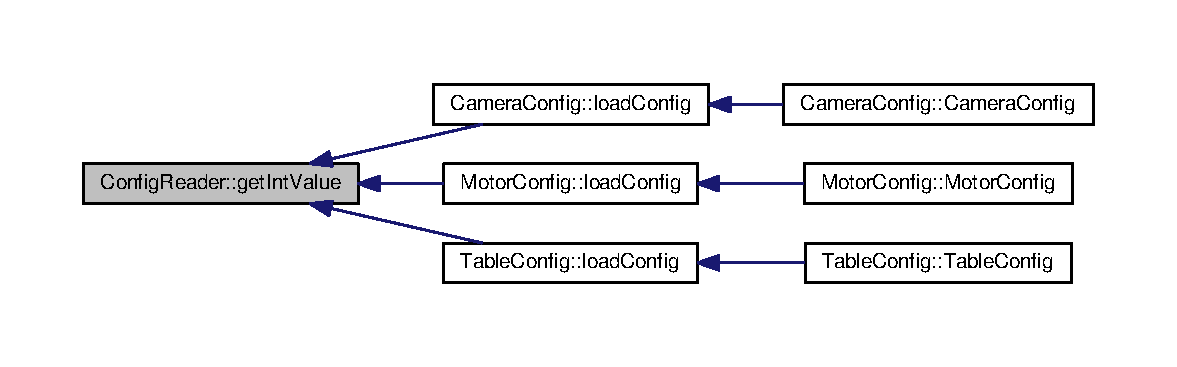
\includegraphics[width=350pt]{class_config_reader_a6843a6aecc2bc7115d1052bafb77df80_icgraph}
\end{center}
\end{figure}


\index{Config\+Reader@{Config\+Reader}!get\+String\+Value@{get\+String\+Value}}
\index{get\+String\+Value@{get\+String\+Value}!Config\+Reader@{Config\+Reader}}
\subsubsection[{\texorpdfstring{get\+String\+Value(const char $\ast$name)}{getStringValue(const char *name)}}]{\setlength{\rightskip}{0pt plus 5cm}std\+::string Config\+Reader\+::get\+String\+Value (
\begin{DoxyParamCaption}
\item[{const char $\ast$}]{name}
\end{DoxyParamCaption}
)}\hypertarget{class_config_reader_a94455bd2a38611704e4b4523b5be538c}{}\label{class_config_reader_a94455bd2a38611704e4b4523b5be538c}
get\+String\+Value function

Throws \hyperlink{class_parameter_not_found_exception}{Parameter\+Not\+Found\+Exception} if the parameter cannot be found.


\begin{DoxyParams}{Parameters}
{\em (const} & char$\ast$ name) \\
\hline
\end{DoxyParams}


Here is the caller graph for this function\+:\nopagebreak
\begin{figure}[H]
\begin{center}
\leavevmode
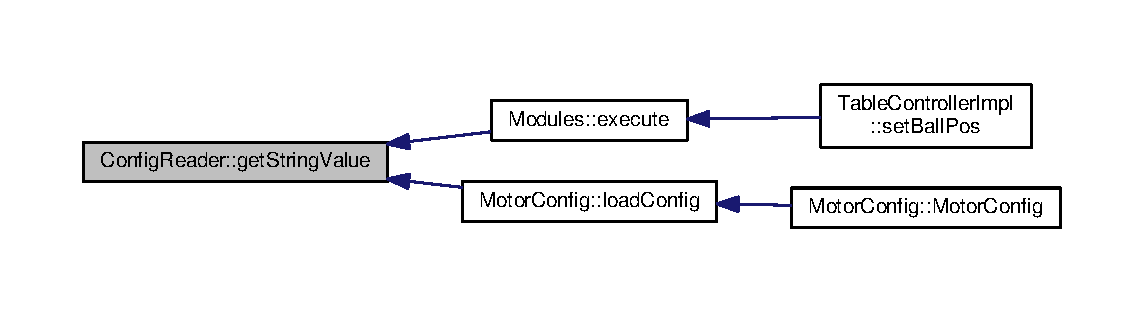
\includegraphics[width=350pt]{class_config_reader_a94455bd2a38611704e4b4523b5be538c_icgraph}
\end{center}
\end{figure}


\index{Config\+Reader@{Config\+Reader}!read\+File@{read\+File}}
\index{read\+File@{read\+File}!Config\+Reader@{Config\+Reader}}
\subsubsection[{\texorpdfstring{read\+File()}{readFile()}}]{\setlength{\rightskip}{0pt plus 5cm}void Config\+Reader\+::read\+File (
\begin{DoxyParamCaption}
{}
\end{DoxyParamCaption}
)\hspace{0.3cm}{\ttfamily [protected]}}\hypertarget{class_config_reader_a9a984c109425eecf599f606f10a2948c}{}\label{class_config_reader_a9a984c109425eecf599f606f10a2948c}
read\+File function 

Here is the caller graph for this function\+:\nopagebreak
\begin{figure}[H]
\begin{center}
\leavevmode
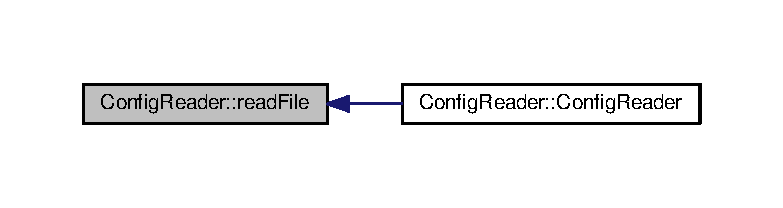
\includegraphics[width=350pt]{class_config_reader_a9a984c109425eecf599f606f10a2948c_icgraph}
\end{center}
\end{figure}


\index{Config\+Reader@{Config\+Reader}!set\+Int\+Value@{set\+Int\+Value}}
\index{set\+Int\+Value@{set\+Int\+Value}!Config\+Reader@{Config\+Reader}}
\subsubsection[{\texorpdfstring{set\+Int\+Value(const char $\ast$name, const int value)}{setIntValue(const char *name, const int value)}}]{\setlength{\rightskip}{0pt plus 5cm}void Config\+Reader\+::set\+Int\+Value (
\begin{DoxyParamCaption}
\item[{const char $\ast$}]{name, }
\item[{const int}]{value}
\end{DoxyParamCaption}
)}\hypertarget{class_config_reader_a82d8f2ba319008e3479f2b4d0b80592a}{}\label{class_config_reader_a82d8f2ba319008e3479f2b4d0b80592a}
set\+Int\+Value function

Function to update a value. If the value doesn\textquotesingle{}t exist yet, it will be added to the data set.


\begin{DoxyParams}{Parameters}
{\em (const} & char$\ast$ name, const int value) \\
\hline
\end{DoxyParams}


Here is the caller graph for this function\+:\nopagebreak
\begin{figure}[H]
\begin{center}
\leavevmode
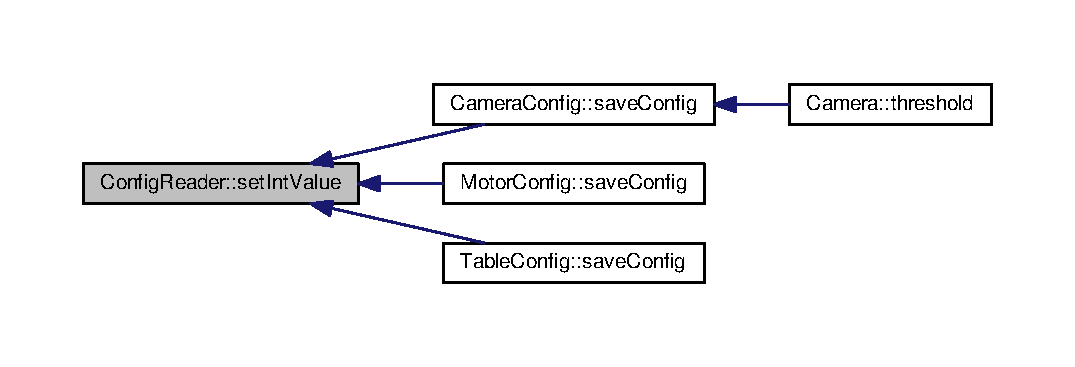
\includegraphics[width=350pt]{class_config_reader_a82d8f2ba319008e3479f2b4d0b80592a_icgraph}
\end{center}
\end{figure}


\index{Config\+Reader@{Config\+Reader}!set\+String\+Value@{set\+String\+Value}}
\index{set\+String\+Value@{set\+String\+Value}!Config\+Reader@{Config\+Reader}}
\subsubsection[{\texorpdfstring{set\+String\+Value(const char $\ast$name, const char $\ast$value)}{setStringValue(const char *name, const char *value)}}]{\setlength{\rightskip}{0pt plus 5cm}void Config\+Reader\+::set\+String\+Value (
\begin{DoxyParamCaption}
\item[{const char $\ast$}]{name, }
\item[{const char $\ast$}]{value}
\end{DoxyParamCaption}
)}\hypertarget{class_config_reader_a91fbf7d656050bd20f17075f6e8c6304}{}\label{class_config_reader_a91fbf7d656050bd20f17075f6e8c6304}
set\+String\+Value function

Function to update a value. If the value doesn\textquotesingle{}t exist yet, it will be added to the data set.


\begin{DoxyParams}{Parameters}
{\em (const} & char$\ast$ name, const char$\ast$ value) \\
\hline
\end{DoxyParams}


Here is the caller graph for this function\+:\nopagebreak
\begin{figure}[H]
\begin{center}
\leavevmode
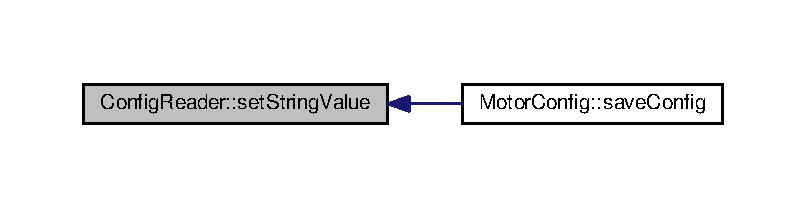
\includegraphics[width=350pt]{class_config_reader_a91fbf7d656050bd20f17075f6e8c6304_icgraph}
\end{center}
\end{figure}


\index{Config\+Reader@{Config\+Reader}!write\+Out@{write\+Out}}
\index{write\+Out@{write\+Out}!Config\+Reader@{Config\+Reader}}
\subsubsection[{\texorpdfstring{write\+Out()}{writeOut()}}]{\setlength{\rightskip}{0pt plus 5cm}void Config\+Reader\+::write\+Out (
\begin{DoxyParamCaption}
{}
\end{DoxyParamCaption}
)}\hypertarget{class_config_reader_a40c8fc72bb2a097398c821cfec78ba6e}{}\label{class_config_reader_a40c8fc72bb2a097398c821cfec78ba6e}
write\+Out function

Function to rewrite the file in case that any of the values have changed. 

Here is the caller graph for this function\+:\nopagebreak
\begin{figure}[H]
\begin{center}
\leavevmode
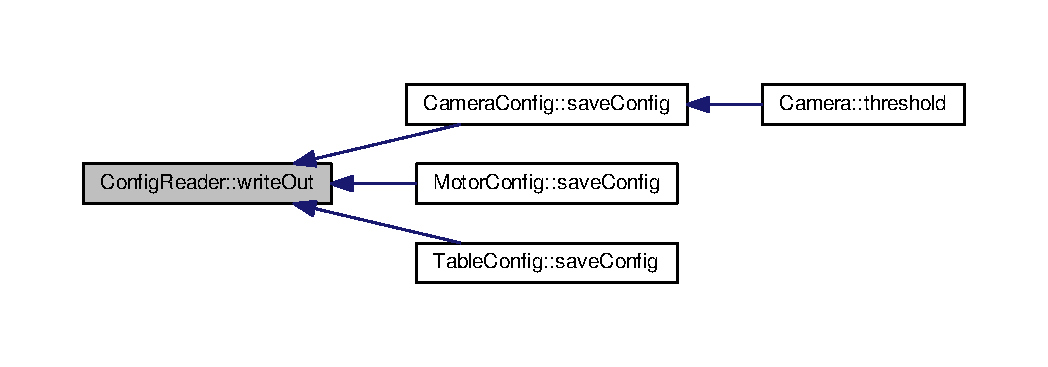
\includegraphics[width=350pt]{class_config_reader_a40c8fc72bb2a097398c821cfec78ba6e_icgraph}
\end{center}
\end{figure}




\subsection{Member Data Documentation}
\index{Config\+Reader@{Config\+Reader}!filename@{filename}}
\index{filename@{filename}!Config\+Reader@{Config\+Reader}}
\subsubsection[{\texorpdfstring{filename}{filename}}]{\setlength{\rightskip}{0pt plus 5cm}const char$\ast$ Config\+Reader\+::filename\hspace{0.3cm}{\ttfamily [protected]}}\hypertarget{class_config_reader_a82435410daeab9beb0dc90500976acfc}{}\label{class_config_reader_a82435410daeab9beb0dc90500976acfc}
\index{Config\+Reader@{Config\+Reader}!strings@{strings}}
\index{strings@{strings}!Config\+Reader@{Config\+Reader}}
\subsubsection[{\texorpdfstring{strings}{strings}}]{\setlength{\rightskip}{0pt plus 5cm}std\+::map$<$std\+::string, std\+::string$>$ Config\+Reader\+::strings\hspace{0.3cm}{\ttfamily [protected]}}\hypertarget{class_config_reader_ac03a3baf208f4dd2c2e5a8c9494b431b}{}\label{class_config_reader_ac03a3baf208f4dd2c2e5a8c9494b431b}
\index{Config\+Reader@{Config\+Reader}!value\+Changed@{value\+Changed}}
\index{value\+Changed@{value\+Changed}!Config\+Reader@{Config\+Reader}}
\subsubsection[{\texorpdfstring{value\+Changed}{valueChanged}}]{\setlength{\rightskip}{0pt plus 5cm}bool Config\+Reader\+::value\+Changed = false\hspace{0.3cm}{\ttfamily [protected]}}\hypertarget{class_config_reader_aa384495927b6c1677d39e34eac3e577c}{}\label{class_config_reader_aa384495927b6c1677d39e34eac3e577c}
\index{Config\+Reader@{Config\+Reader}!values@{values}}
\index{values@{values}!Config\+Reader@{Config\+Reader}}
\subsubsection[{\texorpdfstring{values}{values}}]{\setlength{\rightskip}{0pt plus 5cm}std\+::map$<$std\+::string, int$>$ Config\+Reader\+::values\hspace{0.3cm}{\ttfamily [protected]}}\hypertarget{class_config_reader_ad7bd3a0ec9513b9f385a658752c87b37}{}\label{class_config_reader_ad7bd3a0ec9513b9f385a658752c87b37}


The documentation for this class was generated from the following files\+:\begin{DoxyCompactItemize}
\item 
Kick\+I\+T@\+Eclipse/4\+\_\+\+Utilities/\hyperlink{_config_reader_8hpp}{Config\+Reader.\+hpp}\item 
Kick\+I\+T@\+Eclipse/4\+\_\+\+Utilities/\hyperlink{_config_reader_8cpp}{Config\+Reader.\+cpp}\end{DoxyCompactItemize}

\hypertarget{class_function_allready_registered}{}\section{Function\+Allready\+Registered Class Reference}
\label{class_function_allready_registered}\index{Function\+Allready\+Registered@{Function\+Allready\+Registered}}


{\ttfamily \#include $<$Modules.\+hpp$>$}



Inheritance diagram for Function\+Allready\+Registered\+:\nopagebreak
\begin{figure}[H]
\begin{center}
\leavevmode
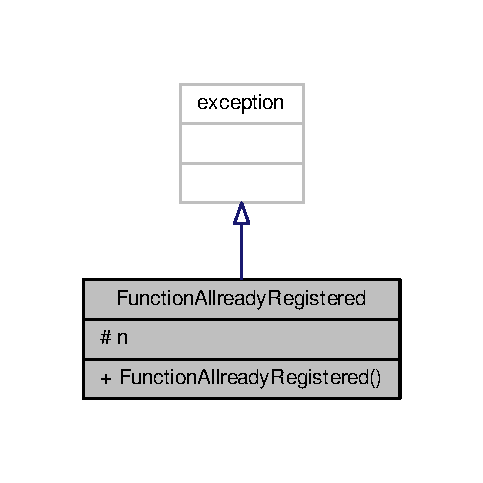
\includegraphics[width=232pt]{class_function_allready_registered__inherit__graph}
\end{center}
\end{figure}


Collaboration diagram for Function\+Allready\+Registered\+:\nopagebreak
\begin{figure}[H]
\begin{center}
\leavevmode
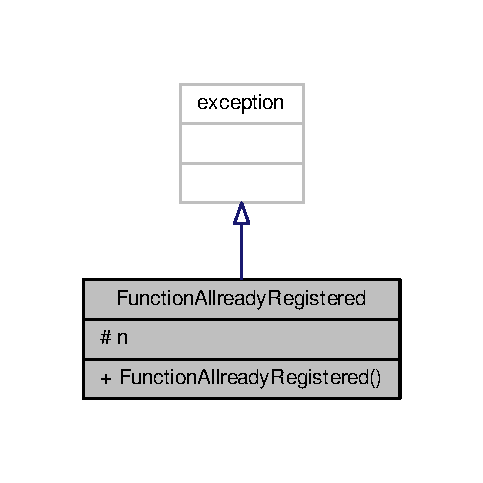
\includegraphics[width=232pt]{class_function_allready_registered__coll__graph}
\end{center}
\end{figure}
\subsection*{Public Member Functions}
\begin{DoxyCompactItemize}
\item 
\hyperlink{class_function_allready_registered_ae47ae32e5f31be4796ed5267717bc53a}{Function\+Allready\+Registered} (const char $\ast$name)
\end{DoxyCompactItemize}
\subsection*{Protected Attributes}
\begin{DoxyCompactItemize}
\item 
std\+::string \hyperlink{class_function_allready_registered_aa76fa85233839b55de8ce0d1f0201933}{n}
\end{DoxyCompactItemize}


\subsection{Detailed Description}
\hyperlink{class_function_allready_registered}{Function\+Allready\+Registered} class 

\subsection{Constructor \& Destructor Documentation}
\index{Function\+Allready\+Registered@{Function\+Allready\+Registered}!Function\+Allready\+Registered@{Function\+Allready\+Registered}}
\index{Function\+Allready\+Registered@{Function\+Allready\+Registered}!Function\+Allready\+Registered@{Function\+Allready\+Registered}}
\subsubsection[{\texorpdfstring{Function\+Allready\+Registered(const char $\ast$name)}{FunctionAllreadyRegistered(const char *name)}}]{\setlength{\rightskip}{0pt plus 5cm}Function\+Allready\+Registered\+::\+Function\+Allready\+Registered (
\begin{DoxyParamCaption}
\item[{const char $\ast$}]{name}
\end{DoxyParamCaption}
)\hspace{0.3cm}{\ttfamily [inline]}}\hypertarget{class_function_allready_registered_ae47ae32e5f31be4796ed5267717bc53a}{}\label{class_function_allready_registered_ae47ae32e5f31be4796ed5267717bc53a}
\hyperlink{class_function_allready_registered}{Function\+Allready\+Registered} function 

\subsection{Member Data Documentation}
\index{Function\+Allready\+Registered@{Function\+Allready\+Registered}!n@{n}}
\index{n@{n}!Function\+Allready\+Registered@{Function\+Allready\+Registered}}
\subsubsection[{\texorpdfstring{n}{n}}]{\setlength{\rightskip}{0pt plus 5cm}std\+::string Function\+Allready\+Registered\+::n\hspace{0.3cm}{\ttfamily [protected]}}\hypertarget{class_function_allready_registered_aa76fa85233839b55de8ce0d1f0201933}{}\label{class_function_allready_registered_aa76fa85233839b55de8ce0d1f0201933}


The documentation for this class was generated from the following file\+:\begin{DoxyCompactItemize}
\item 
4\+\_\+\+Utilities/\hyperlink{_modules_8hpp}{Modules.\+hpp}\end{DoxyCompactItemize}

\hypertarget{class_function_not_found_exception}{}\section{Function\+Not\+Found\+Exception Class Reference}
\label{class_function_not_found_exception}\index{Function\+Not\+Found\+Exception@{Function\+Not\+Found\+Exception}}


{\ttfamily \#include $<$Modules.\+hpp$>$}



Inheritance diagram for Function\+Not\+Found\+Exception\+:\nopagebreak
\begin{figure}[H]
\begin{center}
\leavevmode
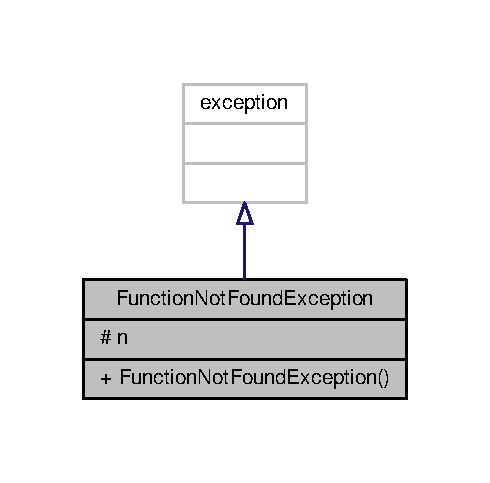
\includegraphics[width=235pt]{class_function_not_found_exception__inherit__graph}
\end{center}
\end{figure}


Collaboration diagram for Function\+Not\+Found\+Exception\+:\nopagebreak
\begin{figure}[H]
\begin{center}
\leavevmode
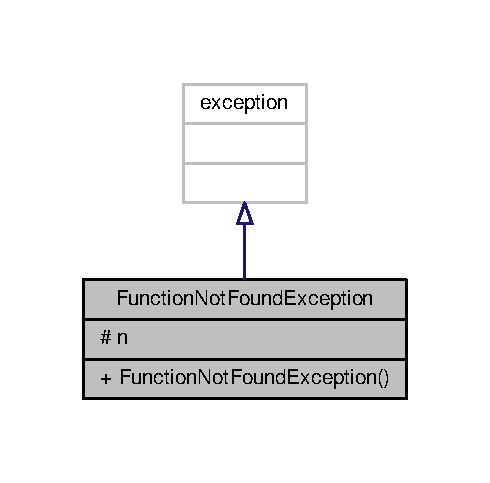
\includegraphics[width=235pt]{class_function_not_found_exception__coll__graph}
\end{center}
\end{figure}
\subsection*{Public Member Functions}
\begin{DoxyCompactItemize}
\item 
\hyperlink{class_function_not_found_exception_a7c0198d24a9f7d74d5e74c9872e6ee09}{Function\+Not\+Found\+Exception} (const char $\ast$name)
\end{DoxyCompactItemize}
\subsection*{Protected Attributes}
\begin{DoxyCompactItemize}
\item 
std\+::string \hyperlink{class_function_not_found_exception_af2547016caeac6ac3dd21f0ca070c6af}{n}
\end{DoxyCompactItemize}


\subsection{Detailed Description}
\hyperlink{class_function_not_found_exception}{Function\+Not\+Found\+Exception} class 

\subsection{Constructor \& Destructor Documentation}
\index{Function\+Not\+Found\+Exception@{Function\+Not\+Found\+Exception}!Function\+Not\+Found\+Exception@{Function\+Not\+Found\+Exception}}
\index{Function\+Not\+Found\+Exception@{Function\+Not\+Found\+Exception}!Function\+Not\+Found\+Exception@{Function\+Not\+Found\+Exception}}
\subsubsection[{\texorpdfstring{Function\+Not\+Found\+Exception(const char $\ast$name)}{FunctionNotFoundException(const char *name)}}]{\setlength{\rightskip}{0pt plus 5cm}Function\+Not\+Found\+Exception\+::\+Function\+Not\+Found\+Exception (
\begin{DoxyParamCaption}
\item[{const char $\ast$}]{name}
\end{DoxyParamCaption}
)\hspace{0.3cm}{\ttfamily [inline]}}\hypertarget{class_function_not_found_exception_a7c0198d24a9f7d74d5e74c9872e6ee09}{}\label{class_function_not_found_exception_a7c0198d24a9f7d74d5e74c9872e6ee09}
\hyperlink{class_function_not_found_exception}{Function\+Not\+Found\+Exception} function 

Here is the caller graph for this function\+:\nopagebreak
\begin{figure}[H]
\begin{center}
\leavevmode
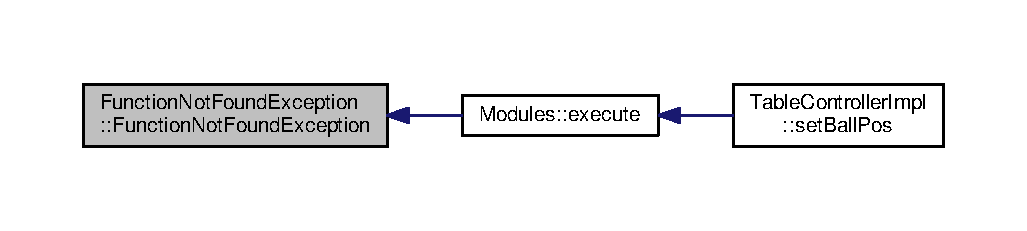
\includegraphics[width=350pt]{class_function_not_found_exception_a7c0198d24a9f7d74d5e74c9872e6ee09_icgraph}
\end{center}
\end{figure}




\subsection{Member Data Documentation}
\index{Function\+Not\+Found\+Exception@{Function\+Not\+Found\+Exception}!n@{n}}
\index{n@{n}!Function\+Not\+Found\+Exception@{Function\+Not\+Found\+Exception}}
\subsubsection[{\texorpdfstring{n}{n}}]{\setlength{\rightskip}{0pt plus 5cm}std\+::string Function\+Not\+Found\+Exception\+::n\hspace{0.3cm}{\ttfamily [protected]}}\hypertarget{class_function_not_found_exception_af2547016caeac6ac3dd21f0ca070c6af}{}\label{class_function_not_found_exception_af2547016caeac6ac3dd21f0ca070c6af}


The documentation for this class was generated from the following file\+:\begin{DoxyCompactItemize}
\item 
Kick\+I\+T@\+Eclipse/4\+\_\+\+Utilities/\hyperlink{_modules_8hpp}{Modules.\+hpp}\end{DoxyCompactItemize}

\hypertarget{class_modules}{}\section{Modules Class Reference}
\label{class_modules}\index{Modules@{Modules}}


{\ttfamily \#include $<$Modules.\+hpp$>$}



Collaboration diagram for Modules\+:\nopagebreak
\begin{figure}[H]
\begin{center}
\leavevmode
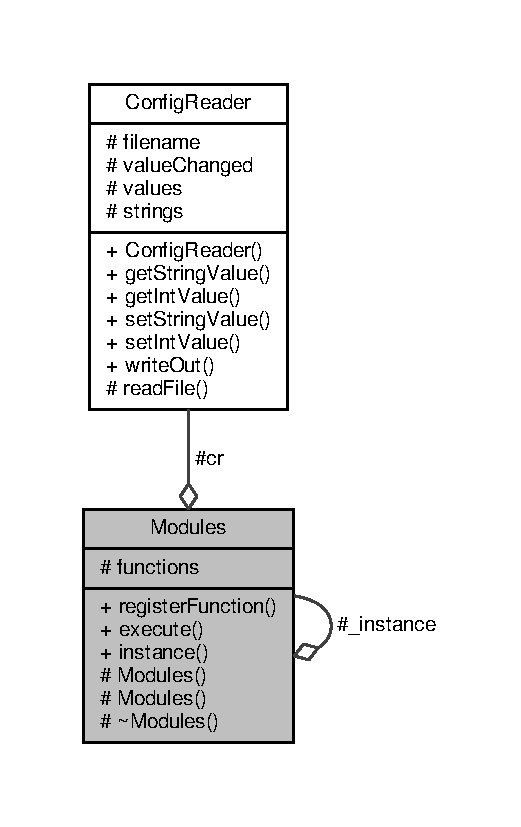
\includegraphics[width=250pt]{class_modules__coll__graph}
\end{center}
\end{figure}
\subsection*{Public Member Functions}
\begin{DoxyCompactItemize}
\item 
void \hyperlink{class_modules_a01735870f0eb88e2847a822be229f927}{register\+Function} (const char $\ast$name, \hyperlink{_modules_8hpp_ab9dff9a0870eba3247a74a386629294f}{fp} function)
\item 
void \hyperlink{class_modules_a37a7813533ef4fdce805609ace458207}{execute} (const char $\ast$algo, std\+::vector$<$ void $\ast$ $>$ $\ast$params)
\end{DoxyCompactItemize}
\subsection*{Static Public Member Functions}
\begin{DoxyCompactItemize}
\item 
static \hyperlink{class_modules}{Modules} $\ast$ \hyperlink{class_modules_a89c623a11268379d1f8516434d775460}{instance} ()
\end{DoxyCompactItemize}
\subsection*{Protected Member Functions}
\begin{DoxyCompactItemize}
\item 
\hyperlink{class_modules_a5beb72cecb96b6f1f53df16451bda24c}{Modules} ()
\item 
\hyperlink{class_modules_a48ae2b32b914d75ce26cd9886cc07ffc}{Modules} (const \hyperlink{class_modules}{Modules} \&)
\item 
\hyperlink{class_modules_a155d288c001da10d23fe918f6c065a97}{$\sim$\+Modules} ()
\end{DoxyCompactItemize}
\subsection*{Protected Attributes}
\begin{DoxyCompactItemize}
\item 
std\+::map$<$ std\+::string, \hyperlink{_modules_8hpp_ab9dff9a0870eba3247a74a386629294f}{fp} $>$ \hyperlink{class_modules_a96b175e7cd625d536d12f9c5e4aa8318}{functions}
\item 
\hyperlink{class_config_reader}{Config\+Reader} \hyperlink{class_modules_a26598b42bad97f63a6662078afb61af4}{cr}
\end{DoxyCompactItemize}
\subsection*{Static Protected Attributes}
\begin{DoxyCompactItemize}
\item 
static \hyperlink{class_modules}{Modules} $\ast$ \hyperlink{class_modules_ad82835853c834bfec3aa53da4b75def4}{\+\_\+instance} = 0
\end{DoxyCompactItemize}


\subsection{Detailed Description}
\hyperlink{class_modules}{Modules} class 

\subsection{Constructor \& Destructor Documentation}
\index{Modules@{Modules}!Modules@{Modules}}
\index{Modules@{Modules}!Modules@{Modules}}
\subsubsection[{\texorpdfstring{Modules()}{Modules()}}]{\setlength{\rightskip}{0pt plus 5cm}Modules\+::\+Modules (
\begin{DoxyParamCaption}
{}
\end{DoxyParamCaption}
)\hspace{0.3cm}{\ttfamily [inline]}, {\ttfamily [protected]}}\hypertarget{class_modules_a5beb72cecb96b6f1f53df16451bda24c}{}\label{class_modules_a5beb72cecb96b6f1f53df16451bda24c}
\hyperlink{class_modules}{Modules} constructor \index{Modules@{Modules}!Modules@{Modules}}
\index{Modules@{Modules}!Modules@{Modules}}
\subsubsection[{\texorpdfstring{Modules(const Modules \&)}{Modules(const Modules &)}}]{\setlength{\rightskip}{0pt plus 5cm}Modules\+::\+Modules (
\begin{DoxyParamCaption}
\item[{const {\bf Modules} \&}]{}
\end{DoxyParamCaption}
)\hspace{0.3cm}{\ttfamily [protected]}}\hypertarget{class_modules_a48ae2b32b914d75ce26cd9886cc07ffc}{}\label{class_modules_a48ae2b32b914d75ce26cd9886cc07ffc}
\hyperlink{class_modules}{Modules} function


\begin{DoxyParams}{Parameters}
{\em (const} & \hyperlink{class_modules}{Modules}\&) \\
\hline
\end{DoxyParams}
\index{Modules@{Modules}!````~Modules@{$\sim$\+Modules}}
\index{````~Modules@{$\sim$\+Modules}!Modules@{Modules}}
\subsubsection[{\texorpdfstring{$\sim$\+Modules()}{~Modules()}}]{\setlength{\rightskip}{0pt plus 5cm}Modules\+::$\sim$\+Modules (
\begin{DoxyParamCaption}
{}
\end{DoxyParamCaption}
)\hspace{0.3cm}{\ttfamily [inline]}, {\ttfamily [protected]}}\hypertarget{class_modules_a155d288c001da10d23fe918f6c065a97}{}\label{class_modules_a155d288c001da10d23fe918f6c065a97}
\hyperlink{class_modules}{Modules} destructor 

\subsection{Member Function Documentation}
\index{Modules@{Modules}!execute@{execute}}
\index{execute@{execute}!Modules@{Modules}}
\subsubsection[{\texorpdfstring{execute(const char $\ast$algo, std\+::vector$<$ void $\ast$ $>$ $\ast$params)}{execute(const char *algo, std::vector< void * > *params)}}]{\setlength{\rightskip}{0pt plus 5cm}void Modules\+::execute (
\begin{DoxyParamCaption}
\item[{const char $\ast$}]{algo, }
\item[{std\+::vector$<$ void $\ast$ $>$ $\ast$}]{params}
\end{DoxyParamCaption}
)\hspace{0.3cm}{\ttfamily [inline]}}\hypertarget{class_modules_a37a7813533ef4fdce805609ace458207}{}\label{class_modules_a37a7813533ef4fdce805609ace458207}
execute function


\begin{DoxyParams}{Parameters}
{\em (const} & char$\ast$ algo, vector$<$void$\ast$$>$$\ast$ params)\\
\hline
\end{DoxyParams}
Find out which function is referenced by config-\/file. Look up if that function has been registered.

Throws \hyperlink{class_function_not_found_exception}{Function\+Not\+Found\+Exception} if the name has not been registered or cannot be found in config file. 

Here is the call graph for this function\+:\nopagebreak
\begin{figure}[H]
\begin{center}
\leavevmode
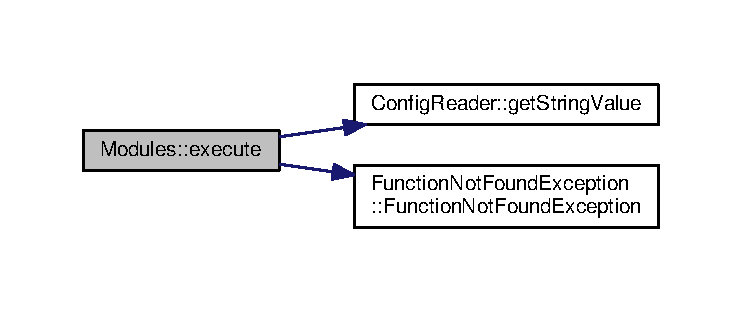
\includegraphics[width=350pt]{class_modules_a37a7813533ef4fdce805609ace458207_cgraph}
\end{center}
\end{figure}




Here is the caller graph for this function\+:\nopagebreak
\begin{figure}[H]
\begin{center}
\leavevmode
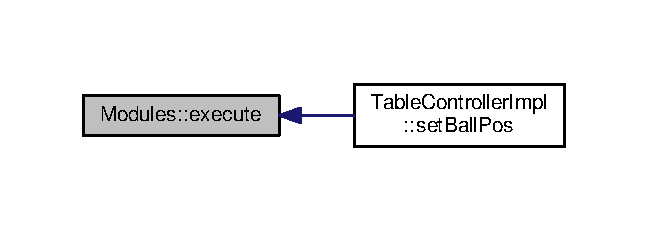
\includegraphics[width=311pt]{class_modules_a37a7813533ef4fdce805609ace458207_icgraph}
\end{center}
\end{figure}


\index{Modules@{Modules}!instance@{instance}}
\index{instance@{instance}!Modules@{Modules}}
\subsubsection[{\texorpdfstring{instance()}{instance()}}]{\setlength{\rightskip}{0pt plus 5cm}static {\bf Modules}$\ast$ Modules\+::instance (
\begin{DoxyParamCaption}
{}
\end{DoxyParamCaption}
)\hspace{0.3cm}{\ttfamily [inline]}, {\ttfamily [static]}}\hypertarget{class_modules_a89c623a11268379d1f8516434d775460}{}\label{class_modules_a89c623a11268379d1f8516434d775460}
instance function

\begin{DoxyReturn}{Returns}
\+\_\+instance; 
\end{DoxyReturn}


Here is the caller graph for this function\+:\nopagebreak
\begin{figure}[H]
\begin{center}
\leavevmode
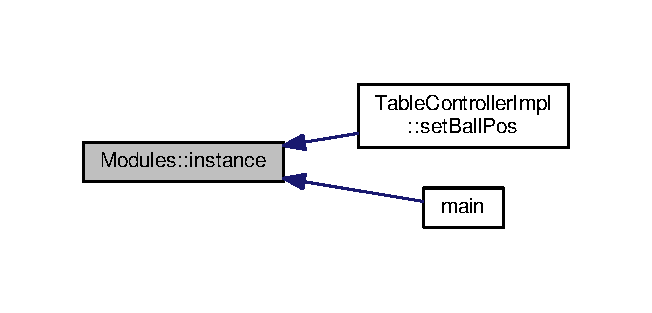
\includegraphics[width=313pt]{class_modules_a89c623a11268379d1f8516434d775460_icgraph}
\end{center}
\end{figure}


\index{Modules@{Modules}!register\+Function@{register\+Function}}
\index{register\+Function@{register\+Function}!Modules@{Modules}}
\subsubsection[{\texorpdfstring{register\+Function(const char $\ast$name, fp function)}{registerFunction(const char *name, fp function)}}]{\setlength{\rightskip}{0pt plus 5cm}void Modules\+::register\+Function (
\begin{DoxyParamCaption}
\item[{const char $\ast$}]{name, }
\item[{{\bf fp}}]{function}
\end{DoxyParamCaption}
)\hspace{0.3cm}{\ttfamily [inline]}}\hypertarget{class_modules_a01735870f0eb88e2847a822be229f927}{}\label{class_modules_a01735870f0eb88e2847a822be229f927}
register\+Function funktion

Throws \hyperlink{class_function_allready_registered_exception}{Function\+Allready\+Registered\+Exception} if the function has been registered before.


\begin{DoxyParams}{Parameters}
{\em (const} & char$\ast$ name, fp function) \\
\hline
\end{DoxyParams}


Here is the caller graph for this function\+:\nopagebreak
\begin{figure}[H]
\begin{center}
\leavevmode
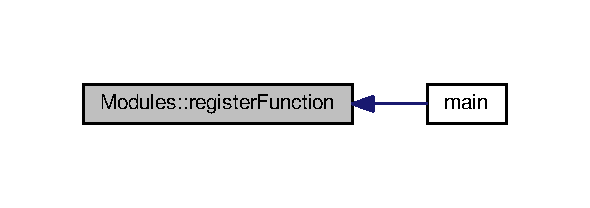
\includegraphics[width=283pt]{class_modules_a01735870f0eb88e2847a822be229f927_icgraph}
\end{center}
\end{figure}




\subsection{Member Data Documentation}
\index{Modules@{Modules}!\+\_\+instance@{\+\_\+instance}}
\index{\+\_\+instance@{\+\_\+instance}!Modules@{Modules}}
\subsubsection[{\texorpdfstring{\+\_\+instance}{_instance}}]{\setlength{\rightskip}{0pt plus 5cm}{\bf Modules} $\ast$ Modules\+::\+\_\+instance = 0\hspace{0.3cm}{\ttfamily [static]}, {\ttfamily [protected]}}\hypertarget{class_modules_ad82835853c834bfec3aa53da4b75def4}{}\label{class_modules_ad82835853c834bfec3aa53da4b75def4}
\index{Modules@{Modules}!cr@{cr}}
\index{cr@{cr}!Modules@{Modules}}
\subsubsection[{\texorpdfstring{cr}{cr}}]{\setlength{\rightskip}{0pt plus 5cm}{\bf Config\+Reader} Modules\+::cr\hspace{0.3cm}{\ttfamily [protected]}}\hypertarget{class_modules_a26598b42bad97f63a6662078afb61af4}{}\label{class_modules_a26598b42bad97f63a6662078afb61af4}
\index{Modules@{Modules}!functions@{functions}}
\index{functions@{functions}!Modules@{Modules}}
\subsubsection[{\texorpdfstring{functions}{functions}}]{\setlength{\rightskip}{0pt plus 5cm}std\+::map$<$std\+::string, {\bf fp}$>$ Modules\+::functions\hspace{0.3cm}{\ttfamily [protected]}}\hypertarget{class_modules_a96b175e7cd625d536d12f9c5e4aa8318}{}\label{class_modules_a96b175e7cd625d536d12f9c5e4aa8318}


The documentation for this class was generated from the following files\+:\begin{DoxyCompactItemize}
\item 
Kick\+I\+T@\+Eclipse/4\+\_\+\+Utilities/\hyperlink{_modules_8hpp}{Modules.\+hpp}\item 
Kick\+I\+T@\+Eclipse/\hyperlink{_kick_i_t_0D_eclipse_8cpp}{Kick\+I\+T@\+Eclipse.\+cpp}\end{DoxyCompactItemize}

\hypertarget{class_motor_communicator_interface}{}\section{Motor\+Communicator\+Interface Class Reference}
\label{class_motor_communicator_interface}\index{Motor\+Communicator\+Interface@{Motor\+Communicator\+Interface}}


{\ttfamily \#include $<$\+\_\+\+Motor\+Communicator\+Interface.\+hpp$>$}



Inheritance diagram for Motor\+Communicator\+Interface\+:\nopagebreak
\begin{figure}[H]
\begin{center}
\leavevmode
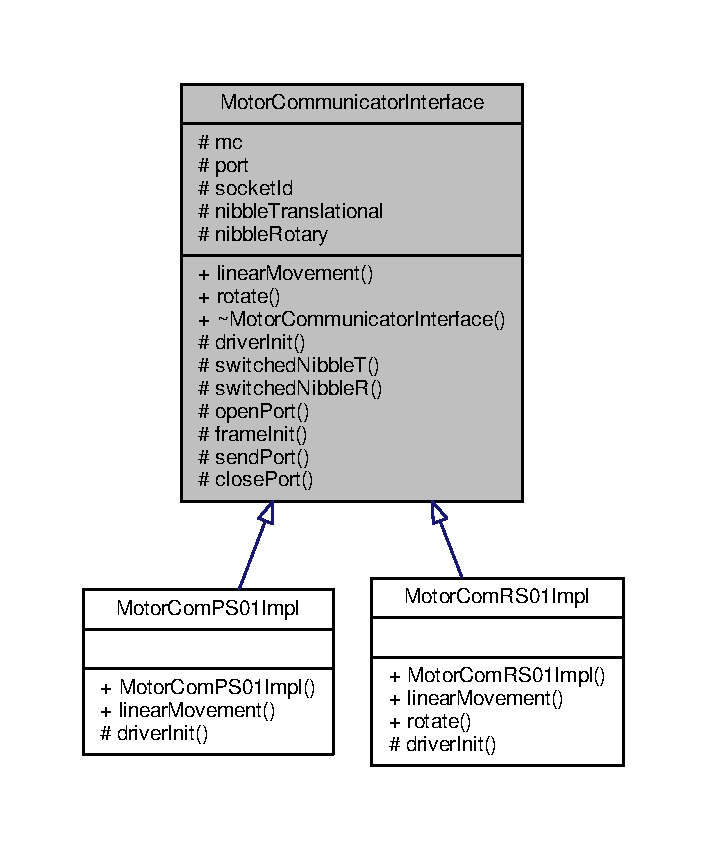
\includegraphics[width=340pt]{class_motor_communicator_interface__inherit__graph}
\end{center}
\end{figure}


Collaboration diagram for Motor\+Communicator\+Interface\+:\nopagebreak
\begin{figure}[H]
\begin{center}
\leavevmode
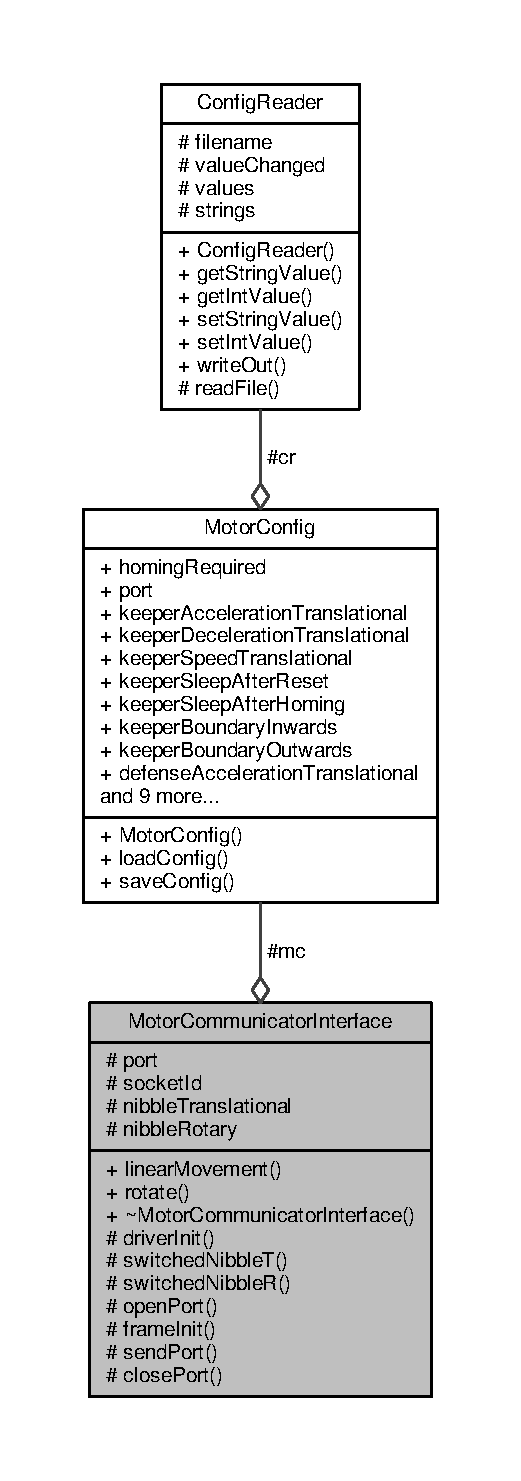
\includegraphics[height=550pt]{class_motor_communicator_interface__coll__graph}
\end{center}
\end{figure}
\subsection*{Public Member Functions}
\begin{DoxyCompactItemize}
\item 
virtual void \hyperlink{class_motor_communicator_interface_ac4621f673547a5c0b63207348cef69d3}{linear\+Movement} (int position)=0
\item 
virtual void \hyperlink{class_motor_communicator_interface_a9b80ed5df32b6a079326b71832353c41}{rotate} (int amount)
\item 
virtual \hyperlink{class_motor_communicator_interface_a12d122da47f6ba863e7a8f7c838155b8}{$\sim$\+Motor\+Communicator\+Interface} ()
\end{DoxyCompactItemize}
\subsection*{Protected Member Functions}
\begin{DoxyCompactItemize}
\item 
virtual void \hyperlink{class_motor_communicator_interface_a8ba57825f67ba4e1230c73fec5882ec5}{driver\+Init} ()=0
\item 
int \hyperlink{class_motor_communicator_interface_ab86c8e346dc6efb006b62d3329559ae6}{switched\+NibbleT} ()
\item 
int \hyperlink{class_motor_communicator_interface_afe256f56dfb26e7abe1f2eb102e1129c}{switched\+NibbleR} ()
\item 
int \hyperlink{class_motor_communicator_interface_a9b611145c47f1d8842eb9411d9e0e95a}{open\+Port} ()
\item 
void \hyperlink{class_motor_communicator_interface_a833096f7dfe3a034f30f53fb6f380f3b}{frame\+Init} (int ID, int D\+LC, int Data\+\_\+0, int Data\+\_\+1, int Data\+\_\+2, int Data\+\_\+3, int Data\+\_\+4, int Data\+\_\+5, int Data\+\_\+6, int Data\+\_\+7)
\item 
int \hyperlink{class_motor_communicator_interface_a62511203d5a487dc7148c8f083d89d12}{send\+Port} (struct can\+\_\+frame $\ast$frame)
\item 
void \hyperlink{class_motor_communicator_interface_aa761210caa851871c73732955e1eadba}{close\+Port} ()
\end{DoxyCompactItemize}
\subsection*{Protected Attributes}
\begin{DoxyCompactItemize}
\item 
\hyperlink{class_motor_config}{Motor\+Config} \hyperlink{class_motor_communicator_interface_aae1e504fe7cce7e933b77d8e31a96878}{mc}
\item 
char $\ast$ \hyperlink{class_motor_communicator_interface_adde2a840f8e9cd2e43b34af2bf8c3719}{port}
\item 
int \hyperlink{class_motor_communicator_interface_ad4d2f463fa6182b86bee4852dcee3d3a}{socket\+Id}
\item 
char \hyperlink{class_motor_communicator_interface_ae3010f217b379f0f62ebd5fee8387f21}{nibble\+Translational} = 1
\item 
char \hyperlink{class_motor_communicator_interface_af57ae9b19b30f4e7fc07545629117ad9}{nibble\+Rotary} = 1
\end{DoxyCompactItemize}


\subsection{Detailed Description}
\hyperlink{class_motor_communicator_interface}{Motor\+Communicator\+Interface} class 

\subsection{Constructor \& Destructor Documentation}
\index{Motor\+Communicator\+Interface@{Motor\+Communicator\+Interface}!````~Motor\+Communicator\+Interface@{$\sim$\+Motor\+Communicator\+Interface}}
\index{````~Motor\+Communicator\+Interface@{$\sim$\+Motor\+Communicator\+Interface}!Motor\+Communicator\+Interface@{Motor\+Communicator\+Interface}}
\subsubsection[{\texorpdfstring{$\sim$\+Motor\+Communicator\+Interface()}{~MotorCommunicatorInterface()}}]{\setlength{\rightskip}{0pt plus 5cm}virtual Motor\+Communicator\+Interface\+::$\sim$\+Motor\+Communicator\+Interface (
\begin{DoxyParamCaption}
{}
\end{DoxyParamCaption}
)\hspace{0.3cm}{\ttfamily [inline]}, {\ttfamily [virtual]}}\hypertarget{class_motor_communicator_interface_a12d122da47f6ba863e7a8f7c838155b8}{}\label{class_motor_communicator_interface_a12d122da47f6ba863e7a8f7c838155b8}
\hyperlink{class_motor_communicator_interface}{Motor\+Communicator\+Interface} destructor 

\subsection{Member Function Documentation}
\index{Motor\+Communicator\+Interface@{Motor\+Communicator\+Interface}!close\+Port@{close\+Port}}
\index{close\+Port@{close\+Port}!Motor\+Communicator\+Interface@{Motor\+Communicator\+Interface}}
\subsubsection[{\texorpdfstring{close\+Port()}{closePort()}}]{\setlength{\rightskip}{0pt plus 5cm}void Motor\+Communicator\+Interface\+::close\+Port (
\begin{DoxyParamCaption}
{}
\end{DoxyParamCaption}
)\hspace{0.3cm}{\ttfamily [inline]}, {\ttfamily [protected]}}\hypertarget{class_motor_communicator_interface_aa761210caa851871c73732955e1eadba}{}\label{class_motor_communicator_interface_aa761210caa851871c73732955e1eadba}
close\+Port funktion 

Here is the caller graph for this function\+:\nopagebreak
\begin{figure}[H]
\begin{center}
\leavevmode
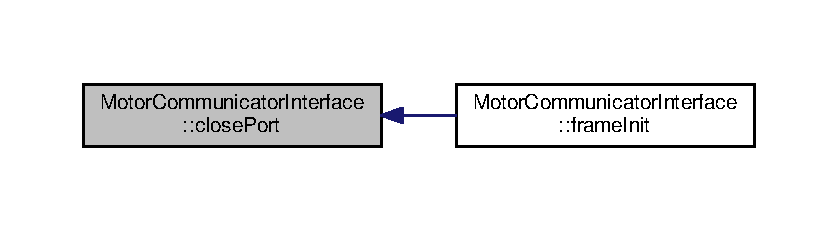
\includegraphics[width=350pt]{class_motor_communicator_interface_aa761210caa851871c73732955e1eadba_icgraph}
\end{center}
\end{figure}


\index{Motor\+Communicator\+Interface@{Motor\+Communicator\+Interface}!driver\+Init@{driver\+Init}}
\index{driver\+Init@{driver\+Init}!Motor\+Communicator\+Interface@{Motor\+Communicator\+Interface}}
\subsubsection[{\texorpdfstring{driver\+Init()=0}{driverInit()=0}}]{\setlength{\rightskip}{0pt plus 5cm}virtual void Motor\+Communicator\+Interface\+::driver\+Init (
\begin{DoxyParamCaption}
{}
\end{DoxyParamCaption}
)\hspace{0.3cm}{\ttfamily [protected]}, {\ttfamily [pure virtual]}}\hypertarget{class_motor_communicator_interface_a8ba57825f67ba4e1230c73fec5882ec5}{}\label{class_motor_communicator_interface_a8ba57825f67ba4e1230c73fec5882ec5}
driver\+Init function 

Implemented in \hyperlink{class_motor_com_r_s01_impl_a958cf9b3e05aba957af3e6df80e4ec2f}{Motor\+Com\+R\+S01\+Impl}, and \hyperlink{class_motor_com_p_s01_impl_a323cd48a50c38949c3349924262395c0}{Motor\+Com\+P\+S01\+Impl}.

\index{Motor\+Communicator\+Interface@{Motor\+Communicator\+Interface}!frame\+Init@{frame\+Init}}
\index{frame\+Init@{frame\+Init}!Motor\+Communicator\+Interface@{Motor\+Communicator\+Interface}}
\subsubsection[{\texorpdfstring{frame\+Init(int I\+D, int D\+L\+C, int Data\+\_\+0, int Data\+\_\+1, int Data\+\_\+2, int Data\+\_\+3, int Data\+\_\+4, int Data\+\_\+5, int Data\+\_\+6, int Data\+\_\+7)}{frameInit(int ID, int DLC, int Data_0, int Data_1, int Data_2, int Data_3, int Data_4, int Data_5, int Data_6, int Data_7)}}]{\setlength{\rightskip}{0pt plus 5cm}void Motor\+Communicator\+Interface\+::frame\+Init (
\begin{DoxyParamCaption}
\item[{int}]{ID, }
\item[{int}]{D\+LC, }
\item[{int}]{Data\+\_\+0, }
\item[{int}]{Data\+\_\+1, }
\item[{int}]{Data\+\_\+2, }
\item[{int}]{Data\+\_\+3, }
\item[{int}]{Data\+\_\+4, }
\item[{int}]{Data\+\_\+5, }
\item[{int}]{Data\+\_\+6, }
\item[{int}]{Data\+\_\+7}
\end{DoxyParamCaption}
)\hspace{0.3cm}{\ttfamily [inline]}, {\ttfamily [protected]}}\hypertarget{class_motor_communicator_interface_a833096f7dfe3a034f30f53fb6f380f3b}{}\label{class_motor_communicator_interface_a833096f7dfe3a034f30f53fb6f380f3b}
frame\+Init function 
\begin{DoxyParams}{Parameters}
{\em } & \\
\hline
\end{DoxyParams}


Here is the call graph for this function\+:\nopagebreak
\begin{figure}[H]
\begin{center}
\leavevmode
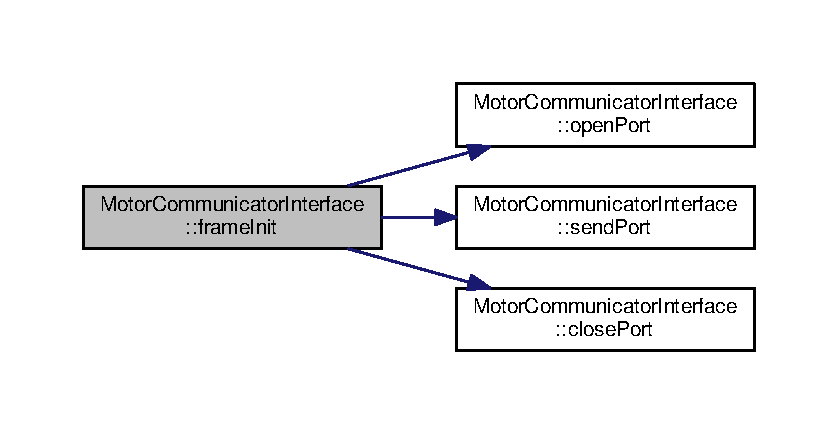
\includegraphics[width=350pt]{class_motor_communicator_interface_a833096f7dfe3a034f30f53fb6f380f3b_cgraph}
\end{center}
\end{figure}


\index{Motor\+Communicator\+Interface@{Motor\+Communicator\+Interface}!linear\+Movement@{linear\+Movement}}
\index{linear\+Movement@{linear\+Movement}!Motor\+Communicator\+Interface@{Motor\+Communicator\+Interface}}
\subsubsection[{\texorpdfstring{linear\+Movement(int position)=0}{linearMovement(int position)=0}}]{\setlength{\rightskip}{0pt plus 5cm}virtual void Motor\+Communicator\+Interface\+::linear\+Movement (
\begin{DoxyParamCaption}
\item[{int}]{position}
\end{DoxyParamCaption}
)\hspace{0.3cm}{\ttfamily [pure virtual]}}\hypertarget{class_motor_communicator_interface_ac4621f673547a5c0b63207348cef69d3}{}\label{class_motor_communicator_interface_ac4621f673547a5c0b63207348cef69d3}
linear\+Movement finction 
\begin{DoxyParams}{Parameters}
{\em int} & position \\
\hline
\end{DoxyParams}


Implemented in \hyperlink{class_motor_com_p_s01_impl_ae47ca67174e3240e18e129b5193a1ddc}{Motor\+Com\+P\+S01\+Impl}, and \hyperlink{class_motor_com_r_s01_impl_a329b9e6783f49d16ad6a57a34b1d29a3}{Motor\+Com\+R\+S01\+Impl}.



Here is the caller graph for this function\+:\nopagebreak
\begin{figure}[H]
\begin{center}
\leavevmode
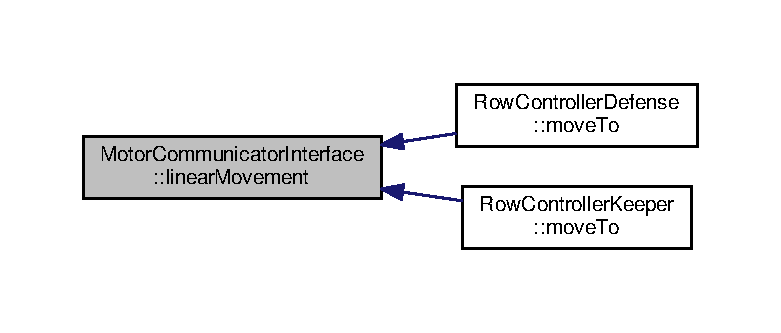
\includegraphics[width=350pt]{class_motor_communicator_interface_ac4621f673547a5c0b63207348cef69d3_icgraph}
\end{center}
\end{figure}


\index{Motor\+Communicator\+Interface@{Motor\+Communicator\+Interface}!open\+Port@{open\+Port}}
\index{open\+Port@{open\+Port}!Motor\+Communicator\+Interface@{Motor\+Communicator\+Interface}}
\subsubsection[{\texorpdfstring{open\+Port()}{openPort()}}]{\setlength{\rightskip}{0pt plus 5cm}int Motor\+Communicator\+Interface\+::open\+Port (
\begin{DoxyParamCaption}
{}
\end{DoxyParamCaption}
)\hspace{0.3cm}{\ttfamily [inline]}, {\ttfamily [protected]}}\hypertarget{class_motor_communicator_interface_a9b611145c47f1d8842eb9411d9e0e95a}{}\label{class_motor_communicator_interface_a9b611145c47f1d8842eb9411d9e0e95a}
open\+Port function \begin{DoxyReturn}{Returns}
0 or return -\/1 
\end{DoxyReturn}


Here is the caller graph for this function\+:\nopagebreak
\begin{figure}[H]
\begin{center}
\leavevmode
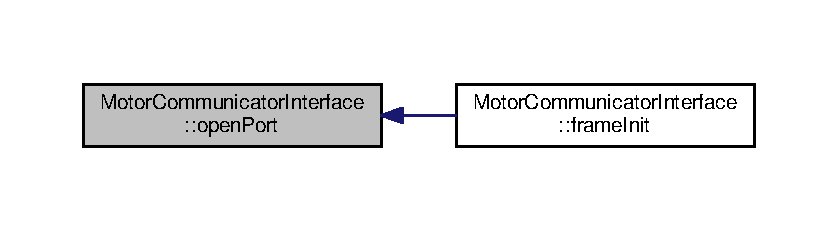
\includegraphics[width=350pt]{class_motor_communicator_interface_a9b611145c47f1d8842eb9411d9e0e95a_icgraph}
\end{center}
\end{figure}


\index{Motor\+Communicator\+Interface@{Motor\+Communicator\+Interface}!rotate@{rotate}}
\index{rotate@{rotate}!Motor\+Communicator\+Interface@{Motor\+Communicator\+Interface}}
\subsubsection[{\texorpdfstring{rotate(int amount)}{rotate(int amount)}}]{\setlength{\rightskip}{0pt plus 5cm}virtual void Motor\+Communicator\+Interface\+::rotate (
\begin{DoxyParamCaption}
\item[{int}]{amount}
\end{DoxyParamCaption}
)\hspace{0.3cm}{\ttfamily [inline]}, {\ttfamily [virtual]}}\hypertarget{class_motor_communicator_interface_a9b80ed5df32b6a079326b71832353c41}{}\label{class_motor_communicator_interface_a9b80ed5df32b6a079326b71832353c41}
rotate function 
\begin{DoxyParams}{Parameters}
{\em int} & amount \\
\hline
\end{DoxyParams}


Reimplemented in \hyperlink{class_motor_com_r_s01_impl_aacd356794c8c05da436e52293b41476d}{Motor\+Com\+R\+S01\+Impl}.



Here is the caller graph for this function\+:\nopagebreak
\begin{figure}[H]
\begin{center}
\leavevmode
\includegraphics[width=350pt]{class_motor_communicator_interface_a9b80ed5df32b6a079326b71832353c41_icgraph}
\end{center}
\end{figure}


\index{Motor\+Communicator\+Interface@{Motor\+Communicator\+Interface}!send\+Port@{send\+Port}}
\index{send\+Port@{send\+Port}!Motor\+Communicator\+Interface@{Motor\+Communicator\+Interface}}
\subsubsection[{\texorpdfstring{send\+Port(struct can\+\_\+frame $\ast$frame)}{sendPort(struct can_frame *frame)}}]{\setlength{\rightskip}{0pt plus 5cm}int Motor\+Communicator\+Interface\+::send\+Port (
\begin{DoxyParamCaption}
\item[{struct can\+\_\+frame $\ast$}]{frame}
\end{DoxyParamCaption}
)\hspace{0.3cm}{\ttfamily [inline]}, {\ttfamily [protected]}}\hypertarget{class_motor_communicator_interface_a62511203d5a487dc7148c8f083d89d12}{}\label{class_motor_communicator_interface_a62511203d5a487dc7148c8f083d89d12}
send\+Port function 
\begin{DoxyParams}{Parameters}
{\em struct} & can\+\_\+frame $\ast$frame \\
\hline
\end{DoxyParams}
\begin{DoxyReturn}{Returns}
0 or return -\/1 
\end{DoxyReturn}


Here is the caller graph for this function\+:\nopagebreak
\begin{figure}[H]
\begin{center}
\leavevmode
\includegraphics[width=350pt]{class_motor_communicator_interface_a62511203d5a487dc7148c8f083d89d12_icgraph}
\end{center}
\end{figure}


\index{Motor\+Communicator\+Interface@{Motor\+Communicator\+Interface}!switched\+NibbleR@{switched\+NibbleR}}
\index{switched\+NibbleR@{switched\+NibbleR}!Motor\+Communicator\+Interface@{Motor\+Communicator\+Interface}}
\subsubsection[{\texorpdfstring{switched\+Nibble\+R()}{switchedNibbleR()}}]{\setlength{\rightskip}{0pt plus 5cm}int Motor\+Communicator\+Interface\+::switched\+NibbleR (
\begin{DoxyParamCaption}
{}
\end{DoxyParamCaption}
)\hspace{0.3cm}{\ttfamily [inline]}, {\ttfamily [protected]}}\hypertarget{class_motor_communicator_interface_afe256f56dfb26e7abe1f2eb102e1129c}{}\label{class_motor_communicator_interface_afe256f56dfb26e7abe1f2eb102e1129c}
switched\+NibbleR function \begin{DoxyReturn}{Returns}
nibble\+Rotary 
\end{DoxyReturn}
\index{Motor\+Communicator\+Interface@{Motor\+Communicator\+Interface}!switched\+NibbleT@{switched\+NibbleT}}
\index{switched\+NibbleT@{switched\+NibbleT}!Motor\+Communicator\+Interface@{Motor\+Communicator\+Interface}}
\subsubsection[{\texorpdfstring{switched\+Nibble\+T()}{switchedNibbleT()}}]{\setlength{\rightskip}{0pt plus 5cm}int Motor\+Communicator\+Interface\+::switched\+NibbleT (
\begin{DoxyParamCaption}
{}
\end{DoxyParamCaption}
)\hspace{0.3cm}{\ttfamily [inline]}, {\ttfamily [protected]}}\hypertarget{class_motor_communicator_interface_ab86c8e346dc6efb006b62d3329559ae6}{}\label{class_motor_communicator_interface_ab86c8e346dc6efb006b62d3329559ae6}
switched\+NibbleT function 

\subsection{Member Data Documentation}
\index{Motor\+Communicator\+Interface@{Motor\+Communicator\+Interface}!mc@{mc}}
\index{mc@{mc}!Motor\+Communicator\+Interface@{Motor\+Communicator\+Interface}}
\subsubsection[{\texorpdfstring{mc}{mc}}]{\setlength{\rightskip}{0pt plus 5cm}{\bf Motor\+Config} Motor\+Communicator\+Interface\+::mc\hspace{0.3cm}{\ttfamily [protected]}}\hypertarget{class_motor_communicator_interface_aae1e504fe7cce7e933b77d8e31a96878}{}\label{class_motor_communicator_interface_aae1e504fe7cce7e933b77d8e31a96878}
\index{Motor\+Communicator\+Interface@{Motor\+Communicator\+Interface}!nibble\+Rotary@{nibble\+Rotary}}
\index{nibble\+Rotary@{nibble\+Rotary}!Motor\+Communicator\+Interface@{Motor\+Communicator\+Interface}}
\subsubsection[{\texorpdfstring{nibble\+Rotary}{nibbleRotary}}]{\setlength{\rightskip}{0pt plus 5cm}char Motor\+Communicator\+Interface\+::nibble\+Rotary = 1\hspace{0.3cm}{\ttfamily [protected]}}\hypertarget{class_motor_communicator_interface_af57ae9b19b30f4e7fc07545629117ad9}{}\label{class_motor_communicator_interface_af57ae9b19b30f4e7fc07545629117ad9}
\index{Motor\+Communicator\+Interface@{Motor\+Communicator\+Interface}!nibble\+Translational@{nibble\+Translational}}
\index{nibble\+Translational@{nibble\+Translational}!Motor\+Communicator\+Interface@{Motor\+Communicator\+Interface}}
\subsubsection[{\texorpdfstring{nibble\+Translational}{nibbleTranslational}}]{\setlength{\rightskip}{0pt plus 5cm}char Motor\+Communicator\+Interface\+::nibble\+Translational = 1\hspace{0.3cm}{\ttfamily [protected]}}\hypertarget{class_motor_communicator_interface_ae3010f217b379f0f62ebd5fee8387f21}{}\label{class_motor_communicator_interface_ae3010f217b379f0f62ebd5fee8387f21}
\index{Motor\+Communicator\+Interface@{Motor\+Communicator\+Interface}!port@{port}}
\index{port@{port}!Motor\+Communicator\+Interface@{Motor\+Communicator\+Interface}}
\subsubsection[{\texorpdfstring{port}{port}}]{\setlength{\rightskip}{0pt plus 5cm}char$\ast$ Motor\+Communicator\+Interface\+::port\hspace{0.3cm}{\ttfamily [protected]}}\hypertarget{class_motor_communicator_interface_adde2a840f8e9cd2e43b34af2bf8c3719}{}\label{class_motor_communicator_interface_adde2a840f8e9cd2e43b34af2bf8c3719}
\index{Motor\+Communicator\+Interface@{Motor\+Communicator\+Interface}!socket\+Id@{socket\+Id}}
\index{socket\+Id@{socket\+Id}!Motor\+Communicator\+Interface@{Motor\+Communicator\+Interface}}
\subsubsection[{\texorpdfstring{socket\+Id}{socketId}}]{\setlength{\rightskip}{0pt plus 5cm}int Motor\+Communicator\+Interface\+::socket\+Id\hspace{0.3cm}{\ttfamily [protected]}}\hypertarget{class_motor_communicator_interface_ad4d2f463fa6182b86bee4852dcee3d3a}{}\label{class_motor_communicator_interface_ad4d2f463fa6182b86bee4852dcee3d3a}


The documentation for this class was generated from the following file\+:\begin{DoxyCompactItemize}
\item 
2\+\_\+\+Control/\+Motor\+Communication/\hyperlink{___motor_communicator_interface_8hpp}{\+\_\+\+Motor\+Communicator\+Interface.\+hpp}\end{DoxyCompactItemize}

\hypertarget{class_motor_com_p_s01_impl}{}\section{Motor\+Com\+P\+S01\+Impl Class Reference}
\label{class_motor_com_p_s01_impl}\index{Motor\+Com\+P\+S01\+Impl@{Motor\+Com\+P\+S01\+Impl}}


{\ttfamily \#include $<$Motor\+Com\+P\+S01\+Impl.\+hpp$>$}



Inheritance diagram for Motor\+Com\+P\+S01\+Impl\+:\nopagebreak
\begin{figure}[H]
\begin{center}
\leavevmode
\includegraphics[width=244pt]{class_motor_com_p_s01_impl__inherit__graph}
\end{center}
\end{figure}


Collaboration diagram for Motor\+Com\+P\+S01\+Impl\+:\nopagebreak
\begin{figure}[H]
\begin{center}
\leavevmode
\includegraphics[height=550pt]{class_motor_com_p_s01_impl__coll__graph}
\end{center}
\end{figure}
\subsection*{Public Member Functions}
\begin{DoxyCompactItemize}
\item 
\hyperlink{class_motor_com_p_s01_impl_a52dec4461022dee453eeb26ff1072420}{Motor\+Com\+P\+S01\+Impl} ()
\item 
void \hyperlink{class_motor_com_p_s01_impl_ae47ca67174e3240e18e129b5193a1ddc}{linear\+Movement} (int position)
\end{DoxyCompactItemize}
\subsection*{Protected Member Functions}
\begin{DoxyCompactItemize}
\item 
void \hyperlink{class_motor_com_p_s01_impl_a323cd48a50c38949c3349924262395c0}{driver\+Init} ()
\end{DoxyCompactItemize}
\subsection*{Additional Inherited Members}


\subsection{Detailed Description}
\hyperlink{class_motor_com_p_s01_impl}{Motor\+Com\+P\+S01\+Impl} class 

\subsection{Constructor \& Destructor Documentation}
\index{Motor\+Com\+P\+S01\+Impl@{Motor\+Com\+P\+S01\+Impl}!Motor\+Com\+P\+S01\+Impl@{Motor\+Com\+P\+S01\+Impl}}
\index{Motor\+Com\+P\+S01\+Impl@{Motor\+Com\+P\+S01\+Impl}!Motor\+Com\+P\+S01\+Impl@{Motor\+Com\+P\+S01\+Impl}}
\subsubsection[{\texorpdfstring{Motor\+Com\+P\+S01\+Impl()}{MotorComPS01Impl()}}]{\setlength{\rightskip}{0pt plus 5cm}Motor\+Com\+P\+S01\+Impl\+::\+Motor\+Com\+P\+S01\+Impl (
\begin{DoxyParamCaption}
{}
\end{DoxyParamCaption}
)}\hypertarget{class_motor_com_p_s01_impl_a52dec4461022dee453eeb26ff1072420}{}\label{class_motor_com_p_s01_impl_a52dec4461022dee453eeb26ff1072420}
\hyperlink{class_motor_com_p_s01_impl}{Motor\+Com\+P\+S01\+Impl} constructor 

Here is the call graph for this function\+:\nopagebreak
\begin{figure}[H]
\begin{center}
\leavevmode
\includegraphics[width=350pt]{class_motor_com_p_s01_impl_a52dec4461022dee453eeb26ff1072420_cgraph}
\end{center}
\end{figure}




\subsection{Member Function Documentation}
\index{Motor\+Com\+P\+S01\+Impl@{Motor\+Com\+P\+S01\+Impl}!driver\+Init@{driver\+Init}}
\index{driver\+Init@{driver\+Init}!Motor\+Com\+P\+S01\+Impl@{Motor\+Com\+P\+S01\+Impl}}
\subsubsection[{\texorpdfstring{driver\+Init()}{driverInit()}}]{\setlength{\rightskip}{0pt plus 5cm}void Motor\+Com\+P\+S01\+Impl\+::driver\+Init (
\begin{DoxyParamCaption}
{}
\end{DoxyParamCaption}
)\hspace{0.3cm}{\ttfamily [protected]}, {\ttfamily [virtual]}}\hypertarget{class_motor_com_p_s01_impl_a323cd48a50c38949c3349924262395c0}{}\label{class_motor_com_p_s01_impl_a323cd48a50c38949c3349924262395c0}
driver\+Init function

Initial setup of motor-\/drivers. Needs to be called after the motors were detached from power supply or have entered error-\/state(red L\+ED) 

Implements \hyperlink{class_motor_communicator_interface_a8ba57825f67ba4e1230c73fec5882ec5}{Motor\+Communicator\+Interface}.



Here is the caller graph for this function\+:\nopagebreak
\begin{figure}[H]
\begin{center}
\leavevmode
\includegraphics[width=350pt]{class_motor_com_p_s01_impl_a323cd48a50c38949c3349924262395c0_icgraph}
\end{center}
\end{figure}


\index{Motor\+Com\+P\+S01\+Impl@{Motor\+Com\+P\+S01\+Impl}!linear\+Movement@{linear\+Movement}}
\index{linear\+Movement@{linear\+Movement}!Motor\+Com\+P\+S01\+Impl@{Motor\+Com\+P\+S01\+Impl}}
\subsubsection[{\texorpdfstring{linear\+Movement(int position)}{linearMovement(int position)}}]{\setlength{\rightskip}{0pt plus 5cm}void Motor\+Com\+P\+S01\+Impl\+::linear\+Movement (
\begin{DoxyParamCaption}
\item[{int}]{position}
\end{DoxyParamCaption}
)\hspace{0.3cm}{\ttfamily [virtual]}}\hypertarget{class_motor_com_p_s01_impl_ae47ca67174e3240e18e129b5193a1ddc}{}\label{class_motor_com_p_s01_impl_ae47ca67174e3240e18e129b5193a1ddc}
linear\+Movement function


\begin{DoxyParams}{Parameters}
{\em int} & position\\
\hline
\end{DoxyParams}
Control for translational movement. 

Implements \hyperlink{class_motor_communicator_interface_ac4621f673547a5c0b63207348cef69d3}{Motor\+Communicator\+Interface}.



The documentation for this class was generated from the following files\+:\begin{DoxyCompactItemize}
\item 
Kick\+I\+T@\+Eclipse/2\+\_\+\+Control/\+Motor\+Communication/\hyperlink{_motor_com_p_s01_impl_8hpp}{Motor\+Com\+P\+S01\+Impl.\+hpp}\item 
Kick\+I\+T@\+Eclipse/2\+\_\+\+Control/\+Motor\+Communication/\hyperlink{_motor_com_p_s01_impl_8cpp}{Motor\+Com\+P\+S01\+Impl.\+cpp}\end{DoxyCompactItemize}

\hypertarget{class_motor_com_r_s01_impl}{}\section{Motor\+Com\+R\+S01\+Impl Class Reference}
\label{class_motor_com_r_s01_impl}\index{Motor\+Com\+R\+S01\+Impl@{Motor\+Com\+R\+S01\+Impl}}


{\ttfamily \#include $<$Motor\+Com\+R\+S01\+Impl.\+hpp$>$}



Inheritance diagram for Motor\+Com\+R\+S01\+Impl\+:\nopagebreak
\begin{figure}[H]
\begin{center}
\leavevmode
\includegraphics[width=244pt]{class_motor_com_r_s01_impl__inherit__graph}
\end{center}
\end{figure}


Collaboration diagram for Motor\+Com\+R\+S01\+Impl\+:\nopagebreak
\begin{figure}[H]
\begin{center}
\leavevmode
\includegraphics[height=550pt]{class_motor_com_r_s01_impl__coll__graph}
\end{center}
\end{figure}
\subsection*{Public Member Functions}
\begin{DoxyCompactItemize}
\item 
\hyperlink{class_motor_com_r_s01_impl_a1f30f6ac77e75f0d69ea83db894a5ccf}{Motor\+Com\+R\+S01\+Impl} ()
\item 
void \hyperlink{class_motor_com_r_s01_impl_a329b9e6783f49d16ad6a57a34b1d29a3}{linear\+Movement} (int position)
\item 
void \hyperlink{class_motor_com_r_s01_impl_aacd356794c8c05da436e52293b41476d}{rotate} (int amount)
\end{DoxyCompactItemize}
\subsection*{Protected Member Functions}
\begin{DoxyCompactItemize}
\item 
void \hyperlink{class_motor_com_r_s01_impl_a958cf9b3e05aba957af3e6df80e4ec2f}{driver\+Init} ()
\end{DoxyCompactItemize}
\subsection*{Additional Inherited Members}


\subsection{Detailed Description}
\hyperlink{class_motor_com_r_s01_impl}{Motor\+Com\+R\+S01\+Impl} class 

\subsection{Constructor \& Destructor Documentation}
\index{Motor\+Com\+R\+S01\+Impl@{Motor\+Com\+R\+S01\+Impl}!Motor\+Com\+R\+S01\+Impl@{Motor\+Com\+R\+S01\+Impl}}
\index{Motor\+Com\+R\+S01\+Impl@{Motor\+Com\+R\+S01\+Impl}!Motor\+Com\+R\+S01\+Impl@{Motor\+Com\+R\+S01\+Impl}}
\subsubsection[{\texorpdfstring{Motor\+Com\+R\+S01\+Impl()}{MotorComRS01Impl()}}]{\setlength{\rightskip}{0pt plus 5cm}Motor\+Com\+R\+S01\+Impl\+::\+Motor\+Com\+R\+S01\+Impl (
\begin{DoxyParamCaption}
{}
\end{DoxyParamCaption}
)}\hypertarget{class_motor_com_r_s01_impl_a1f30f6ac77e75f0d69ea83db894a5ccf}{}\label{class_motor_com_r_s01_impl_a1f30f6ac77e75f0d69ea83db894a5ccf}
\hyperlink{class_motor_com_r_s01_impl}{Motor\+Com\+R\+S01\+Impl} constructor 
\begin{DoxyParams}{Parameters}
{\em Row} & r \\
\hline
\end{DoxyParams}


Here is the call graph for this function\+:\nopagebreak
\begin{figure}[H]
\begin{center}
\leavevmode
\includegraphics[width=350pt]{class_motor_com_r_s01_impl_a1f30f6ac77e75f0d69ea83db894a5ccf_cgraph}
\end{center}
\end{figure}




\subsection{Member Function Documentation}
\index{Motor\+Com\+R\+S01\+Impl@{Motor\+Com\+R\+S01\+Impl}!driver\+Init@{driver\+Init}}
\index{driver\+Init@{driver\+Init}!Motor\+Com\+R\+S01\+Impl@{Motor\+Com\+R\+S01\+Impl}}
\subsubsection[{\texorpdfstring{driver\+Init()}{driverInit()}}]{\setlength{\rightskip}{0pt plus 5cm}void Motor\+Com\+R\+S01\+Impl\+::driver\+Init (
\begin{DoxyParamCaption}
{}
\end{DoxyParamCaption}
)\hspace{0.3cm}{\ttfamily [protected]}, {\ttfamily [virtual]}}\hypertarget{class_motor_com_r_s01_impl_a958cf9b3e05aba957af3e6df80e4ec2f}{}\label{class_motor_com_r_s01_impl_a958cf9b3e05aba957af3e6df80e4ec2f}
driver\+Init function 

Implements \hyperlink{class_motor_communicator_interface_a8ba57825f67ba4e1230c73fec5882ec5}{Motor\+Communicator\+Interface}.



Here is the caller graph for this function\+:\nopagebreak
\begin{figure}[H]
\begin{center}
\leavevmode
\includegraphics[width=350pt]{class_motor_com_r_s01_impl_a958cf9b3e05aba957af3e6df80e4ec2f_icgraph}
\end{center}
\end{figure}


\index{Motor\+Com\+R\+S01\+Impl@{Motor\+Com\+R\+S01\+Impl}!linear\+Movement@{linear\+Movement}}
\index{linear\+Movement@{linear\+Movement}!Motor\+Com\+R\+S01\+Impl@{Motor\+Com\+R\+S01\+Impl}}
\subsubsection[{\texorpdfstring{linear\+Movement(int position)}{linearMovement(int position)}}]{\setlength{\rightskip}{0pt plus 5cm}void Motor\+Com\+R\+S01\+Impl\+::linear\+Movement (
\begin{DoxyParamCaption}
\item[{int}]{position}
\end{DoxyParamCaption}
)\hspace{0.3cm}{\ttfamily [virtual]}}\hypertarget{class_motor_com_r_s01_impl_a329b9e6783f49d16ad6a57a34b1d29a3}{}\label{class_motor_com_r_s01_impl_a329b9e6783f49d16ad6a57a34b1d29a3}
linear\+Movement 
\begin{DoxyParams}{Parameters}
{\em int} & position \\
\hline
\end{DoxyParams}


Implements \hyperlink{class_motor_communicator_interface_ac4621f673547a5c0b63207348cef69d3}{Motor\+Communicator\+Interface}.

\index{Motor\+Com\+R\+S01\+Impl@{Motor\+Com\+R\+S01\+Impl}!rotate@{rotate}}
\index{rotate@{rotate}!Motor\+Com\+R\+S01\+Impl@{Motor\+Com\+R\+S01\+Impl}}
\subsubsection[{\texorpdfstring{rotate(int amount)}{rotate(int amount)}}]{\setlength{\rightskip}{0pt plus 5cm}void Motor\+Com\+R\+S01\+Impl\+::rotate (
\begin{DoxyParamCaption}
\item[{int}]{amount}
\end{DoxyParamCaption}
)\hspace{0.3cm}{\ttfamily [virtual]}}\hypertarget{class_motor_com_r_s01_impl_aacd356794c8c05da436e52293b41476d}{}\label{class_motor_com_r_s01_impl_aacd356794c8c05da436e52293b41476d}
rotate function 
\begin{DoxyParams}{Parameters}
{\em int} & amount \\
\hline
\end{DoxyParams}


Reimplemented from \hyperlink{class_motor_communicator_interface_a9b80ed5df32b6a079326b71832353c41}{Motor\+Communicator\+Interface}.



The documentation for this class was generated from the following files\+:\begin{DoxyCompactItemize}
\item 
2\+\_\+\+Control/\+Motor\+Communication/\hyperlink{_motor_com_r_s01_impl_8hpp}{Motor\+Com\+R\+S01\+Impl.\+hpp}\item 
2\+\_\+\+Control/\+Motor\+Communication/\hyperlink{_motor_com_r_s01_impl_8cpp}{Motor\+Com\+R\+S01\+Impl.\+cpp}\end{DoxyCompactItemize}

\hypertarget{class_motor_config}{}\section{Motor\+Config Class Reference}
\label{class_motor_config}\index{Motor\+Config@{Motor\+Config}}


{\ttfamily \#include $<$Motor\+Config.\+hpp$>$}



Collaboration diagram for Motor\+Config\+:\nopagebreak
\begin{figure}[H]
\begin{center}
\leavevmode
\includegraphics[width=250pt]{class_motor_config__coll__graph}
\end{center}
\end{figure}
\subsection*{Public Member Functions}
\begin{DoxyCompactItemize}
\item 
\hyperlink{class_motor_config_a466fa31fbd6ce247caa36d1ea94a5a66}{Motor\+Config} ()
\item 
void \hyperlink{class_motor_config_af31d365ad1485d9d06180d4e264d1fa8}{load\+Config} ()
\item 
void \hyperlink{class_motor_config_aa9d5ac8fd14a9e7ed1c4c73e0030b161}{save\+Config} ()
\end{DoxyCompactItemize}
\subsection*{Public Attributes}
\begin{DoxyCompactItemize}
\item 
int \hyperlink{class_motor_config_ad682f2456ab31ef096e109cecd035838}{homing\+Required}
\item 
std\+::string \hyperlink{class_motor_config_a8c20151468f9399aaa7311b421ea16da}{port}
\item 
int \hyperlink{class_motor_config_a1eb04b17920041b277c713e85d77654a}{keeper\+Acceleration\+Translational}
\item 
int \hyperlink{class_motor_config_a7150d8f715063d1f554a782386f3a2d4}{keeper\+Deceleration\+Translational}
\item 
int \hyperlink{class_motor_config_a2d71d5ba5fa077680a8e032654f3e963}{keeper\+Speed\+Translational}
\item 
int \hyperlink{class_motor_config_a997c83a3797a6c7b7f6727bbf5bb14bf}{keeper\+Sleep\+After\+Reset}
\item 
int \hyperlink{class_motor_config_acbd8a628842a29b8d2e00913ab12804d}{keeper\+Sleep\+After\+Homing}
\item 
int \hyperlink{class_motor_config_a6fd5140bdaded8a7f8f0e92b2b6a47ba}{keeper\+Boundary\+Inwards}
\item 
int \hyperlink{class_motor_config_aff93b4ab4ba55fdb1798d98e1f0cfa84}{keeper\+Boundary\+Outwards}
\item 
int \hyperlink{class_motor_config_a313a2d1c68cff0a019df7ae26b108ab5}{defense\+Acceleration\+Translational}
\item 
int \hyperlink{class_motor_config_ae45b9d75d61b3299cd705c038ddf1ebe}{defense\+Acceleration\+Rotary}
\item 
int \hyperlink{class_motor_config_a592d9fc3b1b695652f5c429b74b43b4d}{defense\+Deceleration\+Translational}
\item 
int \hyperlink{class_motor_config_a90e7d6b520e9f07addf6d190c3302a1e}{defense\+Deceleration\+Rotary}
\item 
int \hyperlink{class_motor_config_a83d498372b0f3c95ed7324c4046cbd6f}{defense\+Speed\+Translational}
\item 
int \hyperlink{class_motor_config_a23fe81b56ecce25f87aaaa8208569add}{defense\+Speed\+Rotary}
\item 
int \hyperlink{class_motor_config_a9d559c7bf6caa1b2fdc9453d36f29c59}{defense\+Sleep\+After\+Reset}
\item 
int \hyperlink{class_motor_config_a3d21777d7d29dad713a0fbf225a6e29c}{defense\+Sleep\+After\+Homing}
\item 
int \hyperlink{class_motor_config_ac5352190d05d1754cd0408240bd2c1cb}{defense\+Boundary\+Inwards}
\item 
int \hyperlink{class_motor_config_a13f55df0545d8bb3682dfae26235b5bd}{defense\+Boundary\+Outwards}
\end{DoxyCompactItemize}
\subsection*{Protected Attributes}
\begin{DoxyCompactItemize}
\item 
\hyperlink{class_config_reader}{Config\+Reader} \hyperlink{class_motor_config_ae9cc5f54d202911ae6e445be554b2d13}{cr}
\end{DoxyCompactItemize}


\subsection{Detailed Description}
\hyperlink{class_motor_config}{Motor\+Config} class 

\subsection{Constructor \& Destructor Documentation}
\index{Motor\+Config@{Motor\+Config}!Motor\+Config@{Motor\+Config}}
\index{Motor\+Config@{Motor\+Config}!Motor\+Config@{Motor\+Config}}
\subsubsection[{\texorpdfstring{Motor\+Config()}{MotorConfig()}}]{\setlength{\rightskip}{0pt plus 5cm}Motor\+Config\+::\+Motor\+Config (
\begin{DoxyParamCaption}
{}
\end{DoxyParamCaption}
)\hspace{0.3cm}{\ttfamily [inline]}}\hypertarget{class_motor_config_a466fa31fbd6ce247caa36d1ea94a5a66}{}\label{class_motor_config_a466fa31fbd6ce247caa36d1ea94a5a66}
\hyperlink{class_motor_config}{Motor\+Config} constructor 

Here is the call graph for this function\+:\nopagebreak
\begin{figure}[H]
\begin{center}
\leavevmode
\includegraphics[width=350pt]{class_motor_config_a466fa31fbd6ce247caa36d1ea94a5a66_cgraph}
\end{center}
\end{figure}




\subsection{Member Function Documentation}
\index{Motor\+Config@{Motor\+Config}!load\+Config@{load\+Config}}
\index{load\+Config@{load\+Config}!Motor\+Config@{Motor\+Config}}
\subsubsection[{\texorpdfstring{load\+Config()}{loadConfig()}}]{\setlength{\rightskip}{0pt plus 5cm}void Motor\+Config\+::load\+Config (
\begin{DoxyParamCaption}
{}
\end{DoxyParamCaption}
)\hspace{0.3cm}{\ttfamily [inline]}}\hypertarget{class_motor_config_af31d365ad1485d9d06180d4e264d1fa8}{}\label{class_motor_config_af31d365ad1485d9d06180d4e264d1fa8}
load\+Config function 

Here is the call graph for this function\+:\nopagebreak
\begin{figure}[H]
\begin{center}
\leavevmode
\includegraphics[width=350pt]{class_motor_config_af31d365ad1485d9d06180d4e264d1fa8_cgraph}
\end{center}
\end{figure}




Here is the caller graph for this function\+:\nopagebreak
\begin{figure}[H]
\begin{center}
\leavevmode
\includegraphics[width=350pt]{class_motor_config_af31d365ad1485d9d06180d4e264d1fa8_icgraph}
\end{center}
\end{figure}


\index{Motor\+Config@{Motor\+Config}!save\+Config@{save\+Config}}
\index{save\+Config@{save\+Config}!Motor\+Config@{Motor\+Config}}
\subsubsection[{\texorpdfstring{save\+Config()}{saveConfig()}}]{\setlength{\rightskip}{0pt plus 5cm}void Motor\+Config\+::save\+Config (
\begin{DoxyParamCaption}
{}
\end{DoxyParamCaption}
)\hspace{0.3cm}{\ttfamily [inline]}}\hypertarget{class_motor_config_aa9d5ac8fd14a9e7ed1c4c73e0030b161}{}\label{class_motor_config_aa9d5ac8fd14a9e7ed1c4c73e0030b161}
save\+Config function 

Here is the call graph for this function\+:\nopagebreak
\begin{figure}[H]
\begin{center}
\leavevmode
\includegraphics[width=350pt]{class_motor_config_aa9d5ac8fd14a9e7ed1c4c73e0030b161_cgraph}
\end{center}
\end{figure}




\subsection{Member Data Documentation}
\index{Motor\+Config@{Motor\+Config}!cr@{cr}}
\index{cr@{cr}!Motor\+Config@{Motor\+Config}}
\subsubsection[{\texorpdfstring{cr}{cr}}]{\setlength{\rightskip}{0pt plus 5cm}{\bf Config\+Reader} Motor\+Config\+::cr\hspace{0.3cm}{\ttfamily [protected]}}\hypertarget{class_motor_config_ae9cc5f54d202911ae6e445be554b2d13}{}\label{class_motor_config_ae9cc5f54d202911ae6e445be554b2d13}
\index{Motor\+Config@{Motor\+Config}!defense\+Acceleration\+Rotary@{defense\+Acceleration\+Rotary}}
\index{defense\+Acceleration\+Rotary@{defense\+Acceleration\+Rotary}!Motor\+Config@{Motor\+Config}}
\subsubsection[{\texorpdfstring{defense\+Acceleration\+Rotary}{defenseAccelerationRotary}}]{\setlength{\rightskip}{0pt plus 5cm}int Motor\+Config\+::defense\+Acceleration\+Rotary}\hypertarget{class_motor_config_ae45b9d75d61b3299cd705c038ddf1ebe}{}\label{class_motor_config_ae45b9d75d61b3299cd705c038ddf1ebe}
\index{Motor\+Config@{Motor\+Config}!defense\+Acceleration\+Translational@{defense\+Acceleration\+Translational}}
\index{defense\+Acceleration\+Translational@{defense\+Acceleration\+Translational}!Motor\+Config@{Motor\+Config}}
\subsubsection[{\texorpdfstring{defense\+Acceleration\+Translational}{defenseAccelerationTranslational}}]{\setlength{\rightskip}{0pt plus 5cm}int Motor\+Config\+::defense\+Acceleration\+Translational}\hypertarget{class_motor_config_a313a2d1c68cff0a019df7ae26b108ab5}{}\label{class_motor_config_a313a2d1c68cff0a019df7ae26b108ab5}
\index{Motor\+Config@{Motor\+Config}!defense\+Boundary\+Inwards@{defense\+Boundary\+Inwards}}
\index{defense\+Boundary\+Inwards@{defense\+Boundary\+Inwards}!Motor\+Config@{Motor\+Config}}
\subsubsection[{\texorpdfstring{defense\+Boundary\+Inwards}{defenseBoundaryInwards}}]{\setlength{\rightskip}{0pt plus 5cm}int Motor\+Config\+::defense\+Boundary\+Inwards}\hypertarget{class_motor_config_ac5352190d05d1754cd0408240bd2c1cb}{}\label{class_motor_config_ac5352190d05d1754cd0408240bd2c1cb}
\index{Motor\+Config@{Motor\+Config}!defense\+Boundary\+Outwards@{defense\+Boundary\+Outwards}}
\index{defense\+Boundary\+Outwards@{defense\+Boundary\+Outwards}!Motor\+Config@{Motor\+Config}}
\subsubsection[{\texorpdfstring{defense\+Boundary\+Outwards}{defenseBoundaryOutwards}}]{\setlength{\rightskip}{0pt plus 5cm}int Motor\+Config\+::defense\+Boundary\+Outwards}\hypertarget{class_motor_config_a13f55df0545d8bb3682dfae26235b5bd}{}\label{class_motor_config_a13f55df0545d8bb3682dfae26235b5bd}
\index{Motor\+Config@{Motor\+Config}!defense\+Deceleration\+Rotary@{defense\+Deceleration\+Rotary}}
\index{defense\+Deceleration\+Rotary@{defense\+Deceleration\+Rotary}!Motor\+Config@{Motor\+Config}}
\subsubsection[{\texorpdfstring{defense\+Deceleration\+Rotary}{defenseDecelerationRotary}}]{\setlength{\rightskip}{0pt plus 5cm}int Motor\+Config\+::defense\+Deceleration\+Rotary}\hypertarget{class_motor_config_a90e7d6b520e9f07addf6d190c3302a1e}{}\label{class_motor_config_a90e7d6b520e9f07addf6d190c3302a1e}
\index{Motor\+Config@{Motor\+Config}!defense\+Deceleration\+Translational@{defense\+Deceleration\+Translational}}
\index{defense\+Deceleration\+Translational@{defense\+Deceleration\+Translational}!Motor\+Config@{Motor\+Config}}
\subsubsection[{\texorpdfstring{defense\+Deceleration\+Translational}{defenseDecelerationTranslational}}]{\setlength{\rightskip}{0pt plus 5cm}int Motor\+Config\+::defense\+Deceleration\+Translational}\hypertarget{class_motor_config_a592d9fc3b1b695652f5c429b74b43b4d}{}\label{class_motor_config_a592d9fc3b1b695652f5c429b74b43b4d}
\index{Motor\+Config@{Motor\+Config}!defense\+Sleep\+After\+Homing@{defense\+Sleep\+After\+Homing}}
\index{defense\+Sleep\+After\+Homing@{defense\+Sleep\+After\+Homing}!Motor\+Config@{Motor\+Config}}
\subsubsection[{\texorpdfstring{defense\+Sleep\+After\+Homing}{defenseSleepAfterHoming}}]{\setlength{\rightskip}{0pt plus 5cm}int Motor\+Config\+::defense\+Sleep\+After\+Homing}\hypertarget{class_motor_config_a3d21777d7d29dad713a0fbf225a6e29c}{}\label{class_motor_config_a3d21777d7d29dad713a0fbf225a6e29c}
\index{Motor\+Config@{Motor\+Config}!defense\+Sleep\+After\+Reset@{defense\+Sleep\+After\+Reset}}
\index{defense\+Sleep\+After\+Reset@{defense\+Sleep\+After\+Reset}!Motor\+Config@{Motor\+Config}}
\subsubsection[{\texorpdfstring{defense\+Sleep\+After\+Reset}{defenseSleepAfterReset}}]{\setlength{\rightskip}{0pt plus 5cm}int Motor\+Config\+::defense\+Sleep\+After\+Reset}\hypertarget{class_motor_config_a9d559c7bf6caa1b2fdc9453d36f29c59}{}\label{class_motor_config_a9d559c7bf6caa1b2fdc9453d36f29c59}
\index{Motor\+Config@{Motor\+Config}!defense\+Speed\+Rotary@{defense\+Speed\+Rotary}}
\index{defense\+Speed\+Rotary@{defense\+Speed\+Rotary}!Motor\+Config@{Motor\+Config}}
\subsubsection[{\texorpdfstring{defense\+Speed\+Rotary}{defenseSpeedRotary}}]{\setlength{\rightskip}{0pt plus 5cm}int Motor\+Config\+::defense\+Speed\+Rotary}\hypertarget{class_motor_config_a23fe81b56ecce25f87aaaa8208569add}{}\label{class_motor_config_a23fe81b56ecce25f87aaaa8208569add}
\index{Motor\+Config@{Motor\+Config}!defense\+Speed\+Translational@{defense\+Speed\+Translational}}
\index{defense\+Speed\+Translational@{defense\+Speed\+Translational}!Motor\+Config@{Motor\+Config}}
\subsubsection[{\texorpdfstring{defense\+Speed\+Translational}{defenseSpeedTranslational}}]{\setlength{\rightskip}{0pt plus 5cm}int Motor\+Config\+::defense\+Speed\+Translational}\hypertarget{class_motor_config_a83d498372b0f3c95ed7324c4046cbd6f}{}\label{class_motor_config_a83d498372b0f3c95ed7324c4046cbd6f}
\index{Motor\+Config@{Motor\+Config}!homing\+Required@{homing\+Required}}
\index{homing\+Required@{homing\+Required}!Motor\+Config@{Motor\+Config}}
\subsubsection[{\texorpdfstring{homing\+Required}{homingRequired}}]{\setlength{\rightskip}{0pt plus 5cm}int Motor\+Config\+::homing\+Required}\hypertarget{class_motor_config_ad682f2456ab31ef096e109cecd035838}{}\label{class_motor_config_ad682f2456ab31ef096e109cecd035838}
\index{Motor\+Config@{Motor\+Config}!keeper\+Acceleration\+Translational@{keeper\+Acceleration\+Translational}}
\index{keeper\+Acceleration\+Translational@{keeper\+Acceleration\+Translational}!Motor\+Config@{Motor\+Config}}
\subsubsection[{\texorpdfstring{keeper\+Acceleration\+Translational}{keeperAccelerationTranslational}}]{\setlength{\rightskip}{0pt plus 5cm}int Motor\+Config\+::keeper\+Acceleration\+Translational}\hypertarget{class_motor_config_a1eb04b17920041b277c713e85d77654a}{}\label{class_motor_config_a1eb04b17920041b277c713e85d77654a}
\index{Motor\+Config@{Motor\+Config}!keeper\+Boundary\+Inwards@{keeper\+Boundary\+Inwards}}
\index{keeper\+Boundary\+Inwards@{keeper\+Boundary\+Inwards}!Motor\+Config@{Motor\+Config}}
\subsubsection[{\texorpdfstring{keeper\+Boundary\+Inwards}{keeperBoundaryInwards}}]{\setlength{\rightskip}{0pt plus 5cm}int Motor\+Config\+::keeper\+Boundary\+Inwards}\hypertarget{class_motor_config_a6fd5140bdaded8a7f8f0e92b2b6a47ba}{}\label{class_motor_config_a6fd5140bdaded8a7f8f0e92b2b6a47ba}
\index{Motor\+Config@{Motor\+Config}!keeper\+Boundary\+Outwards@{keeper\+Boundary\+Outwards}}
\index{keeper\+Boundary\+Outwards@{keeper\+Boundary\+Outwards}!Motor\+Config@{Motor\+Config}}
\subsubsection[{\texorpdfstring{keeper\+Boundary\+Outwards}{keeperBoundaryOutwards}}]{\setlength{\rightskip}{0pt plus 5cm}int Motor\+Config\+::keeper\+Boundary\+Outwards}\hypertarget{class_motor_config_aff93b4ab4ba55fdb1798d98e1f0cfa84}{}\label{class_motor_config_aff93b4ab4ba55fdb1798d98e1f0cfa84}
\index{Motor\+Config@{Motor\+Config}!keeper\+Deceleration\+Translational@{keeper\+Deceleration\+Translational}}
\index{keeper\+Deceleration\+Translational@{keeper\+Deceleration\+Translational}!Motor\+Config@{Motor\+Config}}
\subsubsection[{\texorpdfstring{keeper\+Deceleration\+Translational}{keeperDecelerationTranslational}}]{\setlength{\rightskip}{0pt plus 5cm}int Motor\+Config\+::keeper\+Deceleration\+Translational}\hypertarget{class_motor_config_a7150d8f715063d1f554a782386f3a2d4}{}\label{class_motor_config_a7150d8f715063d1f554a782386f3a2d4}
\index{Motor\+Config@{Motor\+Config}!keeper\+Sleep\+After\+Homing@{keeper\+Sleep\+After\+Homing}}
\index{keeper\+Sleep\+After\+Homing@{keeper\+Sleep\+After\+Homing}!Motor\+Config@{Motor\+Config}}
\subsubsection[{\texorpdfstring{keeper\+Sleep\+After\+Homing}{keeperSleepAfterHoming}}]{\setlength{\rightskip}{0pt plus 5cm}int Motor\+Config\+::keeper\+Sleep\+After\+Homing}\hypertarget{class_motor_config_acbd8a628842a29b8d2e00913ab12804d}{}\label{class_motor_config_acbd8a628842a29b8d2e00913ab12804d}
\index{Motor\+Config@{Motor\+Config}!keeper\+Sleep\+After\+Reset@{keeper\+Sleep\+After\+Reset}}
\index{keeper\+Sleep\+After\+Reset@{keeper\+Sleep\+After\+Reset}!Motor\+Config@{Motor\+Config}}
\subsubsection[{\texorpdfstring{keeper\+Sleep\+After\+Reset}{keeperSleepAfterReset}}]{\setlength{\rightskip}{0pt plus 5cm}int Motor\+Config\+::keeper\+Sleep\+After\+Reset}\hypertarget{class_motor_config_a997c83a3797a6c7b7f6727bbf5bb14bf}{}\label{class_motor_config_a997c83a3797a6c7b7f6727bbf5bb14bf}
\index{Motor\+Config@{Motor\+Config}!keeper\+Speed\+Translational@{keeper\+Speed\+Translational}}
\index{keeper\+Speed\+Translational@{keeper\+Speed\+Translational}!Motor\+Config@{Motor\+Config}}
\subsubsection[{\texorpdfstring{keeper\+Speed\+Translational}{keeperSpeedTranslational}}]{\setlength{\rightskip}{0pt plus 5cm}int Motor\+Config\+::keeper\+Speed\+Translational}\hypertarget{class_motor_config_a2d71d5ba5fa077680a8e032654f3e963}{}\label{class_motor_config_a2d71d5ba5fa077680a8e032654f3e963}
\index{Motor\+Config@{Motor\+Config}!port@{port}}
\index{port@{port}!Motor\+Config@{Motor\+Config}}
\subsubsection[{\texorpdfstring{port}{port}}]{\setlength{\rightskip}{0pt plus 5cm}std\+::string Motor\+Config\+::port}\hypertarget{class_motor_config_a8c20151468f9399aaa7311b421ea16da}{}\label{class_motor_config_a8c20151468f9399aaa7311b421ea16da}


The documentation for this class was generated from the following file\+:\begin{DoxyCompactItemize}
\item 
Kick\+I\+T@\+Eclipse/5\+\_\+\+Data\+Type/\hyperlink{_motor_config_8hpp}{Motor\+Config.\+hpp}\end{DoxyCompactItemize}

\hypertarget{class_parameter_not_found_exception}{}\section{Parameter\+Not\+Found\+Exception Class Reference}
\label{class_parameter_not_found_exception}\index{Parameter\+Not\+Found\+Exception@{Parameter\+Not\+Found\+Exception}}


{\ttfamily \#include $<$Config\+Reader.\+hpp$>$}



Inheritance diagram for Parameter\+Not\+Found\+Exception\+:\nopagebreak
\begin{figure}[H]
\begin{center}
\leavevmode
\includegraphics[width=243pt]{class_parameter_not_found_exception__inherit__graph}
\end{center}
\end{figure}


Collaboration diagram for Parameter\+Not\+Found\+Exception\+:\nopagebreak
\begin{figure}[H]
\begin{center}
\leavevmode
\includegraphics[width=243pt]{class_parameter_not_found_exception__coll__graph}
\end{center}
\end{figure}
\subsection*{Public Member Functions}
\begin{DoxyCompactItemize}
\item 
\hyperlink{class_parameter_not_found_exception_a3de44f39ea25ba23db25405472273853}{Parameter\+Not\+Found\+Exception} (const char $\ast$name)
\end{DoxyCompactItemize}
\subsection*{Protected Attributes}
\begin{DoxyCompactItemize}
\item 
std\+::string \hyperlink{class_parameter_not_found_exception_ad7c9297e67fc1021feec3c74a6dcdffa}{p}
\end{DoxyCompactItemize}


\subsection{Detailed Description}
\hyperlink{class_parameter_not_found_exception}{Parameter\+Not\+Found\+Exception} class 

\subsection{Constructor \& Destructor Documentation}
\index{Parameter\+Not\+Found\+Exception@{Parameter\+Not\+Found\+Exception}!Parameter\+Not\+Found\+Exception@{Parameter\+Not\+Found\+Exception}}
\index{Parameter\+Not\+Found\+Exception@{Parameter\+Not\+Found\+Exception}!Parameter\+Not\+Found\+Exception@{Parameter\+Not\+Found\+Exception}}
\subsubsection[{\texorpdfstring{Parameter\+Not\+Found\+Exception(const char $\ast$name)}{ParameterNotFoundException(const char *name)}}]{\setlength{\rightskip}{0pt plus 5cm}Parameter\+Not\+Found\+Exception\+::\+Parameter\+Not\+Found\+Exception (
\begin{DoxyParamCaption}
\item[{const char $\ast$}]{name}
\end{DoxyParamCaption}
)\hspace{0.3cm}{\ttfamily [inline]}}\hypertarget{class_parameter_not_found_exception_a3de44f39ea25ba23db25405472273853}{}\label{class_parameter_not_found_exception_a3de44f39ea25ba23db25405472273853}
\hyperlink{class_parameter_not_found_exception}{Parameter\+Not\+Found\+Exception} function 
\begin{DoxyParams}{Parameters}
{\em (const} & char$\ast$ name)\+:p(name) \\
\hline
\end{DoxyParams}


\subsection{Member Data Documentation}
\index{Parameter\+Not\+Found\+Exception@{Parameter\+Not\+Found\+Exception}!p@{p}}
\index{p@{p}!Parameter\+Not\+Found\+Exception@{Parameter\+Not\+Found\+Exception}}
\subsubsection[{\texorpdfstring{p}{p}}]{\setlength{\rightskip}{0pt plus 5cm}std\+::string Parameter\+Not\+Found\+Exception\+::p\hspace{0.3cm}{\ttfamily [protected]}}\hypertarget{class_parameter_not_found_exception_ad7c9297e67fc1021feec3c74a6dcdffa}{}\label{class_parameter_not_found_exception_ad7c9297e67fc1021feec3c74a6dcdffa}


The documentation for this class was generated from the following file\+:\begin{DoxyCompactItemize}
\item 
4\+\_\+\+Utilities/\hyperlink{_config_reader_8hpp}{Config\+Reader.\+hpp}\end{DoxyCompactItemize}

\hypertarget{structqt__meta__stringdata___ball_tracker_impl__t}{}\section{qt\+\_\+meta\+\_\+stringdata\+\_\+\+Ball\+Tracker\+Impl\+\_\+t Struct Reference}
\label{structqt__meta__stringdata___ball_tracker_impl__t}\index{qt\+\_\+meta\+\_\+stringdata\+\_\+\+Ball\+Tracker\+Impl\+\_\+t@{qt\+\_\+meta\+\_\+stringdata\+\_\+\+Ball\+Tracker\+Impl\+\_\+t}}


Collaboration diagram for qt\+\_\+meta\+\_\+stringdata\+\_\+\+Ball\+Tracker\+Impl\+\_\+t\+:\nopagebreak
\begin{figure}[H]
\begin{center}
\leavevmode
\includegraphics[width=180pt]{structqt__meta__stringdata___ball_tracker_impl__t__coll__graph}
\end{center}
\end{figure}
\subsection*{Public Attributes}
\begin{DoxyCompactItemize}
\item 
Q\+Byte\+Array\+Data \hyperlink{structqt__meta__stringdata___ball_tracker_impl__t_aaa7d7ef4a4a293040f1ceb14790880db}{data} \mbox{[}3\mbox{]}
\item 
char \hyperlink{structqt__meta__stringdata___ball_tracker_impl__t_a04a60b2f79a2e3d26ef56213f357c24f}{stringdata0} \mbox{[}30\mbox{]}
\end{DoxyCompactItemize}


\subsection{Member Data Documentation}
\index{qt\+\_\+meta\+\_\+stringdata\+\_\+\+Ball\+Tracker\+Impl\+\_\+t@{qt\+\_\+meta\+\_\+stringdata\+\_\+\+Ball\+Tracker\+Impl\+\_\+t}!data@{data}}
\index{data@{data}!qt\+\_\+meta\+\_\+stringdata\+\_\+\+Ball\+Tracker\+Impl\+\_\+t@{qt\+\_\+meta\+\_\+stringdata\+\_\+\+Ball\+Tracker\+Impl\+\_\+t}}
\subsubsection[{\texorpdfstring{data}{data}}]{\setlength{\rightskip}{0pt plus 5cm}Q\+Byte\+Array\+Data qt\+\_\+meta\+\_\+stringdata\+\_\+\+Ball\+Tracker\+Impl\+\_\+t\+::data\mbox{[}3\mbox{]}}\hypertarget{structqt__meta__stringdata___ball_tracker_impl__t_aaa7d7ef4a4a293040f1ceb14790880db}{}\label{structqt__meta__stringdata___ball_tracker_impl__t_aaa7d7ef4a4a293040f1ceb14790880db}
\index{qt\+\_\+meta\+\_\+stringdata\+\_\+\+Ball\+Tracker\+Impl\+\_\+t@{qt\+\_\+meta\+\_\+stringdata\+\_\+\+Ball\+Tracker\+Impl\+\_\+t}!stringdata0@{stringdata0}}
\index{stringdata0@{stringdata0}!qt\+\_\+meta\+\_\+stringdata\+\_\+\+Ball\+Tracker\+Impl\+\_\+t@{qt\+\_\+meta\+\_\+stringdata\+\_\+\+Ball\+Tracker\+Impl\+\_\+t}}
\subsubsection[{\texorpdfstring{stringdata0}{stringdata0}}]{\setlength{\rightskip}{0pt plus 5cm}char qt\+\_\+meta\+\_\+stringdata\+\_\+\+Ball\+Tracker\+Impl\+\_\+t\+::stringdata0\mbox{[}30\mbox{]}}\hypertarget{structqt__meta__stringdata___ball_tracker_impl__t_a04a60b2f79a2e3d26ef56213f357c24f}{}\label{structqt__meta__stringdata___ball_tracker_impl__t_a04a60b2f79a2e3d26ef56213f357c24f}


The documentation for this struct was generated from the following file\+:\begin{DoxyCompactItemize}
\item 
build/\hyperlink{moc___ball_tracker_impl_8cpp}{moc\+\_\+\+Ball\+Tracker\+Impl.\+cpp}\end{DoxyCompactItemize}

\hypertarget{structqt__meta__stringdata___table_controller_impl__t}{}\section{qt\+\_\+meta\+\_\+stringdata\+\_\+\+Table\+Controller\+Impl\+\_\+t Struct Reference}
\label{structqt__meta__stringdata___table_controller_impl__t}\index{qt\+\_\+meta\+\_\+stringdata\+\_\+\+Table\+Controller\+Impl\+\_\+t@{qt\+\_\+meta\+\_\+stringdata\+\_\+\+Table\+Controller\+Impl\+\_\+t}}


Collaboration diagram for qt\+\_\+meta\+\_\+stringdata\+\_\+\+Table\+Controller\+Impl\+\_\+t\+:\nopagebreak
\begin{figure}[H]
\begin{center}
\leavevmode
\includegraphics[width=195pt]{structqt__meta__stringdata___table_controller_impl__t__coll__graph}
\end{center}
\end{figure}
\subsection*{Public Attributes}
\begin{DoxyCompactItemize}
\item 
Q\+Byte\+Array\+Data \hyperlink{structqt__meta__stringdata___table_controller_impl__t_abf949a0469f361c0c90653150fc8d0b3}{data} \mbox{[}5\mbox{]}
\item 
char \hyperlink{structqt__meta__stringdata___table_controller_impl__t_ad671611e780842223ffc0eb77564b446}{stringdata0} \mbox{[}49\mbox{]}
\end{DoxyCompactItemize}


\subsection{Member Data Documentation}
\index{qt\+\_\+meta\+\_\+stringdata\+\_\+\+Table\+Controller\+Impl\+\_\+t@{qt\+\_\+meta\+\_\+stringdata\+\_\+\+Table\+Controller\+Impl\+\_\+t}!data@{data}}
\index{data@{data}!qt\+\_\+meta\+\_\+stringdata\+\_\+\+Table\+Controller\+Impl\+\_\+t@{qt\+\_\+meta\+\_\+stringdata\+\_\+\+Table\+Controller\+Impl\+\_\+t}}
\subsubsection[{\texorpdfstring{data}{data}}]{\setlength{\rightskip}{0pt plus 5cm}Q\+Byte\+Array\+Data qt\+\_\+meta\+\_\+stringdata\+\_\+\+Table\+Controller\+Impl\+\_\+t\+::data\mbox{[}5\mbox{]}}\hypertarget{structqt__meta__stringdata___table_controller_impl__t_abf949a0469f361c0c90653150fc8d0b3}{}\label{structqt__meta__stringdata___table_controller_impl__t_abf949a0469f361c0c90653150fc8d0b3}
\index{qt\+\_\+meta\+\_\+stringdata\+\_\+\+Table\+Controller\+Impl\+\_\+t@{qt\+\_\+meta\+\_\+stringdata\+\_\+\+Table\+Controller\+Impl\+\_\+t}!stringdata0@{stringdata0}}
\index{stringdata0@{stringdata0}!qt\+\_\+meta\+\_\+stringdata\+\_\+\+Table\+Controller\+Impl\+\_\+t@{qt\+\_\+meta\+\_\+stringdata\+\_\+\+Table\+Controller\+Impl\+\_\+t}}
\subsubsection[{\texorpdfstring{stringdata0}{stringdata0}}]{\setlength{\rightskip}{0pt plus 5cm}char qt\+\_\+meta\+\_\+stringdata\+\_\+\+Table\+Controller\+Impl\+\_\+t\+::stringdata0\mbox{[}49\mbox{]}}\hypertarget{structqt__meta__stringdata___table_controller_impl__t_ad671611e780842223ffc0eb77564b446}{}\label{structqt__meta__stringdata___table_controller_impl__t_ad671611e780842223ffc0eb77564b446}


The documentation for this struct was generated from the following file\+:\begin{DoxyCompactItemize}
\item 
build/\hyperlink{moc___table_controller_impl_8cpp}{moc\+\_\+\+Table\+Controller\+Impl.\+cpp}\end{DoxyCompactItemize}

\hypertarget{class_row_controller_defense}{}\section{Row\+Controller\+Defense Class Reference}
\label{class_row_controller_defense}\index{Row\+Controller\+Defense@{Row\+Controller\+Defense}}


{\ttfamily \#include $<$Row\+Controller\+Defense.\+hpp$>$}



Inheritance diagram for Row\+Controller\+Defense\+:\nopagebreak
\begin{figure}[H]
\begin{center}
\leavevmode
\includegraphics[width=218pt]{class_row_controller_defense__inherit__graph}
\end{center}
\end{figure}


Collaboration diagram for Row\+Controller\+Defense\+:\nopagebreak
\begin{figure}[H]
\begin{center}
\leavevmode
\includegraphics[height=550pt]{class_row_controller_defense__coll__graph}
\end{center}
\end{figure}
\subsection*{Public Member Functions}
\begin{DoxyCompactItemize}
\item 
\hyperlink{class_row_controller_defense_a1cf09bde94f33577e94d3ee8ce8592a1}{Row\+Controller\+Defense} ()
\item 
void \hyperlink{class_row_controller_defense_a176213f0f92581a752a9f6221f160582}{kick} (int strength)
\item 
virtual void \hyperlink{class_row_controller_defense_a59de61112af1c45d6757a879c2e10ff1}{up} ()
\item 
virtual void \hyperlink{class_row_controller_defense_a50317aa64bcf854972f23eb22099921d}{down} ()
\item 
void \hyperlink{class_row_controller_defense_a4633acf0b0bfb904b8eba74cf05b24fa}{move\+To} (float y)
\end{DoxyCompactItemize}
\subsection*{Protected Member Functions}
\begin{DoxyCompactItemize}
\item 
void \hyperlink{class_row_controller_defense_af693bde22048072fc7e26f9aa177740c}{kick\+Thread} ()
\end{DoxyCompactItemize}
\subsection*{Additional Inherited Members}


\subsection{Detailed Description}
\hyperlink{class_row_controller_defense}{Row\+Controller\+Defense} class 

\subsection{Constructor \& Destructor Documentation}
\index{Row\+Controller\+Defense@{Row\+Controller\+Defense}!Row\+Controller\+Defense@{Row\+Controller\+Defense}}
\index{Row\+Controller\+Defense@{Row\+Controller\+Defense}!Row\+Controller\+Defense@{Row\+Controller\+Defense}}
\subsubsection[{\texorpdfstring{Row\+Controller\+Defense()}{RowControllerDefense()}}]{\setlength{\rightskip}{0pt plus 5cm}Row\+Controller\+Defense\+::\+Row\+Controller\+Defense (
\begin{DoxyParamCaption}
{}
\end{DoxyParamCaption}
)}\hypertarget{class_row_controller_defense_a1cf09bde94f33577e94d3ee8ce8592a1}{}\label{class_row_controller_defense_a1cf09bde94f33577e94d3ee8ce8592a1}
\hyperlink{class_row_controller_defense}{Row\+Controller\+Defense} constructor 

\subsection{Member Function Documentation}
\index{Row\+Controller\+Defense@{Row\+Controller\+Defense}!down@{down}}
\index{down@{down}!Row\+Controller\+Defense@{Row\+Controller\+Defense}}
\subsubsection[{\texorpdfstring{down()}{down()}}]{\setlength{\rightskip}{0pt plus 5cm}void Row\+Controller\+Defense\+::down (
\begin{DoxyParamCaption}
{}
\end{DoxyParamCaption}
)\hspace{0.3cm}{\ttfamily [virtual]}}\hypertarget{class_row_controller_defense_a50317aa64bcf854972f23eb22099921d}{}\label{class_row_controller_defense_a50317aa64bcf854972f23eb22099921d}
down function

Function to set the row back to vertical position. 

Reimplemented from \hyperlink{class_row_controller_interface_a3cde9f61b44185d92e80a5baec6a6947}{Row\+Controller\+Interface}.



Here is the call graph for this function\+:\nopagebreak
\begin{figure}[H]
\begin{center}
\leavevmode
\includegraphics[width=350pt]{class_row_controller_defense_a50317aa64bcf854972f23eb22099921d_cgraph}
\end{center}
\end{figure}


\index{Row\+Controller\+Defense@{Row\+Controller\+Defense}!kick@{kick}}
\index{kick@{kick}!Row\+Controller\+Defense@{Row\+Controller\+Defense}}
\subsubsection[{\texorpdfstring{kick(int strength)}{kick(int strength)}}]{\setlength{\rightskip}{0pt plus 5cm}void Row\+Controller\+Defense\+::kick (
\begin{DoxyParamCaption}
\item[{int}]{strength}
\end{DoxyParamCaption}
)\hspace{0.3cm}{\ttfamily [virtual]}}\hypertarget{class_row_controller_defense_a176213f0f92581a752a9f6221f160582}{}\label{class_row_controller_defense_a176213f0f92581a752a9f6221f160582}
kick function


\begin{DoxyParams}{Parameters}
{\em int} & strength \\
\hline
\end{DoxyParams}


Reimplemented from \hyperlink{class_row_controller_interface_a7f0b6dda9e51019347f2fee14387622a}{Row\+Controller\+Interface}.



Here is the call graph for this function\+:\nopagebreak
\begin{figure}[H]
\begin{center}
\leavevmode
\includegraphics[width=350pt]{class_row_controller_defense_a176213f0f92581a752a9f6221f160582_cgraph}
\end{center}
\end{figure}


\index{Row\+Controller\+Defense@{Row\+Controller\+Defense}!kick\+Thread@{kick\+Thread}}
\index{kick\+Thread@{kick\+Thread}!Row\+Controller\+Defense@{Row\+Controller\+Defense}}
\subsubsection[{\texorpdfstring{kick\+Thread()}{kickThread()}}]{\setlength{\rightskip}{0pt plus 5cm}void Row\+Controller\+Defense\+::kick\+Thread (
\begin{DoxyParamCaption}
{}
\end{DoxyParamCaption}
)\hspace{0.3cm}{\ttfamily [protected]}}\hypertarget{class_row_controller_defense_af693bde22048072fc7e26f9aa177740c}{}\label{class_row_controller_defense_af693bde22048072fc7e26f9aa177740c}
kick\+Thread function 

Here is the call graph for this function\+:\nopagebreak
\begin{figure}[H]
\begin{center}
\leavevmode
\includegraphics[width=350pt]{class_row_controller_defense_af693bde22048072fc7e26f9aa177740c_cgraph}
\end{center}
\end{figure}




Here is the caller graph for this function\+:\nopagebreak
\begin{figure}[H]
\begin{center}
\leavevmode
\includegraphics[width=348pt]{class_row_controller_defense_af693bde22048072fc7e26f9aa177740c_icgraph}
\end{center}
\end{figure}


\index{Row\+Controller\+Defense@{Row\+Controller\+Defense}!move\+To@{move\+To}}
\index{move\+To@{move\+To}!Row\+Controller\+Defense@{Row\+Controller\+Defense}}
\subsubsection[{\texorpdfstring{move\+To(float y)}{moveTo(float y)}}]{\setlength{\rightskip}{0pt plus 5cm}void Row\+Controller\+Defense\+::move\+To (
\begin{DoxyParamCaption}
\item[{float}]{y}
\end{DoxyParamCaption}
)\hspace{0.3cm}{\ttfamily [virtual]}}\hypertarget{class_row_controller_defense_a4633acf0b0bfb904b8eba74cf05b24fa}{}\label{class_row_controller_defense_a4633acf0b0bfb904b8eba74cf05b24fa}
move\+To function


\begin{DoxyParams}{Parameters}
{\em float} & y as the position on the table at which you need a player. \\
\hline
\end{DoxyParams}


Implements \hyperlink{class_row_controller_interface_a66c9b362e84b2207a18726d8248505eb}{Row\+Controller\+Interface}.



Here is the call graph for this function\+:\nopagebreak
\begin{figure}[H]
\begin{center}
\leavevmode
\includegraphics[width=350pt]{class_row_controller_defense_a4633acf0b0bfb904b8eba74cf05b24fa_cgraph}
\end{center}
\end{figure}


\index{Row\+Controller\+Defense@{Row\+Controller\+Defense}!up@{up}}
\index{up@{up}!Row\+Controller\+Defense@{Row\+Controller\+Defense}}
\subsubsection[{\texorpdfstring{up()}{up()}}]{\setlength{\rightskip}{0pt plus 5cm}void Row\+Controller\+Defense\+::up (
\begin{DoxyParamCaption}
{}
\end{DoxyParamCaption}
)\hspace{0.3cm}{\ttfamily [virtual]}}\hypertarget{class_row_controller_defense_a59de61112af1c45d6757a879c2e10ff1}{}\label{class_row_controller_defense_a59de61112af1c45d6757a879c2e10ff1}
up function

Function to set the row to horizontal position. 

Reimplemented from \hyperlink{class_row_controller_interface_ab6cc6124c349921882f9ceb6958b8845}{Row\+Controller\+Interface}.



Here is the call graph for this function\+:\nopagebreak
\begin{figure}[H]
\begin{center}
\leavevmode
\includegraphics[width=350pt]{class_row_controller_defense_a59de61112af1c45d6757a879c2e10ff1_cgraph}
\end{center}
\end{figure}




The documentation for this class was generated from the following files\+:\begin{DoxyCompactItemize}
\item 
Kick\+I\+T@\+Eclipse/2\+\_\+\+Control/\+Row\+Control/\hyperlink{_row_controller_defense_8hpp}{Row\+Controller\+Defense.\+hpp}\item 
Kick\+I\+T@\+Eclipse/2\+\_\+\+Control/\+Row\+Control/\hyperlink{_row_controller_defense_8cpp}{Row\+Controller\+Defense.\+cpp}\end{DoxyCompactItemize}

\hypertarget{class_row_controller_interface}{}\section{Row\+Controller\+Interface Class Reference}
\label{class_row_controller_interface}\index{Row\+Controller\+Interface@{Row\+Controller\+Interface}}


{\ttfamily \#include $<$\+\_\+\+Row\+Controller\+Interface.\+hpp$>$}



Inheritance diagram for Row\+Controller\+Interface\+:\nopagebreak
\begin{figure}[H]
\begin{center}
\leavevmode
\includegraphics[width=350pt]{class_row_controller_interface__inherit__graph}
\end{center}
\end{figure}


Collaboration diagram for Row\+Controller\+Interface\+:\nopagebreak
\begin{figure}[H]
\begin{center}
\leavevmode
\includegraphics[height=550pt]{class_row_controller_interface__coll__graph}
\end{center}
\end{figure}
\subsection*{Public Member Functions}
\begin{DoxyCompactItemize}
\item 
virtual void \hyperlink{class_row_controller_interface_a66c9b362e84b2207a18726d8248505eb}{move\+To} (float y)=0
\item 
virtual void \hyperlink{class_row_controller_interface_ab6cc6124c349921882f9ceb6958b8845}{up} ()
\item 
virtual void \hyperlink{class_row_controller_interface_a3cde9f61b44185d92e80a5baec6a6947}{down} ()
\item 
virtual void \hyperlink{class_row_controller_interface_a7f0b6dda9e51019347f2fee14387622a}{kick} (int strength)
\item 
virtual \hyperlink{class_row_controller_interface_a09c32bf8d9d8b51b3c1118280a7b31fe}{$\sim$\+Row\+Controller\+Interface} ()
\end{DoxyCompactItemize}
\subsection*{Protected Attributes}
\begin{DoxyCompactItemize}
\item 
\hyperlink{class_motor_communicator_interface}{Motor\+Communicator\+Interface} $\ast$ \hyperlink{class_row_controller_interface_a14b23ce7b593d4be9907f6ffea7f9531}{mcomm}
\item 
\hyperlink{class_table_config}{Table\+Config} \hyperlink{class_row_controller_interface_abb1c698ede5467ee0f60acf8b5a38f96}{tc}
\item 
bool \hyperlink{class_row_controller_interface_a7d25dba642a119990388be3452963cc5}{is\+Up} = false
\item 
bool \hyperlink{class_row_controller_interface_a65fc755412d807cf54d7b0649c0beb42}{is\+Shooting} = false
\end{DoxyCompactItemize}


\subsection{Detailed Description}
\hyperlink{class_row_controller_interface}{Row\+Controller\+Interface} class 

\subsection{Constructor \& Destructor Documentation}
\index{Row\+Controller\+Interface@{Row\+Controller\+Interface}!````~Row\+Controller\+Interface@{$\sim$\+Row\+Controller\+Interface}}
\index{````~Row\+Controller\+Interface@{$\sim$\+Row\+Controller\+Interface}!Row\+Controller\+Interface@{Row\+Controller\+Interface}}
\subsubsection[{\texorpdfstring{$\sim$\+Row\+Controller\+Interface()}{~RowControllerInterface()}}]{\setlength{\rightskip}{0pt plus 5cm}virtual Row\+Controller\+Interface\+::$\sim$\+Row\+Controller\+Interface (
\begin{DoxyParamCaption}
{}
\end{DoxyParamCaption}
)\hspace{0.3cm}{\ttfamily [inline]}, {\ttfamily [virtual]}}\hypertarget{class_row_controller_interface_a09c32bf8d9d8b51b3c1118280a7b31fe}{}\label{class_row_controller_interface_a09c32bf8d9d8b51b3c1118280a7b31fe}
\hyperlink{class_row_controller_interface}{Row\+Controller\+Interface} destructor 

\subsection{Member Function Documentation}
\index{Row\+Controller\+Interface@{Row\+Controller\+Interface}!down@{down}}
\index{down@{down}!Row\+Controller\+Interface@{Row\+Controller\+Interface}}
\subsubsection[{\texorpdfstring{down()}{down()}}]{\setlength{\rightskip}{0pt plus 5cm}virtual void Row\+Controller\+Interface\+::down (
\begin{DoxyParamCaption}
{}
\end{DoxyParamCaption}
)\hspace{0.3cm}{\ttfamily [inline]}, {\ttfamily [virtual]}}\hypertarget{class_row_controller_interface_a3cde9f61b44185d92e80a5baec6a6947}{}\label{class_row_controller_interface_a3cde9f61b44185d92e80a5baec6a6947}
down function

Function to set the row back to vertical position. 

Reimplemented in \hyperlink{class_row_controller_defense_a50317aa64bcf854972f23eb22099921d}{Row\+Controller\+Defense}.

\index{Row\+Controller\+Interface@{Row\+Controller\+Interface}!kick@{kick}}
\index{kick@{kick}!Row\+Controller\+Interface@{Row\+Controller\+Interface}}
\subsubsection[{\texorpdfstring{kick(int strength)}{kick(int strength)}}]{\setlength{\rightskip}{0pt plus 5cm}virtual void Row\+Controller\+Interface\+::kick (
\begin{DoxyParamCaption}
\item[{int}]{strength}
\end{DoxyParamCaption}
)\hspace{0.3cm}{\ttfamily [inline]}, {\ttfamily [virtual]}}\hypertarget{class_row_controller_interface_a7f0b6dda9e51019347f2fee14387622a}{}\label{class_row_controller_interface_a7f0b6dda9e51019347f2fee14387622a}
kick function


\begin{DoxyParams}{Parameters}
{\em int} & strength \\
\hline
\end{DoxyParams}


Reimplemented in \hyperlink{class_row_controller_defense_a176213f0f92581a752a9f6221f160582}{Row\+Controller\+Defense}.



Here is the caller graph for this function\+:\nopagebreak
\begin{figure}[H]
\begin{center}
\leavevmode
\includegraphics[width=350pt]{class_row_controller_interface_a7f0b6dda9e51019347f2fee14387622a_icgraph}
\end{center}
\end{figure}


\index{Row\+Controller\+Interface@{Row\+Controller\+Interface}!move\+To@{move\+To}}
\index{move\+To@{move\+To}!Row\+Controller\+Interface@{Row\+Controller\+Interface}}
\subsubsection[{\texorpdfstring{move\+To(float y)=0}{moveTo(float y)=0}}]{\setlength{\rightskip}{0pt plus 5cm}virtual void Row\+Controller\+Interface\+::move\+To (
\begin{DoxyParamCaption}
\item[{float}]{y}
\end{DoxyParamCaption}
)\hspace{0.3cm}{\ttfamily [pure virtual]}}\hypertarget{class_row_controller_interface_a66c9b362e84b2207a18726d8248505eb}{}\label{class_row_controller_interface_a66c9b362e84b2207a18726d8248505eb}
move\+To function


\begin{DoxyParams}{Parameters}
{\em float} & y as the position on the table at which you need a player. \\
\hline
\end{DoxyParams}


Implemented in \hyperlink{class_row_controller_keeper_adeddc7c24785ee86461635c13fab70c0}{Row\+Controller\+Keeper}, \hyperlink{class_row_controller_defense_a4633acf0b0bfb904b8eba74cf05b24fa}{Row\+Controller\+Defense}, \hyperlink{class_row_controller_midfield_abb18143035197d88503063f747aa1d2a}{Row\+Controller\+Midfield}, and \hyperlink{class_row_controller_offense_aad9b0e8ef1af0445f6e22fb111db907f}{Row\+Controller\+Offense}.



Here is the caller graph for this function\+:\nopagebreak
\begin{figure}[H]
\begin{center}
\leavevmode
\includegraphics[width=350pt]{class_row_controller_interface_a66c9b362e84b2207a18726d8248505eb_icgraph}
\end{center}
\end{figure}


\index{Row\+Controller\+Interface@{Row\+Controller\+Interface}!up@{up}}
\index{up@{up}!Row\+Controller\+Interface@{Row\+Controller\+Interface}}
\subsubsection[{\texorpdfstring{up()}{up()}}]{\setlength{\rightskip}{0pt plus 5cm}virtual void Row\+Controller\+Interface\+::up (
\begin{DoxyParamCaption}
{}
\end{DoxyParamCaption}
)\hspace{0.3cm}{\ttfamily [inline]}, {\ttfamily [virtual]}}\hypertarget{class_row_controller_interface_ab6cc6124c349921882f9ceb6958b8845}{}\label{class_row_controller_interface_ab6cc6124c349921882f9ceb6958b8845}
up function

Function to set the row to horizontal position. 

Reimplemented in \hyperlink{class_row_controller_defense_a59de61112af1c45d6757a879c2e10ff1}{Row\+Controller\+Defense}.



\subsection{Member Data Documentation}
\index{Row\+Controller\+Interface@{Row\+Controller\+Interface}!is\+Shooting@{is\+Shooting}}
\index{is\+Shooting@{is\+Shooting}!Row\+Controller\+Interface@{Row\+Controller\+Interface}}
\subsubsection[{\texorpdfstring{is\+Shooting}{isShooting}}]{\setlength{\rightskip}{0pt plus 5cm}bool Row\+Controller\+Interface\+::is\+Shooting = false\hspace{0.3cm}{\ttfamily [protected]}}\hypertarget{class_row_controller_interface_a65fc755412d807cf54d7b0649c0beb42}{}\label{class_row_controller_interface_a65fc755412d807cf54d7b0649c0beb42}
\index{Row\+Controller\+Interface@{Row\+Controller\+Interface}!is\+Up@{is\+Up}}
\index{is\+Up@{is\+Up}!Row\+Controller\+Interface@{Row\+Controller\+Interface}}
\subsubsection[{\texorpdfstring{is\+Up}{isUp}}]{\setlength{\rightskip}{0pt plus 5cm}bool Row\+Controller\+Interface\+::is\+Up = false\hspace{0.3cm}{\ttfamily [protected]}}\hypertarget{class_row_controller_interface_a7d25dba642a119990388be3452963cc5}{}\label{class_row_controller_interface_a7d25dba642a119990388be3452963cc5}
\index{Row\+Controller\+Interface@{Row\+Controller\+Interface}!mcomm@{mcomm}}
\index{mcomm@{mcomm}!Row\+Controller\+Interface@{Row\+Controller\+Interface}}
\subsubsection[{\texorpdfstring{mcomm}{mcomm}}]{\setlength{\rightskip}{0pt plus 5cm}{\bf Motor\+Communicator\+Interface}$\ast$ Row\+Controller\+Interface\+::mcomm\hspace{0.3cm}{\ttfamily [protected]}}\hypertarget{class_row_controller_interface_a14b23ce7b593d4be9907f6ffea7f9531}{}\label{class_row_controller_interface_a14b23ce7b593d4be9907f6ffea7f9531}
\index{Row\+Controller\+Interface@{Row\+Controller\+Interface}!tc@{tc}}
\index{tc@{tc}!Row\+Controller\+Interface@{Row\+Controller\+Interface}}
\subsubsection[{\texorpdfstring{tc}{tc}}]{\setlength{\rightskip}{0pt plus 5cm}{\bf Table\+Config} Row\+Controller\+Interface\+::tc\hspace{0.3cm}{\ttfamily [protected]}}\hypertarget{class_row_controller_interface_abb1c698ede5467ee0f60acf8b5a38f96}{}\label{class_row_controller_interface_abb1c698ede5467ee0f60acf8b5a38f96}


The documentation for this class was generated from the following file\+:\begin{DoxyCompactItemize}
\item 
Kick\+I\+T@\+Eclipse/2\+\_\+\+Control/\+Row\+Control/\hyperlink{___row_controller_interface_8hpp}{\+\_\+\+Row\+Controller\+Interface.\+hpp}\end{DoxyCompactItemize}

\hypertarget{class_row_controller_keeper}{}\section{Row\+Controller\+Keeper Class Reference}
\label{class_row_controller_keeper}\index{Row\+Controller\+Keeper@{Row\+Controller\+Keeper}}


{\ttfamily \#include $<$Row\+Controller\+Keeper.\+hpp$>$}



Inheritance diagram for Row\+Controller\+Keeper\+:\nopagebreak
\begin{figure}[H]
\begin{center}
\leavevmode
\includegraphics[width=218pt]{class_row_controller_keeper__inherit__graph}
\end{center}
\end{figure}


Collaboration diagram for Row\+Controller\+Keeper\+:\nopagebreak
\begin{figure}[H]
\begin{center}
\leavevmode
\includegraphics[height=550pt]{class_row_controller_keeper__coll__graph}
\end{center}
\end{figure}
\subsection*{Public Member Functions}
\begin{DoxyCompactItemize}
\item 
\hyperlink{class_row_controller_keeper_afd44d094566b6c0654d03823d25ca7f0}{Row\+Controller\+Keeper} ()
\item 
void \hyperlink{class_row_controller_keeper_acfa0da8398fac5dfeda1f75cee7f755a}{run} ()
\item 
void \hyperlink{class_row_controller_keeper_adeddc7c24785ee86461635c13fab70c0}{move\+To} (float y)
\end{DoxyCompactItemize}
\subsection*{Additional Inherited Members}


\subsection{Detailed Description}
\hyperlink{class_row_controller_keeper}{Row\+Controller\+Keeper} class 

\subsection{Constructor \& Destructor Documentation}
\index{Row\+Controller\+Keeper@{Row\+Controller\+Keeper}!Row\+Controller\+Keeper@{Row\+Controller\+Keeper}}
\index{Row\+Controller\+Keeper@{Row\+Controller\+Keeper}!Row\+Controller\+Keeper@{Row\+Controller\+Keeper}}
\subsubsection[{\texorpdfstring{Row\+Controller\+Keeper()}{RowControllerKeeper()}}]{\setlength{\rightskip}{0pt plus 5cm}Row\+Controller\+Keeper\+::\+Row\+Controller\+Keeper (
\begin{DoxyParamCaption}
{}
\end{DoxyParamCaption}
)}\hypertarget{class_row_controller_keeper_afd44d094566b6c0654d03823d25ca7f0}{}\label{class_row_controller_keeper_afd44d094566b6c0654d03823d25ca7f0}
\hyperlink{class_row_controller_keeper}{Row\+Controller\+Keeper} constructor 

\subsection{Member Function Documentation}
\index{Row\+Controller\+Keeper@{Row\+Controller\+Keeper}!move\+To@{move\+To}}
\index{move\+To@{move\+To}!Row\+Controller\+Keeper@{Row\+Controller\+Keeper}}
\subsubsection[{\texorpdfstring{move\+To(float y)}{moveTo(float y)}}]{\setlength{\rightskip}{0pt plus 5cm}void Row\+Controller\+Keeper\+::move\+To (
\begin{DoxyParamCaption}
\item[{float}]{y}
\end{DoxyParamCaption}
)\hspace{0.3cm}{\ttfamily [virtual]}}\hypertarget{class_row_controller_keeper_adeddc7c24785ee86461635c13fab70c0}{}\label{class_row_controller_keeper_adeddc7c24785ee86461635c13fab70c0}
move\+To function 

Implements \hyperlink{class_row_controller_interface_a66c9b362e84b2207a18726d8248505eb}{Row\+Controller\+Interface}.



Here is the call graph for this function\+:\nopagebreak
\begin{figure}[H]
\begin{center}
\leavevmode
\includegraphics[width=350pt]{class_row_controller_keeper_adeddc7c24785ee86461635c13fab70c0_cgraph}
\end{center}
\end{figure}


\index{Row\+Controller\+Keeper@{Row\+Controller\+Keeper}!run@{run}}
\index{run@{run}!Row\+Controller\+Keeper@{Row\+Controller\+Keeper}}
\subsubsection[{\texorpdfstring{run()}{run()}}]{\setlength{\rightskip}{0pt plus 5cm}void Row\+Controller\+Keeper\+::run (
\begin{DoxyParamCaption}
{}
\end{DoxyParamCaption}
)}\hypertarget{class_row_controller_keeper_acfa0da8398fac5dfeda1f75cee7f755a}{}\label{class_row_controller_keeper_acfa0da8398fac5dfeda1f75cee7f755a}
run function 

The documentation for this class was generated from the following files\+:\begin{DoxyCompactItemize}
\item 
2\+\_\+\+Control/\+Row\+Control/\hyperlink{_row_controller_keeper_8hpp}{Row\+Controller\+Keeper.\+hpp}\item 
2\+\_\+\+Control/\+Row\+Control/\hyperlink{_row_controller_keeper_8cpp}{Row\+Controller\+Keeper.\+cpp}\end{DoxyCompactItemize}

\hypertarget{class_row_controller_midfield}{}\section{Row\+Controller\+Midfield Class Reference}
\label{class_row_controller_midfield}\index{Row\+Controller\+Midfield@{Row\+Controller\+Midfield}}


{\ttfamily \#include $<$Row\+Controller\+Midfield.\+hpp$>$}



Inheritance diagram for Row\+Controller\+Midfield\+:\nopagebreak
\begin{figure}[H]
\begin{center}
\leavevmode
\includegraphics[width=218pt]{class_row_controller_midfield__inherit__graph}
\end{center}
\end{figure}


Collaboration diagram for Row\+Controller\+Midfield\+:\nopagebreak
\begin{figure}[H]
\begin{center}
\leavevmode
\includegraphics[height=550pt]{class_row_controller_midfield__coll__graph}
\end{center}
\end{figure}
\subsection*{Public Member Functions}
\begin{DoxyCompactItemize}
\item 
\hyperlink{class_row_controller_midfield_a7e210d9b542931d5755c2819b23ad7d9}{Row\+Controller\+Midfield} ()
\item 
void \hyperlink{class_row_controller_midfield_abb18143035197d88503063f747aa1d2a}{move\+To} (float y)
\end{DoxyCompactItemize}
\subsection*{Additional Inherited Members}


\subsection{Detailed Description}
\hyperlink{class_row_controller_midfield}{Row\+Controller\+Midfield} class 

\subsection{Constructor \& Destructor Documentation}
\index{Row\+Controller\+Midfield@{Row\+Controller\+Midfield}!Row\+Controller\+Midfield@{Row\+Controller\+Midfield}}
\index{Row\+Controller\+Midfield@{Row\+Controller\+Midfield}!Row\+Controller\+Midfield@{Row\+Controller\+Midfield}}
\subsubsection[{\texorpdfstring{Row\+Controller\+Midfield()}{RowControllerMidfield()}}]{\setlength{\rightskip}{0pt plus 5cm}Row\+Controller\+Midfield\+::\+Row\+Controller\+Midfield (
\begin{DoxyParamCaption}
{}
\end{DoxyParamCaption}
)}\hypertarget{class_row_controller_midfield_a7e210d9b542931d5755c2819b23ad7d9}{}\label{class_row_controller_midfield_a7e210d9b542931d5755c2819b23ad7d9}
\hyperlink{class_row_controller_midfield}{Row\+Controller\+Midfield} constructor 

\subsection{Member Function Documentation}
\index{Row\+Controller\+Midfield@{Row\+Controller\+Midfield}!move\+To@{move\+To}}
\index{move\+To@{move\+To}!Row\+Controller\+Midfield@{Row\+Controller\+Midfield}}
\subsubsection[{\texorpdfstring{move\+To(float y)}{moveTo(float y)}}]{\setlength{\rightskip}{0pt plus 5cm}void Row\+Controller\+Midfield\+::move\+To (
\begin{DoxyParamCaption}
\item[{float}]{y}
\end{DoxyParamCaption}
)\hspace{0.3cm}{\ttfamily [inline]}, {\ttfamily [virtual]}}\hypertarget{class_row_controller_midfield_abb18143035197d88503063f747aa1d2a}{}\label{class_row_controller_midfield_abb18143035197d88503063f747aa1d2a}
move\+To function 
\begin{DoxyParams}{Parameters}
{\em float} & y \\
\hline
\end{DoxyParams}


Implements \hyperlink{class_row_controller_interface_a66c9b362e84b2207a18726d8248505eb}{Row\+Controller\+Interface}.



The documentation for this class was generated from the following files\+:\begin{DoxyCompactItemize}
\item 
2\+\_\+\+Control/\+Row\+Control/\hyperlink{_row_controller_midfield_8hpp}{Row\+Controller\+Midfield.\+hpp}\item 
2\+\_\+\+Control/\+Row\+Control/\hyperlink{_row_controller_midfield_8cpp}{Row\+Controller\+Midfield.\+cpp}\end{DoxyCompactItemize}

\hypertarget{class_row_controller_offense}{}\section{Row\+Controller\+Offense Class Reference}
\label{class_row_controller_offense}\index{Row\+Controller\+Offense@{Row\+Controller\+Offense}}


{\ttfamily \#include $<$Row\+Controller\+Offense.\+hpp$>$}



Inheritance diagram for Row\+Controller\+Offense\+:\nopagebreak
\begin{figure}[H]
\begin{center}
\leavevmode
\includegraphics[width=218pt]{class_row_controller_offense__inherit__graph}
\end{center}
\end{figure}


Collaboration diagram for Row\+Controller\+Offense\+:\nopagebreak
\begin{figure}[H]
\begin{center}
\leavevmode
\includegraphics[height=550pt]{class_row_controller_offense__coll__graph}
\end{center}
\end{figure}
\subsection*{Public Member Functions}
\begin{DoxyCompactItemize}
\item 
\hyperlink{class_row_controller_offense_a79537184a3d7e1136c19d1f31c6f6308}{Row\+Controller\+Offense} ()
\item 
void \hyperlink{class_row_controller_offense_aad9b0e8ef1af0445f6e22fb111db907f}{move\+To} (float y)
\end{DoxyCompactItemize}
\subsection*{Additional Inherited Members}


\subsection{Detailed Description}
\hyperlink{class_row_controller_offense}{Row\+Controller\+Offense} class 

\subsection{Constructor \& Destructor Documentation}
\index{Row\+Controller\+Offense@{Row\+Controller\+Offense}!Row\+Controller\+Offense@{Row\+Controller\+Offense}}
\index{Row\+Controller\+Offense@{Row\+Controller\+Offense}!Row\+Controller\+Offense@{Row\+Controller\+Offense}}
\subsubsection[{\texorpdfstring{Row\+Controller\+Offense()}{RowControllerOffense()}}]{\setlength{\rightskip}{0pt plus 5cm}Row\+Controller\+Offense\+::\+Row\+Controller\+Offense (
\begin{DoxyParamCaption}
{}
\end{DoxyParamCaption}
)}\hypertarget{class_row_controller_offense_a79537184a3d7e1136c19d1f31c6f6308}{}\label{class_row_controller_offense_a79537184a3d7e1136c19d1f31c6f6308}
\hyperlink{class_row_controller_offense}{Row\+Controller\+Offense} constructor 

\subsection{Member Function Documentation}
\index{Row\+Controller\+Offense@{Row\+Controller\+Offense}!move\+To@{move\+To}}
\index{move\+To@{move\+To}!Row\+Controller\+Offense@{Row\+Controller\+Offense}}
\subsubsection[{\texorpdfstring{move\+To(float y)}{moveTo(float y)}}]{\setlength{\rightskip}{0pt plus 5cm}void Row\+Controller\+Offense\+::move\+To (
\begin{DoxyParamCaption}
\item[{float}]{y}
\end{DoxyParamCaption}
)\hspace{0.3cm}{\ttfamily [inline]}, {\ttfamily [virtual]}}\hypertarget{class_row_controller_offense_aad9b0e8ef1af0445f6e22fb111db907f}{}\label{class_row_controller_offense_aad9b0e8ef1af0445f6e22fb111db907f}
move\+To function


\begin{DoxyParams}{Parameters}
{\em float} & y as the position on the table at which you need a player. \\
\hline
\end{DoxyParams}


Implements \hyperlink{class_row_controller_interface_a66c9b362e84b2207a18726d8248505eb}{Row\+Controller\+Interface}.



The documentation for this class was generated from the following files\+:\begin{DoxyCompactItemize}
\item 
Kick\+I\+T@\+Eclipse/2\+\_\+\+Control/\+Row\+Control/\hyperlink{_row_controller_offense_8hpp}{Row\+Controller\+Offense.\+hpp}\item 
Kick\+I\+T@\+Eclipse/2\+\_\+\+Control/\+Row\+Control/\hyperlink{_row_controller_offense_8cpp}{Row\+Controller\+Offense.\+cpp}\end{DoxyCompactItemize}

\hypertarget{class_table_config}{}\section{Table\+Config Class Reference}
\label{class_table_config}\index{Table\+Config@{Table\+Config}}


{\ttfamily \#include $<$Table\+Config.\+hpp$>$}



Collaboration diagram for Table\+Config\+:\nopagebreak
\begin{figure}[H]
\begin{center}
\leavevmode
\includegraphics[width=187pt]{class_table_config__coll__graph}
\end{center}
\end{figure}
\subsection*{Public Member Functions}
\begin{DoxyCompactItemize}
\item 
\hyperlink{class_table_config_aa00bc54e326c0a993d62b643477b139c}{Table\+Config} ()
\item 
void \hyperlink{class_table_config_a5892df7b864766d326451290b79757be}{load\+Config} ()
\item 
void \hyperlink{class_table_config_a1ae1eb31d65be7f73b8ddedf43fd2fa6}{save\+Config} ()
\item 
void \hyperlink{class_table_config_a7f0be8bf53f6fc2bff25d713511056bd}{print\+Config} ()
\end{DoxyCompactItemize}
\subsection*{Public Attributes}
\begin{DoxyCompactItemize}
\item 
float \hyperlink{class_table_config_a8234f8b9c9f4c28e87e5f0cc5d4cff0f}{table\+Height}
\item 
float \hyperlink{class_table_config_a1a38ba8277209a5e9b87b49c5291260b}{table\+Width}
\item 
bool \hyperlink{class_table_config_af761d18500b327c6c277ee02269b7915}{is\+Keeper\+Active}
\item 
bool \hyperlink{class_table_config_a24390bdaaa56c395e2cf688f896c948c}{is\+Defense\+Active}
\item 
bool \hyperlink{class_table_config_a89d806fa8eb7c16570de486d8371e71a}{is\+Midfield\+Active}
\item 
bool \hyperlink{class_table_config_aaac0a94f895d8322edea69a0dee190e3}{is\+Offense\+Active}
\item 
float \hyperlink{class_table_config_aa51ef6539c96a6c68ae15526d3a3c30a}{player\+Gap\+Defense}
\item 
float \hyperlink{class_table_config_afaa310ca3e93f92d50e6500d619d9d73}{player\+Gap\+Midfield}
\item 
float \hyperlink{class_table_config_a8788da31ad50cf733c0d20cb091cf6e9}{player\+Gap\+Offense}
\item 
float \hyperlink{class_table_config_af9f5e70f0076b58f9af98f1dd1fdfcb7}{dist\+Goal\+To\+Keeper}
\item 
float \hyperlink{class_table_config_ad830228b7a0c21ef931fe369505723be}{dist\+Goal\+To\+Defense}
\item 
float \hyperlink{class_table_config_a175ef04f0af390a468b4b658df57340c}{dist\+Goal\+To\+Midfield}
\item 
float \hyperlink{class_table_config_a18a6eb8108758bb36ccd05533b4f816f}{dist\+Goal\+To\+Offense}
\item 
float \hyperlink{class_table_config_ae8fdd03d92b244f773ca94f398a9af97}{offset\+Top\+Side\+Keeper}
\item 
float \hyperlink{class_table_config_afc31cef408c8b9368bd274561508018c}{offset\+Bottom\+Side\+Keeper}
\item 
float \hyperlink{class_table_config_a7835330915d7a8a355d97d88a7e2721f}{offset\+Top\+Side\+Defense}
\item 
float \hyperlink{class_table_config_ae4c94bc14d57d8aaa50554847de34de4}{offset\+Bottom\+Side\+Defense}
\item 
float \hyperlink{class_table_config_aef8ad66b5c97ceb1f9906c2fcab97592}{offset\+Top\+Side\+Midfield}
\item 
float \hyperlink{class_table_config_ad0ec31b5bb43679e7830897674850b29}{offset\+Bottom\+Side\+Midfield}
\item 
float \hyperlink{class_table_config_a42ff6846e2964c9e4167cda82312017e}{offset\+Top\+Side\+Offense}
\item 
float \hyperlink{class_table_config_af5437e546e4a89221b4198b69d918784}{offset\+Bottom\+Side\+Offense}
\item 
float \hyperlink{class_table_config_abbcfb5107f992ebfc458d4123a2fc490}{shot\+Trigger\+Range}
\end{DoxyCompactItemize}
\subsection*{Protected Attributes}
\begin{DoxyCompactItemize}
\item 
\hyperlink{class_config_reader}{Config\+Reader} \hyperlink{class_table_config_af5e3a9b16843cf4a1e2a72b0577c77a9}{cr}
\end{DoxyCompactItemize}


\subsection{Detailed Description}
\hyperlink{class_table_config}{Table\+Config} class 

\subsection{Constructor \& Destructor Documentation}
\index{Table\+Config@{Table\+Config}!Table\+Config@{Table\+Config}}
\index{Table\+Config@{Table\+Config}!Table\+Config@{Table\+Config}}
\subsubsection[{\texorpdfstring{Table\+Config()}{TableConfig()}}]{\setlength{\rightskip}{0pt plus 5cm}Table\+Config\+::\+Table\+Config (
\begin{DoxyParamCaption}
{}
\end{DoxyParamCaption}
)\hspace{0.3cm}{\ttfamily [inline]}}\hypertarget{class_table_config_aa00bc54e326c0a993d62b643477b139c}{}\label{class_table_config_aa00bc54e326c0a993d62b643477b139c}
\hyperlink{class_table_config}{Table\+Config} function 

Here is the call graph for this function\+:\nopagebreak
\begin{figure}[H]
\begin{center}
\leavevmode
\includegraphics[width=350pt]{class_table_config_aa00bc54e326c0a993d62b643477b139c_cgraph}
\end{center}
\end{figure}




\subsection{Member Function Documentation}
\index{Table\+Config@{Table\+Config}!load\+Config@{load\+Config}}
\index{load\+Config@{load\+Config}!Table\+Config@{Table\+Config}}
\subsubsection[{\texorpdfstring{load\+Config()}{loadConfig()}}]{\setlength{\rightskip}{0pt plus 5cm}void Table\+Config\+::load\+Config (
\begin{DoxyParamCaption}
{}
\end{DoxyParamCaption}
)\hspace{0.3cm}{\ttfamily [inline]}}\hypertarget{class_table_config_a5892df7b864766d326451290b79757be}{}\label{class_table_config_a5892df7b864766d326451290b79757be}
load\+Config function 

Here is the call graph for this function\+:\nopagebreak
\begin{figure}[H]
\begin{center}
\leavevmode
\includegraphics[width=350pt]{class_table_config_a5892df7b864766d326451290b79757be_cgraph}
\end{center}
\end{figure}




Here is the caller graph for this function\+:\nopagebreak
\begin{figure}[H]
\begin{center}
\leavevmode
\includegraphics[width=350pt]{class_table_config_a5892df7b864766d326451290b79757be_icgraph}
\end{center}
\end{figure}


\index{Table\+Config@{Table\+Config}!print\+Config@{print\+Config}}
\index{print\+Config@{print\+Config}!Table\+Config@{Table\+Config}}
\subsubsection[{\texorpdfstring{print\+Config()}{printConfig()}}]{\setlength{\rightskip}{0pt plus 5cm}void Table\+Config\+::print\+Config (
\begin{DoxyParamCaption}
{}
\end{DoxyParamCaption}
)\hspace{0.3cm}{\ttfamily [inline]}}\hypertarget{class_table_config_a7f0be8bf53f6fc2bff25d713511056bd}{}\label{class_table_config_a7f0be8bf53f6fc2bff25d713511056bd}
print\+Config function \index{Table\+Config@{Table\+Config}!save\+Config@{save\+Config}}
\index{save\+Config@{save\+Config}!Table\+Config@{Table\+Config}}
\subsubsection[{\texorpdfstring{save\+Config()}{saveConfig()}}]{\setlength{\rightskip}{0pt plus 5cm}void Table\+Config\+::save\+Config (
\begin{DoxyParamCaption}
{}
\end{DoxyParamCaption}
)\hspace{0.3cm}{\ttfamily [inline]}}\hypertarget{class_table_config_a1ae1eb31d65be7f73b8ddedf43fd2fa6}{}\label{class_table_config_a1ae1eb31d65be7f73b8ddedf43fd2fa6}
save\+Config function 

Here is the call graph for this function\+:\nopagebreak
\begin{figure}[H]
\begin{center}
\leavevmode
\includegraphics[width=350pt]{class_table_config_a1ae1eb31d65be7f73b8ddedf43fd2fa6_cgraph}
\end{center}
\end{figure}




\subsection{Member Data Documentation}
\index{Table\+Config@{Table\+Config}!cr@{cr}}
\index{cr@{cr}!Table\+Config@{Table\+Config}}
\subsubsection[{\texorpdfstring{cr}{cr}}]{\setlength{\rightskip}{0pt plus 5cm}{\bf Config\+Reader} Table\+Config\+::cr\hspace{0.3cm}{\ttfamily [protected]}}\hypertarget{class_table_config_af5e3a9b16843cf4a1e2a72b0577c77a9}{}\label{class_table_config_af5e3a9b16843cf4a1e2a72b0577c77a9}
\index{Table\+Config@{Table\+Config}!dist\+Goal\+To\+Defense@{dist\+Goal\+To\+Defense}}
\index{dist\+Goal\+To\+Defense@{dist\+Goal\+To\+Defense}!Table\+Config@{Table\+Config}}
\subsubsection[{\texorpdfstring{dist\+Goal\+To\+Defense}{distGoalToDefense}}]{\setlength{\rightskip}{0pt plus 5cm}float Table\+Config\+::dist\+Goal\+To\+Defense}\hypertarget{class_table_config_ad830228b7a0c21ef931fe369505723be}{}\label{class_table_config_ad830228b7a0c21ef931fe369505723be}
\index{Table\+Config@{Table\+Config}!dist\+Goal\+To\+Keeper@{dist\+Goal\+To\+Keeper}}
\index{dist\+Goal\+To\+Keeper@{dist\+Goal\+To\+Keeper}!Table\+Config@{Table\+Config}}
\subsubsection[{\texorpdfstring{dist\+Goal\+To\+Keeper}{distGoalToKeeper}}]{\setlength{\rightskip}{0pt plus 5cm}float Table\+Config\+::dist\+Goal\+To\+Keeper}\hypertarget{class_table_config_af9f5e70f0076b58f9af98f1dd1fdfcb7}{}\label{class_table_config_af9f5e70f0076b58f9af98f1dd1fdfcb7}
\index{Table\+Config@{Table\+Config}!dist\+Goal\+To\+Midfield@{dist\+Goal\+To\+Midfield}}
\index{dist\+Goal\+To\+Midfield@{dist\+Goal\+To\+Midfield}!Table\+Config@{Table\+Config}}
\subsubsection[{\texorpdfstring{dist\+Goal\+To\+Midfield}{distGoalToMidfield}}]{\setlength{\rightskip}{0pt plus 5cm}float Table\+Config\+::dist\+Goal\+To\+Midfield}\hypertarget{class_table_config_a175ef04f0af390a468b4b658df57340c}{}\label{class_table_config_a175ef04f0af390a468b4b658df57340c}
\index{Table\+Config@{Table\+Config}!dist\+Goal\+To\+Offense@{dist\+Goal\+To\+Offense}}
\index{dist\+Goal\+To\+Offense@{dist\+Goal\+To\+Offense}!Table\+Config@{Table\+Config}}
\subsubsection[{\texorpdfstring{dist\+Goal\+To\+Offense}{distGoalToOffense}}]{\setlength{\rightskip}{0pt plus 5cm}float Table\+Config\+::dist\+Goal\+To\+Offense}\hypertarget{class_table_config_a18a6eb8108758bb36ccd05533b4f816f}{}\label{class_table_config_a18a6eb8108758bb36ccd05533b4f816f}
\index{Table\+Config@{Table\+Config}!is\+Defense\+Active@{is\+Defense\+Active}}
\index{is\+Defense\+Active@{is\+Defense\+Active}!Table\+Config@{Table\+Config}}
\subsubsection[{\texorpdfstring{is\+Defense\+Active}{isDefenseActive}}]{\setlength{\rightskip}{0pt plus 5cm}bool Table\+Config\+::is\+Defense\+Active}\hypertarget{class_table_config_a24390bdaaa56c395e2cf688f896c948c}{}\label{class_table_config_a24390bdaaa56c395e2cf688f896c948c}
\index{Table\+Config@{Table\+Config}!is\+Keeper\+Active@{is\+Keeper\+Active}}
\index{is\+Keeper\+Active@{is\+Keeper\+Active}!Table\+Config@{Table\+Config}}
\subsubsection[{\texorpdfstring{is\+Keeper\+Active}{isKeeperActive}}]{\setlength{\rightskip}{0pt plus 5cm}bool Table\+Config\+::is\+Keeper\+Active}\hypertarget{class_table_config_af761d18500b327c6c277ee02269b7915}{}\label{class_table_config_af761d18500b327c6c277ee02269b7915}
\index{Table\+Config@{Table\+Config}!is\+Midfield\+Active@{is\+Midfield\+Active}}
\index{is\+Midfield\+Active@{is\+Midfield\+Active}!Table\+Config@{Table\+Config}}
\subsubsection[{\texorpdfstring{is\+Midfield\+Active}{isMidfieldActive}}]{\setlength{\rightskip}{0pt plus 5cm}bool Table\+Config\+::is\+Midfield\+Active}\hypertarget{class_table_config_a89d806fa8eb7c16570de486d8371e71a}{}\label{class_table_config_a89d806fa8eb7c16570de486d8371e71a}
\index{Table\+Config@{Table\+Config}!is\+Offense\+Active@{is\+Offense\+Active}}
\index{is\+Offense\+Active@{is\+Offense\+Active}!Table\+Config@{Table\+Config}}
\subsubsection[{\texorpdfstring{is\+Offense\+Active}{isOffenseActive}}]{\setlength{\rightskip}{0pt plus 5cm}bool Table\+Config\+::is\+Offense\+Active}\hypertarget{class_table_config_aaac0a94f895d8322edea69a0dee190e3}{}\label{class_table_config_aaac0a94f895d8322edea69a0dee190e3}
\index{Table\+Config@{Table\+Config}!offset\+Bottom\+Side\+Defense@{offset\+Bottom\+Side\+Defense}}
\index{offset\+Bottom\+Side\+Defense@{offset\+Bottom\+Side\+Defense}!Table\+Config@{Table\+Config}}
\subsubsection[{\texorpdfstring{offset\+Bottom\+Side\+Defense}{offsetBottomSideDefense}}]{\setlength{\rightskip}{0pt plus 5cm}float Table\+Config\+::offset\+Bottom\+Side\+Defense}\hypertarget{class_table_config_ae4c94bc14d57d8aaa50554847de34de4}{}\label{class_table_config_ae4c94bc14d57d8aaa50554847de34de4}
\index{Table\+Config@{Table\+Config}!offset\+Bottom\+Side\+Keeper@{offset\+Bottom\+Side\+Keeper}}
\index{offset\+Bottom\+Side\+Keeper@{offset\+Bottom\+Side\+Keeper}!Table\+Config@{Table\+Config}}
\subsubsection[{\texorpdfstring{offset\+Bottom\+Side\+Keeper}{offsetBottomSideKeeper}}]{\setlength{\rightskip}{0pt plus 5cm}float Table\+Config\+::offset\+Bottom\+Side\+Keeper}\hypertarget{class_table_config_afc31cef408c8b9368bd274561508018c}{}\label{class_table_config_afc31cef408c8b9368bd274561508018c}
\index{Table\+Config@{Table\+Config}!offset\+Bottom\+Side\+Midfield@{offset\+Bottom\+Side\+Midfield}}
\index{offset\+Bottom\+Side\+Midfield@{offset\+Bottom\+Side\+Midfield}!Table\+Config@{Table\+Config}}
\subsubsection[{\texorpdfstring{offset\+Bottom\+Side\+Midfield}{offsetBottomSideMidfield}}]{\setlength{\rightskip}{0pt plus 5cm}float Table\+Config\+::offset\+Bottom\+Side\+Midfield}\hypertarget{class_table_config_ad0ec31b5bb43679e7830897674850b29}{}\label{class_table_config_ad0ec31b5bb43679e7830897674850b29}
\index{Table\+Config@{Table\+Config}!offset\+Bottom\+Side\+Offense@{offset\+Bottom\+Side\+Offense}}
\index{offset\+Bottom\+Side\+Offense@{offset\+Bottom\+Side\+Offense}!Table\+Config@{Table\+Config}}
\subsubsection[{\texorpdfstring{offset\+Bottom\+Side\+Offense}{offsetBottomSideOffense}}]{\setlength{\rightskip}{0pt plus 5cm}float Table\+Config\+::offset\+Bottom\+Side\+Offense}\hypertarget{class_table_config_af5437e546e4a89221b4198b69d918784}{}\label{class_table_config_af5437e546e4a89221b4198b69d918784}
\index{Table\+Config@{Table\+Config}!offset\+Top\+Side\+Defense@{offset\+Top\+Side\+Defense}}
\index{offset\+Top\+Side\+Defense@{offset\+Top\+Side\+Defense}!Table\+Config@{Table\+Config}}
\subsubsection[{\texorpdfstring{offset\+Top\+Side\+Defense}{offsetTopSideDefense}}]{\setlength{\rightskip}{0pt plus 5cm}float Table\+Config\+::offset\+Top\+Side\+Defense}\hypertarget{class_table_config_a7835330915d7a8a355d97d88a7e2721f}{}\label{class_table_config_a7835330915d7a8a355d97d88a7e2721f}
\index{Table\+Config@{Table\+Config}!offset\+Top\+Side\+Keeper@{offset\+Top\+Side\+Keeper}}
\index{offset\+Top\+Side\+Keeper@{offset\+Top\+Side\+Keeper}!Table\+Config@{Table\+Config}}
\subsubsection[{\texorpdfstring{offset\+Top\+Side\+Keeper}{offsetTopSideKeeper}}]{\setlength{\rightskip}{0pt plus 5cm}float Table\+Config\+::offset\+Top\+Side\+Keeper}\hypertarget{class_table_config_ae8fdd03d92b244f773ca94f398a9af97}{}\label{class_table_config_ae8fdd03d92b244f773ca94f398a9af97}
\index{Table\+Config@{Table\+Config}!offset\+Top\+Side\+Midfield@{offset\+Top\+Side\+Midfield}}
\index{offset\+Top\+Side\+Midfield@{offset\+Top\+Side\+Midfield}!Table\+Config@{Table\+Config}}
\subsubsection[{\texorpdfstring{offset\+Top\+Side\+Midfield}{offsetTopSideMidfield}}]{\setlength{\rightskip}{0pt plus 5cm}float Table\+Config\+::offset\+Top\+Side\+Midfield}\hypertarget{class_table_config_aef8ad66b5c97ceb1f9906c2fcab97592}{}\label{class_table_config_aef8ad66b5c97ceb1f9906c2fcab97592}
\index{Table\+Config@{Table\+Config}!offset\+Top\+Side\+Offense@{offset\+Top\+Side\+Offense}}
\index{offset\+Top\+Side\+Offense@{offset\+Top\+Side\+Offense}!Table\+Config@{Table\+Config}}
\subsubsection[{\texorpdfstring{offset\+Top\+Side\+Offense}{offsetTopSideOffense}}]{\setlength{\rightskip}{0pt plus 5cm}float Table\+Config\+::offset\+Top\+Side\+Offense}\hypertarget{class_table_config_a42ff6846e2964c9e4167cda82312017e}{}\label{class_table_config_a42ff6846e2964c9e4167cda82312017e}
\index{Table\+Config@{Table\+Config}!player\+Gap\+Defense@{player\+Gap\+Defense}}
\index{player\+Gap\+Defense@{player\+Gap\+Defense}!Table\+Config@{Table\+Config}}
\subsubsection[{\texorpdfstring{player\+Gap\+Defense}{playerGapDefense}}]{\setlength{\rightskip}{0pt plus 5cm}float Table\+Config\+::player\+Gap\+Defense}\hypertarget{class_table_config_aa51ef6539c96a6c68ae15526d3a3c30a}{}\label{class_table_config_aa51ef6539c96a6c68ae15526d3a3c30a}
\index{Table\+Config@{Table\+Config}!player\+Gap\+Midfield@{player\+Gap\+Midfield}}
\index{player\+Gap\+Midfield@{player\+Gap\+Midfield}!Table\+Config@{Table\+Config}}
\subsubsection[{\texorpdfstring{player\+Gap\+Midfield}{playerGapMidfield}}]{\setlength{\rightskip}{0pt plus 5cm}float Table\+Config\+::player\+Gap\+Midfield}\hypertarget{class_table_config_afaa310ca3e93f92d50e6500d619d9d73}{}\label{class_table_config_afaa310ca3e93f92d50e6500d619d9d73}
\index{Table\+Config@{Table\+Config}!player\+Gap\+Offense@{player\+Gap\+Offense}}
\index{player\+Gap\+Offense@{player\+Gap\+Offense}!Table\+Config@{Table\+Config}}
\subsubsection[{\texorpdfstring{player\+Gap\+Offense}{playerGapOffense}}]{\setlength{\rightskip}{0pt plus 5cm}float Table\+Config\+::player\+Gap\+Offense}\hypertarget{class_table_config_a8788da31ad50cf733c0d20cb091cf6e9}{}\label{class_table_config_a8788da31ad50cf733c0d20cb091cf6e9}
\index{Table\+Config@{Table\+Config}!shot\+Trigger\+Range@{shot\+Trigger\+Range}}
\index{shot\+Trigger\+Range@{shot\+Trigger\+Range}!Table\+Config@{Table\+Config}}
\subsubsection[{\texorpdfstring{shot\+Trigger\+Range}{shotTriggerRange}}]{\setlength{\rightskip}{0pt plus 5cm}float Table\+Config\+::shot\+Trigger\+Range}\hypertarget{class_table_config_abbcfb5107f992ebfc458d4123a2fc490}{}\label{class_table_config_abbcfb5107f992ebfc458d4123a2fc490}
\index{Table\+Config@{Table\+Config}!table\+Height@{table\+Height}}
\index{table\+Height@{table\+Height}!Table\+Config@{Table\+Config}}
\subsubsection[{\texorpdfstring{table\+Height}{tableHeight}}]{\setlength{\rightskip}{0pt plus 5cm}float Table\+Config\+::table\+Height}\hypertarget{class_table_config_a8234f8b9c9f4c28e87e5f0cc5d4cff0f}{}\label{class_table_config_a8234f8b9c9f4c28e87e5f0cc5d4cff0f}
\index{Table\+Config@{Table\+Config}!table\+Width@{table\+Width}}
\index{table\+Width@{table\+Width}!Table\+Config@{Table\+Config}}
\subsubsection[{\texorpdfstring{table\+Width}{tableWidth}}]{\setlength{\rightskip}{0pt plus 5cm}float Table\+Config\+::table\+Width}\hypertarget{class_table_config_a1a38ba8277209a5e9b87b49c5291260b}{}\label{class_table_config_a1a38ba8277209a5e9b87b49c5291260b}


The documentation for this class was generated from the following file\+:\begin{DoxyCompactItemize}
\item 
5\+\_\+\+Data\+Type/\hyperlink{_table_config_8hpp}{Table\+Config.\+hpp}\end{DoxyCompactItemize}

\hypertarget{class_table_controller_impl}{}\section{Table\+Controller\+Impl Class Reference}
\label{class_table_controller_impl}\index{Table\+Controller\+Impl@{Table\+Controller\+Impl}}


{\ttfamily \#include $<$Table\+Controller\+Impl.\+hpp$>$}



Inheritance diagram for Table\+Controller\+Impl\+:\nopagebreak
\begin{figure}[H]
\begin{center}
\leavevmode
\includegraphics[width=294pt]{class_table_controller_impl__inherit__graph}
\end{center}
\end{figure}


Collaboration diagram for Table\+Controller\+Impl\+:\nopagebreak
\begin{figure}[H]
\begin{center}
\leavevmode
\includegraphics[height=550pt]{class_table_controller_impl__coll__graph}
\end{center}
\end{figure}
\subsection*{Signals}
\begin{DoxyCompactItemize}
\item 
void \hyperlink{class_table_controller_impl_abfd4337861229f9f1b50742e2df19677}{new\+Ball\+Status} (\hyperlink{class_ball_status}{Ball\+Status} bs)
\end{DoxyCompactItemize}
\subsection*{Public Member Functions}
\begin{DoxyCompactItemize}
\item 
\hyperlink{class_table_controller_impl_a758311eb8fa51fdc1188aa5eaea4225a}{Table\+Controller\+Impl} (\hyperlink{class_virtual_kicker_window}{Virtual\+Kicker\+Window} $\ast$\hyperlink{class_table_controller_impl_af7dbc908fb9205938c254f748649d555}{vkw})
\item 
void \hyperlink{class_table_controller_impl_aee69b16268f5a6e2578a58dde481dddf}{set\+Ball\+Pos} (float x, float y)
\item 
\hyperlink{class_vec2}{Vec2} \hyperlink{class_table_controller_impl_a8e5631578a95b69889e1acd64fd31abc}{pixel\+To\+MM} (float x\+Pixel, float y\+Pixel)
\end{DoxyCompactItemize}
\subsection*{Protected Attributes}
\begin{DoxyCompactItemize}
\item 
\hyperlink{class_virtual_kicker_window}{Virtual\+Kicker\+Window} $\ast$ \hyperlink{class_table_controller_impl_af7dbc908fb9205938c254f748649d555}{vkw}
\end{DoxyCompactItemize}
\subsection*{Additional Inherited Members}


\subsection{Detailed Description}
\hyperlink{class_table_controller_impl}{Table\+Controller\+Impl} class 

\subsection{Constructor \& Destructor Documentation}
\index{Table\+Controller\+Impl@{Table\+Controller\+Impl}!Table\+Controller\+Impl@{Table\+Controller\+Impl}}
\index{Table\+Controller\+Impl@{Table\+Controller\+Impl}!Table\+Controller\+Impl@{Table\+Controller\+Impl}}
\subsubsection[{\texorpdfstring{Table\+Controller\+Impl(\+Virtual\+Kicker\+Window $\ast$vkw)}{TableControllerImpl(VirtualKickerWindow *vkw)}}]{\setlength{\rightskip}{0pt plus 5cm}Table\+Controller\+Impl\+::\+Table\+Controller\+Impl (
\begin{DoxyParamCaption}
\item[{{\bf Virtual\+Kicker\+Window} $\ast$}]{vkw}
\end{DoxyParamCaption}
)}\hypertarget{class_table_controller_impl_a758311eb8fa51fdc1188aa5eaea4225a}{}\label{class_table_controller_impl_a758311eb8fa51fdc1188aa5eaea4225a}
\hyperlink{class_table_controller_impl}{Table\+Controller\+Impl} constructor


\begin{DoxyParams}{Parameters}
{\em Virtual\+Kicker\+Window$\ast$} & vkw \\
\hline
\end{DoxyParams}


\subsection{Member Function Documentation}
\index{Table\+Controller\+Impl@{Table\+Controller\+Impl}!new\+Ball\+Status@{new\+Ball\+Status}}
\index{new\+Ball\+Status@{new\+Ball\+Status}!Table\+Controller\+Impl@{Table\+Controller\+Impl}}
\subsubsection[{\texorpdfstring{new\+Ball\+Status}{newBallStatus}}]{\setlength{\rightskip}{0pt plus 5cm}void Table\+Controller\+Impl\+::new\+Ball\+Status (
\begin{DoxyParamCaption}
\item[{{\bf Ball\+Status}}]{bs}
\end{DoxyParamCaption}
)\hspace{0.3cm}{\ttfamily [signal]}}\hypertarget{class_table_controller_impl_abfd4337861229f9f1b50742e2df19677}{}\label{class_table_controller_impl_abfd4337861229f9f1b50742e2df19677}
new\+Ball\+Status function


\begin{DoxyParams}{Parameters}
{\em \hyperlink{class_ball_status}{Ball\+Status}} & bs \\
\hline
\end{DoxyParams}
\index{Table\+Controller\+Impl@{Table\+Controller\+Impl}!pixel\+To\+MM@{pixel\+To\+MM}}
\index{pixel\+To\+MM@{pixel\+To\+MM}!Table\+Controller\+Impl@{Table\+Controller\+Impl}}
\subsubsection[{\texorpdfstring{pixel\+To\+M\+M(float x\+Pixel, float y\+Pixel)}{pixelToMM(float xPixel, float yPixel)}}]{\setlength{\rightskip}{0pt plus 5cm}{\bf Vec2} Table\+Controller\+Impl\+::pixel\+To\+MM (
\begin{DoxyParamCaption}
\item[{float}]{x\+Pixel, }
\item[{float}]{y\+Pixel}
\end{DoxyParamCaption}
)\hspace{0.3cm}{\ttfamily [virtual]}}\hypertarget{class_table_controller_impl_a8e5631578a95b69889e1acd64fd31abc}{}\label{class_table_controller_impl_a8e5631578a95b69889e1acd64fd31abc}
Pixel\+To\+MM function


\begin{DoxyParams}{Parameters}
{\em float} & x\+Pixel, float y\+Pixel\\
\hline
\end{DoxyParams}
\begin{DoxyReturn}{Returns}
result
\end{DoxyReturn}
The function receives coordinates as pixels and converts it to millimeters. 

Implements \hyperlink{class_table_controller_interface_a26c1aa23fd09f8d16e4c6437ca8e8b4d}{Table\+Controller\+Interface}.



Here is the caller graph for this function\+:\nopagebreak
\begin{figure}[H]
\begin{center}
\leavevmode
\includegraphics[width=318pt]{class_table_controller_impl_a8e5631578a95b69889e1acd64fd31abc_icgraph}
\end{center}
\end{figure}


\index{Table\+Controller\+Impl@{Table\+Controller\+Impl}!set\+Ball\+Pos@{set\+Ball\+Pos}}
\index{set\+Ball\+Pos@{set\+Ball\+Pos}!Table\+Controller\+Impl@{Table\+Controller\+Impl}}
\subsubsection[{\texorpdfstring{set\+Ball\+Pos(float x, float y)}{setBallPos(float x, float y)}}]{\setlength{\rightskip}{0pt plus 5cm}void Table\+Controller\+Impl\+::set\+Ball\+Pos (
\begin{DoxyParamCaption}
\item[{float}]{x, }
\item[{float}]{y}
\end{DoxyParamCaption}
)\hspace{0.3cm}{\ttfamily [virtual]}}\hypertarget{class_table_controller_impl_aee69b16268f5a6e2578a58dde481dddf}{}\label{class_table_controller_impl_aee69b16268f5a6e2578a58dde481dddf}
set\+Ball\+Pos function

This function should be called everytime a ne ball-\/position was detected by the Ball\+Tracking Unit.


\begin{DoxyParams}{Parameters}
{\em float} & x, float y \\
\hline
\end{DoxyParams}


Implements \hyperlink{class_table_controller_interface_ac699a40e0bec06283eb955829982cf07}{Table\+Controller\+Interface}.



Here is the call graph for this function\+:\nopagebreak
\begin{figure}[H]
\begin{center}
\leavevmode
\includegraphics[width=350pt]{class_table_controller_impl_aee69b16268f5a6e2578a58dde481dddf_cgraph}
\end{center}
\end{figure}




\subsection{Member Data Documentation}
\index{Table\+Controller\+Impl@{Table\+Controller\+Impl}!vkw@{vkw}}
\index{vkw@{vkw}!Table\+Controller\+Impl@{Table\+Controller\+Impl}}
\subsubsection[{\texorpdfstring{vkw}{vkw}}]{\setlength{\rightskip}{0pt plus 5cm}{\bf Virtual\+Kicker\+Window}$\ast$ Table\+Controller\+Impl\+::vkw\hspace{0.3cm}{\ttfamily [protected]}}\hypertarget{class_table_controller_impl_af7dbc908fb9205938c254f748649d555}{}\label{class_table_controller_impl_af7dbc908fb9205938c254f748649d555}


The documentation for this class was generated from the following files\+:\begin{DoxyCompactItemize}
\item 
Kick\+I\+T@\+Eclipse/2\+\_\+\+Control/\+Table\+Control/\hyperlink{_table_controller_impl_8hpp}{Table\+Controller\+Impl.\+hpp}\item 
Kick\+I\+T@\+Eclipse/2\+\_\+\+Control/\+Table\+Control/\hyperlink{_table_controller_impl_8cpp}{Table\+Controller\+Impl.\+cpp}\item 
Kick\+I\+T@\+Eclipse/build/\hyperlink{moc___table_controller_impl_8cpp}{moc\+\_\+\+Table\+Controller\+Impl.\+cpp}\end{DoxyCompactItemize}

\hypertarget{class_table_controller_interface}{}\section{Table\+Controller\+Interface Class Reference}
\label{class_table_controller_interface}\index{Table\+Controller\+Interface@{Table\+Controller\+Interface}}


{\ttfamily \#include $<$\+\_\+\+Table\+Controller\+Interface.\+hpp$>$}



Inheritance diagram for Table\+Controller\+Interface\+:\nopagebreak
\begin{figure}[H]
\begin{center}
\leavevmode
\includegraphics[width=342pt]{class_table_controller_interface__inherit__graph}
\end{center}
\end{figure}


Collaboration diagram for Table\+Controller\+Interface\+:\nopagebreak
\begin{figure}[H]
\begin{center}
\leavevmode
\includegraphics[height=550pt]{class_table_controller_interface__coll__graph}
\end{center}
\end{figure}
\subsection*{Public Member Functions}
\begin{DoxyCompactItemize}
\item 
virtual void \hyperlink{class_table_controller_interface_ac699a40e0bec06283eb955829982cf07}{set\+Ball\+Pos} (float x, float y)=0
\item 
virtual \hyperlink{class_table_controller_interface_a414f5b11a136161d4808bc8ef0e6077c}{$\sim$\+Table\+Controller\+Interface} ()
\item 
void \hyperlink{class_table_controller_interface_aa096bb34b44565a9eb7f54c6ff8c951a}{motor\+By\+Hand} ()
\end{DoxyCompactItemize}
\subsection*{Protected Member Functions}
\begin{DoxyCompactItemize}
\item 
virtual \hyperlink{class_vec2}{Vec2} \hyperlink{class_table_controller_interface_a26c1aa23fd09f8d16e4c6437ca8e8b4d}{pixel\+To\+MM} (float x\+Pixel, float y\+Pixel)=0
\end{DoxyCompactItemize}
\subsection*{Protected Attributes}
\begin{DoxyCompactItemize}
\item 
\hyperlink{class_camera_config}{Camera\+Config} \hyperlink{class_table_controller_interface_a7ab0e77a798396d103c1207cba356efd}{cc}
\item 
\hyperlink{class_table_config}{Table\+Config} \hyperlink{class_table_controller_interface_a112a9a0793cc792d806e9a9a233f4660}{tc}
\item 
\hyperlink{class_ball_status}{Ball\+Status} \hyperlink{class_table_controller_interface_a7702c8ead7d136123d0c468dc6dff3d8}{ball\+Status}
\item 
\hyperlink{class_ball_status}{Ball\+Status} \hyperlink{class_table_controller_interface_aa23a172e69f26ef5e9f486ca16c9fb3f}{current\+Ball\+Staus}
\item 
\hyperlink{class_row_controller_interface}{Row\+Controller\+Interface} $\ast$ \hyperlink{class_table_controller_interface_a9763775aec558eacdb6b83abdb45f92c}{keeper\+Control}
\item 
\hyperlink{class_row_controller_interface}{Row\+Controller\+Interface} $\ast$ \hyperlink{class_table_controller_interface_ae0a4e4b7b5994a63f21747c60e84ec9e}{defense\+Control}
\item 
\hyperlink{class_row_controller_interface}{Row\+Controller\+Interface} $\ast$ \hyperlink{class_table_controller_interface_a66d25e2a9a6b1a082bb186b8421e52d9}{midfield\+Control}
\item 
\hyperlink{class_row_controller_interface}{Row\+Controller\+Interface} $\ast$ \hyperlink{class_table_controller_interface_ab49517ee302de99b1376a5b3781cb7f9}{offense\+Control}
\end{DoxyCompactItemize}


\subsection{Detailed Description}
\hyperlink{class_table_controller_interface}{Table\+Controller\+Interface} class 

\subsection{Constructor \& Destructor Documentation}
\index{Table\+Controller\+Interface@{Table\+Controller\+Interface}!````~Table\+Controller\+Interface@{$\sim$\+Table\+Controller\+Interface}}
\index{````~Table\+Controller\+Interface@{$\sim$\+Table\+Controller\+Interface}!Table\+Controller\+Interface@{Table\+Controller\+Interface}}
\subsubsection[{\texorpdfstring{$\sim$\+Table\+Controller\+Interface()}{~TableControllerInterface()}}]{\setlength{\rightskip}{0pt plus 5cm}virtual Table\+Controller\+Interface\+::$\sim$\+Table\+Controller\+Interface (
\begin{DoxyParamCaption}
{}
\end{DoxyParamCaption}
)\hspace{0.3cm}{\ttfamily [inline]}, {\ttfamily [virtual]}}\hypertarget{class_table_controller_interface_a414f5b11a136161d4808bc8ef0e6077c}{}\label{class_table_controller_interface_a414f5b11a136161d4808bc8ef0e6077c}
\hyperlink{class_table_controller_interface}{Table\+Controller\+Interface} destructor 

\subsection{Member Function Documentation}
\index{Table\+Controller\+Interface@{Table\+Controller\+Interface}!motor\+By\+Hand@{motor\+By\+Hand}}
\index{motor\+By\+Hand@{motor\+By\+Hand}!Table\+Controller\+Interface@{Table\+Controller\+Interface}}
\subsubsection[{\texorpdfstring{motor\+By\+Hand()}{motorByHand()}}]{\setlength{\rightskip}{0pt plus 5cm}void Table\+Controller\+Interface\+::motor\+By\+Hand (
\begin{DoxyParamCaption}
{}
\end{DoxyParamCaption}
)\hspace{0.3cm}{\ttfamily [inline]}}\hypertarget{class_table_controller_interface_aa096bb34b44565a9eb7f54c6ff8c951a}{}\label{class_table_controller_interface_aa096bb34b44565a9eb7f54c6ff8c951a}
motor\+By\+Hand function 

Here is the call graph for this function\+:\nopagebreak
\begin{figure}[H]
\begin{center}
\leavevmode
\includegraphics[width=350pt]{class_table_controller_interface_aa096bb34b44565a9eb7f54c6ff8c951a_cgraph}
\end{center}
\end{figure}


\index{Table\+Controller\+Interface@{Table\+Controller\+Interface}!pixel\+To\+MM@{pixel\+To\+MM}}
\index{pixel\+To\+MM@{pixel\+To\+MM}!Table\+Controller\+Interface@{Table\+Controller\+Interface}}
\subsubsection[{\texorpdfstring{pixel\+To\+M\+M(float x\+Pixel, float y\+Pixel)=0}{pixelToMM(float xPixel, float yPixel)=0}}]{\setlength{\rightskip}{0pt plus 5cm}virtual {\bf Vec2} Table\+Controller\+Interface\+::pixel\+To\+MM (
\begin{DoxyParamCaption}
\item[{float}]{x\+Pixel, }
\item[{float}]{y\+Pixel}
\end{DoxyParamCaption}
)\hspace{0.3cm}{\ttfamily [protected]}, {\ttfamily [pure virtual]}}\hypertarget{class_table_controller_interface_a26c1aa23fd09f8d16e4c6437ca8e8b4d}{}\label{class_table_controller_interface_a26c1aa23fd09f8d16e4c6437ca8e8b4d}
Pixel\+To\+MM function 
\begin{DoxyParams}{Parameters}
{\em float} & x\+Pixel, float y\+Pixel \\
\hline
\end{DoxyParams}
\begin{DoxyReturn}{Returns}
result
\end{DoxyReturn}
the function gets pixes as a parameter and converts it into milimeters 

Implemented in \hyperlink{class_table_controller_mock_a9191e66b5b0b26f04fc71408f2516c8c}{Table\+Controller\+Mock}, and \hyperlink{class_table_controller_impl_a8e5631578a95b69889e1acd64fd31abc}{Table\+Controller\+Impl}.

\index{Table\+Controller\+Interface@{Table\+Controller\+Interface}!set\+Ball\+Pos@{set\+Ball\+Pos}}
\index{set\+Ball\+Pos@{set\+Ball\+Pos}!Table\+Controller\+Interface@{Table\+Controller\+Interface}}
\subsubsection[{\texorpdfstring{set\+Ball\+Pos(float x, float y)=0}{setBallPos(float x, float y)=0}}]{\setlength{\rightskip}{0pt plus 5cm}virtual void Table\+Controller\+Interface\+::set\+Ball\+Pos (
\begin{DoxyParamCaption}
\item[{float}]{x, }
\item[{float}]{y}
\end{DoxyParamCaption}
)\hspace{0.3cm}{\ttfamily [pure virtual]}}\hypertarget{class_table_controller_interface_ac699a40e0bec06283eb955829982cf07}{}\label{class_table_controller_interface_ac699a40e0bec06283eb955829982cf07}
set\+Ball\+Pos function 
\begin{DoxyParams}{Parameters}
{\em float} & x, float y \\
\hline
\end{DoxyParams}


Implemented in \hyperlink{class_table_controller_mock_abdfceff1485c7ad42a5d34159a27d796}{Table\+Controller\+Mock}, and \hyperlink{class_table_controller_impl_aee69b16268f5a6e2578a58dde481dddf}{Table\+Controller\+Impl}.



Here is the caller graph for this function\+:\nopagebreak
\begin{figure}[H]
\begin{center}
\leavevmode
\includegraphics[width=344pt]{class_table_controller_interface_ac699a40e0bec06283eb955829982cf07_icgraph}
\end{center}
\end{figure}




\subsection{Member Data Documentation}
\index{Table\+Controller\+Interface@{Table\+Controller\+Interface}!ball\+Status@{ball\+Status}}
\index{ball\+Status@{ball\+Status}!Table\+Controller\+Interface@{Table\+Controller\+Interface}}
\subsubsection[{\texorpdfstring{ball\+Status}{ballStatus}}]{\setlength{\rightskip}{0pt plus 5cm}{\bf Ball\+Status} Table\+Controller\+Interface\+::ball\+Status\hspace{0.3cm}{\ttfamily [protected]}}\hypertarget{class_table_controller_interface_a7702c8ead7d136123d0c468dc6dff3d8}{}\label{class_table_controller_interface_a7702c8ead7d136123d0c468dc6dff3d8}
\index{Table\+Controller\+Interface@{Table\+Controller\+Interface}!cc@{cc}}
\index{cc@{cc}!Table\+Controller\+Interface@{Table\+Controller\+Interface}}
\subsubsection[{\texorpdfstring{cc}{cc}}]{\setlength{\rightskip}{0pt plus 5cm}{\bf Camera\+Config} Table\+Controller\+Interface\+::cc\hspace{0.3cm}{\ttfamily [protected]}}\hypertarget{class_table_controller_interface_a7ab0e77a798396d103c1207cba356efd}{}\label{class_table_controller_interface_a7ab0e77a798396d103c1207cba356efd}
\index{Table\+Controller\+Interface@{Table\+Controller\+Interface}!current\+Ball\+Staus@{current\+Ball\+Staus}}
\index{current\+Ball\+Staus@{current\+Ball\+Staus}!Table\+Controller\+Interface@{Table\+Controller\+Interface}}
\subsubsection[{\texorpdfstring{current\+Ball\+Staus}{currentBallStaus}}]{\setlength{\rightskip}{0pt plus 5cm}{\bf Ball\+Status} Table\+Controller\+Interface\+::current\+Ball\+Staus\hspace{0.3cm}{\ttfamily [protected]}}\hypertarget{class_table_controller_interface_aa23a172e69f26ef5e9f486ca16c9fb3f}{}\label{class_table_controller_interface_aa23a172e69f26ef5e9f486ca16c9fb3f}
\index{Table\+Controller\+Interface@{Table\+Controller\+Interface}!defense\+Control@{defense\+Control}}
\index{defense\+Control@{defense\+Control}!Table\+Controller\+Interface@{Table\+Controller\+Interface}}
\subsubsection[{\texorpdfstring{defense\+Control}{defenseControl}}]{\setlength{\rightskip}{0pt plus 5cm}{\bf Row\+Controller\+Interface}$\ast$ Table\+Controller\+Interface\+::defense\+Control\hspace{0.3cm}{\ttfamily [protected]}}\hypertarget{class_table_controller_interface_ae0a4e4b7b5994a63f21747c60e84ec9e}{}\label{class_table_controller_interface_ae0a4e4b7b5994a63f21747c60e84ec9e}
\index{Table\+Controller\+Interface@{Table\+Controller\+Interface}!keeper\+Control@{keeper\+Control}}
\index{keeper\+Control@{keeper\+Control}!Table\+Controller\+Interface@{Table\+Controller\+Interface}}
\subsubsection[{\texorpdfstring{keeper\+Control}{keeperControl}}]{\setlength{\rightskip}{0pt plus 5cm}{\bf Row\+Controller\+Interface}$\ast$ Table\+Controller\+Interface\+::keeper\+Control\hspace{0.3cm}{\ttfamily [protected]}}\hypertarget{class_table_controller_interface_a9763775aec558eacdb6b83abdb45f92c}{}\label{class_table_controller_interface_a9763775aec558eacdb6b83abdb45f92c}
\index{Table\+Controller\+Interface@{Table\+Controller\+Interface}!midfield\+Control@{midfield\+Control}}
\index{midfield\+Control@{midfield\+Control}!Table\+Controller\+Interface@{Table\+Controller\+Interface}}
\subsubsection[{\texorpdfstring{midfield\+Control}{midfieldControl}}]{\setlength{\rightskip}{0pt plus 5cm}{\bf Row\+Controller\+Interface}$\ast$ Table\+Controller\+Interface\+::midfield\+Control\hspace{0.3cm}{\ttfamily [protected]}}\hypertarget{class_table_controller_interface_a66d25e2a9a6b1a082bb186b8421e52d9}{}\label{class_table_controller_interface_a66d25e2a9a6b1a082bb186b8421e52d9}
\index{Table\+Controller\+Interface@{Table\+Controller\+Interface}!offense\+Control@{offense\+Control}}
\index{offense\+Control@{offense\+Control}!Table\+Controller\+Interface@{Table\+Controller\+Interface}}
\subsubsection[{\texorpdfstring{offense\+Control}{offenseControl}}]{\setlength{\rightskip}{0pt plus 5cm}{\bf Row\+Controller\+Interface}$\ast$ Table\+Controller\+Interface\+::offense\+Control\hspace{0.3cm}{\ttfamily [protected]}}\hypertarget{class_table_controller_interface_ab49517ee302de99b1376a5b3781cb7f9}{}\label{class_table_controller_interface_ab49517ee302de99b1376a5b3781cb7f9}
\index{Table\+Controller\+Interface@{Table\+Controller\+Interface}!tc@{tc}}
\index{tc@{tc}!Table\+Controller\+Interface@{Table\+Controller\+Interface}}
\subsubsection[{\texorpdfstring{tc}{tc}}]{\setlength{\rightskip}{0pt plus 5cm}{\bf Table\+Config} Table\+Controller\+Interface\+::tc\hspace{0.3cm}{\ttfamily [protected]}}\hypertarget{class_table_controller_interface_a112a9a0793cc792d806e9a9a233f4660}{}\label{class_table_controller_interface_a112a9a0793cc792d806e9a9a233f4660}


The documentation for this class was generated from the following file\+:\begin{DoxyCompactItemize}
\item 
2\+\_\+\+Control/\+Table\+Control/\hyperlink{___table_controller_interface_8hpp}{\+\_\+\+Table\+Controller\+Interface.\+hpp}\end{DoxyCompactItemize}

\hypertarget{class_table_controller_mock}{}\section{Table\+Controller\+Mock Class Reference}
\label{class_table_controller_mock}\index{Table\+Controller\+Mock@{Table\+Controller\+Mock}}


{\ttfamily \#include $<$Table\+Controller\+Mock.\+hpp$>$}



Inheritance diagram for Table\+Controller\+Mock\+:\nopagebreak
\begin{figure}[H]
\begin{center}
\leavevmode
\includegraphics[width=222pt]{class_table_controller_mock__inherit__graph}
\end{center}
\end{figure}


Collaboration diagram for Table\+Controller\+Mock\+:\nopagebreak
\begin{figure}[H]
\begin{center}
\leavevmode
\includegraphics[height=550pt]{class_table_controller_mock__coll__graph}
\end{center}
\end{figure}
\subsection*{Public Member Functions}
\begin{DoxyCompactItemize}
\item 
\hyperlink{class_table_controller_mock_a9416ad0fab277d264d587aef84dea9a6}{Table\+Controller\+Mock} ()
\item 
virtual \hyperlink{class_table_controller_mock_aa702d9abf0a9838ec8849881cc535b6a}{$\sim$\+Table\+Controller\+Mock} ()
\item 
void \hyperlink{class_table_controller_mock_a8bcca861a6459db724e544f3bcd7c1fd}{run} ()
\item 
void \hyperlink{class_table_controller_mock_a616270aef92ad4e78f90ca4c10ff0ef0}{stop} ()
\item 
void \hyperlink{class_table_controller_mock_abdfceff1485c7ad42a5d34159a27d796}{set\+Ball\+Pos} (float x, float y)
\item 
void \hyperlink{class_table_controller_mock_a4ca15421d6fe242682de756a01af719c}{set\+Kicker\+Window} (\hyperlink{class_virtual_kicker_window}{Virtual\+Kicker\+Window} $\ast$\hyperlink{jquery_8js_a2335e57f79b6acfb6de59c235dc8a83e}{p})
\end{DoxyCompactItemize}
\subsection*{Protected Member Functions}
\begin{DoxyCompactItemize}
\item 
virtual \hyperlink{class_vec2}{Vec2} \hyperlink{class_table_controller_mock_a9191e66b5b0b26f04fc71408f2516c8c}{pixel\+To\+MM} (float x\+Pixel, float y\+Pixel)
\end{DoxyCompactItemize}
\subsection*{Protected Attributes}
\begin{DoxyCompactItemize}
\item 
\hyperlink{class_virtual_kicker_window}{Virtual\+Kicker\+Window} $\ast$ \hyperlink{class_table_controller_mock_ac0605354b807b152e8c70ec8957f6ccd}{window}
\end{DoxyCompactItemize}


\subsection{Detailed Description}
\hyperlink{class_table_controller_mock}{Table\+Controller\+Mock} class 

\subsection{Constructor \& Destructor Documentation}
\index{Table\+Controller\+Mock@{Table\+Controller\+Mock}!Table\+Controller\+Mock@{Table\+Controller\+Mock}}
\index{Table\+Controller\+Mock@{Table\+Controller\+Mock}!Table\+Controller\+Mock@{Table\+Controller\+Mock}}
\subsubsection[{\texorpdfstring{Table\+Controller\+Mock()}{TableControllerMock()}}]{\setlength{\rightskip}{0pt plus 5cm}Table\+Controller\+Mock\+::\+Table\+Controller\+Mock (
\begin{DoxyParamCaption}
{}
\end{DoxyParamCaption}
)}\hypertarget{class_table_controller_mock_a9416ad0fab277d264d587aef84dea9a6}{}\label{class_table_controller_mock_a9416ad0fab277d264d587aef84dea9a6}
\hyperlink{class_table_controller_mock}{Table\+Controller\+Mock} constructor \index{Table\+Controller\+Mock@{Table\+Controller\+Mock}!````~Table\+Controller\+Mock@{$\sim$\+Table\+Controller\+Mock}}
\index{````~Table\+Controller\+Mock@{$\sim$\+Table\+Controller\+Mock}!Table\+Controller\+Mock@{Table\+Controller\+Mock}}
\subsubsection[{\texorpdfstring{$\sim$\+Table\+Controller\+Mock()}{~TableControllerMock()}}]{\setlength{\rightskip}{0pt plus 5cm}Table\+Controller\+Mock\+::$\sim$\+Table\+Controller\+Mock (
\begin{DoxyParamCaption}
{}
\end{DoxyParamCaption}
)\hspace{0.3cm}{\ttfamily [virtual]}}\hypertarget{class_table_controller_mock_aa702d9abf0a9838ec8849881cc535b6a}{}\label{class_table_controller_mock_aa702d9abf0a9838ec8849881cc535b6a}
\hyperlink{class_table_controller_mock}{Table\+Controller\+Mock} destructor 

\subsection{Member Function Documentation}
\index{Table\+Controller\+Mock@{Table\+Controller\+Mock}!pixel\+To\+MM@{pixel\+To\+MM}}
\index{pixel\+To\+MM@{pixel\+To\+MM}!Table\+Controller\+Mock@{Table\+Controller\+Mock}}
\subsubsection[{\texorpdfstring{pixel\+To\+M\+M(float x\+Pixel, float y\+Pixel)}{pixelToMM(float xPixel, float yPixel)}}]{\setlength{\rightskip}{0pt plus 5cm}virtual {\bf Vec2} Table\+Controller\+Mock\+::pixel\+To\+MM (
\begin{DoxyParamCaption}
\item[{float}]{x\+Pixel, }
\item[{float}]{y\+Pixel}
\end{DoxyParamCaption}
)\hspace{0.3cm}{\ttfamily [inline]}, {\ttfamily [protected]}, {\ttfamily [virtual]}}\hypertarget{class_table_controller_mock_a9191e66b5b0b26f04fc71408f2516c8c}{}\label{class_table_controller_mock_a9191e66b5b0b26f04fc71408f2516c8c}
poxel\+To\+MM function 
\begin{DoxyParams}{Parameters}
{\em float} & x\+Pixel, float y\+Pixel \\
\hline
\end{DoxyParams}
\begin{DoxyReturn}{Returns}
result
\end{DoxyReturn}
the function gets pixes as a parameter and converts it into milimeters 

Implements \hyperlink{class_table_controller_interface_a26c1aa23fd09f8d16e4c6437ca8e8b4d}{Table\+Controller\+Interface}.

\index{Table\+Controller\+Mock@{Table\+Controller\+Mock}!run@{run}}
\index{run@{run}!Table\+Controller\+Mock@{Table\+Controller\+Mock}}
\subsubsection[{\texorpdfstring{run()}{run()}}]{\setlength{\rightskip}{0pt plus 5cm}void Table\+Controller\+Mock\+::run (
\begin{DoxyParamCaption}
{}
\end{DoxyParamCaption}
)}\hypertarget{class_table_controller_mock_a8bcca861a6459db724e544f3bcd7c1fd}{}\label{class_table_controller_mock_a8bcca861a6459db724e544f3bcd7c1fd}
run function \index{Table\+Controller\+Mock@{Table\+Controller\+Mock}!set\+Ball\+Pos@{set\+Ball\+Pos}}
\index{set\+Ball\+Pos@{set\+Ball\+Pos}!Table\+Controller\+Mock@{Table\+Controller\+Mock}}
\subsubsection[{\texorpdfstring{set\+Ball\+Pos(float x, float y)}{setBallPos(float x, float y)}}]{\setlength{\rightskip}{0pt plus 5cm}void Table\+Controller\+Mock\+::set\+Ball\+Pos (
\begin{DoxyParamCaption}
\item[{float}]{x, }
\item[{float}]{y}
\end{DoxyParamCaption}
)\hspace{0.3cm}{\ttfamily [virtual]}}\hypertarget{class_table_controller_mock_abdfceff1485c7ad42a5d34159a27d796}{}\label{class_table_controller_mock_abdfceff1485c7ad42a5d34159a27d796}
set\+Ball\+Pos function 
\begin{DoxyParams}{Parameters}
{\em float} & x, float y \\
\hline
\end{DoxyParams}


Implements \hyperlink{class_table_controller_interface_ac699a40e0bec06283eb955829982cf07}{Table\+Controller\+Interface}.

\index{Table\+Controller\+Mock@{Table\+Controller\+Mock}!set\+Kicker\+Window@{set\+Kicker\+Window}}
\index{set\+Kicker\+Window@{set\+Kicker\+Window}!Table\+Controller\+Mock@{Table\+Controller\+Mock}}
\subsubsection[{\texorpdfstring{set\+Kicker\+Window(\+Virtual\+Kicker\+Window $\ast$p)}{setKickerWindow(VirtualKickerWindow *p)}}]{\setlength{\rightskip}{0pt plus 5cm}void Table\+Controller\+Mock\+::set\+Kicker\+Window (
\begin{DoxyParamCaption}
\item[{{\bf Virtual\+Kicker\+Window} $\ast$}]{p}
\end{DoxyParamCaption}
)}\hypertarget{class_table_controller_mock_a4ca15421d6fe242682de756a01af719c}{}\label{class_table_controller_mock_a4ca15421d6fe242682de756a01af719c}
set\+Kicker\+Window function 
\begin{DoxyParams}{Parameters}
{\em Virtual\+Kicker\+Window$\ast$} & p \\
\hline
\end{DoxyParams}


Here is the call graph for this function\+:\nopagebreak
\begin{figure}[H]
\begin{center}
\leavevmode
\includegraphics[width=252pt]{class_table_controller_mock_a4ca15421d6fe242682de756a01af719c_cgraph}
\end{center}
\end{figure}




Here is the caller graph for this function\+:\nopagebreak
\begin{figure}[H]
\begin{center}
\leavevmode
\includegraphics[width=350pt]{class_table_controller_mock_a4ca15421d6fe242682de756a01af719c_icgraph}
\end{center}
\end{figure}


\index{Table\+Controller\+Mock@{Table\+Controller\+Mock}!stop@{stop}}
\index{stop@{stop}!Table\+Controller\+Mock@{Table\+Controller\+Mock}}
\subsubsection[{\texorpdfstring{stop()}{stop()}}]{\setlength{\rightskip}{0pt plus 5cm}void Table\+Controller\+Mock\+::stop (
\begin{DoxyParamCaption}
{}
\end{DoxyParamCaption}
)}\hypertarget{class_table_controller_mock_a616270aef92ad4e78f90ca4c10ff0ef0}{}\label{class_table_controller_mock_a616270aef92ad4e78f90ca4c10ff0ef0}
stop function 

\subsection{Member Data Documentation}
\index{Table\+Controller\+Mock@{Table\+Controller\+Mock}!window@{window}}
\index{window@{window}!Table\+Controller\+Mock@{Table\+Controller\+Mock}}
\subsubsection[{\texorpdfstring{window}{window}}]{\setlength{\rightskip}{0pt plus 5cm}{\bf Virtual\+Kicker\+Window}$\ast$ Table\+Controller\+Mock\+::window\hspace{0.3cm}{\ttfamily [protected]}}\hypertarget{class_table_controller_mock_ac0605354b807b152e8c70ec8957f6ccd}{}\label{class_table_controller_mock_ac0605354b807b152e8c70ec8957f6ccd}


The documentation for this class was generated from the following files\+:\begin{DoxyCompactItemize}
\item 
2\+\_\+\+Control/\+Table\+Control/\hyperlink{_table_controller_mock_8hpp}{Table\+Controller\+Mock.\+hpp}\item 
2\+\_\+\+Control/\+Table\+Control/\hyperlink{_table_controller_mock_8cpp}{Table\+Controller\+Mock.\+cpp}\end{DoxyCompactItemize}

\hypertarget{class_unknown_parameter_type_exception}{}\section{Unknown\+Parameter\+Type\+Exception Class Reference}
\label{class_unknown_parameter_type_exception}\index{Unknown\+Parameter\+Type\+Exception@{Unknown\+Parameter\+Type\+Exception}}


{\ttfamily \#include $<$Config\+Reader.\+hpp$>$}



Inheritance diagram for Unknown\+Parameter\+Type\+Exception\+:\nopagebreak
\begin{figure}[H]
\begin{center}
\leavevmode
\includegraphics[width=263pt]{class_unknown_parameter_type_exception__inherit__graph}
\end{center}
\end{figure}


Collaboration diagram for Unknown\+Parameter\+Type\+Exception\+:\nopagebreak
\begin{figure}[H]
\begin{center}
\leavevmode
\includegraphics[width=263pt]{class_unknown_parameter_type_exception__coll__graph}
\end{center}
\end{figure}
\subsection*{Public Member Functions}
\begin{DoxyCompactItemize}
\item 
\hyperlink{class_unknown_parameter_type_exception_a43f9dd8efeb0477ea3401b34fa21ebe5}{Unknown\+Parameter\+Type\+Exception} (const char $\ast$type)
\end{DoxyCompactItemize}
\subsection*{Protected Attributes}
\begin{DoxyCompactItemize}
\item 
std\+::string \hyperlink{class_unknown_parameter_type_exception_aea7dea95ac3aa1eea258de5c245797c7}{t}
\end{DoxyCompactItemize}


\subsection{Detailed Description}
\hyperlink{class_unknown_parameter_type_exception}{Unknown\+Parameter\+Type\+Exception} class 

\subsection{Constructor \& Destructor Documentation}
\index{Unknown\+Parameter\+Type\+Exception@{Unknown\+Parameter\+Type\+Exception}!Unknown\+Parameter\+Type\+Exception@{Unknown\+Parameter\+Type\+Exception}}
\index{Unknown\+Parameter\+Type\+Exception@{Unknown\+Parameter\+Type\+Exception}!Unknown\+Parameter\+Type\+Exception@{Unknown\+Parameter\+Type\+Exception}}
\subsubsection[{\texorpdfstring{Unknown\+Parameter\+Type\+Exception(const char $\ast$type)}{UnknownParameterTypeException(const char *type)}}]{\setlength{\rightskip}{0pt plus 5cm}Unknown\+Parameter\+Type\+Exception\+::\+Unknown\+Parameter\+Type\+Exception (
\begin{DoxyParamCaption}
\item[{const char $\ast$}]{type}
\end{DoxyParamCaption}
)\hspace{0.3cm}{\ttfamily [inline]}}\hypertarget{class_unknown_parameter_type_exception_a43f9dd8efeb0477ea3401b34fa21ebe5}{}\label{class_unknown_parameter_type_exception_a43f9dd8efeb0477ea3401b34fa21ebe5}
\hyperlink{class_unknown_parameter_type_exception}{Unknown\+Parameter\+Type\+Exception} function


\begin{DoxyParams}{Parameters}
{\em (const} & char$\ast$ type)\+:t(type) \\
\hline
\end{DoxyParams}


\subsection{Member Data Documentation}
\index{Unknown\+Parameter\+Type\+Exception@{Unknown\+Parameter\+Type\+Exception}!t@{t}}
\index{t@{t}!Unknown\+Parameter\+Type\+Exception@{Unknown\+Parameter\+Type\+Exception}}
\subsubsection[{\texorpdfstring{t}{t}}]{\setlength{\rightskip}{0pt plus 5cm}std\+::string Unknown\+Parameter\+Type\+Exception\+::t\hspace{0.3cm}{\ttfamily [protected]}}\hypertarget{class_unknown_parameter_type_exception_aea7dea95ac3aa1eea258de5c245797c7}{}\label{class_unknown_parameter_type_exception_aea7dea95ac3aa1eea258de5c245797c7}


The documentation for this class was generated from the following file\+:\begin{DoxyCompactItemize}
\item 
Kick\+I\+T@\+Eclipse/4\+\_\+\+Utilities/\hyperlink{_config_reader_8hpp}{Config\+Reader.\+hpp}\end{DoxyCompactItemize}

\hypertarget{class_vec2}{}\section{Vec2 Class Reference}
\label{class_vec2}\index{Vec2@{Vec2}}


{\ttfamily \#include $<$Vec2.\+hpp$>$}



Collaboration diagram for Vec2\+:\nopagebreak
\begin{figure}[H]
\begin{center}
\leavevmode
\includegraphics[width=159pt]{class_vec2__coll__graph}
\end{center}
\end{figure}
\subsection*{Public Member Functions}
\begin{DoxyCompactItemize}
\item 
\hyperlink{class_vec2_a76080feed7005893ecc634f903cfbae0}{Vec2} ()
\item 
\hyperlink{class_vec2_ab4b119971b830689f9a562d5183dce92}{Vec2} (float \+\_\+x, float \+\_\+y)
\item 
void \hyperlink{class_vec2_a5f0514a17c52784e5f6d5b10911ee996}{update} (float newx, float newy)
\item 
\hyperlink{class_vec2}{Vec2} \hyperlink{class_vec2_af5391376cde50cef728ad4318c29dad7}{to\+Target} (const \hyperlink{class_vec2}{Vec2} \&destination)
\item 
void \hyperlink{class_vec2_a8464794a7667794393aa347a5ba505cc}{update} (\hyperlink{class_vec2}{Vec2} $\ast$newp)
\item 
float \hyperlink{class_vec2_aafb32f618ad13d0d98e6921f2aef53a3}{dot} (const \hyperlink{class_vec2}{Vec2} \&v) const 
\item 
float \hyperlink{class_vec2_a1aedad72c952aaef4a56844719ee2449}{cross} (const \hyperlink{class_vec2}{Vec2} \&v) const 
\item 
\hyperlink{class_vec2}{Vec2} \hyperlink{class_vec2_a55982187727e6fef357273be8e269526}{operator+} (const \hyperlink{class_vec2}{Vec2} \&v) const 
\item 
\hyperlink{class_vec2}{Vec2} \hyperlink{class_vec2_adfaf0492c67e51fc89e3f7f484519de7}{operator-\/} (const \hyperlink{class_vec2}{Vec2} \&v) const 
\item 
\hyperlink{class_vec2}{Vec2} \& \hyperlink{class_vec2_a7f062667506f94bc207bdf492ca5b89c}{operator+=} (const \hyperlink{class_vec2}{Vec2} \&v)
\item 
\hyperlink{class_vec2}{Vec2} \hyperlink{class_vec2_a41b7293b6a348ee4d33b8fa396db9adb}{operator$\ast$} (float \hyperlink{jquery_8js_abce695e0af988ece0826d9ad59b8160d}{c}) const 
\item 
\hyperlink{class_vec2}{Vec2} \hyperlink{class_vec2_a39640496ed941cf3d7e8cc7ee96eea36}{operator-\/} () const 
\item 
float \hyperlink{class_vec2_a65a6009cc22511950a84e6cadf07ae27}{length\+Squared} () const 
\item 
float \hyperlink{class_vec2_a83adaf3f787cfb5de4576073898b93db}{length} () const 
\item 
\hyperlink{class_vec2}{Vec2} \& \hyperlink{class_vec2_a3bd229e267428daddca2645a7679bb8e}{normalize} ()
\item 
\hyperlink{class_vec2}{Vec2} \hyperlink{class_vec2_accb52253548abc22b6cadc167cd883b0}{reflection} (const \hyperlink{class_vec2}{Vec2} \&normal) const 
\item 
bool \hyperlink{class_vec2_a94ced62f7c39fc9ae2989008146d7a78}{equals} (const \hyperlink{class_vec2}{Vec2} v)
\item 
void \hyperlink{class_vec2_a2ed56672ba73c4eef930c71526517cfe}{set\+Length} (float millimeters\+Per\+Second)
\end{DoxyCompactItemize}
\subsection*{Public Attributes}
\begin{DoxyCompactItemize}
\item 
float \hyperlink{class_vec2_adf8ee322d4b4bcc04146762c018d731f}{x}
\item 
float \hyperlink{class_vec2_a30543787e62f6d915543cf1dfb04c094}{y}
\end{DoxyCompactItemize}


\subsection{Detailed Description}
\hyperlink{class_vec2}{Vec2} class 

\subsection{Constructor \& Destructor Documentation}
\index{Vec2@{Vec2}!Vec2@{Vec2}}
\index{Vec2@{Vec2}!Vec2@{Vec2}}
\subsubsection[{\texorpdfstring{Vec2()}{Vec2()}}]{\setlength{\rightskip}{0pt plus 5cm}Vec2\+::\+Vec2 (
\begin{DoxyParamCaption}
{}
\end{DoxyParamCaption}
)\hspace{0.3cm}{\ttfamily [inline]}}\hypertarget{class_vec2_a76080feed7005893ecc634f903cfbae0}{}\label{class_vec2_a76080feed7005893ecc634f903cfbae0}
\hyperlink{class_vec2}{Vec2} function \index{Vec2@{Vec2}!Vec2@{Vec2}}
\index{Vec2@{Vec2}!Vec2@{Vec2}}
\subsubsection[{\texorpdfstring{Vec2(float \+\_\+x, float \+\_\+y)}{Vec2(float _x, float _y)}}]{\setlength{\rightskip}{0pt plus 5cm}Vec2\+::\+Vec2 (
\begin{DoxyParamCaption}
\item[{float}]{\+\_\+x, }
\item[{float}]{\+\_\+y}
\end{DoxyParamCaption}
)\hspace{0.3cm}{\ttfamily [inline]}}\hypertarget{class_vec2_ab4b119971b830689f9a562d5183dce92}{}\label{class_vec2_ab4b119971b830689f9a562d5183dce92}
\hyperlink{class_vec2}{Vec2} function 
\begin{DoxyParams}{Parameters}
{\em (float} & \+\_\+x, float \+\_\+y) \\
\hline
\end{DoxyParams}


\subsection{Member Function Documentation}
\index{Vec2@{Vec2}!cross@{cross}}
\index{cross@{cross}!Vec2@{Vec2}}
\subsubsection[{\texorpdfstring{cross(const Vec2 \&v) const }{cross(const Vec2 &v) const }}]{\setlength{\rightskip}{0pt plus 5cm}float Vec2\+::cross (
\begin{DoxyParamCaption}
\item[{const {\bf Vec2} \&}]{v}
\end{DoxyParamCaption}
) const\hspace{0.3cm}{\ttfamily [inline]}}\hypertarget{class_vec2_a1aedad72c952aaef4a56844719ee2449}{}\label{class_vec2_a1aedad72c952aaef4a56844719ee2449}
cross function 
\begin{DoxyParams}{Parameters}
{\em (const} & \hyperlink{class_vec2}{Vec2}\& v) \\
\hline
\end{DoxyParams}
\begin{DoxyReturn}{Returns}
this-\/$>$x $\ast$ v.\+y -\/ v.\+x $\ast$ this-\/$>$y 
\end{DoxyReturn}
\index{Vec2@{Vec2}!dot@{dot}}
\index{dot@{dot}!Vec2@{Vec2}}
\subsubsection[{\texorpdfstring{dot(const Vec2 \&v) const }{dot(const Vec2 &v) const }}]{\setlength{\rightskip}{0pt plus 5cm}float Vec2\+::dot (
\begin{DoxyParamCaption}
\item[{const {\bf Vec2} \&}]{v}
\end{DoxyParamCaption}
) const\hspace{0.3cm}{\ttfamily [inline]}}\hypertarget{class_vec2_aafb32f618ad13d0d98e6921f2aef53a3}{}\label{class_vec2_aafb32f618ad13d0d98e6921f2aef53a3}
dot function 
\begin{DoxyParams}{Parameters}
{\em (const} & \hyperlink{class_vec2}{Vec2}\& v) scalarproduct = laenge1 $\ast$ laenge2 $\ast$ cos (angle between)\\
\hline
\end{DoxyParams}
\begin{DoxyReturn}{Returns}
this-\/$>$x $\ast$ v.\+x + this-\/$>$y $\ast$ v.\+y 
\end{DoxyReturn}


Here is the caller graph for this function\+:\nopagebreak
\begin{figure}[H]
\begin{center}
\leavevmode
\includegraphics[width=260pt]{class_vec2_aafb32f618ad13d0d98e6921f2aef53a3_icgraph}
\end{center}
\end{figure}


\index{Vec2@{Vec2}!equals@{equals}}
\index{equals@{equals}!Vec2@{Vec2}}
\subsubsection[{\texorpdfstring{equals(const Vec2 v)}{equals(const Vec2 v)}}]{\setlength{\rightskip}{0pt plus 5cm}bool Vec2\+::equals (
\begin{DoxyParamCaption}
\item[{const {\bf Vec2}}]{v}
\end{DoxyParamCaption}
)\hspace{0.3cm}{\ttfamily [inline]}}\hypertarget{class_vec2_a94ced62f7c39fc9ae2989008146d7a78}{}\label{class_vec2_a94ced62f7c39fc9ae2989008146d7a78}
equals function 
\begin{DoxyParams}{Parameters}
{\em (const} & \hyperlink{class_vec2}{Vec2} v) \\
\hline
\end{DoxyParams}
\begin{DoxyReturn}{Returns}
this-\/$>$x == v.\+x \&\& this-\/$>$y == v.\+y 
\end{DoxyReturn}
\index{Vec2@{Vec2}!length@{length}}
\index{length@{length}!Vec2@{Vec2}}
\subsubsection[{\texorpdfstring{length() const }{length() const }}]{\setlength{\rightskip}{0pt plus 5cm}float Vec2\+::length (
\begin{DoxyParamCaption}
{}
\end{DoxyParamCaption}
) const\hspace{0.3cm}{\ttfamily [inline]}}\hypertarget{class_vec2_a83adaf3f787cfb5de4576073898b93db}{}\label{class_vec2_a83adaf3f787cfb5de4576073898b93db}
length function \begin{DoxyReturn}{Returns}
sqrtf(this-\/$>$\hyperlink{class_vec2_a65a6009cc22511950a84e6cadf07ae27}{length\+Squared()}) 
\end{DoxyReturn}


Here is the call graph for this function\+:\nopagebreak
\begin{figure}[H]
\begin{center}
\leavevmode
\includegraphics[width=294pt]{class_vec2_a83adaf3f787cfb5de4576073898b93db_cgraph}
\end{center}
\end{figure}




Here is the caller graph for this function\+:\nopagebreak
\begin{figure}[H]
\begin{center}
\leavevmode
\includegraphics[width=350pt]{class_vec2_a83adaf3f787cfb5de4576073898b93db_icgraph}
\end{center}
\end{figure}


\index{Vec2@{Vec2}!length\+Squared@{length\+Squared}}
\index{length\+Squared@{length\+Squared}!Vec2@{Vec2}}
\subsubsection[{\texorpdfstring{length\+Squared() const }{lengthSquared() const }}]{\setlength{\rightskip}{0pt plus 5cm}float Vec2\+::length\+Squared (
\begin{DoxyParamCaption}
{}
\end{DoxyParamCaption}
) const\hspace{0.3cm}{\ttfamily [inline]}}\hypertarget{class_vec2_a65a6009cc22511950a84e6cadf07ae27}{}\label{class_vec2_a65a6009cc22511950a84e6cadf07ae27}
length\+Squared function \begin{DoxyReturn}{Returns}
length\+Squared 
\end{DoxyReturn}


Here is the caller graph for this function\+:\nopagebreak
\begin{figure}[H]
\begin{center}
\leavevmode
\includegraphics[width=350pt]{class_vec2_a65a6009cc22511950a84e6cadf07ae27_icgraph}
\end{center}
\end{figure}


\index{Vec2@{Vec2}!normalize@{normalize}}
\index{normalize@{normalize}!Vec2@{Vec2}}
\subsubsection[{\texorpdfstring{normalize()}{normalize()}}]{\setlength{\rightskip}{0pt plus 5cm}{\bf Vec2}\& Vec2\+::normalize (
\begin{DoxyParamCaption}
{}
\end{DoxyParamCaption}
)\hspace{0.3cm}{\ttfamily [inline]}}\hypertarget{class_vec2_a3bd229e267428daddca2645a7679bb8e}{}\label{class_vec2_a3bd229e267428daddca2645a7679bb8e}
normalize function \begin{DoxyReturn}{Returns}
$\ast$this 
\end{DoxyReturn}


Here is the call graph for this function\+:\nopagebreak
\begin{figure}[H]
\begin{center}
\leavevmode
\includegraphics[width=350pt]{class_vec2_a3bd229e267428daddca2645a7679bb8e_cgraph}
\end{center}
\end{figure}


\index{Vec2@{Vec2}!operator$\ast$@{operator$\ast$}}
\index{operator$\ast$@{operator$\ast$}!Vec2@{Vec2}}
\subsubsection[{\texorpdfstring{operator$\ast$(float c) const }{operator*(float c) const }}]{\setlength{\rightskip}{0pt plus 5cm}{\bf Vec2} Vec2\+::operator$\ast$ (
\begin{DoxyParamCaption}
\item[{float}]{c}
\end{DoxyParamCaption}
) const\hspace{0.3cm}{\ttfamily [inline]}}\hypertarget{class_vec2_a41b7293b6a348ee4d33b8fa396db9adb}{}\label{class_vec2_a41b7293b6a348ee4d33b8fa396db9adb}
operator$\ast$ function 
\begin{DoxyParams}{Parameters}
{\em (float} & c) \\
\hline
\end{DoxyParams}
\begin{DoxyReturn}{Returns}
result 
\end{DoxyReturn}
\index{Vec2@{Vec2}!operator+@{operator+}}
\index{operator+@{operator+}!Vec2@{Vec2}}
\subsubsection[{\texorpdfstring{operator+(const Vec2 \&v) const }{operator+(const Vec2 &v) const }}]{\setlength{\rightskip}{0pt plus 5cm}{\bf Vec2} Vec2\+::operator+ (
\begin{DoxyParamCaption}
\item[{const {\bf Vec2} \&}]{v}
\end{DoxyParamCaption}
) const\hspace{0.3cm}{\ttfamily [inline]}}\hypertarget{class_vec2_a55982187727e6fef357273be8e269526}{}\label{class_vec2_a55982187727e6fef357273be8e269526}
operator+ function 
\begin{DoxyParams}{Parameters}
{\em (const} & \hyperlink{class_vec2}{Vec2}\& v) \\
\hline
\end{DoxyParams}
\begin{DoxyReturn}{Returns}
result 
\end{DoxyReturn}
\index{Vec2@{Vec2}!operator+=@{operator+=}}
\index{operator+=@{operator+=}!Vec2@{Vec2}}
\subsubsection[{\texorpdfstring{operator+=(const Vec2 \&v)}{operator+=(const Vec2 &v)}}]{\setlength{\rightskip}{0pt plus 5cm}{\bf Vec2}\& Vec2\+::operator+= (
\begin{DoxyParamCaption}
\item[{const {\bf Vec2} \&}]{v}
\end{DoxyParamCaption}
)\hspace{0.3cm}{\ttfamily [inline]}}\hypertarget{class_vec2_a7f062667506f94bc207bdf492ca5b89c}{}\label{class_vec2_a7f062667506f94bc207bdf492ca5b89c}
operator+= function 
\begin{DoxyParams}{Parameters}
{\em (const} & \hyperlink{class_vec2}{Vec2}\& v) \\
\hline
\end{DoxyParams}
\begin{DoxyReturn}{Returns}
$\ast$this 
\end{DoxyReturn}
\index{Vec2@{Vec2}!operator-\/@{operator-\/}}
\index{operator-\/@{operator-\/}!Vec2@{Vec2}}
\subsubsection[{\texorpdfstring{operator-\/(const Vec2 \&v) const }{operator-(const Vec2 &v) const }}]{\setlength{\rightskip}{0pt plus 5cm}{\bf Vec2} Vec2\+::operator-\/ (
\begin{DoxyParamCaption}
\item[{const {\bf Vec2} \&}]{v}
\end{DoxyParamCaption}
) const\hspace{0.3cm}{\ttfamily [inline]}}\hypertarget{class_vec2_adfaf0492c67e51fc89e3f7f484519de7}{}\label{class_vec2_adfaf0492c67e51fc89e3f7f484519de7}
operator-\/ function 
\begin{DoxyParams}{Parameters}
{\em (const} & \hyperlink{class_vec2}{Vec2}\& v) \\
\hline
\end{DoxyParams}
\begin{DoxyReturn}{Returns}
result 
\end{DoxyReturn}
\index{Vec2@{Vec2}!operator-\/@{operator-\/}}
\index{operator-\/@{operator-\/}!Vec2@{Vec2}}
\subsubsection[{\texorpdfstring{operator-\/() const }{operator-() const }}]{\setlength{\rightskip}{0pt plus 5cm}{\bf Vec2} Vec2\+::operator-\/ (
\begin{DoxyParamCaption}
{}
\end{DoxyParamCaption}
) const\hspace{0.3cm}{\ttfamily [inline]}}\hypertarget{class_vec2_a39640496ed941cf3d7e8cc7ee96eea36}{}\label{class_vec2_a39640496ed941cf3d7e8cc7ee96eea36}
operator-\/ function \begin{DoxyReturn}{Returns}
result 
\end{DoxyReturn}
\index{Vec2@{Vec2}!reflection@{reflection}}
\index{reflection@{reflection}!Vec2@{Vec2}}
\subsubsection[{\texorpdfstring{reflection(const Vec2 \&normal) const }{reflection(const Vec2 &normal) const }}]{\setlength{\rightskip}{0pt plus 5cm}{\bf Vec2} Vec2\+::reflection (
\begin{DoxyParamCaption}
\item[{const {\bf Vec2} \&}]{normal}
\end{DoxyParamCaption}
) const\hspace{0.3cm}{\ttfamily [inline]}}\hypertarget{class_vec2_accb52253548abc22b6cadc167cd883b0}{}\label{class_vec2_accb52253548abc22b6cadc167cd883b0}
reflection function 
\begin{DoxyParams}{Parameters}
{\em (const} & \hyperlink{class_vec2}{Vec2}\& normal) \\
\hline
\end{DoxyParams}
\begin{DoxyReturn}{Returns}
result 
\end{DoxyReturn}


Here is the call graph for this function\+:\nopagebreak
\begin{figure}[H]
\begin{center}
\leavevmode
\includegraphics[width=260pt]{class_vec2_accb52253548abc22b6cadc167cd883b0_cgraph}
\end{center}
\end{figure}


\index{Vec2@{Vec2}!set\+Length@{set\+Length}}
\index{set\+Length@{set\+Length}!Vec2@{Vec2}}
\subsubsection[{\texorpdfstring{set\+Length(float millimeters\+Per\+Second)}{setLength(float millimetersPerSecond)}}]{\setlength{\rightskip}{0pt plus 5cm}void Vec2\+::set\+Length (
\begin{DoxyParamCaption}
\item[{float}]{millimeters\+Per\+Second}
\end{DoxyParamCaption}
)\hspace{0.3cm}{\ttfamily [inline]}}\hypertarget{class_vec2_a2ed56672ba73c4eef930c71526517cfe}{}\label{class_vec2_a2ed56672ba73c4eef930c71526517cfe}
set\+Length function 
\begin{DoxyParams}{Parameters}
{\em (float} & millimeters\+Per\+Second) \\
\hline
\end{DoxyParams}


Here is the call graph for this function\+:\nopagebreak
\begin{figure}[H]
\begin{center}
\leavevmode
\includegraphics[width=350pt]{class_vec2_a2ed56672ba73c4eef930c71526517cfe_cgraph}
\end{center}
\end{figure}




Here is the caller graph for this function\+:\nopagebreak
\begin{figure}[H]
\begin{center}
\leavevmode
\includegraphics[width=350pt]{class_vec2_a2ed56672ba73c4eef930c71526517cfe_icgraph}
\end{center}
\end{figure}


\index{Vec2@{Vec2}!to\+Target@{to\+Target}}
\index{to\+Target@{to\+Target}!Vec2@{Vec2}}
\subsubsection[{\texorpdfstring{to\+Target(const Vec2 \&destination)}{toTarget(const Vec2 &destination)}}]{\setlength{\rightskip}{0pt plus 5cm}{\bf Vec2} Vec2\+::to\+Target (
\begin{DoxyParamCaption}
\item[{const {\bf Vec2} \&}]{destination}
\end{DoxyParamCaption}
)\hspace{0.3cm}{\ttfamily [inline]}}\hypertarget{class_vec2_af5391376cde50cef728ad4318c29dad7}{}\label{class_vec2_af5391376cde50cef728ad4318c29dad7}
to\+Target function 
\begin{DoxyParams}{Parameters}
{\em (const} & \hyperlink{class_vec2}{Vec2}\& destination) \\
\hline
\end{DoxyParams}
\begin{DoxyReturn}{Returns}
res 
\end{DoxyReturn}


Here is the caller graph for this function\+:\nopagebreak
\begin{figure}[H]
\begin{center}
\leavevmode
\includegraphics[width=350pt]{class_vec2_af5391376cde50cef728ad4318c29dad7_icgraph}
\end{center}
\end{figure}


\index{Vec2@{Vec2}!update@{update}}
\index{update@{update}!Vec2@{Vec2}}
\subsubsection[{\texorpdfstring{update(float newx, float newy)}{update(float newx, float newy)}}]{\setlength{\rightskip}{0pt plus 5cm}void Vec2\+::update (
\begin{DoxyParamCaption}
\item[{float}]{newx, }
\item[{float}]{newy}
\end{DoxyParamCaption}
)\hspace{0.3cm}{\ttfamily [inline]}}\hypertarget{class_vec2_a5f0514a17c52784e5f6d5b10911ee996}{}\label{class_vec2_a5f0514a17c52784e5f6d5b10911ee996}
update function 
\begin{DoxyParams}{Parameters}
{\em (float} & newx, float newy) \\
\hline
\end{DoxyParams}


Here is the caller graph for this function\+:\nopagebreak
\begin{figure}[H]
\begin{center}
\leavevmode
\includegraphics[width=350pt]{class_vec2_a5f0514a17c52784e5f6d5b10911ee996_icgraph}
\end{center}
\end{figure}


\index{Vec2@{Vec2}!update@{update}}
\index{update@{update}!Vec2@{Vec2}}
\subsubsection[{\texorpdfstring{update(\+Vec2 $\ast$newp)}{update(Vec2 *newp)}}]{\setlength{\rightskip}{0pt plus 5cm}void Vec2\+::update (
\begin{DoxyParamCaption}
\item[{{\bf Vec2} $\ast$}]{newp}
\end{DoxyParamCaption}
)\hspace{0.3cm}{\ttfamily [inline]}}\hypertarget{class_vec2_a8464794a7667794393aa347a5ba505cc}{}\label{class_vec2_a8464794a7667794393aa347a5ba505cc}
update function 
\begin{DoxyParams}{Parameters}
{\em (\+Vec2$\ast$} & newp) \\
\hline
\end{DoxyParams}


\subsection{Member Data Documentation}
\index{Vec2@{Vec2}!x@{x}}
\index{x@{x}!Vec2@{Vec2}}
\subsubsection[{\texorpdfstring{x}{x}}]{\setlength{\rightskip}{0pt plus 5cm}float Vec2\+::x}\hypertarget{class_vec2_adf8ee322d4b4bcc04146762c018d731f}{}\label{class_vec2_adf8ee322d4b4bcc04146762c018d731f}
\index{Vec2@{Vec2}!y@{y}}
\index{y@{y}!Vec2@{Vec2}}
\subsubsection[{\texorpdfstring{y}{y}}]{\setlength{\rightskip}{0pt plus 5cm}float Vec2\+::y}\hypertarget{class_vec2_a30543787e62f6d915543cf1dfb04c094}{}\label{class_vec2_a30543787e62f6d915543cf1dfb04c094}


The documentation for this class was generated from the following file\+:\begin{DoxyCompactItemize}
\item 
5\+\_\+\+Data\+Type/\hyperlink{_vec2_8hpp}{Vec2.\+hpp}\end{DoxyCompactItemize}

\hypertarget{class_virtual_kicker}{}\section{Virtual\+Kicker Class Reference}
\label{class_virtual_kicker}\index{Virtual\+Kicker@{Virtual\+Kicker}}


{\ttfamily \#include $<$Virtual\+Kicker.\+hpp$>$}



Collaboration diagram for Virtual\+Kicker\+:\nopagebreak
\begin{figure}[H]
\begin{center}
\leavevmode
\includegraphics[width=205pt]{class_virtual_kicker__coll__graph}
\end{center}
\end{figure}
\subsection*{Static Public Member Functions}
\begin{DoxyCompactItemize}
\item 
static \hyperlink{class_table_controller_interface}{Table\+Controller\+Interface} $\ast$ \hyperlink{class_virtual_kicker_ad59e6a68db914c8580f44e00d5015d76}{get\+Virtual\+Kicker\+Table} ()
\item 
static \hyperlink{class_virtual_kicker_window}{Virtual\+Kicker\+Window} $\ast$ \hyperlink{class_virtual_kicker_a564d975ad0b9eeabc5c9ce4cbf381061}{get\+Display} ()
\end{DoxyCompactItemize}
\subsection*{Static Public Attributes}
\begin{DoxyCompactItemize}
\item 
static const int \hyperlink{class_virtual_kicker_ab00ead9976b5ea4269238403772a0205}{W\+I\+N\+D\+O\+W\+\_\+\+S\+I\+Z\+E\+\_\+X} = 1200
\item 
static const int \hyperlink{class_virtual_kicker_a3fb0d845e01a7424ac7a37f4299875ad}{W\+I\+N\+D\+O\+W\+\_\+\+S\+I\+Z\+E\+\_\+Y} = 800
\end{DoxyCompactItemize}


\subsection{Detailed Description}
\hyperlink{class_virtual_kicker}{Virtual\+Kicker} class 

\subsection{Member Function Documentation}
\index{Virtual\+Kicker@{Virtual\+Kicker}!get\+Display@{get\+Display}}
\index{get\+Display@{get\+Display}!Virtual\+Kicker@{Virtual\+Kicker}}
\subsubsection[{\texorpdfstring{get\+Display()}{getDisplay()}}]{\setlength{\rightskip}{0pt plus 5cm}static {\bf Virtual\+Kicker\+Window}$\ast$ Virtual\+Kicker\+::get\+Display (
\begin{DoxyParamCaption}
{}
\end{DoxyParamCaption}
)\hspace{0.3cm}{\ttfamily [inline]}, {\ttfamily [static]}}\hypertarget{class_virtual_kicker_a564d975ad0b9eeabc5c9ce4cbf381061}{}\label{class_virtual_kicker_a564d975ad0b9eeabc5c9ce4cbf381061}
get\+Display function \begin{DoxyReturn}{Returns}
vkw pointer to a \hyperlink{class_virtual_kicker_window}{Virtual\+Kicker\+Window} object 
\end{DoxyReturn}
Q\+Label sd is a pointer to a Q\+Label object

set\+Margin function 
\begin{DoxyParams}{Parameters}
{\em 20} & \\
\hline
\end{DoxyParams}
Q\+Font f is a Q\+Font object @param \char`\"{}\+Arial\char`\"{}, 30, Q\+Font\+::\+Bold

set\+Font function 
\begin{DoxyParams}{Parameters}
{\em f} & \\
\hline
\end{DoxyParams}
set\+Fixed\+Size function 
\begin{DoxyParams}{Parameters}
{\em 500,100} & \\
\hline
\end{DoxyParams}
\hyperlink{class_virtual_kicker_window}{Virtual\+Kicker\+Window} vkw is a pointer to a \hyperlink{class_virtual_kicker_window}{Virtual\+Kicker\+Window} object

set\+Fixed\+Size function 
\begin{DoxyParams}{Parameters}
{\em W\+I\+N\+D\+O\+W\+\_\+\+S\+I\+Z\+E\+\_\+X,W\+I\+N\+D\+O\+W\+\_\+\+S\+I\+Z\+E\+\_\+Y} & \\
\hline
\end{DoxyParams}
move function 
\begin{DoxyParams}{Parameters}
{\em 200,200} & \\
\hline
\end{DoxyParams}
show function

Here is the caller graph for this function\+:\nopagebreak
\begin{figure}[H]
\begin{center}
\leavevmode
\includegraphics[width=279pt]{class_virtual_kicker_a564d975ad0b9eeabc5c9ce4cbf381061_icgraph}
\end{center}
\end{figure}


\index{Virtual\+Kicker@{Virtual\+Kicker}!get\+Virtual\+Kicker\+Table@{get\+Virtual\+Kicker\+Table}}
\index{get\+Virtual\+Kicker\+Table@{get\+Virtual\+Kicker\+Table}!Virtual\+Kicker@{Virtual\+Kicker}}
\subsubsection[{\texorpdfstring{get\+Virtual\+Kicker\+Table()}{getVirtualKickerTable()}}]{\setlength{\rightskip}{0pt plus 5cm}static {\bf Table\+Controller\+Interface}$\ast$ Virtual\+Kicker\+::get\+Virtual\+Kicker\+Table (
\begin{DoxyParamCaption}
{}
\end{DoxyParamCaption}
)\hspace{0.3cm}{\ttfamily [inline]}, {\ttfamily [static]}}\hypertarget{class_virtual_kicker_ad59e6a68db914c8580f44e00d5015d76}{}\label{class_virtual_kicker_ad59e6a68db914c8580f44e00d5015d76}
get\+Virtual\+Kicker\+Table function \begin{DoxyReturn}{Returns}
tcm pointer to a \hyperlink{class_table_controller_mock}{Table\+Controller\+Mock} object 
\end{DoxyReturn}
vkw is a pointer to a \hyperlink{class_virtual_kicker_window}{Virtual\+Kicker\+Window} object

tcm is a pointer to a \hyperlink{class_table_controller_mock}{Table\+Controller\+Mock} object

set\+Kicker\+Window function 
\begin{DoxyParams}{Parameters}
{\em vkw} & \\
\hline
\end{DoxyParams}
set\+Table\+Controller function 
\begin{DoxyParams}{Parameters}
{\em tcm} & \\
\hline
\end{DoxyParams}
set\+Fixed\+Size function 
\begin{DoxyParams}{Parameters}
{\em W\+I\+N\+D\+O\+W\+\_\+\+S\+I\+Z\+E\+\_\+X,W\+I\+N\+D\+O\+W\+\_\+\+S\+I\+Z\+E\+\_\+Y} & \\
\hline
\end{DoxyParams}
show function

Here is the call graph for this function\+:\nopagebreak
\begin{figure}[H]
\begin{center}
\leavevmode
\includegraphics[width=350pt]{class_virtual_kicker_ad59e6a68db914c8580f44e00d5015d76_cgraph}
\end{center}
\end{figure}




Here is the caller graph for this function\+:\nopagebreak
\begin{figure}[H]
\begin{center}
\leavevmode
\includegraphics[width=273pt]{class_virtual_kicker_ad59e6a68db914c8580f44e00d5015d76_icgraph}
\end{center}
\end{figure}




\subsection{Member Data Documentation}
\index{Virtual\+Kicker@{Virtual\+Kicker}!W\+I\+N\+D\+O\+W\+\_\+\+S\+I\+Z\+E\+\_\+X@{W\+I\+N\+D\+O\+W\+\_\+\+S\+I\+Z\+E\+\_\+X}}
\index{W\+I\+N\+D\+O\+W\+\_\+\+S\+I\+Z\+E\+\_\+X@{W\+I\+N\+D\+O\+W\+\_\+\+S\+I\+Z\+E\+\_\+X}!Virtual\+Kicker@{Virtual\+Kicker}}
\subsubsection[{\texorpdfstring{W\+I\+N\+D\+O\+W\+\_\+\+S\+I\+Z\+E\+\_\+X}{WINDOW_SIZE_X}}]{\setlength{\rightskip}{0pt plus 5cm}const int Virtual\+Kicker\+::\+W\+I\+N\+D\+O\+W\+\_\+\+S\+I\+Z\+E\+\_\+X = 1200\hspace{0.3cm}{\ttfamily [static]}}\hypertarget{class_virtual_kicker_ab00ead9976b5ea4269238403772a0205}{}\label{class_virtual_kicker_ab00ead9976b5ea4269238403772a0205}
\index{Virtual\+Kicker@{Virtual\+Kicker}!W\+I\+N\+D\+O\+W\+\_\+\+S\+I\+Z\+E\+\_\+Y@{W\+I\+N\+D\+O\+W\+\_\+\+S\+I\+Z\+E\+\_\+Y}}
\index{W\+I\+N\+D\+O\+W\+\_\+\+S\+I\+Z\+E\+\_\+Y@{W\+I\+N\+D\+O\+W\+\_\+\+S\+I\+Z\+E\+\_\+Y}!Virtual\+Kicker@{Virtual\+Kicker}}
\subsubsection[{\texorpdfstring{W\+I\+N\+D\+O\+W\+\_\+\+S\+I\+Z\+E\+\_\+Y}{WINDOW_SIZE_Y}}]{\setlength{\rightskip}{0pt plus 5cm}const int Virtual\+Kicker\+::\+W\+I\+N\+D\+O\+W\+\_\+\+S\+I\+Z\+E\+\_\+Y = 800\hspace{0.3cm}{\ttfamily [static]}}\hypertarget{class_virtual_kicker_a3fb0d845e01a7424ac7a37f4299875ad}{}\label{class_virtual_kicker_a3fb0d845e01a7424ac7a37f4299875ad}


The documentation for this class was generated from the following file\+:\begin{DoxyCompactItemize}
\item 
3\+\_\+\+Virtual\+Kicker/\hyperlink{_virtual_kicker_8hpp}{Virtual\+Kicker.\+hpp}\end{DoxyCompactItemize}

\hypertarget{class_virtual_kicker_window}{}\section{Virtual\+Kicker\+Window Class Reference}
\label{class_virtual_kicker_window}\index{Virtual\+Kicker\+Window@{Virtual\+Kicker\+Window}}


{\ttfamily \#include $<$Virtual\+Kicker\+Window.\+hpp$>$}



Inheritance diagram for Virtual\+Kicker\+Window\+:\nopagebreak
\begin{figure}[H]
\begin{center}
\leavevmode
\includegraphics[height=550pt]{class_virtual_kicker_window__inherit__graph}
\end{center}
\end{figure}


Collaboration diagram for Virtual\+Kicker\+Window\+:\nopagebreak
\begin{figure}[H]
\begin{center}
\leavevmode
\includegraphics[height=550pt]{class_virtual_kicker_window__coll__graph}
\end{center}
\end{figure}
\subsection*{Public Slots}
\begin{DoxyCompactItemize}
\item 
void \hyperlink{class_virtual_kicker_window_a33c23d35502f7c82ab6f75f61280a876}{new\+Ball\+Status} (\hyperlink{class_ball_status}{Ball\+Status} bs)
\end{DoxyCompactItemize}
\subsection*{Public Member Functions}
\begin{DoxyCompactItemize}
\item 
\hyperlink{class_virtual_kicker_window_a90e6ed52bb616a8d4f2710468ff4788d}{Virtual\+Kicker\+Window} (bool show\+Lines, bool \hyperlink{class_virtual_kicker_window_a8261365dd31ecf1a929df329a6be3f82}{draw\+Ball\+Position\+With\+Mouse})
\item 
void \hyperlink{class_virtual_kicker_window_a03f518f4d2117a91997020263704037b}{paint\+Event} (Q\+Paint\+Event $\ast$event)
\item 
void \hyperlink{class_virtual_kicker_window_ab252b09be5f0704973202148df3ff268}{mouse\+Move\+Event} (Q\+Mouse\+Event $\ast$e)
\item 
void \hyperlink{class_virtual_kicker_window_a93a06a615b044f8429b6f87bccba4cf8}{mouse\+Release\+Event} (Q\+Mouse\+Event $\ast$e)
\item 
void \hyperlink{class_virtual_kicker_window_af7f4325e898b91d22f4e2f1dd99883a9}{key\+Press\+Event} (Q\+Key\+Event $\ast$event)
\item 
void \hyperlink{class_virtual_kicker_window_aebfc1a6d50c09cef79f8baceba9cc210}{set\+Table\+Controller} (\hyperlink{class_table_controller_interface}{Table\+Controller\+Interface} $\ast$t)
\end{DoxyCompactItemize}
\subsection*{Public Attributes}
\begin{DoxyCompactItemize}
\item 
int \hyperlink{class_virtual_kicker_window_ac0dba6ae5e78a3c6bd80733352f3ff68}{W\+I\+N\+D\+O\+W\+\_\+\+S\+I\+Z\+E\+\_\+X} = 1024
\item 
int \hyperlink{class_virtual_kicker_window_aee668d4989faeb64811c2a30a386b8fb}{W\+I\+N\+D\+O\+W\+\_\+\+S\+I\+Z\+E\+\_\+Y} = 768
\item 
double \hyperlink{class_virtual_kicker_window_ad0e8e9ac08e95b33fc356c02ac61c448}{S\+C\+A\+LE}
\item 
double \hyperlink{class_virtual_kicker_window_a19166cf79aa1a3149bb939bd300c92ee}{T\+A\+B\+L\+E\+\_\+\+M\+A\+R\+G\+IN}
\item 
double \hyperlink{class_virtual_kicker_window_a6e8db84dbba68f917949ded5db04adf4}{T\+A\+B\+L\+E\+\_\+\+H\+E\+I\+G\+HT}
\item 
double \hyperlink{class_virtual_kicker_window_ad3d6551f437a1d0d68f9ef79368a24f1}{T\+A\+B\+L\+E\+\_\+\+W\+I\+D\+TH}
\item 
double \hyperlink{class_virtual_kicker_window_a8e22ef8383353b10f3a151f40cfa945b}{G\+O\+A\+L\+\_\+\+S\+I\+ZE}
\item 
double \hyperlink{class_virtual_kicker_window_a191e0cbda4319bcb1ad0b03701b7ba0c}{G\+O\+A\+L\+\_\+\+T\+O\+\_\+\+K\+E\+E\+P\+ER}
\item 
double \hyperlink{class_virtual_kicker_window_acd0a27752cb14965864976dfb6fcb537}{G\+O\+A\+L\+\_\+\+T\+O\+\_\+\+D\+E\+F\+E\+N\+SE}
\item 
double \hyperlink{class_virtual_kicker_window_ac908d7c6b620708113b23a346081f2d0}{B\+A\+L\+L\+D\+I\+A\+M\+E\+T\+ER}
\item 
Q\+Label $\ast$ \hyperlink{class_virtual_kicker_window_a7c57b0f6bcccf21edc523b6a52ce91da}{speed\+Display}
\end{DoxyCompactItemize}
\subsection*{Protected Attributes}
\begin{DoxyCompactItemize}
\item 
\hyperlink{class_table_config}{Table\+Config} \hyperlink{class_virtual_kicker_window_a2f0f4e5e72f88a140af5e5128c5fdaa5}{tconf}
\item 
\hyperlink{class_table_controller_interface}{Table\+Controller\+Interface} $\ast$ \hyperlink{class_virtual_kicker_window_ac3ec4aea0d8038f4bdd67464db20896c}{tc}
\item 
Q\+Point \hyperlink{class_virtual_kicker_window_a8fcd704eb048c7085425c490c9791eab}{last\+Added}
\item 
Q\+Point $\ast$ \hyperlink{class_virtual_kicker_window_a596d058ae2d0a344179dff44ec49607c}{top\+Left}
\item 
Q\+Line $\ast$ \hyperlink{class_virtual_kicker_window_acf98d58dc8c99023a045276be77efda7}{keeper\+Bar}
\item 
Q\+Point $\ast$ \hyperlink{class_virtual_kicker_window_af260664437593d0f4a69f996455c58d3}{keeper}
\item 
Q\+Line $\ast$ \hyperlink{class_virtual_kicker_window_a10915dc259441346e8357e9021299d09}{defense\+Bar}
\item 
Q\+Point $\ast$ \hyperlink{class_virtual_kicker_window_a288550d0c600b7091bde763b935e498f}{defense} \mbox{[}2\mbox{]}
\item 
Q\+Line $\ast$ \hyperlink{class_virtual_kicker_window_ae1f5de071cc62551a53fd6de9193803c}{ball\+Movement\+Vector}
\item 
std\+::vector$<$ Q\+Point $\ast$ $>$ \hyperlink{class_virtual_kicker_window_ab73688dd8889373a64a2076c65e7cc71}{mouse\+Trail}
\item 
Q\+Point $\ast$ \hyperlink{class_virtual_kicker_window_a136ee5843876bd2990a4023f586fde7d}{ball}
\item 
bool \hyperlink{class_virtual_kicker_window_ab8f23c4032548e57724cccc77952d981}{show\+Rows}
\item 
bool \hyperlink{class_virtual_kicker_window_a8261365dd31ecf1a929df329a6be3f82}{draw\+Ball\+Position\+With\+Mouse}
\item 
float \hyperlink{class_virtual_kicker_window_a9451df62aeb5e1219caef9b708bb647c}{v\+Max}
\item 
clock\+\_\+t \hyperlink{class_virtual_kicker_window_a091a27e61740b506b134c8dccb25955c}{last\+\_\+ball\+\_\+update}
\end{DoxyCompactItemize}


\subsection{Detailed Description}
\hyperlink{class_virtual_kicker_window}{Virtual\+Kicker\+Window} class 

\subsection{Constructor \& Destructor Documentation}
\index{Virtual\+Kicker\+Window@{Virtual\+Kicker\+Window}!Virtual\+Kicker\+Window@{Virtual\+Kicker\+Window}}
\index{Virtual\+Kicker\+Window@{Virtual\+Kicker\+Window}!Virtual\+Kicker\+Window@{Virtual\+Kicker\+Window}}
\subsubsection[{\texorpdfstring{Virtual\+Kicker\+Window(bool show\+Lines, bool draw\+Ball\+Position\+With\+Mouse)}{VirtualKickerWindow(bool showLines, bool drawBallPositionWithMouse)}}]{\setlength{\rightskip}{0pt plus 5cm}Virtual\+Kicker\+Window\+::\+Virtual\+Kicker\+Window (
\begin{DoxyParamCaption}
\item[{bool}]{show\+Lines, }
\item[{bool}]{draw\+Ball\+Position\+With\+Mouse}
\end{DoxyParamCaption}
)}\hypertarget{class_virtual_kicker_window_a90e6ed52bb616a8d4f2710468ff4788d}{}\label{class_virtual_kicker_window_a90e6ed52bb616a8d4f2710468ff4788d}
\hyperlink{class_virtual_kicker_window}{Virtual\+Kicker\+Window} constructor


\begin{DoxyParams}{Parameters}
{\em (bool} & show\+Lines, bool draw\+Ball\+Position\+With\+Mouse) \\
\hline
\end{DoxyParams}


\subsection{Member Function Documentation}
\index{Virtual\+Kicker\+Window@{Virtual\+Kicker\+Window}!key\+Press\+Event@{key\+Press\+Event}}
\index{key\+Press\+Event@{key\+Press\+Event}!Virtual\+Kicker\+Window@{Virtual\+Kicker\+Window}}
\subsubsection[{\texorpdfstring{key\+Press\+Event(\+Q\+Key\+Event $\ast$event)}{keyPressEvent(QKeyEvent *event)}}]{\setlength{\rightskip}{0pt plus 5cm}void Virtual\+Kicker\+Window\+::key\+Press\+Event (
\begin{DoxyParamCaption}
\item[{Q\+Key\+Event $\ast$}]{event}
\end{DoxyParamCaption}
)}\hypertarget{class_virtual_kicker_window_af7f4325e898b91d22f4e2f1dd99883a9}{}\label{class_virtual_kicker_window_af7f4325e898b91d22f4e2f1dd99883a9}
key\+Press\+Event function


\begin{DoxyParams}{Parameters}
{\em (\+Q\+Key\+Event} & $\ast$ event) \\
\hline
\end{DoxyParams}
\index{Virtual\+Kicker\+Window@{Virtual\+Kicker\+Window}!mouse\+Move\+Event@{mouse\+Move\+Event}}
\index{mouse\+Move\+Event@{mouse\+Move\+Event}!Virtual\+Kicker\+Window@{Virtual\+Kicker\+Window}}
\subsubsection[{\texorpdfstring{mouse\+Move\+Event(\+Q\+Mouse\+Event $\ast$e)}{mouseMoveEvent(QMouseEvent *e)}}]{\setlength{\rightskip}{0pt plus 5cm}void Virtual\+Kicker\+Window\+::mouse\+Move\+Event (
\begin{DoxyParamCaption}
\item[{Q\+Mouse\+Event $\ast$}]{e}
\end{DoxyParamCaption}
)}\hypertarget{class_virtual_kicker_window_ab252b09be5f0704973202148df3ff268}{}\label{class_virtual_kicker_window_ab252b09be5f0704973202148df3ff268}
mouse\+Move\+Event


\begin{DoxyParams}{Parameters}
{\em (\+Q\+Mouse\+Event$\ast$} & e) \\
\hline
\end{DoxyParams}


Here is the call graph for this function\+:\nopagebreak
\begin{figure}[H]
\begin{center}
\leavevmode
\includegraphics[width=344pt]{class_virtual_kicker_window_ab252b09be5f0704973202148df3ff268_cgraph}
\end{center}
\end{figure}


\index{Virtual\+Kicker\+Window@{Virtual\+Kicker\+Window}!mouse\+Release\+Event@{mouse\+Release\+Event}}
\index{mouse\+Release\+Event@{mouse\+Release\+Event}!Virtual\+Kicker\+Window@{Virtual\+Kicker\+Window}}
\subsubsection[{\texorpdfstring{mouse\+Release\+Event(\+Q\+Mouse\+Event $\ast$e)}{mouseReleaseEvent(QMouseEvent *e)}}]{\setlength{\rightskip}{0pt plus 5cm}void Virtual\+Kicker\+Window\+::mouse\+Release\+Event (
\begin{DoxyParamCaption}
\item[{Q\+Mouse\+Event $\ast$}]{e}
\end{DoxyParamCaption}
)}\hypertarget{class_virtual_kicker_window_a93a06a615b044f8429b6f87bccba4cf8}{}\label{class_virtual_kicker_window_a93a06a615b044f8429b6f87bccba4cf8}
mouse\+Release\+Event function


\begin{DoxyParams}{Parameters}
{\em (\+Q\+Mouse\+Event$\ast$} & e) \\
\hline
\end{DoxyParams}
\index{Virtual\+Kicker\+Window@{Virtual\+Kicker\+Window}!new\+Ball\+Status@{new\+Ball\+Status}}
\index{new\+Ball\+Status@{new\+Ball\+Status}!Virtual\+Kicker\+Window@{Virtual\+Kicker\+Window}}
\subsubsection[{\texorpdfstring{new\+Ball\+Status}{newBallStatus}}]{\setlength{\rightskip}{0pt plus 5cm}void Virtual\+Kicker\+Window\+::new\+Ball\+Status (
\begin{DoxyParamCaption}
\item[{{\bf Ball\+Status}}]{bs}
\end{DoxyParamCaption}
)\hspace{0.3cm}{\ttfamily [slot]}}\hypertarget{class_virtual_kicker_window_a33c23d35502f7c82ab6f75f61280a876}{}\label{class_virtual_kicker_window_a33c23d35502f7c82ab6f75f61280a876}
new\+Ball\+Status function


\begin{DoxyParams}{Parameters}
{\em (\+Ball\+Status} & bs) \\
\hline
\end{DoxyParams}


Here is the call graph for this function\+:\nopagebreak
\begin{figure}[H]
\begin{center}
\leavevmode
\includegraphics[width=350pt]{class_virtual_kicker_window_a33c23d35502f7c82ab6f75f61280a876_cgraph}
\end{center}
\end{figure}




Here is the caller graph for this function\+:\nopagebreak
\begin{figure}[H]
\begin{center}
\leavevmode
\includegraphics[width=324pt]{class_virtual_kicker_window_a33c23d35502f7c82ab6f75f61280a876_icgraph}
\end{center}
\end{figure}


\index{Virtual\+Kicker\+Window@{Virtual\+Kicker\+Window}!paint\+Event@{paint\+Event}}
\index{paint\+Event@{paint\+Event}!Virtual\+Kicker\+Window@{Virtual\+Kicker\+Window}}
\subsubsection[{\texorpdfstring{paint\+Event(\+Q\+Paint\+Event $\ast$event)}{paintEvent(QPaintEvent *event)}}]{\setlength{\rightskip}{0pt plus 5cm}void Virtual\+Kicker\+Window\+::paint\+Event (
\begin{DoxyParamCaption}
\item[{Q\+Paint\+Event $\ast$}]{event}
\end{DoxyParamCaption}
)}\hypertarget{class_virtual_kicker_window_a03f518f4d2117a91997020263704037b}{}\label{class_virtual_kicker_window_a03f518f4d2117a91997020263704037b}
paint\+Event function


\begin{DoxyParams}{Parameters}
{\em (\+Q\+Paint\+Event} & $\ast$event) \\
\hline
\end{DoxyParams}
\index{Virtual\+Kicker\+Window@{Virtual\+Kicker\+Window}!set\+Table\+Controller@{set\+Table\+Controller}}
\index{set\+Table\+Controller@{set\+Table\+Controller}!Virtual\+Kicker\+Window@{Virtual\+Kicker\+Window}}
\subsubsection[{\texorpdfstring{set\+Table\+Controller(\+Table\+Controller\+Interface $\ast$t)}{setTableController(TableControllerInterface *t)}}]{\setlength{\rightskip}{0pt plus 5cm}void Virtual\+Kicker\+Window\+::set\+Table\+Controller (
\begin{DoxyParamCaption}
\item[{{\bf Table\+Controller\+Interface} $\ast$}]{t}
\end{DoxyParamCaption}
)}\hypertarget{class_virtual_kicker_window_aebfc1a6d50c09cef79f8baceba9cc210}{}\label{class_virtual_kicker_window_aebfc1a6d50c09cef79f8baceba9cc210}
set\+Table\+Controller function


\begin{DoxyParams}{Parameters}
{\em (\+Table\+Controller\+Interface$\ast$} & t) \\
\hline
\end{DoxyParams}


Here is the caller graph for this function\+:\nopagebreak
\begin{figure}[H]
\begin{center}
\leavevmode
\includegraphics[width=350pt]{class_virtual_kicker_window_aebfc1a6d50c09cef79f8baceba9cc210_icgraph}
\end{center}
\end{figure}




\subsection{Member Data Documentation}
\index{Virtual\+Kicker\+Window@{Virtual\+Kicker\+Window}!ball@{ball}}
\index{ball@{ball}!Virtual\+Kicker\+Window@{Virtual\+Kicker\+Window}}
\subsubsection[{\texorpdfstring{ball}{ball}}]{\setlength{\rightskip}{0pt plus 5cm}Q\+Point$\ast$ Virtual\+Kicker\+Window\+::ball\hspace{0.3cm}{\ttfamily [protected]}}\hypertarget{class_virtual_kicker_window_a136ee5843876bd2990a4023f586fde7d}{}\label{class_virtual_kicker_window_a136ee5843876bd2990a4023f586fde7d}
\index{Virtual\+Kicker\+Window@{Virtual\+Kicker\+Window}!B\+A\+L\+L\+D\+I\+A\+M\+E\+T\+ER@{B\+A\+L\+L\+D\+I\+A\+M\+E\+T\+ER}}
\index{B\+A\+L\+L\+D\+I\+A\+M\+E\+T\+ER@{B\+A\+L\+L\+D\+I\+A\+M\+E\+T\+ER}!Virtual\+Kicker\+Window@{Virtual\+Kicker\+Window}}
\subsubsection[{\texorpdfstring{B\+A\+L\+L\+D\+I\+A\+M\+E\+T\+ER}{BALLDIAMETER}}]{\setlength{\rightskip}{0pt plus 5cm}double Virtual\+Kicker\+Window\+::\+B\+A\+L\+L\+D\+I\+A\+M\+E\+T\+ER}\hypertarget{class_virtual_kicker_window_ac908d7c6b620708113b23a346081f2d0}{}\label{class_virtual_kicker_window_ac908d7c6b620708113b23a346081f2d0}
\index{Virtual\+Kicker\+Window@{Virtual\+Kicker\+Window}!ball\+Movement\+Vector@{ball\+Movement\+Vector}}
\index{ball\+Movement\+Vector@{ball\+Movement\+Vector}!Virtual\+Kicker\+Window@{Virtual\+Kicker\+Window}}
\subsubsection[{\texorpdfstring{ball\+Movement\+Vector}{ballMovementVector}}]{\setlength{\rightskip}{0pt plus 5cm}Q\+Line$\ast$ Virtual\+Kicker\+Window\+::ball\+Movement\+Vector\hspace{0.3cm}{\ttfamily [protected]}}\hypertarget{class_virtual_kicker_window_ae1f5de071cc62551a53fd6de9193803c}{}\label{class_virtual_kicker_window_ae1f5de071cc62551a53fd6de9193803c}
\index{Virtual\+Kicker\+Window@{Virtual\+Kicker\+Window}!defense@{defense}}
\index{defense@{defense}!Virtual\+Kicker\+Window@{Virtual\+Kicker\+Window}}
\subsubsection[{\texorpdfstring{defense}{defense}}]{\setlength{\rightskip}{0pt plus 5cm}Q\+Point$\ast$ Virtual\+Kicker\+Window\+::defense\mbox{[}2\mbox{]}\hspace{0.3cm}{\ttfamily [protected]}}\hypertarget{class_virtual_kicker_window_a288550d0c600b7091bde763b935e498f}{}\label{class_virtual_kicker_window_a288550d0c600b7091bde763b935e498f}
\index{Virtual\+Kicker\+Window@{Virtual\+Kicker\+Window}!defense\+Bar@{defense\+Bar}}
\index{defense\+Bar@{defense\+Bar}!Virtual\+Kicker\+Window@{Virtual\+Kicker\+Window}}
\subsubsection[{\texorpdfstring{defense\+Bar}{defenseBar}}]{\setlength{\rightskip}{0pt plus 5cm}Q\+Line$\ast$ Virtual\+Kicker\+Window\+::defense\+Bar\hspace{0.3cm}{\ttfamily [protected]}}\hypertarget{class_virtual_kicker_window_a10915dc259441346e8357e9021299d09}{}\label{class_virtual_kicker_window_a10915dc259441346e8357e9021299d09}
\index{Virtual\+Kicker\+Window@{Virtual\+Kicker\+Window}!draw\+Ball\+Position\+With\+Mouse@{draw\+Ball\+Position\+With\+Mouse}}
\index{draw\+Ball\+Position\+With\+Mouse@{draw\+Ball\+Position\+With\+Mouse}!Virtual\+Kicker\+Window@{Virtual\+Kicker\+Window}}
\subsubsection[{\texorpdfstring{draw\+Ball\+Position\+With\+Mouse}{drawBallPositionWithMouse}}]{\setlength{\rightskip}{0pt plus 5cm}bool Virtual\+Kicker\+Window\+::draw\+Ball\+Position\+With\+Mouse\hspace{0.3cm}{\ttfamily [protected]}}\hypertarget{class_virtual_kicker_window_a8261365dd31ecf1a929df329a6be3f82}{}\label{class_virtual_kicker_window_a8261365dd31ecf1a929df329a6be3f82}
\index{Virtual\+Kicker\+Window@{Virtual\+Kicker\+Window}!G\+O\+A\+L\+\_\+\+S\+I\+ZE@{G\+O\+A\+L\+\_\+\+S\+I\+ZE}}
\index{G\+O\+A\+L\+\_\+\+S\+I\+ZE@{G\+O\+A\+L\+\_\+\+S\+I\+ZE}!Virtual\+Kicker\+Window@{Virtual\+Kicker\+Window}}
\subsubsection[{\texorpdfstring{G\+O\+A\+L\+\_\+\+S\+I\+ZE}{GOAL_SIZE}}]{\setlength{\rightskip}{0pt plus 5cm}double Virtual\+Kicker\+Window\+::\+G\+O\+A\+L\+\_\+\+S\+I\+ZE}\hypertarget{class_virtual_kicker_window_a8e22ef8383353b10f3a151f40cfa945b}{}\label{class_virtual_kicker_window_a8e22ef8383353b10f3a151f40cfa945b}
\index{Virtual\+Kicker\+Window@{Virtual\+Kicker\+Window}!G\+O\+A\+L\+\_\+\+T\+O\+\_\+\+D\+E\+F\+E\+N\+SE@{G\+O\+A\+L\+\_\+\+T\+O\+\_\+\+D\+E\+F\+E\+N\+SE}}
\index{G\+O\+A\+L\+\_\+\+T\+O\+\_\+\+D\+E\+F\+E\+N\+SE@{G\+O\+A\+L\+\_\+\+T\+O\+\_\+\+D\+E\+F\+E\+N\+SE}!Virtual\+Kicker\+Window@{Virtual\+Kicker\+Window}}
\subsubsection[{\texorpdfstring{G\+O\+A\+L\+\_\+\+T\+O\+\_\+\+D\+E\+F\+E\+N\+SE}{GOAL_TO_DEFENSE}}]{\setlength{\rightskip}{0pt plus 5cm}double Virtual\+Kicker\+Window\+::\+G\+O\+A\+L\+\_\+\+T\+O\+\_\+\+D\+E\+F\+E\+N\+SE}\hypertarget{class_virtual_kicker_window_acd0a27752cb14965864976dfb6fcb537}{}\label{class_virtual_kicker_window_acd0a27752cb14965864976dfb6fcb537}
\index{Virtual\+Kicker\+Window@{Virtual\+Kicker\+Window}!G\+O\+A\+L\+\_\+\+T\+O\+\_\+\+K\+E\+E\+P\+ER@{G\+O\+A\+L\+\_\+\+T\+O\+\_\+\+K\+E\+E\+P\+ER}}
\index{G\+O\+A\+L\+\_\+\+T\+O\+\_\+\+K\+E\+E\+P\+ER@{G\+O\+A\+L\+\_\+\+T\+O\+\_\+\+K\+E\+E\+P\+ER}!Virtual\+Kicker\+Window@{Virtual\+Kicker\+Window}}
\subsubsection[{\texorpdfstring{G\+O\+A\+L\+\_\+\+T\+O\+\_\+\+K\+E\+E\+P\+ER}{GOAL_TO_KEEPER}}]{\setlength{\rightskip}{0pt plus 5cm}double Virtual\+Kicker\+Window\+::\+G\+O\+A\+L\+\_\+\+T\+O\+\_\+\+K\+E\+E\+P\+ER}\hypertarget{class_virtual_kicker_window_a191e0cbda4319bcb1ad0b03701b7ba0c}{}\label{class_virtual_kicker_window_a191e0cbda4319bcb1ad0b03701b7ba0c}
\index{Virtual\+Kicker\+Window@{Virtual\+Kicker\+Window}!keeper@{keeper}}
\index{keeper@{keeper}!Virtual\+Kicker\+Window@{Virtual\+Kicker\+Window}}
\subsubsection[{\texorpdfstring{keeper}{keeper}}]{\setlength{\rightskip}{0pt plus 5cm}Q\+Point$\ast$ Virtual\+Kicker\+Window\+::keeper\hspace{0.3cm}{\ttfamily [protected]}}\hypertarget{class_virtual_kicker_window_af260664437593d0f4a69f996455c58d3}{}\label{class_virtual_kicker_window_af260664437593d0f4a69f996455c58d3}
\index{Virtual\+Kicker\+Window@{Virtual\+Kicker\+Window}!keeper\+Bar@{keeper\+Bar}}
\index{keeper\+Bar@{keeper\+Bar}!Virtual\+Kicker\+Window@{Virtual\+Kicker\+Window}}
\subsubsection[{\texorpdfstring{keeper\+Bar}{keeperBar}}]{\setlength{\rightskip}{0pt plus 5cm}Q\+Line$\ast$ Virtual\+Kicker\+Window\+::keeper\+Bar\hspace{0.3cm}{\ttfamily [protected]}}\hypertarget{class_virtual_kicker_window_acf98d58dc8c99023a045276be77efda7}{}\label{class_virtual_kicker_window_acf98d58dc8c99023a045276be77efda7}
\index{Virtual\+Kicker\+Window@{Virtual\+Kicker\+Window}!last\+\_\+ball\+\_\+update@{last\+\_\+ball\+\_\+update}}
\index{last\+\_\+ball\+\_\+update@{last\+\_\+ball\+\_\+update}!Virtual\+Kicker\+Window@{Virtual\+Kicker\+Window}}
\subsubsection[{\texorpdfstring{last\+\_\+ball\+\_\+update}{last_ball_update}}]{\setlength{\rightskip}{0pt plus 5cm}clock\+\_\+t Virtual\+Kicker\+Window\+::last\+\_\+ball\+\_\+update\hspace{0.3cm}{\ttfamily [protected]}}\hypertarget{class_virtual_kicker_window_a091a27e61740b506b134c8dccb25955c}{}\label{class_virtual_kicker_window_a091a27e61740b506b134c8dccb25955c}
\index{Virtual\+Kicker\+Window@{Virtual\+Kicker\+Window}!last\+Added@{last\+Added}}
\index{last\+Added@{last\+Added}!Virtual\+Kicker\+Window@{Virtual\+Kicker\+Window}}
\subsubsection[{\texorpdfstring{last\+Added}{lastAdded}}]{\setlength{\rightskip}{0pt plus 5cm}Q\+Point Virtual\+Kicker\+Window\+::last\+Added\hspace{0.3cm}{\ttfamily [protected]}}\hypertarget{class_virtual_kicker_window_a8fcd704eb048c7085425c490c9791eab}{}\label{class_virtual_kicker_window_a8fcd704eb048c7085425c490c9791eab}
\index{Virtual\+Kicker\+Window@{Virtual\+Kicker\+Window}!mouse\+Trail@{mouse\+Trail}}
\index{mouse\+Trail@{mouse\+Trail}!Virtual\+Kicker\+Window@{Virtual\+Kicker\+Window}}
\subsubsection[{\texorpdfstring{mouse\+Trail}{mouseTrail}}]{\setlength{\rightskip}{0pt plus 5cm}std\+::vector$<$Q\+Point$\ast$$>$ Virtual\+Kicker\+Window\+::mouse\+Trail\hspace{0.3cm}{\ttfamily [protected]}}\hypertarget{class_virtual_kicker_window_ab73688dd8889373a64a2076c65e7cc71}{}\label{class_virtual_kicker_window_ab73688dd8889373a64a2076c65e7cc71}
\index{Virtual\+Kicker\+Window@{Virtual\+Kicker\+Window}!S\+C\+A\+LE@{S\+C\+A\+LE}}
\index{S\+C\+A\+LE@{S\+C\+A\+LE}!Virtual\+Kicker\+Window@{Virtual\+Kicker\+Window}}
\subsubsection[{\texorpdfstring{S\+C\+A\+LE}{SCALE}}]{\setlength{\rightskip}{0pt plus 5cm}double Virtual\+Kicker\+Window\+::\+S\+C\+A\+LE}\hypertarget{class_virtual_kicker_window_ad0e8e9ac08e95b33fc356c02ac61c448}{}\label{class_virtual_kicker_window_ad0e8e9ac08e95b33fc356c02ac61c448}
\index{Virtual\+Kicker\+Window@{Virtual\+Kicker\+Window}!show\+Rows@{show\+Rows}}
\index{show\+Rows@{show\+Rows}!Virtual\+Kicker\+Window@{Virtual\+Kicker\+Window}}
\subsubsection[{\texorpdfstring{show\+Rows}{showRows}}]{\setlength{\rightskip}{0pt plus 5cm}bool Virtual\+Kicker\+Window\+::show\+Rows\hspace{0.3cm}{\ttfamily [protected]}}\hypertarget{class_virtual_kicker_window_ab8f23c4032548e57724cccc77952d981}{}\label{class_virtual_kicker_window_ab8f23c4032548e57724cccc77952d981}
\index{Virtual\+Kicker\+Window@{Virtual\+Kicker\+Window}!speed\+Display@{speed\+Display}}
\index{speed\+Display@{speed\+Display}!Virtual\+Kicker\+Window@{Virtual\+Kicker\+Window}}
\subsubsection[{\texorpdfstring{speed\+Display}{speedDisplay}}]{\setlength{\rightskip}{0pt plus 5cm}Q\+Label$\ast$ Virtual\+Kicker\+Window\+::speed\+Display}\hypertarget{class_virtual_kicker_window_a7c57b0f6bcccf21edc523b6a52ce91da}{}\label{class_virtual_kicker_window_a7c57b0f6bcccf21edc523b6a52ce91da}
\index{Virtual\+Kicker\+Window@{Virtual\+Kicker\+Window}!T\+A\+B\+L\+E\+\_\+\+H\+E\+I\+G\+HT@{T\+A\+B\+L\+E\+\_\+\+H\+E\+I\+G\+HT}}
\index{T\+A\+B\+L\+E\+\_\+\+H\+E\+I\+G\+HT@{T\+A\+B\+L\+E\+\_\+\+H\+E\+I\+G\+HT}!Virtual\+Kicker\+Window@{Virtual\+Kicker\+Window}}
\subsubsection[{\texorpdfstring{T\+A\+B\+L\+E\+\_\+\+H\+E\+I\+G\+HT}{TABLE_HEIGHT}}]{\setlength{\rightskip}{0pt plus 5cm}double Virtual\+Kicker\+Window\+::\+T\+A\+B\+L\+E\+\_\+\+H\+E\+I\+G\+HT}\hypertarget{class_virtual_kicker_window_a6e8db84dbba68f917949ded5db04adf4}{}\label{class_virtual_kicker_window_a6e8db84dbba68f917949ded5db04adf4}
\index{Virtual\+Kicker\+Window@{Virtual\+Kicker\+Window}!T\+A\+B\+L\+E\+\_\+\+M\+A\+R\+G\+IN@{T\+A\+B\+L\+E\+\_\+\+M\+A\+R\+G\+IN}}
\index{T\+A\+B\+L\+E\+\_\+\+M\+A\+R\+G\+IN@{T\+A\+B\+L\+E\+\_\+\+M\+A\+R\+G\+IN}!Virtual\+Kicker\+Window@{Virtual\+Kicker\+Window}}
\subsubsection[{\texorpdfstring{T\+A\+B\+L\+E\+\_\+\+M\+A\+R\+G\+IN}{TABLE_MARGIN}}]{\setlength{\rightskip}{0pt plus 5cm}double Virtual\+Kicker\+Window\+::\+T\+A\+B\+L\+E\+\_\+\+M\+A\+R\+G\+IN}\hypertarget{class_virtual_kicker_window_a19166cf79aa1a3149bb939bd300c92ee}{}\label{class_virtual_kicker_window_a19166cf79aa1a3149bb939bd300c92ee}
\index{Virtual\+Kicker\+Window@{Virtual\+Kicker\+Window}!T\+A\+B\+L\+E\+\_\+\+W\+I\+D\+TH@{T\+A\+B\+L\+E\+\_\+\+W\+I\+D\+TH}}
\index{T\+A\+B\+L\+E\+\_\+\+W\+I\+D\+TH@{T\+A\+B\+L\+E\+\_\+\+W\+I\+D\+TH}!Virtual\+Kicker\+Window@{Virtual\+Kicker\+Window}}
\subsubsection[{\texorpdfstring{T\+A\+B\+L\+E\+\_\+\+W\+I\+D\+TH}{TABLE_WIDTH}}]{\setlength{\rightskip}{0pt plus 5cm}double Virtual\+Kicker\+Window\+::\+T\+A\+B\+L\+E\+\_\+\+W\+I\+D\+TH}\hypertarget{class_virtual_kicker_window_ad3d6551f437a1d0d68f9ef79368a24f1}{}\label{class_virtual_kicker_window_ad3d6551f437a1d0d68f9ef79368a24f1}
\index{Virtual\+Kicker\+Window@{Virtual\+Kicker\+Window}!tc@{tc}}
\index{tc@{tc}!Virtual\+Kicker\+Window@{Virtual\+Kicker\+Window}}
\subsubsection[{\texorpdfstring{tc}{tc}}]{\setlength{\rightskip}{0pt plus 5cm}{\bf Table\+Controller\+Interface}$\ast$ Virtual\+Kicker\+Window\+::tc\hspace{0.3cm}{\ttfamily [protected]}}\hypertarget{class_virtual_kicker_window_ac3ec4aea0d8038f4bdd67464db20896c}{}\label{class_virtual_kicker_window_ac3ec4aea0d8038f4bdd67464db20896c}
\index{Virtual\+Kicker\+Window@{Virtual\+Kicker\+Window}!tconf@{tconf}}
\index{tconf@{tconf}!Virtual\+Kicker\+Window@{Virtual\+Kicker\+Window}}
\subsubsection[{\texorpdfstring{tconf}{tconf}}]{\setlength{\rightskip}{0pt plus 5cm}{\bf Table\+Config} Virtual\+Kicker\+Window\+::tconf\hspace{0.3cm}{\ttfamily [protected]}}\hypertarget{class_virtual_kicker_window_a2f0f4e5e72f88a140af5e5128c5fdaa5}{}\label{class_virtual_kicker_window_a2f0f4e5e72f88a140af5e5128c5fdaa5}
\index{Virtual\+Kicker\+Window@{Virtual\+Kicker\+Window}!top\+Left@{top\+Left}}
\index{top\+Left@{top\+Left}!Virtual\+Kicker\+Window@{Virtual\+Kicker\+Window}}
\subsubsection[{\texorpdfstring{top\+Left}{topLeft}}]{\setlength{\rightskip}{0pt plus 5cm}Q\+Point$\ast$ Virtual\+Kicker\+Window\+::top\+Left\hspace{0.3cm}{\ttfamily [protected]}}\hypertarget{class_virtual_kicker_window_a596d058ae2d0a344179dff44ec49607c}{}\label{class_virtual_kicker_window_a596d058ae2d0a344179dff44ec49607c}
\index{Virtual\+Kicker\+Window@{Virtual\+Kicker\+Window}!v\+Max@{v\+Max}}
\index{v\+Max@{v\+Max}!Virtual\+Kicker\+Window@{Virtual\+Kicker\+Window}}
\subsubsection[{\texorpdfstring{v\+Max}{vMax}}]{\setlength{\rightskip}{0pt plus 5cm}float Virtual\+Kicker\+Window\+::v\+Max\hspace{0.3cm}{\ttfamily [protected]}}\hypertarget{class_virtual_kicker_window_a9451df62aeb5e1219caef9b708bb647c}{}\label{class_virtual_kicker_window_a9451df62aeb5e1219caef9b708bb647c}
\index{Virtual\+Kicker\+Window@{Virtual\+Kicker\+Window}!W\+I\+N\+D\+O\+W\+\_\+\+S\+I\+Z\+E\+\_\+X@{W\+I\+N\+D\+O\+W\+\_\+\+S\+I\+Z\+E\+\_\+X}}
\index{W\+I\+N\+D\+O\+W\+\_\+\+S\+I\+Z\+E\+\_\+X@{W\+I\+N\+D\+O\+W\+\_\+\+S\+I\+Z\+E\+\_\+X}!Virtual\+Kicker\+Window@{Virtual\+Kicker\+Window}}
\subsubsection[{\texorpdfstring{W\+I\+N\+D\+O\+W\+\_\+\+S\+I\+Z\+E\+\_\+X}{WINDOW_SIZE_X}}]{\setlength{\rightskip}{0pt plus 5cm}int Virtual\+Kicker\+Window\+::\+W\+I\+N\+D\+O\+W\+\_\+\+S\+I\+Z\+E\+\_\+X = 1024}\hypertarget{class_virtual_kicker_window_ac0dba6ae5e78a3c6bd80733352f3ff68}{}\label{class_virtual_kicker_window_ac0dba6ae5e78a3c6bd80733352f3ff68}
\index{Virtual\+Kicker\+Window@{Virtual\+Kicker\+Window}!W\+I\+N\+D\+O\+W\+\_\+\+S\+I\+Z\+E\+\_\+Y@{W\+I\+N\+D\+O\+W\+\_\+\+S\+I\+Z\+E\+\_\+Y}}
\index{W\+I\+N\+D\+O\+W\+\_\+\+S\+I\+Z\+E\+\_\+Y@{W\+I\+N\+D\+O\+W\+\_\+\+S\+I\+Z\+E\+\_\+Y}!Virtual\+Kicker\+Window@{Virtual\+Kicker\+Window}}
\subsubsection[{\texorpdfstring{W\+I\+N\+D\+O\+W\+\_\+\+S\+I\+Z\+E\+\_\+Y}{WINDOW_SIZE_Y}}]{\setlength{\rightskip}{0pt plus 5cm}int Virtual\+Kicker\+Window\+::\+W\+I\+N\+D\+O\+W\+\_\+\+S\+I\+Z\+E\+\_\+Y = 768}\hypertarget{class_virtual_kicker_window_aee668d4989faeb64811c2a30a386b8fb}{}\label{class_virtual_kicker_window_aee668d4989faeb64811c2a30a386b8fb}


The documentation for this class was generated from the following files\+:\begin{DoxyCompactItemize}
\item 
Kick\+I\+T@\+Eclipse/3\+\_\+\+Virtual\+Kicker/\hyperlink{_virtual_kicker_window_8hpp}{Virtual\+Kicker\+Window.\+hpp}\item 
Kick\+I\+T@\+Eclipse/3\+\_\+\+Virtual\+Kicker/\hyperlink{_virtual_kicker_window_8cpp}{Virtual\+Kicker\+Window.\+cpp}\end{DoxyCompactItemize}

\chapter{File Documentation}
\hypertarget{___ball_tracker_interface_8hpp}{}\section{Kick\+IT@Eclipse/1\+\_\+\+Ball\+Tracking/\+Ball\+Tracker/\+\_\+\+Ball\+Tracker\+Interface.hpp File Reference}
\label{___ball_tracker_interface_8hpp}\index{Kick\+I\+T@\+Eclipse/1\+\_\+\+Ball\+Tracking/\+Ball\+Tracker/\+\_\+\+Ball\+Tracker\+Interface.\+hpp@{Kick\+IT"@Eclipse/1\+\_\+\+Ball\+Tracking/\+Ball\+Tracker/\+\_\+\+Ball\+Tracker\+Interface.\+hpp}}
{\ttfamily \#include \char`\"{}../../2\+\_\+\+Control/\+Table\+Control/\+\_\+\+Table\+Controller\+Interface.\+hpp\char`\"{}}\\*
{\ttfamily \#include \char`\"{}../../5\+\_\+\+Data\+Type/\+Ball\+Status.\+hpp\char`\"{}}\\*
{\ttfamily \#include \char`\"{}../\+Camera/\+\_\+\+Camera\+Interface.\+hpp\char`\"{}}\\*
{\ttfamily \#include \char`\"{}../../5\+\_\+\+Data\+Type/\+Vec2.\+hpp\char`\"{}}\\*
Include dependency graph for \+\_\+\+Ball\+Tracker\+Interface.\+hpp\+:\nopagebreak
\begin{figure}[H]
\begin{center}
\leavevmode
\includegraphics[width=350pt]{___ball_tracker_interface_8hpp__incl}
\end{center}
\end{figure}
This graph shows which files directly or indirectly include this file\+:\nopagebreak
\begin{figure}[H]
\begin{center}
\leavevmode
\includegraphics[width=350pt]{___ball_tracker_interface_8hpp__dep__incl}
\end{center}
\end{figure}
\subsection*{Classes}
\begin{DoxyCompactItemize}
\item 
class \hyperlink{class_ball_tracker_interface}{Ball\+Tracker\+Interface}
\end{DoxyCompactItemize}

\hypertarget{_ball_tracker_impl_8cpp}{}\section{Kick\+IT@Eclipse/1\+\_\+\+Ball\+Tracking/\+Ball\+Tracker/\+Ball\+Tracker\+Impl.cpp File Reference}
\label{_ball_tracker_impl_8cpp}\index{Kick\+I\+T@\+Eclipse/1\+\_\+\+Ball\+Tracking/\+Ball\+Tracker/\+Ball\+Tracker\+Impl.\+cpp@{Kick\+IT"@Eclipse/1\+\_\+\+Ball\+Tracking/\+Ball\+Tracker/\+Ball\+Tracker\+Impl.\+cpp}}
{\ttfamily \#include \char`\"{}../../1\+\_\+\+Ball\+Tracking/\+Ball\+Tracker/\+Ball\+Tracker\+Impl.\+hpp\char`\"{}}\\*
{\ttfamily \#include \char`\"{}\+\_\+\+Ball\+Tracker\+Interface.\+hpp\char`\"{}}\\*
{\ttfamily \#include $<$opencv2/opencv.\+hpp$>$}\\*
{\ttfamily \#include $<$iostream$>$}\\*
{\ttfamily \#include $<$math.\+h$>$}\\*
{\ttfamily \#include $<$Q\+Thread$>$}\\*
Include dependency graph for Ball\+Tracker\+Impl.\+cpp\+:\nopagebreak
\begin{figure}[H]
\begin{center}
\leavevmode
\includegraphics[width=350pt]{_ball_tracker_impl_8cpp__incl}
\end{center}
\end{figure}

\hypertarget{_ball_tracker_impl_8hpp}{}\section{1\+\_\+\+Ball\+Tracking/\+Ball\+Tracker/\+Ball\+Tracker\+Impl.hpp File Reference}
\label{_ball_tracker_impl_8hpp}\index{1\+\_\+\+Ball\+Tracking/\+Ball\+Tracker/\+Ball\+Tracker\+Impl.\+hpp@{1\+\_\+\+Ball\+Tracking/\+Ball\+Tracker/\+Ball\+Tracker\+Impl.\+hpp}}
{\ttfamily \#include \char`\"{}../../1\+\_\+\+Ball\+Tracking/\+Camera/\+Camera.\+hpp\char`\"{}}\\*
{\ttfamily \#include \char`\"{}../../2\+\_\+\+Control/\+Table\+Control/\+\_\+\+Table\+Controller\+Interface.\+hpp\char`\"{}}\\*
{\ttfamily \#include \char`\"{}\+\_\+\+Ball\+Tracker\+Interface.\+hpp\char`\"{}}\\*
{\ttfamily \#include $<$Q\+Object$>$}\\*
Include dependency graph for Ball\+Tracker\+Impl.\+hpp\+:\nopagebreak
\begin{figure}[H]
\begin{center}
\leavevmode
\includegraphics[width=350pt]{_ball_tracker_impl_8hpp__incl}
\end{center}
\end{figure}
This graph shows which files directly or indirectly include this file\+:\nopagebreak
\begin{figure}[H]
\begin{center}
\leavevmode
\includegraphics[width=350pt]{_ball_tracker_impl_8hpp__dep__incl}
\end{center}
\end{figure}
\subsection*{Classes}
\begin{DoxyCompactItemize}
\item 
class \hyperlink{class_ball_tracker_impl}{Ball\+Tracker\+Impl}
\end{DoxyCompactItemize}

\hypertarget{___camera_interface_8hpp}{}\section{1\+\_\+\+Ball\+Tracking/\+Camera/\+\_\+\+Camera\+Interface.hpp File Reference}
\label{___camera_interface_8hpp}\index{1\+\_\+\+Ball\+Tracking/\+Camera/\+\_\+\+Camera\+Interface.\+hpp@{1\+\_\+\+Ball\+Tracking/\+Camera/\+\_\+\+Camera\+Interface.\+hpp}}
{\ttfamily \#include \char`\"{}../../5\+\_\+\+Data\+Type/\+Camera\+Config.\+hpp\char`\"{}}\\*
{\ttfamily \#include $<$opencv2/core/core.\+hpp$>$}\\*
{\ttfamily \#include $<$pylon/\+Pylon\+Includes.\+h$>$}\\*
Include dependency graph for \+\_\+\+Camera\+Interface.\+hpp\+:\nopagebreak
\begin{figure}[H]
\begin{center}
\leavevmode
\includegraphics[width=350pt]{___camera_interface_8hpp__incl}
\end{center}
\end{figure}
This graph shows which files directly or indirectly include this file\+:\nopagebreak
\begin{figure}[H]
\begin{center}
\leavevmode
\includegraphics[width=350pt]{___camera_interface_8hpp__dep__incl}
\end{center}
\end{figure}
\subsection*{Classes}
\begin{DoxyCompactItemize}
\item 
class \hyperlink{class_camera_interface}{Camera\+Interface}
\end{DoxyCompactItemize}

\hypertarget{_camera_8cpp}{}\section{Kick\+IT@Eclipse/1\+\_\+\+Ball\+Tracking/\+Camera/\+Camera.cpp File Reference}
\label{_camera_8cpp}\index{Kick\+I\+T@\+Eclipse/1\+\_\+\+Ball\+Tracking/\+Camera/\+Camera.\+cpp@{Kick\+IT"@Eclipse/1\+\_\+\+Ball\+Tracking/\+Camera/\+Camera.\+cpp}}
{\ttfamily \#include \char`\"{}../../1\+\_\+\+Ball\+Tracking/\+Camera/\+Camera.\+hpp\char`\"{}}\\*
{\ttfamily \#include \char`\"{}../../5\+\_\+\+Data\+Type/\+Camera\+Config.\+hpp\char`\"{}}\\*
{\ttfamily \#include \char`\"{}opencv2/imgproc.\+hpp\char`\"{}}\\*
{\ttfamily \#include \char`\"{}opencv2/highgui.\+hpp\char`\"{}}\\*
Include dependency graph for Camera.\+cpp\+:\nopagebreak
\begin{figure}[H]
\begin{center}
\leavevmode
\includegraphics[width=350pt]{_camera_8cpp__incl}
\end{center}
\end{figure}
\subsection*{Variables}
\begin{DoxyCompactItemize}
\item 
Pylon\+::\+Pylon\+Auto\+Init\+Term \hyperlink{_camera_8cpp_a7c5a36eba5ebab5c075198767b7ca274}{auto\+Init\+Term}
\end{DoxyCompactItemize}


\subsection{Variable Documentation}
\index{Camera.\+cpp@{Camera.\+cpp}!auto\+Init\+Term@{auto\+Init\+Term}}
\index{auto\+Init\+Term@{auto\+Init\+Term}!Camera.\+cpp@{Camera.\+cpp}}
\subsubsection[{\texorpdfstring{auto\+Init\+Term}{autoInitTerm}}]{\setlength{\rightskip}{0pt plus 5cm}Pylon\+::\+Pylon\+Auto\+Init\+Term auto\+Init\+Term}\hypertarget{_camera_8cpp_a7c5a36eba5ebab5c075198767b7ca274}{}\label{_camera_8cpp_a7c5a36eba5ebab5c075198767b7ca274}

\hypertarget{_camera_8hpp}{}\section{Kick\+IT@Eclipse/1\+\_\+\+Ball\+Tracking/\+Camera/\+Camera.hpp File Reference}
\label{_camera_8hpp}\index{Kick\+I\+T@\+Eclipse/1\+\_\+\+Ball\+Tracking/\+Camera/\+Camera.\+hpp@{Kick\+IT"@Eclipse/1\+\_\+\+Ball\+Tracking/\+Camera/\+Camera.\+hpp}}
{\ttfamily \#include $<$opencv2/core/core.\+hpp$>$}\\*
{\ttfamily \#include \char`\"{}\+\_\+\+Camera\+Interface.\+hpp\char`\"{}}\\*
Include dependency graph for Camera.\+hpp\+:\nopagebreak
\begin{figure}[H]
\begin{center}
\leavevmode
\includegraphics[width=350pt]{_camera_8hpp__incl}
\end{center}
\end{figure}
This graph shows which files directly or indirectly include this file\+:\nopagebreak
\begin{figure}[H]
\begin{center}
\leavevmode
\includegraphics[width=350pt]{_camera_8hpp__dep__incl}
\end{center}
\end{figure}
\subsection*{Classes}
\begin{DoxyCompactItemize}
\item 
class \hyperlink{class_camera}{Camera}
\end{DoxyCompactItemize}

\hypertarget{___motor_communicator_interface_8hpp}{}\section{Kick\+IT@Eclipse/2\+\_\+\+Control/\+Motor\+Communication/\+\_\+\+Motor\+Communicator\+Interface.hpp File Reference}
\label{___motor_communicator_interface_8hpp}\index{Kick\+I\+T@\+Eclipse/2\+\_\+\+Control/\+Motor\+Communication/\+\_\+\+Motor\+Communicator\+Interface.\+hpp@{Kick\+IT"@Eclipse/2\+\_\+\+Control/\+Motor\+Communication/\+\_\+\+Motor\+Communicator\+Interface.\+hpp}}
{\ttfamily \#include $<$sys/socket.\+h$>$}\\*
{\ttfamily \#include $<$linux/can.\+h$>$}\\*
{\ttfamily \#include $<$sys/ioctl.\+h$>$}\\*
{\ttfamily \#include $<$sys/types.\+h$>$}\\*
{\ttfamily \#include $<$unistd.\+h$>$}\\*
{\ttfamily \#include $<$net/if.\+h$>$}\\*
{\ttfamily \#include $<$iostream$>$}\\*
{\ttfamily \#include $<$fcntl.\+h$>$}\\*
{\ttfamily \#include $<$cstring$>$}\\*
{\ttfamily \#include $<$bitset$>$}\\*
{\ttfamily \#include \char`\"{}../../5\+\_\+\+Data\+Type/\+Motor\+Config.\+hpp\char`\"{}}\\*
Include dependency graph for \+\_\+\+Motor\+Communicator\+Interface.\+hpp\+:\nopagebreak
\begin{figure}[H]
\begin{center}
\leavevmode
\includegraphics[width=350pt]{___motor_communicator_interface_8hpp__incl}
\end{center}
\end{figure}
This graph shows which files directly or indirectly include this file\+:\nopagebreak
\begin{figure}[H]
\begin{center}
\leavevmode
\includegraphics[width=350pt]{___motor_communicator_interface_8hpp__dep__incl}
\end{center}
\end{figure}
\subsection*{Classes}
\begin{DoxyCompactItemize}
\item 
class \hyperlink{class_motor_communicator_interface}{Motor\+Communicator\+Interface}
\end{DoxyCompactItemize}

\hypertarget{_motor_com_p_s01_impl_8cpp}{}\section{2\+\_\+\+Control/\+Motor\+Communication/\+Motor\+Com\+P\+S01\+Impl.cpp File Reference}
\label{_motor_com_p_s01_impl_8cpp}\index{2\+\_\+\+Control/\+Motor\+Communication/\+Motor\+Com\+P\+S01\+Impl.\+cpp@{2\+\_\+\+Control/\+Motor\+Communication/\+Motor\+Com\+P\+S01\+Impl.\+cpp}}
{\ttfamily \#include \char`\"{}../../2\+\_\+\+Control/\+Motor\+Communication/\+Motor\+Com\+P\+S01\+Impl.\+hpp\char`\"{}}\\*
{\ttfamily \#include $<$iostream$>$}\\*
{\ttfamily \#include $<$stdio.\+h$>$}\\*
{\ttfamily \#include $<$unistd.\+h$>$}\\*
{\ttfamily \#include $<$thread$>$}\\*
Include dependency graph for Motor\+Com\+P\+S01\+Impl.\+cpp\+:\nopagebreak
\begin{figure}[H]
\begin{center}
\leavevmode
\includegraphics[width=350pt]{_motor_com_p_s01_impl_8cpp__incl}
\end{center}
\end{figure}
\subsection*{Variables}
\begin{DoxyCompactItemize}
\item 
bool \hyperlink{_motor_com_p_s01_impl_8cpp_a2631bcaeeb75612258197df843d77f19}{keeper\+Homed}
\end{DoxyCompactItemize}


\subsection{Variable Documentation}
\index{Motor\+Com\+P\+S01\+Impl.\+cpp@{Motor\+Com\+P\+S01\+Impl.\+cpp}!keeper\+Homed@{keeper\+Homed}}
\index{keeper\+Homed@{keeper\+Homed}!Motor\+Com\+P\+S01\+Impl.\+cpp@{Motor\+Com\+P\+S01\+Impl.\+cpp}}
\subsubsection[{\texorpdfstring{keeper\+Homed}{keeperHomed}}]{\setlength{\rightskip}{0pt plus 5cm}bool keeper\+Homed}\hypertarget{_motor_com_p_s01_impl_8cpp_a2631bcaeeb75612258197df843d77f19}{}\label{_motor_com_p_s01_impl_8cpp_a2631bcaeeb75612258197df843d77f19}

\hypertarget{_motor_com_p_s01_impl_8hpp}{}\section{2\+\_\+\+Control/\+Motor\+Communication/\+Motor\+Com\+P\+S01\+Impl.hpp File Reference}
\label{_motor_com_p_s01_impl_8hpp}\index{2\+\_\+\+Control/\+Motor\+Communication/\+Motor\+Com\+P\+S01\+Impl.\+hpp@{2\+\_\+\+Control/\+Motor\+Communication/\+Motor\+Com\+P\+S01\+Impl.\+hpp}}
{\ttfamily \#include $<$net/if.\+h$>$}\\*
{\ttfamily \#include $<$linux/can.\+h$>$}\\*
{\ttfamily \#include $<$sys/ioctl.\+h$>$}\\*
{\ttfamily \#include $<$unistd.\+h$>$}\\*
{\ttfamily \#include $<$fcntl.\+h$>$}\\*
{\ttfamily \#include $<$sys/types.\+h$>$}\\*
{\ttfamily \#include $<$sys/socket.\+h$>$}\\*
{\ttfamily \#include \char`\"{}\+\_\+\+Motor\+Communicator\+Interface.\+hpp\char`\"{}}\\*
Include dependency graph for Motor\+Com\+P\+S01\+Impl.\+hpp\+:\nopagebreak
\begin{figure}[H]
\begin{center}
\leavevmode
\includegraphics[width=350pt]{_motor_com_p_s01_impl_8hpp__incl}
\end{center}
\end{figure}
This graph shows which files directly or indirectly include this file\+:\nopagebreak
\begin{figure}[H]
\begin{center}
\leavevmode
\includegraphics[width=350pt]{_motor_com_p_s01_impl_8hpp__dep__incl}
\end{center}
\end{figure}
\subsection*{Classes}
\begin{DoxyCompactItemize}
\item 
class \hyperlink{class_motor_com_p_s01_impl}{Motor\+Com\+P\+S01\+Impl}
\end{DoxyCompactItemize}

\hypertarget{_motor_com_r_s01_impl_8cpp}{}\section{2\+\_\+\+Control/\+Motor\+Communication/\+Motor\+Com\+R\+S01\+Impl.cpp File Reference}
\label{_motor_com_r_s01_impl_8cpp}\index{2\+\_\+\+Control/\+Motor\+Communication/\+Motor\+Com\+R\+S01\+Impl.\+cpp@{2\+\_\+\+Control/\+Motor\+Communication/\+Motor\+Com\+R\+S01\+Impl.\+cpp}}
{\ttfamily \#include \char`\"{}../../2\+\_\+\+Control/\+Motor\+Communication/\+Motor\+Com\+R\+S01\+Impl.\+hpp\char`\"{}}\\*
{\ttfamily \#include $<$iostream$>$}\\*
{\ttfamily \#include $<$stdio.\+h$>$}\\*
{\ttfamily \#include $<$unistd.\+h$>$}\\*
{\ttfamily \#include $<$thread$>$}\\*
Include dependency graph for Motor\+Com\+R\+S01\+Impl.\+cpp\+:\nopagebreak
\begin{figure}[H]
\begin{center}
\leavevmode
\includegraphics[width=350pt]{_motor_com_r_s01_impl_8cpp__incl}
\end{center}
\end{figure}
\subsection*{Variables}
\begin{DoxyCompactItemize}
\item 
bool \hyperlink{_motor_com_r_s01_impl_8cpp_a60ccba57898d6d6fc24347c2af8ee67e}{defense\+Homed}
\end{DoxyCompactItemize}


\subsection{Variable Documentation}
\index{Motor\+Com\+R\+S01\+Impl.\+cpp@{Motor\+Com\+R\+S01\+Impl.\+cpp}!defense\+Homed@{defense\+Homed}}
\index{defense\+Homed@{defense\+Homed}!Motor\+Com\+R\+S01\+Impl.\+cpp@{Motor\+Com\+R\+S01\+Impl.\+cpp}}
\subsubsection[{\texorpdfstring{defense\+Homed}{defenseHomed}}]{\setlength{\rightskip}{0pt plus 5cm}bool defense\+Homed}\hypertarget{_motor_com_r_s01_impl_8cpp_a60ccba57898d6d6fc24347c2af8ee67e}{}\label{_motor_com_r_s01_impl_8cpp_a60ccba57898d6d6fc24347c2af8ee67e}

\hypertarget{_motor_com_r_s01_impl_8hpp}{}\section{Kick\+IT@Eclipse/2\+\_\+\+Control/\+Motor\+Communication/\+Motor\+Com\+R\+S01\+Impl.hpp File Reference}
\label{_motor_com_r_s01_impl_8hpp}\index{Kick\+I\+T@\+Eclipse/2\+\_\+\+Control/\+Motor\+Communication/\+Motor\+Com\+R\+S01\+Impl.\+hpp@{Kick\+IT"@Eclipse/2\+\_\+\+Control/\+Motor\+Communication/\+Motor\+Com\+R\+S01\+Impl.\+hpp}}
{\ttfamily \#include $<$net/if.\+h$>$}\\*
{\ttfamily \#include $<$unistd.\+h$>$}\\*
{\ttfamily \#include $<$fcntl.\+h$>$}\\*
{\ttfamily \#include $<$sys/types.\+h$>$}\\*
{\ttfamily \#include \char`\"{}\+\_\+\+Motor\+Communicator\+Interface.\+hpp\char`\"{}}\\*
Include dependency graph for Motor\+Com\+R\+S01\+Impl.\+hpp\+:\nopagebreak
\begin{figure}[H]
\begin{center}
\leavevmode
\includegraphics[width=350pt]{_motor_com_r_s01_impl_8hpp__incl}
\end{center}
\end{figure}
This graph shows which files directly or indirectly include this file\+:\nopagebreak
\begin{figure}[H]
\begin{center}
\leavevmode
\includegraphics[width=350pt]{_motor_com_r_s01_impl_8hpp__dep__incl}
\end{center}
\end{figure}
\subsection*{Classes}
\begin{DoxyCompactItemize}
\item 
class \hyperlink{class_motor_com_r_s01_impl}{Motor\+Com\+R\+S01\+Impl}
\end{DoxyCompactItemize}

\hypertarget{___row_controller_interface_8hpp}{}\section{Kick\+IT@Eclipse/2\+\_\+\+Control/\+Row\+Control/\+\_\+\+Row\+Controller\+Interface.hpp File Reference}
\label{___row_controller_interface_8hpp}\index{Kick\+I\+T@\+Eclipse/2\+\_\+\+Control/\+Row\+Control/\+\_\+\+Row\+Controller\+Interface.\+hpp@{Kick\+IT"@Eclipse/2\+\_\+\+Control/\+Row\+Control/\+\_\+\+Row\+Controller\+Interface.\+hpp}}
{\ttfamily \#include $<$cstdlib$>$}\\*
{\ttfamily \#include \char`\"{}../../5\+\_\+\+Data\+Type/\+Table\+Config.\+hpp\char`\"{}}\\*
{\ttfamily \#include \char`\"{}../\+Motor\+Communication/\+\_\+\+Motor\+Communicator\+Interface.\+hpp\char`\"{}}\\*
Include dependency graph for \+\_\+\+Row\+Controller\+Interface.\+hpp\+:\nopagebreak
\begin{figure}[H]
\begin{center}
\leavevmode
\includegraphics[width=350pt]{___row_controller_interface_8hpp__incl}
\end{center}
\end{figure}
This graph shows which files directly or indirectly include this file\+:\nopagebreak
\begin{figure}[H]
\begin{center}
\leavevmode
\includegraphics[width=350pt]{___row_controller_interface_8hpp__dep__incl}
\end{center}
\end{figure}
\subsection*{Classes}
\begin{DoxyCompactItemize}
\item 
class \hyperlink{class_row_controller_interface}{Row\+Controller\+Interface}
\end{DoxyCompactItemize}

\hypertarget{_row_controller_defense_8cpp}{}\section{2\+\_\+\+Control/\+Row\+Control/\+Row\+Controller\+Defense.cpp File Reference}
\label{_row_controller_defense_8cpp}\index{2\+\_\+\+Control/\+Row\+Control/\+Row\+Controller\+Defense.\+cpp@{2\+\_\+\+Control/\+Row\+Control/\+Row\+Controller\+Defense.\+cpp}}
{\ttfamily \#include \char`\"{}../../2\+\_\+\+Control/\+Row\+Control/\+Row\+Controller\+Defense.\+hpp\char`\"{}}\\*
{\ttfamily \#include $<$thread$>$}\\*
{\ttfamily \#include $<$unistd.\+h$>$}\\*
{\ttfamily \#include \char`\"{}../../2\+\_\+\+Control/\+Motor\+Communication/\+Motor\+Com\+R\+S01\+Impl.\+hpp\char`\"{}}\\*
Include dependency graph for Row\+Controller\+Defense.\+cpp\+:\nopagebreak
\begin{figure}[H]
\begin{center}
\leavevmode
\includegraphics[width=350pt]{_row_controller_defense_8cpp__incl}
\end{center}
\end{figure}

\hypertarget{_row_controller_defense_8hpp}{}\section{Kick\+IT@Eclipse/2\+\_\+\+Control/\+Row\+Control/\+Row\+Controller\+Defense.hpp File Reference}
\label{_row_controller_defense_8hpp}\index{Kick\+I\+T@\+Eclipse/2\+\_\+\+Control/\+Row\+Control/\+Row\+Controller\+Defense.\+hpp@{Kick\+IT"@Eclipse/2\+\_\+\+Control/\+Row\+Control/\+Row\+Controller\+Defense.\+hpp}}
{\ttfamily \#include \char`\"{}\+\_\+\+Row\+Controller\+Interface.\+hpp\char`\"{}}\\*
Include dependency graph for Row\+Controller\+Defense.\+hpp\+:\nopagebreak
\begin{figure}[H]
\begin{center}
\leavevmode
\includegraphics[width=350pt]{_row_controller_defense_8hpp__incl}
\end{center}
\end{figure}
This graph shows which files directly or indirectly include this file\+:\nopagebreak
\begin{figure}[H]
\begin{center}
\leavevmode
\includegraphics[width=350pt]{_row_controller_defense_8hpp__dep__incl}
\end{center}
\end{figure}
\subsection*{Classes}
\begin{DoxyCompactItemize}
\item 
class \hyperlink{class_row_controller_defense}{Row\+Controller\+Defense}
\end{DoxyCompactItemize}

\hypertarget{_row_controller_keeper_8cpp}{}\section{Kick\+IT@Eclipse/2\+\_\+\+Control/\+Row\+Control/\+Row\+Controller\+Keeper.cpp File Reference}
\label{_row_controller_keeper_8cpp}\index{Kick\+I\+T@\+Eclipse/2\+\_\+\+Control/\+Row\+Control/\+Row\+Controller\+Keeper.\+cpp@{Kick\+IT"@Eclipse/2\+\_\+\+Control/\+Row\+Control/\+Row\+Controller\+Keeper.\+cpp}}
{\ttfamily \#include \char`\"{}../../2\+\_\+\+Control/\+Row\+Control/\+Row\+Controller\+Keeper.\+hpp\char`\"{}}\\*
{\ttfamily \#include \char`\"{}../../2\+\_\+\+Control/\+Motor\+Communication/\+Motor\+Com\+P\+S01\+Impl.\+hpp\char`\"{}}\\*
Include dependency graph for Row\+Controller\+Keeper.\+cpp\+:\nopagebreak
\begin{figure}[H]
\begin{center}
\leavevmode
\includegraphics[width=350pt]{_row_controller_keeper_8cpp__incl}
\end{center}
\end{figure}

\hypertarget{_row_controller_keeper_8hpp}{}\section{Kick\+IT@Eclipse/2\+\_\+\+Control/\+Row\+Control/\+Row\+Controller\+Keeper.hpp File Reference}
\label{_row_controller_keeper_8hpp}\index{Kick\+I\+T@\+Eclipse/2\+\_\+\+Control/\+Row\+Control/\+Row\+Controller\+Keeper.\+hpp@{Kick\+IT"@Eclipse/2\+\_\+\+Control/\+Row\+Control/\+Row\+Controller\+Keeper.\+hpp}}
{\ttfamily \#include \char`\"{}\+\_\+\+Row\+Controller\+Interface.\+hpp\char`\"{}}\\*
Include dependency graph for Row\+Controller\+Keeper.\+hpp\+:\nopagebreak
\begin{figure}[H]
\begin{center}
\leavevmode
\includegraphics[width=350pt]{_row_controller_keeper_8hpp__incl}
\end{center}
\end{figure}
This graph shows which files directly or indirectly include this file\+:\nopagebreak
\begin{figure}[H]
\begin{center}
\leavevmode
\includegraphics[width=350pt]{_row_controller_keeper_8hpp__dep__incl}
\end{center}
\end{figure}
\subsection*{Classes}
\begin{DoxyCompactItemize}
\item 
class \hyperlink{class_row_controller_keeper}{Row\+Controller\+Keeper}
\end{DoxyCompactItemize}

\hypertarget{_row_controller_midfield_8cpp}{}\section{2\+\_\+\+Control/\+Row\+Control/\+Row\+Controller\+Midfield.cpp File Reference}
\label{_row_controller_midfield_8cpp}\index{2\+\_\+\+Control/\+Row\+Control/\+Row\+Controller\+Midfield.\+cpp@{2\+\_\+\+Control/\+Row\+Control/\+Row\+Controller\+Midfield.\+cpp}}
{\ttfamily \#include \char`\"{}../../2\+\_\+\+Control/\+Row\+Control/\+Row\+Controller\+Midfield.\+hpp\char`\"{}}\\*
Include dependency graph for Row\+Controller\+Midfield.\+cpp\+:\nopagebreak
\begin{figure}[H]
\begin{center}
\leavevmode
\includegraphics[width=350pt]{_row_controller_midfield_8cpp__incl}
\end{center}
\end{figure}

\hypertarget{_row_controller_midfield_8hpp}{}\section{Kick\+IT@Eclipse/2\+\_\+\+Control/\+Row\+Control/\+Row\+Controller\+Midfield.hpp File Reference}
\label{_row_controller_midfield_8hpp}\index{Kick\+I\+T@\+Eclipse/2\+\_\+\+Control/\+Row\+Control/\+Row\+Controller\+Midfield.\+hpp@{Kick\+IT"@Eclipse/2\+\_\+\+Control/\+Row\+Control/\+Row\+Controller\+Midfield.\+hpp}}
{\ttfamily \#include \char`\"{}\+\_\+\+Row\+Controller\+Interface.\+hpp\char`\"{}}\\*
Include dependency graph for Row\+Controller\+Midfield.\+hpp\+:\nopagebreak
\begin{figure}[H]
\begin{center}
\leavevmode
\includegraphics[width=350pt]{_row_controller_midfield_8hpp__incl}
\end{center}
\end{figure}
This graph shows which files directly or indirectly include this file\+:\nopagebreak
\begin{figure}[H]
\begin{center}
\leavevmode
\includegraphics[width=350pt]{_row_controller_midfield_8hpp__dep__incl}
\end{center}
\end{figure}
\subsection*{Classes}
\begin{DoxyCompactItemize}
\item 
class \hyperlink{class_row_controller_midfield}{Row\+Controller\+Midfield}
\end{DoxyCompactItemize}

\hypertarget{_row_controller_offense_8cpp}{}\section{2\+\_\+\+Control/\+Row\+Control/\+Row\+Controller\+Offense.cpp File Reference}
\label{_row_controller_offense_8cpp}\index{2\+\_\+\+Control/\+Row\+Control/\+Row\+Controller\+Offense.\+cpp@{2\+\_\+\+Control/\+Row\+Control/\+Row\+Controller\+Offense.\+cpp}}
{\ttfamily \#include \char`\"{}../../2\+\_\+\+Control/\+Row\+Control/\+Row\+Controller\+Offense.\+hpp\char`\"{}}\\*
Include dependency graph for Row\+Controller\+Offense.\+cpp\+:\nopagebreak
\begin{figure}[H]
\begin{center}
\leavevmode
\includegraphics[width=350pt]{_row_controller_offense_8cpp__incl}
\end{center}
\end{figure}

\hypertarget{_row_controller_offense_8hpp}{}\section{2\+\_\+\+Control/\+Row\+Control/\+Row\+Controller\+Offense.hpp File Reference}
\label{_row_controller_offense_8hpp}\index{2\+\_\+\+Control/\+Row\+Control/\+Row\+Controller\+Offense.\+hpp@{2\+\_\+\+Control/\+Row\+Control/\+Row\+Controller\+Offense.\+hpp}}
{\ttfamily \#include \char`\"{}\+\_\+\+Row\+Controller\+Interface.\+hpp\char`\"{}}\\*
Include dependency graph for Row\+Controller\+Offense.\+hpp\+:\nopagebreak
\begin{figure}[H]
\begin{center}
\leavevmode
\includegraphics[width=350pt]{_row_controller_offense_8hpp__incl}
\end{center}
\end{figure}
This graph shows which files directly or indirectly include this file\+:\nopagebreak
\begin{figure}[H]
\begin{center}
\leavevmode
\includegraphics[width=350pt]{_row_controller_offense_8hpp__dep__incl}
\end{center}
\end{figure}
\subsection*{Classes}
\begin{DoxyCompactItemize}
\item 
class \hyperlink{class_row_controller_offense}{Row\+Controller\+Offense}
\end{DoxyCompactItemize}

\hypertarget{___table_controller_interface_8hpp}{}\section{2\+\_\+\+Control/\+Table\+Control/\+\_\+\+Table\+Controller\+Interface.hpp File Reference}
\label{___table_controller_interface_8hpp}\index{2\+\_\+\+Control/\+Table\+Control/\+\_\+\+Table\+Controller\+Interface.\+hpp@{2\+\_\+\+Control/\+Table\+Control/\+\_\+\+Table\+Controller\+Interface.\+hpp}}
{\ttfamily \#include \char`\"{}../\+Row\+Control/\+\_\+\+Row\+Controller\+Interface.\+hpp\char`\"{}}\\*
{\ttfamily \#include $<$iostream$>$}\\*
{\ttfamily \#include \char`\"{}../../4\+\_\+\+Utilities/\+Calculator.\+hpp\char`\"{}}\\*
{\ttfamily \#include \char`\"{}../../4\+\_\+\+Utilities/\+Modules.\+hpp\char`\"{}}\\*
{\ttfamily \#include \char`\"{}../../5\+\_\+\+Data\+Type/\+Ball\+Status.\+hpp\char`\"{}}\\*
{\ttfamily \#include \char`\"{}../../5\+\_\+\+Data\+Type/\+Vec2.\+hpp\char`\"{}}\\*
{\ttfamily \#include \char`\"{}../../5\+\_\+\+Data\+Type/\+Camera\+Config.\+hpp\char`\"{}}\\*
{\ttfamily \#include \char`\"{}../../5\+\_\+\+Data\+Type/\+Table\+Config.\+hpp\char`\"{}}\\*
Include dependency graph for \+\_\+\+Table\+Controller\+Interface.\+hpp\+:\nopagebreak
\begin{figure}[H]
\begin{center}
\leavevmode
\includegraphics[width=350pt]{___table_controller_interface_8hpp__incl}
\end{center}
\end{figure}
This graph shows which files directly or indirectly include this file\+:\nopagebreak
\begin{figure}[H]
\begin{center}
\leavevmode
\includegraphics[width=350pt]{___table_controller_interface_8hpp__dep__incl}
\end{center}
\end{figure}
\subsection*{Classes}
\begin{DoxyCompactItemize}
\item 
class \hyperlink{class_table_controller_interface}{Table\+Controller\+Interface}
\end{DoxyCompactItemize}

\hypertarget{_table_controller_impl_8cpp}{}\section{2\+\_\+\+Control/\+Table\+Control/\+Table\+Controller\+Impl.cpp File Reference}
\label{_table_controller_impl_8cpp}\index{2\+\_\+\+Control/\+Table\+Control/\+Table\+Controller\+Impl.\+cpp@{2\+\_\+\+Control/\+Table\+Control/\+Table\+Controller\+Impl.\+cpp}}
{\ttfamily \#include \char`\"{}Table\+Controller\+Impl.\+hpp\char`\"{}}\\*
{\ttfamily \#include $<$iostream$>$}\\*
{\ttfamily \#include \char`\"{}../../4\+\_\+\+Utilities/\+Calculator.\+hpp\char`\"{}}\\*
{\ttfamily \#include \char`\"{}../../2\+\_\+\+Control/\+Row\+Control/\+Row\+Controller\+Defense.\+hpp\char`\"{}}\\*
{\ttfamily \#include \char`\"{}../../2\+\_\+\+Control/\+Row\+Control/\+Row\+Controller\+Keeper.\+hpp\char`\"{}}\\*
{\ttfamily \#include \char`\"{}../../2\+\_\+\+Control/\+Row\+Control/\+Row\+Controller\+Midfield.\+hpp\char`\"{}}\\*
{\ttfamily \#include \char`\"{}../../2\+\_\+\+Control/\+Row\+Control/\+Row\+Controller\+Offense.\+hpp\char`\"{}}\\*
{\ttfamily \#include \char`\"{}../../5\+\_\+\+Data\+Type/\+Camera\+Config.\+hpp\char`\"{}}\\*
Include dependency graph for Table\+Controller\+Impl.\+cpp\+:\nopagebreak
\begin{figure}[H]
\begin{center}
\leavevmode
\includegraphics[width=350pt]{_table_controller_impl_8cpp__incl}
\end{center}
\end{figure}

\hypertarget{_table_controller_impl_8hpp}{}\section{Kick\+IT@Eclipse/2\+\_\+\+Control/\+Table\+Control/\+Table\+Controller\+Impl.hpp File Reference}
\label{_table_controller_impl_8hpp}\index{Kick\+I\+T@\+Eclipse/2\+\_\+\+Control/\+Table\+Control/\+Table\+Controller\+Impl.\+hpp@{Kick\+IT"@Eclipse/2\+\_\+\+Control/\+Table\+Control/\+Table\+Controller\+Impl.\+hpp}}
{\ttfamily \#include \char`\"{}../../3\+\_\+\+Virtual\+Kicker/\+Virtual\+Kicker\+Window.\+hpp\char`\"{}}\\*
{\ttfamily \#include \char`\"{}../2\+\_\+\+Control/\+Table\+Control/\+\_\+\+Table\+Controller\+Interface.\+hpp\char`\"{}}\\*
{\ttfamily \#include $<$Q\+Object$>$}\\*
Include dependency graph for Table\+Controller\+Impl.\+hpp\+:\nopagebreak
\begin{figure}[H]
\begin{center}
\leavevmode
\includegraphics[width=350pt]{_table_controller_impl_8hpp__incl}
\end{center}
\end{figure}
This graph shows which files directly or indirectly include this file\+:\nopagebreak
\begin{figure}[H]
\begin{center}
\leavevmode
\includegraphics[width=350pt]{_table_controller_impl_8hpp__dep__incl}
\end{center}
\end{figure}
\subsection*{Classes}
\begin{DoxyCompactItemize}
\item 
class \hyperlink{class_table_controller_impl}{Table\+Controller\+Impl}
\end{DoxyCompactItemize}

\hypertarget{_table_controller_mock_8cpp}{}\section{2\+\_\+\+Control/\+Table\+Control/\+Table\+Controller\+Mock.cpp File Reference}
\label{_table_controller_mock_8cpp}\index{2\+\_\+\+Control/\+Table\+Control/\+Table\+Controller\+Mock.\+cpp@{2\+\_\+\+Control/\+Table\+Control/\+Table\+Controller\+Mock.\+cpp}}
{\ttfamily \#include \char`\"{}Table\+Controller\+Mock.\+hpp\char`\"{}}\\*
{\ttfamily \#include $<$iostream$>$}\\*
Include dependency graph for Table\+Controller\+Mock.\+cpp\+:\nopagebreak
\begin{figure}[H]
\begin{center}
\leavevmode
\includegraphics[width=350pt]{_table_controller_mock_8cpp__incl}
\end{center}
\end{figure}

\hypertarget{_table_controller_mock_8hpp}{}\section{2\+\_\+\+Control/\+Table\+Control/\+Table\+Controller\+Mock.hpp File Reference}
\label{_table_controller_mock_8hpp}\index{2\+\_\+\+Control/\+Table\+Control/\+Table\+Controller\+Mock.\+hpp@{2\+\_\+\+Control/\+Table\+Control/\+Table\+Controller\+Mock.\+hpp}}
{\ttfamily \#include \char`\"{}../3\+\_\+\+Virtual\+Kicker/\+Virtual\+Kicker\+Window.\+hpp\char`\"{}}\\*
{\ttfamily \#include \char`\"{}../5\+\_\+\+Data\+Type/\+Vec2.\+hpp\char`\"{}}\\*
{\ttfamily \#include \char`\"{}../2\+\_\+\+Control/\+Table\+Control/\+\_\+\+Table\+Controller\+Interface.\+hpp\char`\"{}}\\*
Include dependency graph for Table\+Controller\+Mock.\+hpp\+:\nopagebreak
\begin{figure}[H]
\begin{center}
\leavevmode
\includegraphics[width=350pt]{_table_controller_mock_8hpp__incl}
\end{center}
\end{figure}
This graph shows which files directly or indirectly include this file\+:\nopagebreak
\begin{figure}[H]
\begin{center}
\leavevmode
\includegraphics[width=334pt]{_table_controller_mock_8hpp__dep__incl}
\end{center}
\end{figure}
\subsection*{Classes}
\begin{DoxyCompactItemize}
\item 
class \hyperlink{class_table_controller_mock}{Table\+Controller\+Mock}
\end{DoxyCompactItemize}

\hypertarget{_virtual_kicker_8hpp}{}\section{3\+\_\+\+Virtual\+Kicker/\+Virtual\+Kicker.hpp File Reference}
\label{_virtual_kicker_8hpp}\index{3\+\_\+\+Virtual\+Kicker/\+Virtual\+Kicker.\+hpp@{3\+\_\+\+Virtual\+Kicker/\+Virtual\+Kicker.\+hpp}}
{\ttfamily \#include \char`\"{}Virtual\+Kicker\+Window.\+hpp\char`\"{}}\\*
{\ttfamily \#include \char`\"{}../1\+\_\+\+Ball\+Tracking/\+Ball\+Tracker/\+\_\+\+Ball\+Tracker\+Interface.\+hpp\char`\"{}}\\*
{\ttfamily \#include \char`\"{}../1\+\_\+\+Ball\+Tracking/\+Ball\+Tracker/\+Ball\+Tracker\+Impl.\+hpp\char`\"{}}\\*
{\ttfamily \#include \char`\"{}../2\+\_\+\+Control/\+Table\+Control/\+\_\+\+Table\+Controller\+Interface.\+hpp\char`\"{}}\\*
{\ttfamily \#include $<$Q\+Thread$>$}\\*
Include dependency graph for Virtual\+Kicker.\+hpp\+:\nopagebreak
\begin{figure}[H]
\begin{center}
\leavevmode
\includegraphics[width=350pt]{_virtual_kicker_8hpp__incl}
\end{center}
\end{figure}
This graph shows which files directly or indirectly include this file\+:\nopagebreak
\begin{figure}[H]
\begin{center}
\leavevmode
\includegraphics[width=240pt]{_virtual_kicker_8hpp__dep__incl}
\end{center}
\end{figure}
\subsection*{Classes}
\begin{DoxyCompactItemize}
\item 
class \hyperlink{class_virtual_kicker}{Virtual\+Kicker}
\end{DoxyCompactItemize}

\hypertarget{_virtual_kicker_window_8cpp}{}\section{Kick\+IT@Eclipse/3\+\_\+\+Virtual\+Kicker/\+Virtual\+Kicker\+Window.cpp File Reference}
\label{_virtual_kicker_window_8cpp}\index{Kick\+I\+T@\+Eclipse/3\+\_\+\+Virtual\+Kicker/\+Virtual\+Kicker\+Window.\+cpp@{Kick\+IT"@Eclipse/3\+\_\+\+Virtual\+Kicker/\+Virtual\+Kicker\+Window.\+cpp}}
{\ttfamily \#include \char`\"{}../3\+\_\+\+Virtual\+Kicker/\+Virtual\+Kicker\+Window.\+hpp\char`\"{}}\\*
{\ttfamily \#include \char`\"{}../5\+\_\+\+Data\+Type/\+Table\+Config.\+hpp\char`\"{}}\\*
{\ttfamily \#include \char`\"{}../5\+\_\+\+Data\+Type/\+Vec2.\+hpp\char`\"{}}\\*
Include dependency graph for Virtual\+Kicker\+Window.\+cpp\+:\nopagebreak
\begin{figure}[H]
\begin{center}
\leavevmode
\includegraphics[width=350pt]{_virtual_kicker_window_8cpp__incl}
\end{center}
\end{figure}

\hypertarget{_virtual_kicker_window_8hpp}{}\section{3\+\_\+\+Virtual\+Kicker/\+Virtual\+Kicker\+Window.hpp File Reference}
\label{_virtual_kicker_window_8hpp}\index{3\+\_\+\+Virtual\+Kicker/\+Virtual\+Kicker\+Window.\+hpp@{3\+\_\+\+Virtual\+Kicker/\+Virtual\+Kicker\+Window.\+hpp}}
{\ttfamily \#include \char`\"{}../2\+\_\+\+Control/\+Table\+Control/\+\_\+\+Table\+Controller\+Interface.\+hpp\char`\"{}}\\*
{\ttfamily \#include $<$Q\+Widget$>$}\\*
{\ttfamily \#include $<$cstdlib$>$}\\*
{\ttfamily \#include $<$vector$>$}\\*
{\ttfamily \#include $<$Qt\+Gui$>$}\\*
{\ttfamily \#include $<$Q\+Label$>$}\\*
{\ttfamily \#include $<$Qt$>$}\\*
{\ttfamily \#include \char`\"{}../5\+\_\+\+Data\+Type/\+Ball\+Status.\+hpp\char`\"{}}\\*
{\ttfamily \#include \char`\"{}../5\+\_\+\+Data\+Type/\+Table\+Config.\+hpp\char`\"{}}\\*
Include dependency graph for Virtual\+Kicker\+Window.\+hpp\+:\nopagebreak
\begin{figure}[H]
\begin{center}
\leavevmode
\includegraphics[width=350pt]{_virtual_kicker_window_8hpp__incl}
\end{center}
\end{figure}
This graph shows which files directly or indirectly include this file\+:\nopagebreak
\begin{figure}[H]
\begin{center}
\leavevmode
\includegraphics[width=350pt]{_virtual_kicker_window_8hpp__dep__incl}
\end{center}
\end{figure}
\subsection*{Classes}
\begin{DoxyCompactItemize}
\item 
class \hyperlink{class_virtual_kicker_window}{Virtual\+Kicker\+Window}
\end{DoxyCompactItemize}

\hypertarget{_calculator_8hpp}{}\section{Kick\+IT@Eclipse/4\+\_\+\+Utilities/\+Calculator.hpp File Reference}
\label{_calculator_8hpp}\index{Kick\+I\+T@\+Eclipse/4\+\_\+\+Utilities/\+Calculator.\+hpp@{Kick\+IT"@Eclipse/4\+\_\+\+Utilities/\+Calculator.\+hpp}}
{\ttfamily \#include \char`\"{}../5\+\_\+\+Data\+Type/\+Vec2.\+hpp\char`\"{}}\\*
{\ttfamily \#include \char`\"{}../5\+\_\+\+Data\+Type/\+Table\+Config.\+hpp\char`\"{}}\\*
{\ttfamily \#include \char`\"{}../5\+\_\+\+Data\+Type/\+Ball\+Status.\+hpp\char`\"{}}\\*
{\ttfamily \#include $<$vector$>$}\\*
Include dependency graph for Calculator.\+hpp\+:\nopagebreak
\begin{figure}[H]
\begin{center}
\leavevmode
\includegraphics[width=350pt]{_calculator_8hpp__incl}
\end{center}
\end{figure}
This graph shows which files directly or indirectly include this file\+:\nopagebreak
\begin{figure}[H]
\begin{center}
\leavevmode
\includegraphics[width=350pt]{_calculator_8hpp__dep__incl}
\end{center}
\end{figure}
\subsection*{Namespaces}
\begin{DoxyCompactItemize}
\item 
 \hyperlink{namespace_calculator}{Calculator}
\end{DoxyCompactItemize}

\hypertarget{_config_reader_8cpp}{}\section{4\+\_\+\+Utilities/\+Config\+Reader.cpp File Reference}
\label{_config_reader_8cpp}\index{4\+\_\+\+Utilities/\+Config\+Reader.\+cpp@{4\+\_\+\+Utilities/\+Config\+Reader.\+cpp}}
{\ttfamily \#include \char`\"{}../4\+\_\+\+Utilities/\+Config\+Reader.\+hpp\char`\"{}}\\*
{\ttfamily \#include $<$string$>$}\\*
{\ttfamily \#include $<$fstream$>$}\\*
{\ttfamily \#include $<$sstream$>$}\\*
{\ttfamily \#include $<$iostream$>$}\\*
{\ttfamily \#include $<$vector$>$}\\*
{\ttfamily \#include $<$algorithm$>$}\\*
Include dependency graph for Config\+Reader.\+cpp\+:\nopagebreak
\begin{figure}[H]
\begin{center}
\leavevmode
\includegraphics[width=350pt]{_config_reader_8cpp__incl}
\end{center}
\end{figure}

\hypertarget{_config_reader_8hpp}{}\section{Kick\+IT@Eclipse/4\+\_\+\+Utilities/\+Config\+Reader.hpp File Reference}
\label{_config_reader_8hpp}\index{Kick\+I\+T@\+Eclipse/4\+\_\+\+Utilities/\+Config\+Reader.\+hpp@{Kick\+IT"@Eclipse/4\+\_\+\+Utilities/\+Config\+Reader.\+hpp}}
{\ttfamily \#include $<$string$>$}\\*
{\ttfamily \#include $<$exception$>$}\\*
{\ttfamily \#include $<$map$>$}\\*
{\ttfamily \#include $<$iostream$>$}\\*
Include dependency graph for Config\+Reader.\+hpp\+:\nopagebreak
\begin{figure}[H]
\begin{center}
\leavevmode
\includegraphics[width=324pt]{_config_reader_8hpp__incl}
\end{center}
\end{figure}
This graph shows which files directly or indirectly include this file\+:\nopagebreak
\begin{figure}[H]
\begin{center}
\leavevmode
\includegraphics[width=350pt]{_config_reader_8hpp__dep__incl}
\end{center}
\end{figure}
\subsection*{Classes}
\begin{DoxyCompactItemize}
\item 
class \hyperlink{class_parameter_not_found_exception}{Parameter\+Not\+Found\+Exception}
\item 
class \hyperlink{class_unknown_parameter_type_exception}{Unknown\+Parameter\+Type\+Exception}
\item 
class \hyperlink{class_cannot_open_config_file_exception}{Cannot\+Open\+Config\+File\+Exception}
\item 
class \hyperlink{class_config_file_changed_exception}{Config\+File\+Changed\+Exception}
\item 
class \hyperlink{class_config_reader}{Config\+Reader}
\end{DoxyCompactItemize}

\hypertarget{_modules_8hpp}{}\section{Kick\+IT@Eclipse/4\+\_\+\+Utilities/\+Modules.hpp File Reference}
\label{_modules_8hpp}\index{Kick\+I\+T@\+Eclipse/4\+\_\+\+Utilities/\+Modules.\+hpp@{Kick\+IT"@Eclipse/4\+\_\+\+Utilities/\+Modules.\+hpp}}
{\ttfamily \#include \char`\"{}../4\+\_\+\+Utilities/\+Config\+Reader.\+hpp\char`\"{}}\\*
{\ttfamily \#include $<$vector$>$}\\*
{\ttfamily \#include $<$map$>$}\\*
{\ttfamily \#include $<$string$>$}\\*
{\ttfamily \#include $<$exception$>$}\\*
Include dependency graph for Modules.\+hpp\+:\nopagebreak
\begin{figure}[H]
\begin{center}
\leavevmode
\includegraphics[width=350pt]{_modules_8hpp__incl}
\end{center}
\end{figure}
This graph shows which files directly or indirectly include this file\+:\nopagebreak
\begin{figure}[H]
\begin{center}
\leavevmode
\includegraphics[width=350pt]{_modules_8hpp__dep__incl}
\end{center}
\end{figure}
\subsection*{Classes}
\begin{DoxyCompactItemize}
\item 
class \hyperlink{class_function_not_found_exception}{Function\+Not\+Found\+Exception}
\item 
class \hyperlink{class_function_allready_registered_exception}{Function\+Allready\+Registered\+Exception}
\item 
class \hyperlink{class_modules}{Modules}
\end{DoxyCompactItemize}
\subsection*{Typedefs}
\begin{DoxyCompactItemize}
\item 
typedef void($\ast$ \hyperlink{_modules_8hpp_ab9dff9a0870eba3247a74a386629294f}{fp}) (std\+::vector$<$ void $\ast$ $>$ $\ast$)
\end{DoxyCompactItemize}


\subsection{Typedef Documentation}
\index{Modules.\+hpp@{Modules.\+hpp}!fp@{fp}}
\index{fp@{fp}!Modules.\+hpp@{Modules.\+hpp}}
\subsubsection[{\texorpdfstring{fp}{fp}}]{\setlength{\rightskip}{0pt plus 5cm}typedef void($\ast$ fp) (std\+::vector$<$ void $\ast$ $>$ $\ast$)}\hypertarget{_modules_8hpp_ab9dff9a0870eba3247a74a386629294f}{}\label{_modules_8hpp_ab9dff9a0870eba3247a74a386629294f}

\hypertarget{_ball_status_8hpp}{}\section{5\+\_\+\+Data\+Type/\+Ball\+Status.hpp File Reference}
\label{_ball_status_8hpp}\index{5\+\_\+\+Data\+Type/\+Ball\+Status.\+hpp@{5\+\_\+\+Data\+Type/\+Ball\+Status.\+hpp}}
{\ttfamily \#include \char`\"{}../5\+\_\+\+Data\+Type/\+Vec2.\+hpp\char`\"{}}\\*
{\ttfamily \#include $<$ctime$>$}\\*
Include dependency graph for Ball\+Status.\+hpp\+:\nopagebreak
\begin{figure}[H]
\begin{center}
\leavevmode
\includegraphics[width=262pt]{_ball_status_8hpp__incl}
\end{center}
\end{figure}
This graph shows which files directly or indirectly include this file\+:\nopagebreak
\begin{figure}[H]
\begin{center}
\leavevmode
\includegraphics[width=350pt]{_ball_status_8hpp__dep__incl}
\end{center}
\end{figure}
\subsection*{Classes}
\begin{DoxyCompactItemize}
\item 
class \hyperlink{class_ball_status}{Ball\+Status}
\end{DoxyCompactItemize}

\hypertarget{_camera_config_8hpp}{}\section{Kick\+IT@Eclipse/5\+\_\+\+Data\+Type/\+Camera\+Config.hpp File Reference}
\label{_camera_config_8hpp}\index{Kick\+I\+T@\+Eclipse/5\+\_\+\+Data\+Type/\+Camera\+Config.\+hpp@{Kick\+IT"@Eclipse/5\+\_\+\+Data\+Type/\+Camera\+Config.\+hpp}}


Classe.  


{\ttfamily \#include \char`\"{}../4\+\_\+\+Utilities/\+Config\+Reader.\+hpp\char`\"{}}\\*
{\ttfamily \#include $<$fstream$>$}\\*
{\ttfamily \#include $<$sstream$>$}\\*
{\ttfamily \#include $<$iostream$>$}\\*
Include dependency graph for Camera\+Config.\+hpp\+:\nopagebreak
\begin{figure}[H]
\begin{center}
\leavevmode
\includegraphics[width=350pt]{_camera_config_8hpp__incl}
\end{center}
\end{figure}
This graph shows which files directly or indirectly include this file\+:\nopagebreak
\begin{figure}[H]
\begin{center}
\leavevmode
\includegraphics[width=350pt]{_camera_config_8hpp__dep__incl}
\end{center}
\end{figure}
\subsection*{Classes}
\begin{DoxyCompactItemize}
\item 
class \hyperlink{class_camera_config}{Camera\+Config}
\end{DoxyCompactItemize}


\subsection{Detailed Description}
Classe. 


\hypertarget{_motor_config_8hpp}{}\section{Kick\+IT@Eclipse/5\+\_\+\+Data\+Type/\+Motor\+Config.hpp File Reference}
\label{_motor_config_8hpp}\index{Kick\+I\+T@\+Eclipse/5\+\_\+\+Data\+Type/\+Motor\+Config.\+hpp@{Kick\+IT"@Eclipse/5\+\_\+\+Data\+Type/\+Motor\+Config.\+hpp}}
{\ttfamily \#include \char`\"{}../4\+\_\+\+Utilities/\+Config\+Reader.\+hpp\char`\"{}}\\*
{\ttfamily \#include $<$fstream$>$}\\*
{\ttfamily \#include $<$sstream$>$}\\*
{\ttfamily \#include $<$iostream$>$}\\*
Include dependency graph for Motor\+Config.\+hpp\+:\nopagebreak
\begin{figure}[H]
\begin{center}
\leavevmode
\includegraphics[width=350pt]{_motor_config_8hpp__incl}
\end{center}
\end{figure}
This graph shows which files directly or indirectly include this file\+:\nopagebreak
\begin{figure}[H]
\begin{center}
\leavevmode
\includegraphics[width=350pt]{_motor_config_8hpp__dep__incl}
\end{center}
\end{figure}
\subsection*{Classes}
\begin{DoxyCompactItemize}
\item 
class \hyperlink{class_motor_config}{Motor\+Config}
\end{DoxyCompactItemize}

\hypertarget{_table_config_8hpp}{}\section{5\+\_\+\+Data\+Type/\+Table\+Config.hpp File Reference}
\label{_table_config_8hpp}\index{5\+\_\+\+Data\+Type/\+Table\+Config.\+hpp@{5\+\_\+\+Data\+Type/\+Table\+Config.\+hpp}}
{\ttfamily \#include $<$fstream$>$}\\*
{\ttfamily \#include $<$sstream$>$}\\*
{\ttfamily \#include $<$iostream$>$}\\*
{\ttfamily \#include \char`\"{}../4\+\_\+\+Utilities/\+Config\+Reader.\+hpp\char`\"{}}\\*
Include dependency graph for Table\+Config.\+hpp\+:\nopagebreak
\begin{figure}[H]
\begin{center}
\leavevmode
\includegraphics[width=350pt]{_table_config_8hpp__incl}
\end{center}
\end{figure}
This graph shows which files directly or indirectly include this file\+:\nopagebreak
\begin{figure}[H]
\begin{center}
\leavevmode
\includegraphics[width=350pt]{_table_config_8hpp__dep__incl}
\end{center}
\end{figure}
\subsection*{Classes}
\begin{DoxyCompactItemize}
\item 
class \hyperlink{class_table_config}{Table\+Config}
\end{DoxyCompactItemize}

\hypertarget{_vec2_8hpp}{}\section{Kick\+IT@Eclipse/5\+\_\+\+Data\+Type/\+Vec2.hpp File Reference}
\label{_vec2_8hpp}\index{Kick\+I\+T@\+Eclipse/5\+\_\+\+Data\+Type/\+Vec2.\+hpp@{Kick\+IT"@Eclipse/5\+\_\+\+Data\+Type/\+Vec2.\+hpp}}
{\ttfamily \#include $<$iostream$>$}\\*
{\ttfamily \#include $<$math.\+h$>$}\\*
Include dependency graph for Vec2.\+hpp\+:\nopagebreak
\begin{figure}[H]
\begin{center}
\leavevmode
\includegraphics[width=224pt]{_vec2_8hpp__incl}
\end{center}
\end{figure}
This graph shows which files directly or indirectly include this file\+:\nopagebreak
\begin{figure}[H]
\begin{center}
\leavevmode
\includegraphics[width=350pt]{_vec2_8hpp__dep__incl}
\end{center}
\end{figure}
\subsection*{Classes}
\begin{DoxyCompactItemize}
\item 
class \hyperlink{class_vec2}{Vec2}
\end{DoxyCompactItemize}

\hypertarget{moc___ball_tracker_impl_8cpp}{}\section{build/moc\+\_\+\+Ball\+Tracker\+Impl.cpp File Reference}
\label{moc___ball_tracker_impl_8cpp}\index{build/moc\+\_\+\+Ball\+Tracker\+Impl.\+cpp@{build/moc\+\_\+\+Ball\+Tracker\+Impl.\+cpp}}
{\ttfamily \#include \char`\"{}../1\+\_\+\+Ball\+Tracking/\+Ball\+Tracker/\+Ball\+Tracker\+Impl.\+hpp\char`\"{}}\\*
{\ttfamily \#include $<$Qt\+Core/qbytearray.\+h$>$}\\*
{\ttfamily \#include $<$Qt\+Core/qmetatype.\+h$>$}\\*
Include dependency graph for moc\+\_\+\+Ball\+Tracker\+Impl.\+cpp\+:\nopagebreak
\begin{figure}[H]
\begin{center}
\leavevmode
\includegraphics[width=350pt]{moc___ball_tracker_impl_8cpp__incl}
\end{center}
\end{figure}
\subsection*{Classes}
\begin{DoxyCompactItemize}
\item 
struct \hyperlink{structqt__meta__stringdata___ball_tracker_impl__t}{qt\+\_\+meta\+\_\+stringdata\+\_\+\+Ball\+Tracker\+Impl\+\_\+t}
\end{DoxyCompactItemize}
\subsection*{Macros}
\begin{DoxyCompactItemize}
\item 
\#define \hyperlink{moc___ball_tracker_impl_8cpp_a75bb9482d242cde0a06c9dbdc6b83abe}{Q\+T\+\_\+\+M\+O\+C\+\_\+\+L\+I\+T\+E\+R\+AL}(idx,  ofs,  len)
\end{DoxyCompactItemize}


\subsection{Macro Definition Documentation}
\index{moc\+\_\+\+Ball\+Tracker\+Impl.\+cpp@{moc\+\_\+\+Ball\+Tracker\+Impl.\+cpp}!Q\+T\+\_\+\+M\+O\+C\+\_\+\+L\+I\+T\+E\+R\+AL@{Q\+T\+\_\+\+M\+O\+C\+\_\+\+L\+I\+T\+E\+R\+AL}}
\index{Q\+T\+\_\+\+M\+O\+C\+\_\+\+L\+I\+T\+E\+R\+AL@{Q\+T\+\_\+\+M\+O\+C\+\_\+\+L\+I\+T\+E\+R\+AL}!moc\+\_\+\+Ball\+Tracker\+Impl.\+cpp@{moc\+\_\+\+Ball\+Tracker\+Impl.\+cpp}}
\subsubsection[{\texorpdfstring{Q\+T\+\_\+\+M\+O\+C\+\_\+\+L\+I\+T\+E\+R\+AL}{QT_MOC_LITERAL}}]{\setlength{\rightskip}{0pt plus 5cm}\#define Q\+T\+\_\+\+M\+O\+C\+\_\+\+L\+I\+T\+E\+R\+AL(
\begin{DoxyParamCaption}
\item[{}]{idx, }
\item[{}]{ofs, }
\item[{}]{len}
\end{DoxyParamCaption}
)}\hypertarget{moc___ball_tracker_impl_8cpp_a75bb9482d242cde0a06c9dbdc6b83abe}{}\label{moc___ball_tracker_impl_8cpp_a75bb9482d242cde0a06c9dbdc6b83abe}
{\bfseries Value\+:}
\begin{DoxyCode}
Q\_STATIC\_BYTE\_ARRAY\_DATA\_HEADER\_INITIALIZER\_WITH\_OFFSET(len, \(\backslash\)
    qptrdiff(offsetof(\hyperlink{structqt__meta__stringdata___ball_tracker_impl__t}{qt\_meta\_stringdata\_BallTrackerImpl\_t}, stringdata0
      ) + ofs \(\backslash\)
        - idx * \textcolor{keyword}{sizeof}(QByteArrayData)) \(\backslash\)
    )
\end{DoxyCode}

\hypertarget{moc___table_controller_impl_8cpp}{}\section{build/moc\+\_\+\+Table\+Controller\+Impl.cpp File Reference}
\label{moc___table_controller_impl_8cpp}\index{build/moc\+\_\+\+Table\+Controller\+Impl.\+cpp@{build/moc\+\_\+\+Table\+Controller\+Impl.\+cpp}}
{\ttfamily \#include \char`\"{}../2\+\_\+\+Control/\+Table\+Control/\+Table\+Controller\+Impl.\+hpp\char`\"{}}\\*
{\ttfamily \#include $<$Qt\+Core/qbytearray.\+h$>$}\\*
{\ttfamily \#include $<$Qt\+Core/qmetatype.\+h$>$}\\*
Include dependency graph for moc\+\_\+\+Table\+Controller\+Impl.\+cpp\+:\nopagebreak
\begin{figure}[H]
\begin{center}
\leavevmode
\includegraphics[width=350pt]{moc___table_controller_impl_8cpp__incl}
\end{center}
\end{figure}
\subsection*{Classes}
\begin{DoxyCompactItemize}
\item 
struct \hyperlink{structqt__meta__stringdata___table_controller_impl__t}{qt\+\_\+meta\+\_\+stringdata\+\_\+\+Table\+Controller\+Impl\+\_\+t}
\end{DoxyCompactItemize}
\subsection*{Macros}
\begin{DoxyCompactItemize}
\item 
\#define \hyperlink{moc___table_controller_impl_8cpp_a75bb9482d242cde0a06c9dbdc6b83abe}{Q\+T\+\_\+\+M\+O\+C\+\_\+\+L\+I\+T\+E\+R\+AL}(idx,  ofs,  len)
\end{DoxyCompactItemize}


\subsection{Macro Definition Documentation}
\index{moc\+\_\+\+Table\+Controller\+Impl.\+cpp@{moc\+\_\+\+Table\+Controller\+Impl.\+cpp}!Q\+T\+\_\+\+M\+O\+C\+\_\+\+L\+I\+T\+E\+R\+AL@{Q\+T\+\_\+\+M\+O\+C\+\_\+\+L\+I\+T\+E\+R\+AL}}
\index{Q\+T\+\_\+\+M\+O\+C\+\_\+\+L\+I\+T\+E\+R\+AL@{Q\+T\+\_\+\+M\+O\+C\+\_\+\+L\+I\+T\+E\+R\+AL}!moc\+\_\+\+Table\+Controller\+Impl.\+cpp@{moc\+\_\+\+Table\+Controller\+Impl.\+cpp}}
\subsubsection[{\texorpdfstring{Q\+T\+\_\+\+M\+O\+C\+\_\+\+L\+I\+T\+E\+R\+AL}{QT_MOC_LITERAL}}]{\setlength{\rightskip}{0pt plus 5cm}\#define Q\+T\+\_\+\+M\+O\+C\+\_\+\+L\+I\+T\+E\+R\+AL(
\begin{DoxyParamCaption}
\item[{}]{idx, }
\item[{}]{ofs, }
\item[{}]{len}
\end{DoxyParamCaption}
)}\hypertarget{moc___table_controller_impl_8cpp_a75bb9482d242cde0a06c9dbdc6b83abe}{}\label{moc___table_controller_impl_8cpp_a75bb9482d242cde0a06c9dbdc6b83abe}
{\bfseries Value\+:}
\begin{DoxyCode}
Q\_STATIC\_BYTE\_ARRAY\_DATA\_HEADER\_INITIALIZER\_WITH\_OFFSET(len, \(\backslash\)
    qptrdiff(offsetof(\hyperlink{structqt__meta__stringdata___table_controller_impl__t}{qt\_meta\_stringdata\_TableControllerImpl\_t}, 
      stringdata0) + ofs \(\backslash\)
        - idx * \textcolor{keyword}{sizeof}(QByteArrayData)) \(\backslash\)
    )
\end{DoxyCode}

\hypertarget{dynsections_8js}{}\section{html/dynsections.js File Reference}
\label{dynsections_8js}\index{html/dynsections.\+js@{html/dynsections.\+js}}
\subsection*{Functions}
\begin{DoxyCompactItemize}
\item 
function \hyperlink{dynsections_8js_a1922c462474df7dfd18741c961d59a25}{toggle\+Visibility} (link\+Obj)
\item 
function \hyperlink{dynsections_8js_a8f7493ad859d4fbf2523917511ee7177}{update\+Stripes} ()
\item 
function \hyperlink{dynsections_8js_a19f577cc1ba571396a85bb1f48bf4df2}{toggle\+Level} (level)
\item 
function \hyperlink{dynsections_8js_af244da4527af2d845dca04f5656376cd}{toggle\+Folder} (id)
\item 
function \hyperlink{dynsections_8js_ac057b640b17ff32af11ced151c9305b4}{toggle\+Inherit} (id)
\end{DoxyCompactItemize}


\subsection{Function Documentation}
\index{dynsections.\+js@{dynsections.\+js}!toggle\+Folder@{toggle\+Folder}}
\index{toggle\+Folder@{toggle\+Folder}!dynsections.\+js@{dynsections.\+js}}
\subsubsection[{\texorpdfstring{toggle\+Folder(id)}{toggleFolder(id)}}]{\setlength{\rightskip}{0pt plus 5cm}function toggle\+Folder (
\begin{DoxyParamCaption}
\item[{}]{id}
\end{DoxyParamCaption}
)}\hypertarget{dynsections_8js_af244da4527af2d845dca04f5656376cd}{}\label{dynsections_8js_af244da4527af2d845dca04f5656376cd}


Here is the call graph for this function\+:\nopagebreak
\begin{figure}[H]
\begin{center}
\leavevmode
\includegraphics[width=263pt]{dynsections_8js_af244da4527af2d845dca04f5656376cd_cgraph}
\end{center}
\end{figure}


\index{dynsections.\+js@{dynsections.\+js}!toggle\+Inherit@{toggle\+Inherit}}
\index{toggle\+Inherit@{toggle\+Inherit}!dynsections.\+js@{dynsections.\+js}}
\subsubsection[{\texorpdfstring{toggle\+Inherit(id)}{toggleInherit(id)}}]{\setlength{\rightskip}{0pt plus 5cm}function toggle\+Inherit (
\begin{DoxyParamCaption}
\item[{}]{id}
\end{DoxyParamCaption}
)}\hypertarget{dynsections_8js_ac057b640b17ff32af11ced151c9305b4}{}\label{dynsections_8js_ac057b640b17ff32af11ced151c9305b4}
\index{dynsections.\+js@{dynsections.\+js}!toggle\+Level@{toggle\+Level}}
\index{toggle\+Level@{toggle\+Level}!dynsections.\+js@{dynsections.\+js}}
\subsubsection[{\texorpdfstring{toggle\+Level(level)}{toggleLevel(level)}}]{\setlength{\rightskip}{0pt plus 5cm}function toggle\+Level (
\begin{DoxyParamCaption}
\item[{}]{level}
\end{DoxyParamCaption}
)}\hypertarget{dynsections_8js_a19f577cc1ba571396a85bb1f48bf4df2}{}\label{dynsections_8js_a19f577cc1ba571396a85bb1f48bf4df2}


Here is the call graph for this function\+:\nopagebreak
\begin{figure}[H]
\begin{center}
\leavevmode
\includegraphics[width=259pt]{dynsections_8js_a19f577cc1ba571396a85bb1f48bf4df2_cgraph}
\end{center}
\end{figure}


\index{dynsections.\+js@{dynsections.\+js}!toggle\+Visibility@{toggle\+Visibility}}
\index{toggle\+Visibility@{toggle\+Visibility}!dynsections.\+js@{dynsections.\+js}}
\subsubsection[{\texorpdfstring{toggle\+Visibility(link\+Obj)}{toggleVisibility(linkObj)}}]{\setlength{\rightskip}{0pt plus 5cm}function toggle\+Visibility (
\begin{DoxyParamCaption}
\item[{}]{link\+Obj}
\end{DoxyParamCaption}
)}\hypertarget{dynsections_8js_a1922c462474df7dfd18741c961d59a25}{}\label{dynsections_8js_a1922c462474df7dfd18741c961d59a25}
\index{dynsections.\+js@{dynsections.\+js}!update\+Stripes@{update\+Stripes}}
\index{update\+Stripes@{update\+Stripes}!dynsections.\+js@{dynsections.\+js}}
\subsubsection[{\texorpdfstring{update\+Stripes()}{updateStripes()}}]{\setlength{\rightskip}{0pt plus 5cm}function update\+Stripes (
\begin{DoxyParamCaption}
{}
\end{DoxyParamCaption}
)}\hypertarget{dynsections_8js_a8f7493ad859d4fbf2523917511ee7177}{}\label{dynsections_8js_a8f7493ad859d4fbf2523917511ee7177}


Here is the caller graph for this function\+:\nopagebreak
\begin{figure}[H]
\begin{center}
\leavevmode
\includegraphics[width=263pt]{dynsections_8js_a8f7493ad859d4fbf2523917511ee7177_icgraph}
\end{center}
\end{figure}



\hypertarget{jquery_8js}{}\section{html/jquery.js File Reference}
\label{jquery_8js}\index{html/jquery.\+js@{html/jquery.\+js}}
\subsection*{Functions}
\begin{DoxyCompactItemize}
\item 
\hyperlink{jquery_8js_a2fa551895933fae935a0a6b87282241d}{b} \hyperlink{jquery_8js_a5fb206c91c64d1be35fde236706eab86}{extend} (\{css\+Hooks\+:\{opacity\+:\{get\+:function(bw, bv)\{\hyperlink{jquery_8js_a42cbfadee2b4749e8f699ea8d745a0e4}{if}(bv)\{var e=\hyperlink{jquery_8js_adc18d83abfd9f87d396e8fd6b6ac0fe1}{Z}(bw,\char`\"{}opacity\char`\"{},\char`\"{}opacity\char`\"{});return e===\char`\"{}\char`\"{}?\char`\"{}1\char`\"{}\+:e\}else\{return bw.\+style.\+opacity\}\}\}\}, css\+Number\+:\{fill\+Opacity\+:true, font\+Weight\+:true, line\+Height\+:true, opacity\+:true, orphans\+:true, widows\+:true, z\+Index\+:true, zoom\+:true\}, css\+Props\+:\{\char`\"{}float\char`\"{}\+:b.\+support.\+css\+Float?\char`\"{}css\+Float\char`\"{}\+:\char`\"{}style\+Float\char`\"{}\}, style\+:function(bx, bw, bD, by)\{\hyperlink{jquery_8js_a42cbfadee2b4749e8f699ea8d745a0e4}{if}(!bx$\vert$$\vert$bx.\+node\+Type===3$\vert$$\vert$bx.\+node\+Type===8$\vert$$\vert$!bx.\+style)\{return\}var bB, bC, bz=b.\+camel\+Case(bw), bv=bx.\+style, bE=b.\+css\+Hooks\mbox{[}bz\mbox{]};bw=b.\+css\+Props\mbox{[}bz\mbox{]}$\vert$$\vert$bz;\hyperlink{jquery_8js_a42cbfadee2b4749e8f699ea8d745a0e4}{if}(b\+D!==\hyperlink{jquery_8js_a38ee4c0b5f4fe2a18d0c783af540d253}{L})\{bC=typeof bD;\hyperlink{jquery_8js_a42cbfadee2b4749e8f699ea8d745a0e4}{if}(bC===\char`\"{}string\char`\"{}\&\&(bB=I.\+exec(bD)))\{bD=(+(bB\mbox{[}1\mbox{]}+1)$\ast$+bB\mbox{[}2\mbox{]})+parse\+Float(\hyperlink{jquery_8js_a89ad527fcd82c01ebb587332f5b4fcd4}{b.\+css}(bx, bw));bC=\char`\"{}number\char`\"{}\}if(bD==null$\vert$$\vert$bC===\char`\"{}number\char`\"{}\&\&is\+NaN(bD))\{return\}\hyperlink{jquery_8js_a42cbfadee2b4749e8f699ea8d745a0e4}{if}(bC===\char`\"{}number\char`\"{}\&\&!b.\+css\+Number\mbox{[}bz\mbox{]})\{bD+=\char`\"{}px\char`\"{}\}if(!bE$\vert$$\vert$!(\char`\"{}set\char`\"{}in bE)$\vert$$\vert$(bD=b\+E.\+set(bx, bD))!==\hyperlink{jquery_8js_a38ee4c0b5f4fe2a18d0c783af540d253}{L})\{try\{bv\mbox{[}bw\mbox{]}=bD\}catch(bA)\{\}\}\}else\{\hyperlink{jquery_8js_a42cbfadee2b4749e8f699ea8d745a0e4}{if}(bE \&\&\char`\"{}get\char`\"{}in bE \&\&(bB=b\+E.\+get(bx, false, by))!==\hyperlink{jquery_8js_a38ee4c0b5f4fe2a18d0c783af540d253}{L})\{return bB\}return bv\mbox{[}bw\mbox{]}\}\}, css\+:function(by, bx, bv)\{var bw, e;bx=b.\+camel\+Case(bx);e=b.\+css\+Hooks\mbox{[}bx\mbox{]};bx=b.\+css\+Props\mbox{[}bx\mbox{]}$\vert$$\vert$bx;\hyperlink{jquery_8js_a42cbfadee2b4749e8f699ea8d745a0e4}{if}(bx===\char`\"{}css\+Float\char`\"{})\{bx=\char`\"{}float\char`\"{}\}if(e \&\&\char`\"{}get\char`\"{}in e \&\&(bw=e.\+get(by, true, bv))!==\hyperlink{jquery_8js_a38ee4c0b5f4fe2a18d0c783af540d253}{L})\{return bw\}else\{\hyperlink{jquery_8js_a42cbfadee2b4749e8f699ea8d745a0e4}{if}(\hyperlink{jquery_8js_adc18d83abfd9f87d396e8fd6b6ac0fe1}{Z})\{return \hyperlink{jquery_8js_adc18d83abfd9f87d396e8fd6b6ac0fe1}{Z}(by, bx)\}\}\}, swap\+:function(bx, bw, by)\{var e=\{\};for(var bv in bw)\{e\mbox{[}bv\mbox{]}=bx.\+style\mbox{[}bv\mbox{]};bx.\+style\mbox{[}bv\mbox{]}=bw\mbox{[}bv\mbox{]}\}by.\+call(bx);for(bv in bw)\{bx.\+style\mbox{[}bv\mbox{]}=e\mbox{[}bv\mbox{]}\}\}\})
\item 
\hyperlink{jquery_8js_a2fa551895933fae935a0a6b87282241d}{b} \hyperlink{jquery_8js_a871ff39db627c54c710a3e9909b8234c}{each} (\mbox{[}\char`\"{}height\char`\"{},\char`\"{}width\char`\"{}\mbox{]}, function(bv, e)\{b.\+css\+Hooks\mbox{[}e\mbox{]}=\{get\+:function(by, bx, bw)\{var bz;\hyperlink{jquery_8js_a42cbfadee2b4749e8f699ea8d745a0e4}{if}(bx)\{\hyperlink{jquery_8js_a42cbfadee2b4749e8f699ea8d745a0e4}{if}(by.\+offset\+Width!==0)\{return \hyperlink{jquery_8js_a2335e57f79b6acfb6de59c235dc8a83e}{p}(by, e, bw)\}else\{b.\+swap(by, a7, function()\{bz=\hyperlink{jquery_8js_a2335e57f79b6acfb6de59c235dc8a83e}{p}(by, e, bw)\})\}return bz\}\}, set\+:function(bw, bx)\{\hyperlink{jquery_8js_a42cbfadee2b4749e8f699ea8d745a0e4}{if}(bc.\+test(bx))\{bx=parse\+Float(bx);\hyperlink{jquery_8js_a42cbfadee2b4749e8f699ea8d745a0e4}{if}(bx $>$=0)\{return bx+\char`\"{}px\char`\"{}\}\}else\{return bx\}\}\}\})
\item 
\hyperlink{jquery_8js_a9db6d45a025ad692282fe23e69eeba43}{if} (!b.\+support.\+opacity)
\item 
\hyperlink{jquery_8js_a2fa551895933fae935a0a6b87282241d}{b} (function()\{\hyperlink{jquery_8js_a42cbfadee2b4749e8f699ea8d745a0e4}{if}(!b.\+support.\+reliable\+Margin\+Right)\{b.\+css\+Hooks.\+margin\+Right=\{get\+:function(bw, bv)\{var e;b.\+swap(bw,\{display\+:\char`\"{}inline-\/block\char`\"{}\}, function()\{\hyperlink{jquery_8js_a42cbfadee2b4749e8f699ea8d745a0e4}{if}(bv)\{e=\hyperlink{jquery_8js_adc18d83abfd9f87d396e8fd6b6ac0fe1}{Z}(bw,\char`\"{}margin-\/right\char`\"{},\char`\"{}margin\+Right\char`\"{})\}else\{e=bw.\+style.\+margin\+Right\}\});return e\}\}\}\})
\item 
\hyperlink{jquery_8js_a30d3d2cd5b567c9f31b2aa30b9cb3bb8}{if} (av.\+default\+View \&\&av.\+default\+View.\+get\+Computed\+Style)
\item 
\hyperlink{jquery_8js_a2c54bd8ed7482e89d19331ba61fe221c}{if} (av.\+document\+Element.\+current\+Style)
\item 
function \hyperlink{jquery_8js_a2335e57f79b6acfb6de59c235dc8a83e}{p} (by, bw, bv)
\item 
\hyperlink{jquery_8js_a42cbfadee2b4749e8f699ea8d745a0e4}{if} (b.\+expr \&\&b.\+expr.\+filters)
\end{DoxyCompactItemize}
\subsection*{Variables}
\begin{DoxyCompactItemize}
\item 
function \hyperlink{jquery_8js_a1d6558865876e1c8cca029fce41a4bdb}{bb}
\item 
function \hyperlink{jquery_8js_a38ee4c0b5f4fe2a18d0c783af540d253}{L} \{var av=bb.\+document,bu=bb.\+navigator,bl=bb.\+location
\item 
var \hyperlink{jquery_8js_aa4026ad5544b958e54ce5e106fa1c805}{b}
\item 
var \hyperlink{jquery_8js_a4fd8ddfab07c8d7c7cae0ab0e052cad3}{au} =/opacity=(\mbox{[}$^\wedge$)\mbox{]}$\ast$)/,z=/(\mbox{[}A-\/\hyperlink{jquery_8js_adc18d83abfd9f87d396e8fd6b6ac0fe1}{Z}\mbox{]}$\vert$$^\wedge$ms)/g,bc=/$^\wedge$-\/?\textbackslash{}d+(?\+:px)?\$/i,bn=/$^\wedge$-\/?\textbackslash{}d/,I=/$^\wedge$(\mbox{[}\textbackslash{}-\/+\mbox{]})=(\mbox{[}\textbackslash{}-\/+.\textbackslash{}de\mbox{]}+)/,a7=\{position\+:\char`\"{}absolute\char`\"{},visibility\+:\char`\"{}hidden\char`\"{},display\+:\char`\"{}block\char`\"{}\},an=\mbox{[}\char`\"{}Left\char`\"{},\char`\"{}Right\char`\"{}\mbox{]},a1=\mbox{[}\char`\"{}Top\char`\"{},\char`\"{}Bottom\char`\"{}\mbox{]},Z,aI,aX
\item 
\hyperlink{jquery_8js_a2fa551895933fae935a0a6b87282241d}{b} fn \hyperlink{jquery_8js_a89ad527fcd82c01ebb587332f5b4fcd4}{css} =function(e,bv)\{\hyperlink{jquery_8js_a42cbfadee2b4749e8f699ea8d745a0e4}{if}(arguments.\+length===2\&\&bv===\hyperlink{jquery_8js_a38ee4c0b5f4fe2a18d0c783af540d253}{L})\{return this\}return b.\+access(this,e,bv,true,function(bx,bw,by)\{return by!==\hyperlink{jquery_8js_a38ee4c0b5f4fe2a18d0c783af540d253}{L}?b.\+style(bx,bw,by)\+:b.\+css(bx,bw)\})\}
\item 
\hyperlink{jquery_8js_a2fa551895933fae935a0a6b87282241d}{b} \hyperlink{jquery_8js_a88b21f8ba3af86d6981b1da520ece33b}{cur\+C\+SS} =\hyperlink{jquery_8js_a89ad527fcd82c01ebb587332f5b4fcd4}{b.\+css}
\item 
\hyperlink{jquery_8js_adc18d83abfd9f87d396e8fd6b6ac0fe1}{Z} =aI$\vert$$\vert$aX
\item 
var \hyperlink{jquery_8js_ab26645c014aa005ecedef329ecf58c99}{k} =/\%20/g
\item 
var \hyperlink{jquery_8js_a6ddf393cc7f9a8828e197bb0d9916c44}{ap} =/\textbackslash{}\mbox{[}\textbackslash{}\mbox{]}\$/
\item 
var \hyperlink{jquery_8js_ae77642f8ef73fb9c20c2a737d956acda}{bs} =/\textbackslash{}r?\textbackslash{}n/g
\item 
var \hyperlink{jquery_8js_af6ee77c71b2c89bdb365145ac5ad1219}{bq} =/\#.$\ast$\$/
\item 
var \hyperlink{jquery_8js_ad223f5fba68c41c1236671ac5c5b0fcb}{aD} =/$^\wedge$(.$\ast$?)\+:\mbox{[} \textbackslash{}t\mbox{]}$\ast$(\mbox{[}$^\wedge$\textbackslash{}r\textbackslash{}n\mbox{]}$\ast$)\textbackslash{}r?\$/mg
\item 
var \hyperlink{jquery_8js_ac87125cdee1a5e57da4ef619af49bc7d}{aZ} =/$^\wedge$(?\+:color$\vert$date$\vert$datetime$\vert$datetime-\/local$\vert$email$\vert$hidden$\vert$month$\vert$number$\vert$password$\vert$range$\vert$search$\vert$tel$\vert$text$\vert$time$\vert$url$\vert$week)\$/i
\item 
var \hyperlink{jquery_8js_a8cc6111a5def3ea889157d13fb9a9672}{aM} =/$^\wedge$(?\+:about$\vert$app$\vert$app\textbackslash{}-\/storage$\vert$.+\textbackslash{}-\/extension$\vert$file$\vert$res$\vert$widget)\+:\$/
\item 
var \hyperlink{jquery_8js_a79eb58dc6cdf0aef563d5dc1ded27df5}{aQ} =/$^\wedge$(?\+:G\+ET$\vert$H\+E\+AD)\$/
\item 
var \hyperlink{jquery_8js_abce695e0af988ece0826d9ad59b8160d}{c}
\end{DoxyCompactItemize}


\subsection{Function Documentation}
\index{jquery.\+js@{jquery.\+js}!b@{b}}
\index{b@{b}!jquery.\+js@{jquery.\+js}}
\subsubsection[{\texorpdfstring{b(function()\lcurly{}if("!b.\+support.\+reliable\+Margin\+Right)\lcurly{}b.\+css\+Hooks.\+margin\+Right=\lcurly{}get\+:function(bw, bv)\lcurly{}var e;b.\+swap(bw,\lcurly{}display\+:""inline-\/block""\rcurly{}, function()\lcurly{}if(bv)\lcurly{}e=\+Z(bw,""margin-\/right"",""margin\+Right"")\rcurly{}else\lcurly{}e=bw.\+style.\+margin\+Right\rcurly{}\rcurly{});return e\rcurly{}\rcurly{}\rcurly{}\rcurly{})}{b(function()\{if(!b.support.reliableMarginRight)\{b.cssHooks.marginRight=\{get:function(bw, bv)\{var e;b.swap(bw,\{display:"inline-block"\}, function()\{if(bv)\{e=Z(bw,"margin-right","marginRight")\}else\{e=bw.style.marginRight\}\});return e\}\}\}\})}}]{\setlength{\rightskip}{0pt plus 5cm}b (
\begin{DoxyParamCaption}
\item[{function()\{{\bf if}(!b.\+support.\+reliable\+Margin\+Right)\{b.\+css\+Hooks.\+margin\+Right=\{get\+:function(bw, bv)\{var e;b.\+swap(bw,\{display\+:\char`\"{}inline-\/block\char`\"{}\}, function()\{{\bf if}(bv)\{e={\bf Z}(bw,\char`\"{}margin-\/right\char`\"{},\char`\"{}margin\+Right\char`\"{})\}else\{e=bw.\+style.\+margin\+Right\}\});return e\}\}\}\}}]{}
\end{DoxyParamCaption}
)}\hypertarget{jquery_8js_a2fa551895933fae935a0a6b87282241d}{}\label{jquery_8js_a2fa551895933fae935a0a6b87282241d}
\index{jquery.\+js@{jquery.\+js}!each@{each}}
\index{each@{each}!jquery.\+js@{jquery.\+js}}
\subsubsection[{\texorpdfstring{each([""height"",""width""], function(bv, e)\lcurly{}b.\+css\+Hooks[e]=\lcurly{}get\+:function(by, bx, bw)\lcurly{}var bz;if(bx)\lcurly{}if(by.\+offset\+Width"!==0)\lcurly{}return p(by, e, bw)\rcurly{}else\lcurly{}b.\+swap(by, a7, function()\lcurly{}bz=p(by, e, bw)\rcurly{})\rcurly{}return bz\rcurly{}\rcurly{}, set\+:function(bw, bx)\lcurly{}if(bc.\+test(bx))\lcurly{}bx=parse\+Float(bx);if(bx $>$=0)\lcurly{}return bx+""px""\rcurly{}\rcurly{}else\lcurly{}return bx\rcurly{}\rcurly{}\rcurly{}\rcurly{})}{each(["height","width"], function(bv, e)\{b.cssHooks[e]=\{get:function(by, bx, bw)\{var bz;if(bx)\{if(by.offsetWidth!==0)\{return p(by, e, bw)\}else\{b.swap(by, a7, function()\{bz=p(by, e, bw)\})\}return bz\}\}, set:function(bw, bx)\{if(bc.test(bx))\{bx=parseFloat(bx);if(bx >=0)\{return bx+"px"\}\}else\{return bx\}\}\}\})}}]{\setlength{\rightskip}{0pt plus 5cm}{\bf b} each (
\begin{DoxyParamCaption}
\item[{function(bv, e)\{b.\+css\+Hooks\mbox{[}e\mbox{]}=\{get\+:function(by, bx, bw)\{var bz;{\bf if}(bx)\{{\bf if}(by.\+offset\+Width!==0)\{return {\bf p}(by, e, bw)\}else\{b.\+swap(by, a7, function()\{bz={\bf p}(by, e, bw)\})\}return bz\}\}, set\+:function(bw, bx)\{{\bf if}(bc.\+test(bx))\{bx=parse\+Float(bx);{\bf if}(bx $>$=0)\{return bx+\char`\"{}px\char`\"{}\}\}else\{return bx\}\}\}\}}]{}
\end{DoxyParamCaption}
)}\hypertarget{jquery_8js_a871ff39db627c54c710a3e9909b8234c}{}\label{jquery_8js_a871ff39db627c54c710a3e9909b8234c}


Here is the caller graph for this function\+:\nopagebreak
\begin{figure}[H]
\begin{center}
\leavevmode
\includegraphics[width=220pt]{jquery_8js_a871ff39db627c54c710a3e9909b8234c_icgraph}
\end{center}
\end{figure}


\index{jquery.\+js@{jquery.\+js}!extend@{extend}}
\index{extend@{extend}!jquery.\+js@{jquery.\+js}}
\subsubsection[{\texorpdfstring{extend(\lcurly{}css\+Hooks\+:\lcurly{}opacity\+:\lcurly{}get\+:function(bw, bv)\lcurly{}if(bv)\lcurly{}var e=\+Z(bw,""opacity"",""opacity"");return e===""""?""1""\+:e\rcurly{}else\lcurly{}return bw.\+style.\+opacity\rcurly{}\rcurly{}\rcurly{}\rcurly{}, css\+Number\+:\lcurly{}fill\+Opacity\+:true, font\+Weight\+:true, line\+Height\+:true, opacity\+:true, orphans\+:true, widows\+:true, z\+Index\+:true, zoom\+:true\rcurly{}, css\+Props\+:\lcurly{}""float""\+:b.\+support.\+css\+Float?""css\+Float""\+:""style\+Float""\rcurly{}, style\+:function(bx, bw, b\+D, by)\lcurly{}if("!bx\texttt{"|}\texttt{"|}bx.\+node\+Type===3\texttt{"|}\texttt{"|}bx.\+node\+Type===8\texttt{"|}\texttt{"|}"!bx.\+style)\lcurly{}return\rcurly{}var b\+B, b\+C, bz=b.\+camel\+Case(bw), bv=bx.\+style, b\+E=b.\+css\+Hooks[bz];bw=b.\+css\+Props[bz]\texttt{"|}\texttt{"|}bz;if(bD"!==\+L)\lcurly{}b\+C=typeof b\+D;if(b\+C===""string""\&\&(b\+B=\+I.\+exec(b\+D)))\lcurly{}b\+D=(+(bB[1]+1)$\ast$+bB[2])+parse\+Float(b.\+css(bx, bw));b\+C=""number""\rcurly{}if(b\+D==null\texttt{"|}\texttt{"|}b\+C===""number""\&\&is\+Na\+N(b\+D))\lcurly{}return\rcurly{}if(b\+C===""number""\&\&"!b.\+css\+Number[bz])\lcurly{}b\+D+=""px""\rcurly{}if("!bE\texttt{"|}\texttt{"|}"!(""set""in b\+E)\texttt{"|}\texttt{"|}(b\+D=b\+E.\+set(bx, b\+D))"!==\+L)\lcurly{}try\lcurly{}bv[bw]=bD\rcurly{}catch(b\+A)\lcurly{}\rcurly{}\rcurly{}\rcurly{}else\lcurly{}if(b\+E \&\&""get""in b\+E \&\&(b\+B=b\+E.\+get(bx, false, by))"!==\+L)\lcurly{}return bB\rcurly{}return bv[bw]\rcurly{}\rcurly{}, css\+:function(by, bx, bv)\lcurly{}var bw, e;bx=b.\+camel\+Case(bx);e=b.\+css\+Hooks[bx];bx=b.\+css\+Props[bx]\texttt{"|}\texttt{"|}bx;if(bx===""css\+Float"")\lcurly{}bx=""float""\rcurly{}if(e \&\&""get""in e \&\&(bw=e.\+get(by, true, bv))"!==\+L)\lcurly{}return bw\rcurly{}else\lcurly{}if(\+Z)\lcurly{}return Z(by, bx)\rcurly{}\rcurly{}\rcurly{}, swap\+:function(bx, bw, by)\lcurly{}var e=\lcurly{}\rcurly{};for(var bv in bw)\lcurly{}e[bv]=bx.\+style[bv];bx.\+style[bv]=bw[bv]\rcurly{}by.\+call(bx);for(bv in bw)\lcurly{}bx.\+style[bv]=e[bv]\rcurly{}\rcurly{}\rcurly{})}{extend(\{cssHooks:\{opacity:\{get:function(bw, bv)\{if(bv)\{var e=Z(bw,"opacity","opacity");return e===""?"1":e\}else\{return bw.style.opacity\}\}\}\}, cssNumber:\{fillOpacity:true, fontWeight:true, lineHeight:true, opacity:true, orphans:true, widows:true, zIndex:true, zoom:true\}, cssProps:\{"float":b.support.cssFloat?"cssFloat":"styleFloat"\}, style:function(bx, bw, bD, by)\{if(!bx||bx.nodeType===3||bx.nodeType===8||!bx.style)\{return\}var bB, bC, bz=b.camelCase(bw), bv=bx.style, bE=b.cssHooks[bz];bw=b.cssProps[bz]||bz;if(bD!==L)\{bC=typeof bD;if(bC==="string"&&(bB=I.exec(bD)))\{bD=(+(bB[1]+1)*+bB[2])+parseFloat(b.css(bx, bw));bC="number"\}if(bD==null||bC==="number"&&isNaN(bD))\{return\}if(bC==="number"&&!b.cssNumber[bz])\{bD+="px"\}if(!bE||!("set"in bE)||(bD=bE.set(bx, bD))!==L)\{try\{bv[bw]=bD\}catch(bA)\{\}\}\}else\{if(bE &&"get"in bE &&(bB=bE.get(bx, false, by))!==L)\{return bB\}return bv[bw]\}\}, css:function(by, bx, bv)\{var bw, e;bx=b.camelCase(bx);e=b.cssHooks[bx];bx=b.cssProps[bx]||bx;if(bx==="cssFloat")\{bx="float"\}if(e &&"get"in e &&(bw=e.get(by, true, bv))!==L)\{return bw\}else\{if(Z)\{return Z(by, bx)\}\}\}, swap:function(bx, bw, by)\{var e=\{\};for(var bv in bw)\{e[bv]=bx.style[bv];bx.style[bv]=bw[bv]\}by.call(bx);for(bv in bw)\{bx.style[bv]=e[bv]\}\}\})}}]{\setlength{\rightskip}{0pt plus 5cm}{\bf b} extend (
\begin{DoxyParamCaption}
\item[{\{css\+Hooks\+:\{opacity\+:\{get\+:function(bw, bv)\{{\bf if}(bv)\{var e={\bf Z}(bw,\char`\"{}opacity\char`\"{},\char`\"{}opacity\char`\"{});return e===\char`\"{}\char`\"{}?\char`\"{}1\char`\"{}\+:e\}else\{return bw.\+style.\+opacity\}\}\}\}, css\+Number\+:\{fill\+Opacity\+:true, font\+Weight\+:true, line\+Height\+:true, opacity\+:true, orphans\+:true, widows\+:true, z\+Index\+:true, zoom\+:true\}, css\+Props\+:\{\char`\"{}float\char`\"{}\+:b.\+support.\+css\+Float?\char`\"{}css\+Float\char`\"{}\+:\char`\"{}style\+Float\char`\"{}\}, style\+:function(bx, bw, bD, by)\{{\bf if}(!bx$\vert$$\vert$bx.\+node\+Type===3$\vert$$\vert$bx.\+node\+Type===8$\vert$$\vert$!bx.\+style)\{return\}var bB, bC, bz=b.\+camel\+Case(bw), bv=bx.\+style, bE=b.\+css\+Hooks\mbox{[}bz\mbox{]};bw=b.\+css\+Props\mbox{[}bz\mbox{]}$\vert$$\vert$bz;{\bf if}(b\+D!=={\bf L})\{bC=typeof bD;{\bf if}(bC===\char`\"{}string\char`\"{}\&\&(bB=I.\+exec(bD)))\{bD=(+(bB\mbox{[}1\mbox{]}+1)$\ast$+bB\mbox{[}2\mbox{]})+parse\+Float({\bf b.\+css}(bx, bw));bC=\char`\"{}number\char`\"{}\}if(bD==null$\vert$$\vert$bC===\char`\"{}number\char`\"{}\&\&is\+NaN(bD))\{return\}{\bf if}(bC===\char`\"{}number\char`\"{}\&\&!b.\+css\+Number\mbox{[}bz\mbox{]})\{bD+=\char`\"{}px\char`\"{}\}if(!bE$\vert$$\vert$!(\char`\"{}set\char`\"{}in bE)$\vert$$\vert$(bD=b\+E.\+set(bx, bD))!=={\bf L})\{try\{bv\mbox{[}bw\mbox{]}=bD\}catch(bA)\{\}\}\}else\{{\bf if}(bE \&\&\char`\"{}get\char`\"{}in bE \&\&(bB=b\+E.\+get(bx, false, by))!=={\bf L})\{return bB\}return bv\mbox{[}bw\mbox{]}\}\}, css\+:function(by, bx, bv)\{var bw, e;bx=b.\+camel\+Case(bx);e=b.\+css\+Hooks\mbox{[}bx\mbox{]};bx=b.\+css\+Props\mbox{[}bx\mbox{]}$\vert$$\vert$bx;{\bf if}(bx===\char`\"{}css\+Float\char`\"{})\{bx=\char`\"{}float\char`\"{}\}if(e \&\&\char`\"{}get\char`\"{}in e \&\&(bw=e.\+get(by, true, bv))!=={\bf L})\{return bw\}else\{{\bf if}({\bf Z})\{return {\bf Z}(by, bx)\}\}\}, swap\+:function(bx, bw, by)\{var e=\{\};for(var bv in bw)\{e\mbox{[}bv\mbox{]}=bx.\+style\mbox{[}bv\mbox{]};bx.\+style\mbox{[}bv\mbox{]}=bw\mbox{[}bv\mbox{]}\}by.\+call(bx);for(bv in bw)\{bx.\+style\mbox{[}bv\mbox{]}=e\mbox{[}bv\mbox{]}\}\}\}}]{}
\end{DoxyParamCaption}
)}\hypertarget{jquery_8js_a5fb206c91c64d1be35fde236706eab86}{}\label{jquery_8js_a5fb206c91c64d1be35fde236706eab86}
\index{jquery.\+js@{jquery.\+js}!if@{if}}
\index{if@{if}!jquery.\+js@{jquery.\+js}}
\subsubsection[{\texorpdfstring{if(av.\+document\+Element.\+current\+Style)}{if(av.documentElement.currentStyle)}}]{\setlength{\rightskip}{0pt plus 5cm}if (
\begin{DoxyParamCaption}
\item[{av.\+document\+Element.}]{current\+Style}
\end{DoxyParamCaption}
)}\hypertarget{jquery_8js_a2c54bd8ed7482e89d19331ba61fe221c}{}\label{jquery_8js_a2c54bd8ed7482e89d19331ba61fe221c}
\index{jquery.\+js@{jquery.\+js}!if@{if}}
\index{if@{if}!jquery.\+js@{jquery.\+js}}
\subsubsection[{\texorpdfstring{if(av.\+default\+View \&\&av.\+default\+View.\+get\+Computed\+Style)}{if(av.defaultView &&av.defaultView.getComputedStyle)}}]{\setlength{\rightskip}{0pt plus 5cm}if (
\begin{DoxyParamCaption}
\item[{av.\+default\+View \&\&av.\+default\+View.}]{get\+Computed\+Style}
\end{DoxyParamCaption}
)}\hypertarget{jquery_8js_a30d3d2cd5b567c9f31b2aa30b9cb3bb8}{}\label{jquery_8js_a30d3d2cd5b567c9f31b2aa30b9cb3bb8}
\index{jquery.\+js@{jquery.\+js}!if@{if}}
\index{if@{if}!jquery.\+js@{jquery.\+js}}
\subsubsection[{\texorpdfstring{if(b.\+expr \&\&b.\+expr.\+filters)}{if(b.expr &&b.expr.filters)}}]{\setlength{\rightskip}{0pt plus 5cm}if (
\begin{DoxyParamCaption}
\item[{b.\+expr \&\&b.\+expr.}]{filters}
\end{DoxyParamCaption}
)}\hypertarget{jquery_8js_a42cbfadee2b4749e8f699ea8d745a0e4}{}\label{jquery_8js_a42cbfadee2b4749e8f699ea8d745a0e4}
\index{jquery.\+js@{jquery.\+js}!if@{if}}
\index{if@{if}!jquery.\+js@{jquery.\+js}}
\subsubsection[{\texorpdfstring{if("!b.\+support.\+opacity)}{if(!b.support.opacity)}}]{\setlength{\rightskip}{0pt plus 5cm}if (
\begin{DoxyParamCaption}
\item[{!b.\+support.}]{opacity}
\end{DoxyParamCaption}
)}\hypertarget{jquery_8js_a9db6d45a025ad692282fe23e69eeba43}{}\label{jquery_8js_a9db6d45a025ad692282fe23e69eeba43}


Here is the caller graph for this function\+:\nopagebreak
\begin{figure}[H]
\begin{center}
\leavevmode
\includegraphics[width=226pt]{jquery_8js_a9db6d45a025ad692282fe23e69eeba43_icgraph}
\end{center}
\end{figure}


\index{jquery.\+js@{jquery.\+js}!p@{p}}
\index{p@{p}!jquery.\+js@{jquery.\+js}}
\subsubsection[{\texorpdfstring{p(by, bw, bv)}{p(by, bw, bv)}}]{\setlength{\rightskip}{0pt plus 5cm}function p (
\begin{DoxyParamCaption}
\item[{}]{by, }
\item[{}]{bw, }
\item[{}]{bv}
\end{DoxyParamCaption}
)}\hypertarget{jquery_8js_a2335e57f79b6acfb6de59c235dc8a83e}{}\label{jquery_8js_a2335e57f79b6acfb6de59c235dc8a83e}


Here is the caller graph for this function\+:\nopagebreak
\begin{figure}[H]
\begin{center}
\leavevmode
\includegraphics[width=350pt]{jquery_8js_a2335e57f79b6acfb6de59c235dc8a83e_icgraph}
\end{center}
\end{figure}




\subsection{Variable Documentation}
\index{jquery.\+js@{jquery.\+js}!aD@{aD}}
\index{aD@{aD}!jquery.\+js@{jquery.\+js}}
\subsubsection[{\texorpdfstring{aD}{aD}}]{\setlength{\rightskip}{0pt plus 5cm}var aD =/$^\wedge$(.$\ast$?)\+:\mbox{[} \textbackslash{}t\mbox{]}$\ast$(\mbox{[}$^\wedge$\textbackslash{}r\textbackslash{}n\mbox{]}$\ast$)\textbackslash{}r?\$/mg}\hypertarget{jquery_8js_ad223f5fba68c41c1236671ac5c5b0fcb}{}\label{jquery_8js_ad223f5fba68c41c1236671ac5c5b0fcb}
\index{jquery.\+js@{jquery.\+js}!aM@{aM}}
\index{aM@{aM}!jquery.\+js@{jquery.\+js}}
\subsubsection[{\texorpdfstring{aM}{aM}}]{\setlength{\rightskip}{0pt plus 5cm}var aM =/$^\wedge$(?\+:about$\vert$app$\vert$app\textbackslash{}-\/storage$\vert$.+\textbackslash{}-\/extension$\vert$file$\vert$res$\vert$widget)\+:\$/}\hypertarget{jquery_8js_a8cc6111a5def3ea889157d13fb9a9672}{}\label{jquery_8js_a8cc6111a5def3ea889157d13fb9a9672}
\index{jquery.\+js@{jquery.\+js}!ap@{ap}}
\index{ap@{ap}!jquery.\+js@{jquery.\+js}}
\subsubsection[{\texorpdfstring{ap}{ap}}]{\setlength{\rightskip}{0pt plus 5cm}var ap =/\textbackslash{}\mbox{[}\textbackslash{}\mbox{]}\$/}\hypertarget{jquery_8js_a6ddf393cc7f9a8828e197bb0d9916c44}{}\label{jquery_8js_a6ddf393cc7f9a8828e197bb0d9916c44}
\index{jquery.\+js@{jquery.\+js}!aQ@{aQ}}
\index{aQ@{aQ}!jquery.\+js@{jquery.\+js}}
\subsubsection[{\texorpdfstring{aQ}{aQ}}]{\setlength{\rightskip}{0pt plus 5cm}var aQ =/$^\wedge$(?\+:G\+ET$\vert$H\+E\+AD)\$/}\hypertarget{jquery_8js_a79eb58dc6cdf0aef563d5dc1ded27df5}{}\label{jquery_8js_a79eb58dc6cdf0aef563d5dc1ded27df5}
\index{jquery.\+js@{jquery.\+js}!au@{au}}
\index{au@{au}!jquery.\+js@{jquery.\+js}}
\subsubsection[{\texorpdfstring{au}{au}}]{\setlength{\rightskip}{0pt plus 5cm}var au =/opacity=(\mbox{[}$^\wedge$)\mbox{]}$\ast$)/,z=/(\mbox{[}A-\/{\bf Z}\mbox{]}$\vert$$^\wedge$ms)/g,bc=/$^\wedge$-\/?\textbackslash{}d+(?\+:px)?\$/i,bn=/$^\wedge$-\/?\textbackslash{}d/,I=/$^\wedge$(\mbox{[}\textbackslash{}-\/+\mbox{]})=(\mbox{[}\textbackslash{}-\/+.\textbackslash{}de\mbox{]}+)/,a7=\{position\+:\char`\"{}absolute\char`\"{},visibility\+:\char`\"{}hidden\char`\"{},display\+:\char`\"{}block\char`\"{}\},an=\mbox{[}\char`\"{}Left\char`\"{},\char`\"{}Right\char`\"{}\mbox{]},a1=\mbox{[}\char`\"{}Top\char`\"{},\char`\"{}Bottom\char`\"{}\mbox{]},Z,aI,aX}\hypertarget{jquery_8js_a4fd8ddfab07c8d7c7cae0ab0e052cad3}{}\label{jquery_8js_a4fd8ddfab07c8d7c7cae0ab0e052cad3}
\index{jquery.\+js@{jquery.\+js}!aZ@{aZ}}
\index{aZ@{aZ}!jquery.\+js@{jquery.\+js}}
\subsubsection[{\texorpdfstring{aZ}{aZ}}]{\setlength{\rightskip}{0pt plus 5cm}var aZ =/$^\wedge$(?\+:color$\vert$date$\vert$datetime$\vert$datetime-\/local$\vert$email$\vert$hidden$\vert$month$\vert$number$\vert$password$\vert$range$\vert$search$\vert$tel$\vert$text$\vert$time$\vert$url$\vert$week)\$/i}\hypertarget{jquery_8js_ac87125cdee1a5e57da4ef619af49bc7d}{}\label{jquery_8js_ac87125cdee1a5e57da4ef619af49bc7d}
\index{jquery.\+js@{jquery.\+js}!b@{b}}
\index{b@{b}!jquery.\+js@{jquery.\+js}}
\subsubsection[{\texorpdfstring{b}{b}}]{\setlength{\rightskip}{0pt plus 5cm}var b}\hypertarget{jquery_8js_aa4026ad5544b958e54ce5e106fa1c805}{}\label{jquery_8js_aa4026ad5544b958e54ce5e106fa1c805}
{\bfseries Initial value\+:}
\begin{DoxyCode}
=(\textcolor{keyword}{function}()\{var bF=\textcolor{keyword}{function}(b0,b1)\{\textcolor{keywordflow}{return} \textcolor{keyword}{new} bF.fn.init(b0,b1,bD)\},bU=\hyperlink{jquery_8js_a1d6558865876e1c8cca029fce41a4bdb}{bb}.jQuery,bH=
      \hyperlink{jquery_8js_a1d6558865876e1c8cca029fce41a4bdb}{bb}.$,bD,bY=/^(?:[^#<]*(<[\(\backslash\)w\(\backslash\)W]+>)[^>]*$|#([\(\backslash\)w\(\backslash\)-]*)$)/,bM=/\(\backslash\)S/,bI=/^\(\backslash\)s+/,bE=/\(\backslash\)s+$/,bA=/^<(\(\backslash\)w+)\(\backslash\)s*\(\backslash\)/?>(?:<\(\backslash\)
      /\(\backslash\)1>)?$/,bN=/^[\(\backslash\)],:\{\}\(\backslash\)s]*$/,bW=/\(\backslash\)\(\backslash\)(?:[\textcolor{stringliteral}{"\(\backslash\)\(\backslash\)\(\backslash\)/bfnrt]|u[0-9a-fA-F]\{4\})/g,bP=/"}[^\textcolor{stringliteral}{"\(\backslash\)\(\backslash\)\(\backslash\)n\(\backslash\)r]*"}|\textcolor{keyword}{true}|\textcolor{keyword}{false}|null|-?\(\backslash\)d+
      (?:\(\backslash\).\(\backslash\)d*)?(?:[eE][+\(\backslash\)-]?\(\backslash\)d+)?/g,bJ=/(?:^|:|,)(?:\(\backslash\)s*\(\backslash\)[)+/g,by=/(webkit)[ \(\backslash\)/]([\(\backslash\)w.]+)/,bR=/(opera)(?:.*version)
      ?[ \(\backslash\)/]([\(\backslash\)w.]+)/,bQ=/(msie) ([\(\backslash\)w.]+)/,bS=/(mozilla)(?:.*? rv:([\(\backslash\)w.]+))?/,bB=/-([a-z]|[0-9])/ig,bZ=/^-ms-/,bT=\textcolor{keyword}{
      function}(b0,b1)\{\textcolor{keywordflow}{return}(b1+\textcolor{stringliteral}{""}).toUpperCase()\},bX=bu.userAgent,bV,bC,e,bL=Object.prototype.toString,bG=Object.
      prototype.hasOwnProperty,bz=Array.prototype.push,bK=Array.prototype.slice,bO=String.prototype.trim,bv=Array.
      prototype.indexOf,bx=\{\};bF.fn=bF.prototype=\{constructor:bF,init:\textcolor{keyword}{function}(b0,b4,b3)\{var b2,b5,b1,b6;\textcolor{keywordflow}{if}(!b0)\{\textcolor{keywordflow}{
      return} \textcolor{keyword}{this}\}\textcolor{keywordflow}{if}(b0.nodeType)\{this.context=\textcolor{keyword}{this}[0]=b0;this.length=1;\textcolor{keywordflow}{return} \textcolor{keyword}{this}\}\textcolor{keywordflow}{if}(b0===\textcolor{stringliteral}{"body"}&&!b4&&av.body)\{
      this.context=av;\textcolor{keyword}{this}[0]=av.body;this.selector=b0;this.length=1;\textcolor{keywordflow}{return} \textcolor{keyword}{this}\}\textcolor{keywordflow}{if}(typeof b0===\textcolor{stringliteral}{"string"})\{\textcolor{keywordflow}{if}(b0.
      charAt(0)===\textcolor{stringliteral}{"<"}&&b0.charAt(b0.length-1)===\textcolor{stringliteral}{">"}&&b0.length>=3)\{b2=[null,b0,null]\}\textcolor{keywordflow}{else}\{b2=bY.exec(b0)\}\textcolor{keywordflow}{if}(b2&&(b2[1
      ]||!b4))\{\textcolor{keywordflow}{if}(b2[1])\{b4=b4 instanceof bF?b4[0]:b4;b6=(b4?b4.ownerDocument||b4:av);b1=bA.exec(b0);\textcolor{keywordflow}{if}(b1)\{\textcolor{keywordflow}{if}(bF.
      isPlainObject(b4))\{b0=[av.createElement(b1[1])];bF.fn.attr.call(b0,b4,\textcolor{keyword}{true})\}\textcolor{keywordflow}{else}\{b0=[b6.createElement(b1[1])
      ]\}\}\textcolor{keywordflow}{else}\{b1=bF.buildFragment([b2[1]],[b6]);b0=(b1.cacheable?bF.clone(b1.fragment):b1.fragment).childNodes\}\textcolor{keywordflow}{
      return} bF.merge(\textcolor{keyword}{this},b0)\}\textcolor{keywordflow}{else}\{b5=av.getElementById(b2[2]);\textcolor{keywordflow}{if}(b5&&b5.parentNode)\{\textcolor{keywordflow}{if}(b5.id!==b2[2])\{\textcolor{keywordflow}{return} b3.
      find(b0)\}this.length=1;\textcolor{keyword}{this}[0]=b5\}this.context=av;this.selector=b0;\textcolor{keywordflow}{return} \textcolor{keyword}{this}\}\}\textcolor{keywordflow}{else}\{\textcolor{keywordflow}{if}(!b4||b4.jquery)\{\textcolor{keywordflow}{return}(
      b4||b3).find(b0)\}\textcolor{keywordflow}{else}\{\textcolor{keywordflow}{return} this.constructor(b4).find(b0)\}\}\}\textcolor{keywordflow}{else}\{\textcolor{keywordflow}{if}(bF.isFunction(b0))\{\textcolor{keywordflow}{return} b3.ready(b0)\}
      \}\textcolor{keywordflow}{if}(b0.selector!==\hyperlink{jquery_8js_a38ee4c0b5f4fe2a18d0c783af540d253}{L})\{this.selector=b0.selector;this.context=b0.context\}\textcolor{keywordflow}{return} bF.makeArray(b0,\textcolor{keyword}{this})\},
      selector:\textcolor{stringliteral}{""},jquery:\textcolor{stringliteral}{"1.7.1"},length:0,size:\textcolor{keyword}{function}()\{\textcolor{keywordflow}{return} this.length\},toArray:\textcolor{keyword}{function}()\{\textcolor{keywordflow}{return} bK.call(\textcolor{keyword}{this},0)\}
      ,\textcolor{keyword}{get}:\textcolor{keyword}{function}(b0)\{\textcolor{keywordflow}{return} b0==null?this.toArray():(b0<0?this[this.length+b0]:this[b0])\},pushStack:function(b1
      ,b3,b0)\{var b2=this.constructor();\textcolor{keywordflow}{if}(bF.isArray(b1))\{bz.apply(b2,b1)\}\textcolor{keywordflow}{else}\{bF.merge(b2,b1)\}b2.prevObject=\textcolor{keyword}{this}
      ;b2.context=this.context;\textcolor{keywordflow}{if}(b3===\textcolor{stringliteral}{"find"})\{b2.selector=this.selector+(this.selector?\textcolor{stringliteral}{" "}:\textcolor{stringliteral}{""})+b0\}\textcolor{keywordflow}{else}\{\textcolor{keywordflow}{if}(b3)\{b2.
      selector=this.selector+\textcolor{stringliteral}{"."}+b3+\textcolor{stringliteral}{"("}+b0+\textcolor{stringliteral}{")"}\}\}\textcolor{keywordflow}{return} b2\},\hyperlink{jquery_8js_a871ff39db627c54c710a3e9909b8234c}{each}:\textcolor{keyword}{function}(b1,b0)\{\textcolor{keywordflow}{return} bF.each(\textcolor{keyword}{this},b1,b0)\},
      ready:\textcolor{keyword}{function}(b0)\{bF.bindReady();bC.add(b0);\textcolor{keywordflow}{return} \textcolor{keyword}{this}\},eq:\textcolor{keyword}{function}(b0)\{b0=+b0;\textcolor{keywordflow}{return} b0===-1?this.slice(b0)
      :this.slice(b0,b0+1)\},first:function()\{\textcolor{keywordflow}{return} this.eq(0)\},last:\textcolor{keyword}{function}()\{\textcolor{keywordflow}{return} this.eq(-1)\},slice:\textcolor{keyword}{function}
      ()\{\textcolor{keywordflow}{return} this.pushStack(bK.apply(\textcolor{keyword}{this},arguments),\textcolor{stringliteral}{"slice"},bK.call(arguments).join(\textcolor{stringliteral}{","}))\},map:\textcolor{keyword}{function}(b0)\{\textcolor{keywordflow}{
      return} this.pushStack(bF.map(\textcolor{keyword}{this},\textcolor{keyword}{function}(b2,b1)\{return b0.call(b2,b1,b2)\}))\},end:\textcolor{keyword}{function}()\{\textcolor{keywordflow}{return} this.
      prevObject||this.constructor(null)\},push:bz,sort:[].sort,splice:[].splice\};bF.fn.init.prototype=bF.fn;bF.extend=
      bF.fn.extend=\textcolor{keyword}{function}()\{var b9,b2,b0,b1,b6,b7,b5=arguments[0]||\{\},b4=1,b3=arguments.length,b8=\textcolor{keyword}{false};\textcolor{keywordflow}{if}(
      typeof b5===\textcolor{stringliteral}{"boolean"})\{b8=b5;b5=arguments[1]||\{\};b4=2\}\textcolor{keywordflow}{if}(typeof b5!==\textcolor{stringliteral}{"object"}&&!bF.isFunction(b5))\{b5=\{\}\}\textcolor{keywordflow}{if}(b3===
      b4)\{b5=\textcolor{keyword}{this};--b4\}\textcolor{keywordflow}{for}(;b4<b3;b4++)\{\textcolor{keywordflow}{if}((b9=arguments[b4])!=null)\{\textcolor{keywordflow}{for}(b2 in b9)\{b0=b5[b2];b1=b9[b2];\textcolor{keywordflow}{if}(b5===b1)
      \{\textcolor{keywordflow}{continue}\}\textcolor{keywordflow}{if}(b8&&b1&&(bF.isPlainObject(b1)||(b6=bF.isArray(b1))))\{\textcolor{keywordflow}{if}(b6)\{b6=\textcolor{keyword}{false};b7=b0&&bF.isArray(b0)?b0:[
      ]\}\textcolor{keywordflow}{else}\{b7=b0&&bF.isPlainObject(b0)?b0:\{\}\}b5[b2]=bF.extend(b8,b7,b1)\}\textcolor{keywordflow}{else}\{\textcolor{keywordflow}{if}(b1!==
      \hyperlink{jquery_8js_a38ee4c0b5f4fe2a18d0c783af540d253}{L})\{b5[b2]=b1\}\}\}\}\}\textcolor{keywordflow}{return} b5\};bF.extend(\{noConflict:\textcolor{keyword}{function}(b0)\{\textcolor{keywordflow}{if}(\hyperlink{jquery_8js_a1d6558865876e1c8cca029fce41a4bdb}{bb}.$===bF)\{
      \hyperlink{jquery_8js_a1d6558865876e1c8cca029fce41a4bdb}{bb}.$=bH\}\textcolor{keywordflow}{if}(b0&&\hyperlink{jquery_8js_a1d6558865876e1c8cca029fce41a4bdb}{bb}.jQuery===bF)\{\hyperlink{jquery_8js_a1d6558865876e1c8cca029fce41a4bdb}{bb}.jQuery=bU\}\textcolor{keywordflow}{return} bF\},isReady:\textcolor{keyword}{false},readyWait:1,holdReady:\textcolor{keyword}{function}(
      b0)\{\textcolor{keywordflow}{if}(b0)\{bF.readyWait++\}\textcolor{keywordflow}{else}\{bF.ready(\textcolor{keyword}{true})\}\},ready:\textcolor{keyword}{function}(b0)\{\textcolor{keywordflow}{if}((b0===\textcolor{keyword}{true}&&!--bF.readyWait)||(b0!==\textcolor{keyword}{
      true}&&!bF.isReady))\{\textcolor{keywordflow}{if}(!av.body)\{\textcolor{keywordflow}{return} setTimeout(bF.ready,1)\}bF.isReady=\textcolor{keyword}{true};\textcolor{keywordflow}{if}(b0!==\textcolor{keyword}{true}&&--bF.readyWait>0)\{\textcolor{keywordflow}{
      return}\}bC.fireWith(av,[bF]);\textcolor{keywordflow}{if}(bF.fn.trigger)\{bF(av).trigger(\textcolor{stringliteral}{"ready"}).off(\textcolor{stringliteral}{"ready"})\}\}\},bindReady:\textcolor{keyword}{function}()\{\textcolor{keywordflow}{
      if}(bC)\{\textcolor{keywordflow}{return}\}bC=bF.Callbacks(\textcolor{stringliteral}{"once memory"});\textcolor{keywordflow}{if}(av.readyState===\textcolor{stringliteral}{"complete"})\{\textcolor{keywordflow}{return} setTimeout(bF.ready,1)\}\textcolor{keywordflow}{if}(
      av.addEventListener)\{av.addEventListener(\textcolor{stringliteral}{"DOMContentLoaded"},e,\textcolor{keyword}{false});\hyperlink{jquery_8js_a1d6558865876e1c8cca029fce41a4bdb}{bb}.addEventListener(\textcolor{stringliteral}{"load"},bF.ready,\textcolor{keyword}{
      false})\}\textcolor{keywordflow}{else}\{\textcolor{keywordflow}{if}(av.attachEvent)\{av.attachEvent(\textcolor{stringliteral}{"onreadystatechange"},e);\hyperlink{jquery_8js_a1d6558865876e1c8cca029fce41a4bdb}{bb}.attachEvent(\textcolor{stringliteral}{"onload"},bF.ready);var
       b0=\textcolor{keyword}{false};\textcolor{keywordflow}{try}\{b0=\hyperlink{jquery_8js_a1d6558865876e1c8cca029fce41a4bdb}{bb}.frameElement==null\}\textcolor{keywordflow}{catch}(b1)\{\}\textcolor{keywordflow}{if}(av.documentElement.doScroll&&b0)\{bw()\}\}\}\},isFunction:\textcolor{keyword}{
      function}(b0)\{\textcolor{keywordflow}{return} bF.type(b0)===\textcolor{stringliteral}{"function"}\},isArray:Array.isArray||\textcolor{keyword}{function}(b0)\{\textcolor{keywordflow}{return} bF.type(b0)===\textcolor{stringliteral}{"
      array"}\},isWindow:\textcolor{keyword}{function}(b0)\{\textcolor{keywordflow}{return} b0&&typeof b0===\textcolor{stringliteral}{"object"}&&\textcolor{stringliteral}{"setInterval"} in b0\},isNumeric:\textcolor{keyword}{function}(b0)\{\textcolor{keywordflow}{
      return} !isNaN(parseFloat(b0))&&isFinite(b0)\},type:\textcolor{keyword}{function}(b0)\{\textcolor{keywordflow}{return} b0==null?String(b0):bx[bL.call(b0)]||\textcolor{stringliteral}{"
      object"}\},isPlainObject:function(b2)\{\textcolor{keywordflow}{if}(!b2||bF.type(b2)!==\textcolor{stringliteral}{"object"}||b2.nodeType||bF.isWindow(b2))\{\textcolor{keywordflow}{return} \textcolor{keyword}{false}\}\textcolor{keywordflow}{
      try}\{\textcolor{keywordflow}{if}(b2.constructor&&!bG.call(b2,\textcolor{stringliteral}{"constructor"})&&!bG.call(b2.constructor.prototype,\textcolor{stringliteral}{"isPrototypeOf"}))\{\textcolor{keywordflow}{return} \textcolor{keyword}{
      false}\}\}\textcolor{keywordflow}{catch}(b1)\{\textcolor{keywordflow}{return} \textcolor{keyword}{false}\}var b0;\textcolor{keywordflow}{for}(b0 in b2)\{\}\textcolor{keywordflow}{return} b0===\hyperlink{jquery_8js_a38ee4c0b5f4fe2a18d0c783af540d253}{L}||bG.call(b2,b0)\},isEmptyObject:\textcolor{keyword}{function}(
      b1)\{\textcolor{keywordflow}{for}(var b0 in b1)\{\textcolor{keywordflow}{return} \textcolor{keyword}{false}\}\textcolor{keywordflow}{return} \textcolor{keyword}{true}\},error:\textcolor{keyword}{function}(b0)\{\textcolor{keywordflow}{throw} \textcolor{keyword}{new} Error(b0)\},parseJSON:\textcolor{keyword}{function}(b0
      )\{\textcolor{keywordflow}{if}(typeof b0!==\textcolor{stringliteral}{"string"}||!b0)\{\textcolor{keywordflow}{return} null\}b0=bF.trim(b0);\textcolor{keywordflow}{if}(\hyperlink{jquery_8js_a1d6558865876e1c8cca029fce41a4bdb}{bb}.JSON&&\hyperlink{jquery_8js_a1d6558865876e1c8cca029fce41a4bdb}{bb}.JSON.parse)\{\textcolor{keywordflow}{return} 
      \hyperlink{jquery_8js_a1d6558865876e1c8cca029fce41a4bdb}{bb}.JSON.parse(b0)\}\textcolor{keywordflow}{if}(bN.test(b0.replace(bW,\textcolor{stringliteral}{"@"}).replace(bP,\textcolor{stringliteral}{"]"}).replace(bJ,\textcolor{stringliteral}{""})))\{\textcolor{keywordflow}{return}(\textcolor{keyword}{new} Function(\textcolor{stringliteral}{"
      return "}+b0))()\}bF.error(\textcolor{stringliteral}{"Invalid JSON: "}+b0)\},parseXML:\textcolor{keyword}{function}(b2)\{var b0,b1;\textcolor{keywordflow}{try}\{\textcolor{keywordflow}{if}(
      \hyperlink{jquery_8js_a1d6558865876e1c8cca029fce41a4bdb}{bb}.DOMParser)\{b1=\textcolor{keyword}{new} DOMParser();b0=b1.parseFromString(b2,\textcolor{stringliteral}{"text/xml"})\}\textcolor{keywordflow}{else}\{b0=\textcolor{keyword}{new} ActiveXObject(\textcolor{stringliteral}{"
      Microsoft.XMLDOM"});b0.async=\textcolor{stringliteral}{"false"};b0.loadXML(b2)\}\}\textcolor{keywordflow}{catch}(b3)\{b0=\hyperlink{jquery_8js_a38ee4c0b5f4fe2a18d0c783af540d253}{L}\}\textcolor{keywordflow}{if}(!b0||!b0.documentElement||b0.
      getElementsByTagName(\textcolor{stringliteral}{"parsererror"}).length)\{bF.error(\textcolor{stringliteral}{"Invalid XML: "}+b2)\}\textcolor{keywordflow}{return} b0\},noop:\textcolor{keyword}{function}()\{\},globalEval:\textcolor{keyword}{function}(b0
      )\{\textcolor{keywordflow}{if}(b0&&bM.test(b0))\{(\hyperlink{jquery_8js_a1d6558865876e1c8cca029fce41a4bdb}{bb}.execScript||\textcolor{keyword}{function}(b1)\{\hyperlink{jquery_8js_a1d6558865876e1c8cca029fce41a4bdb}{bb}[\textcolor{stringliteral}{"eval"}].call(\hyperlink{jquery_8js_a1d6558865876e1c8cca029fce41a4bdb}{bb},b1)\})(b0)\}\},camelCase:\textcolor{keyword}{function}(
      b0)\{\textcolor{keywordflow}{return} b0.replace(bZ,\textcolor{stringliteral}{"ms-"}).replace(bB,bT)\},nodeName:\textcolor{keyword}{function}(b1,b0)\{\textcolor{keywordflow}{return} b1.nodeName&&b1.nodeName.
      toUpperCase()===b0.toUpperCase()\},\hyperlink{jquery_8js_a871ff39db627c54c710a3e9909b8234c}{each}:\textcolor{keyword}{function}(b3,b6,b2)\{var b1,b4=0,b5=b3.length,b0=b5===
      \hyperlink{jquery_8js_a38ee4c0b5f4fe2a18d0c783af540d253}{L}||bF.isFunction(b3);\textcolor{keywordflow}{if}(b2)\{\textcolor{keywordflow}{if}(b0)\{\textcolor{keywordflow}{for}(b1 in b3)\{\textcolor{keywordflow}{if}(b6.apply(b3[b1],b2)===\textcolor{keyword}{false})\{\textcolor{keywordflow}{break}\}\}\}\textcolor{keywordflow}{else}\{\textcolor{keywordflow}{for}(;b4<b5;)
      \{\textcolor{keywordflow}{if}(b6.apply(b3[b4++],b2)===\textcolor{keyword}{false})\{\textcolor{keywordflow}{break}\}\}\}\}\textcolor{keywordflow}{else}\{\textcolor{keywordflow}{if}(b0)\{\textcolor{keywordflow}{for}(b1 in b3)\{\textcolor{keywordflow}{if}(b6.call(b3[b1],b1,b3[b1])===\textcolor{keyword}{false})\{\textcolor{keywordflow}{
      break}\}\}\}\textcolor{keywordflow}{else}\{\textcolor{keywordflow}{for}(;b4<b5;)\{\textcolor{keywordflow}{if}(b6.call(b3[b4],b4,b3[b4++])===\textcolor{keyword}{false})\{\textcolor{keywordflow}{break}\}\}\}\}\textcolor{keywordflow}{return} b3\},trim:bO?\textcolor{keyword}{function}(b0)\{\textcolor{keywordflow}{
      return} b0==null?\textcolor{stringliteral}{""}:bO.call(b0)\}:\textcolor{keyword}{function}(b0)\{\textcolor{keywordflow}{return} b0==null?\textcolor{stringliteral}{""}:b0.toString().replace(bI,\textcolor{stringliteral}{""}).replace(bE,\textcolor{stringliteral}{""})\},
      makeArray:\textcolor{keyword}{function}(b3,b1)\{var b0=b1||[];\textcolor{keywordflow}{if}(b3!=null)\{var b2=bF.type(b3);\textcolor{keywordflow}{if}(b3.length==null||b2===\textcolor{stringliteral}{"string"}||
      b2===\textcolor{stringliteral}{"function"}||b2===\textcolor{stringliteral}{"regexp"}||bF.isWindow(b3))\{bz.call(b0,b3)\}\textcolor{keywordflow}{else}\{bF.merge(b0,b3)\}\}\textcolor{keywordflow}{return} b0\},inArray:\textcolor{keyword}{
      function}(b2,b3,b1)\{var b0;\textcolor{keywordflow}{if}(b3)\{\textcolor{keywordflow}{if}(bv)\{\textcolor{keywordflow}{return} bv.call(b3,b2,b1)\}b0=b3.length;b1=b1?b1<0?Math.max(0,b0+b1):b1:0;\textcolor{keywordflow}{
      for}(;b1<b0;b1++)\{\textcolor{keywordflow}{if}(b1 in b3&&b3[b1]===b2)\{\textcolor{keywordflow}{return} b1\}\}\}\textcolor{keywordflow}{return} -1\},merge:\textcolor{keyword}{function}(b4,b2)\{var b3=b4.length,b1=
      0;\textcolor{keywordflow}{if}(typeof b2.length===\textcolor{stringliteral}{"number"})\{\textcolor{keywordflow}{for}(var b0=b2.length;b1<b0;b1++)\{b4[b3++]=b2[b1]\}\}\textcolor{keywordflow}{else}\{\textcolor{keywordflow}{while}(b2[b1]!==
      \hyperlink{jquery_8js_a38ee4c0b5f4fe2a18d0c783af540d253}{L})\{b4[b3++]=b2[b1++]\}\}b4.length=b3;\textcolor{keywordflow}{return} b4\},grep:\textcolor{keyword}{function}(b1,b6,b0)\{var b2=[],b5;b0=!!b0;\textcolor{keywordflow}{for}(var b3=0,b4
      =b1.length;b3<b4;b3++)\{b5=!!b6(b1[b3],b3);\textcolor{keywordflow}{if}(b0!==b5)\{b2.push(b1[b3])\}\}\textcolor{keywordflow}{return} b2\},map:\textcolor{keyword}{function}(b0,b7,b8)\{var
       b5,b6,b4=[],b2=0,b1=b0.length,b3=b0 instanceof bF||b1!==\hyperlink{jquery_8js_a38ee4c0b5f4fe2a18d0c783af540d253}{L}&&typeof b1===\textcolor{stringliteral}{"number"}&&((b1>0&&b0[0]&&b0[b1-1])
      ||b1===0||bF.isArray(b0));\textcolor{keywordflow}{if}(b3)\{\textcolor{keywordflow}{for}(;b2<b1;b2++)\{b5=b7(b0[b2],b2,b8);\textcolor{keywordflow}{if}(b5!=null)\{b4[b4.length]=b5\}\}\}\textcolor{keywordflow}{else}\{\textcolor{keywordflow}{
      for}(b6 in b0)\{b5=b7(b0[b6],b6,b8);\textcolor{keywordflow}{if}(b5!=null)\{b4[b4.length]=b5\}\}\}\textcolor{keywordflow}{return} b4.concat.apply([],b4)\},guid:1,proxy:\textcolor{keyword}{
      function}(b4,b3)\{\textcolor{keywordflow}{if}(typeof b3===\textcolor{stringliteral}{"string"})\{var b2=b4[b3];b3=b4;b4=b2\}\textcolor{keywordflow}{if}(!bF.isFunction(b4))\{\textcolor{keywordflow}{return} 
      \hyperlink{jquery_8js_a38ee4c0b5f4fe2a18d0c783af540d253}{L}\}var b0=bK.call(arguments,2),b1=\textcolor{keyword}{function}()\{\textcolor{keywordflow}{return} b4.apply(b3,b0.concat(bK.call(arguments)))\};b1.guid=b4.
      guid=b4.guid||b1.guid||bF.guid++;\textcolor{keywordflow}{return} b1\},access:\textcolor{keyword}{function}(b0,b8,b6,b2,b5,b7)\{var b1=b0.length;\textcolor{keywordflow}{if}(typeof b8
      ===\textcolor{stringliteral}{"object"})\{\textcolor{keywordflow}{for}(var b3 in b8)\{bF.access(b0,b3,b8[b3],b2,b5,b6)\}\textcolor{keywordflow}{return} b0\}\textcolor{keywordflow}{if}(b6!==
      \hyperlink{jquery_8js_a38ee4c0b5f4fe2a18d0c783af540d253}{L})\{b2=!b7&&b2&&bF.isFunction(b6);\textcolor{keywordflow}{for}(var b4=0;b4<b1;b4++)\{b5(b0[b4],b8,b2?b6.call(b0[b4],b4,b5(b0[b4],b8))
      :b6,b7)\}\textcolor{keywordflow}{return} b0\}\textcolor{keywordflow}{return} b1?b5(b0[0],b8):\hyperlink{jquery_8js_a38ee4c0b5f4fe2a18d0c783af540d253}{L}\},now:function()\{\textcolor{keywordflow}{return}(\textcolor{keyword}{new} Date()).getTime()\},uaMatch:\textcolor{keyword}{function}(
      b1)\{b1=b1.toLowerCase();var b0=by.exec(b1)||bR.exec(b1)||bQ.exec(b1)||b1.indexOf(\textcolor{stringliteral}{"compatible"})<0&&bS.exec(b1)
      ||[];\textcolor{keywordflow}{return}\{browser:b0[1]||\textcolor{stringliteral}{""},version:b0[2]||\textcolor{stringliteral}{"0"}\}\},sub:\textcolor{keyword}{function}()\{\textcolor{keyword}{function} b0(b3,b4)\{\textcolor{keywordflow}{return} \textcolor{keyword}{new} b0.fn.init(
      b3,b4)\}bF.extend(\textcolor{keyword}{true},b0,\textcolor{keyword}{this});b0.superclass=\textcolor{keyword}{this};b0.fn=b0.prototype=\textcolor{keyword}{this}();b0.fn.constructor=b0;b0.sub=this.
      sub;b0.fn.init=\textcolor{keyword}{function} b2(b3,b4)\{\textcolor{keywordflow}{if}(b4&&b4 instanceof bF&&!(b4 instanceof b0))\{b4=b0(b4)\}\textcolor{keywordflow}{return} bF.fn.init.
      call(\textcolor{keyword}{this},b3,b4,b1)\};b0.fn.init.prototype=b0.fn;var b1=b0(av);\textcolor{keywordflow}{return} b0\},browser:\{\}\});bF.each(\textcolor{stringliteral}{"Boolean
       Number String Function Array Date RegExp Object"}.split(\textcolor{stringliteral}{" "}),\textcolor{keyword}{function}(b1,b0)\{bx[\textcolor{stringliteral}{"[object "}+b0+\textcolor{stringliteral}{"]"}]=b0.toLowerCase(
      )\});bV=bF.uaMatch(bX);\textcolor{keywordflow}{if}(bV.browser)\{bF.browser[bV.browser]=\textcolor{keyword}{true};bF.browser.version=bV.version\}\textcolor{keywordflow}{if}(bF.browser
      .webkit)\{bF.browser.safari=\textcolor{keyword}{true}\}\textcolor{keywordflow}{if}(bM.test(\textcolor{stringliteral}{"\(\backslash\)xA0"}))\{bI=/^[\(\backslash\)s\(\backslash\)xA0]+/;bE=/[\(\backslash\)s\(\backslash\)xA0]+$/\}bD=bF(av);\textcolor{keywordflow}{if}(av.
      addEventListener)\{e=\textcolor{keyword}{function}()\{av.removeEventListener(\textcolor{stringliteral}{"DOMContentLoaded"},e,\textcolor{keyword}{false});bF.ready()\}\}\textcolor{keywordflow}{else}\{\textcolor{keywordflow}{if}(av.attachEvent
      )\{e=\textcolor{keyword}{function}()\{\textcolor{keywordflow}{if}(av.readyState===\textcolor{stringliteral}{"complete"})\{av.detachEvent(\textcolor{stringliteral}{"onreadystatechange"},e);bF.ready()\}\}\}\}\textcolor{keyword}{function} 
      bw()\{\textcolor{keywordflow}{if}(bF.isReady)\{\textcolor{keywordflow}{return}\}\textcolor{keywordflow}{try}\{av.documentElement.doScroll(\textcolor{stringliteral}{"left"})\}\textcolor{keywordflow}{catch}(b0)\{setTimeout(bw,1);\textcolor{keywordflow}{return}\}bF.
      ready()\}\textcolor{keywordflow}{return} bF\})();var a2=\{\};\textcolor{keyword}{function} X(e)\{var bv=a2[e]=\{\},bw,bx;e=e.split(/\(\backslash\)s+/);\textcolor{keywordflow}{for}(bw=0,bx=e.length;bw<bx;
      bw++)\{bv[e[bw]]=\textcolor{keyword}{true}\}\textcolor{keywordflow}{return} bv\}\hyperlink{jquery_8js_aa4026ad5544b958e54ce5e106fa1c805}{b}.Callbacks=\textcolor{keyword}{function}(bw)\{bw=bw?(a2[bw]||X(bw)):\{\};var bB=[],bC=[],bx,by,bv,
      bz,bA,bE=\textcolor{keyword}{function}(bF)\{var bG,bJ,bI,bH,bK;\textcolor{keywordflow}{for}(bG=0,bJ=bF.length;bG<bJ;bG++)\{bI=bF[bG];bH=
      \hyperlink{jquery_8js_aa4026ad5544b958e54ce5e106fa1c805}{b}.type(bI);\textcolor{keywordflow}{if}(bH===\textcolor{stringliteral}{"array"})\{bE(bI)\}\textcolor{keywordflow}{else}\{\textcolor{keywordflow}{if}(bH===\textcolor{stringliteral}{"function"})\{\textcolor{keywordflow}{if}(!bw.unique||!bD.has(bI))\{bB.push(bI)\}\}\}\}\},e
      =\textcolor{keyword}{function}(bG,bF)\{bF=bF||[];bx=!bw.memory||[bG,bF];by=\textcolor{keyword}{true};bA=bv||0;bv=0;bz=bB.length;\textcolor{keywordflow}{for}(;bB&&bA<bz;bA++)\{\textcolor{keywordflow}{if}
      (bB[bA].apply(bG,bF)===\textcolor{keyword}{false}&&bw.stopOnFalse)\{bx=\textcolor{keyword}{true};\textcolor{keywordflow}{break}\}\}by=\textcolor{keyword}{false};\textcolor{keywordflow}{if}(bB)\{\textcolor{keywordflow}{if}(!bw.once)\{\textcolor{keywordflow}{if}(bC&&bC.length)\{
      bx=bC.shift();bD.fireWith(bx[0],bx[1])\}\}\textcolor{keywordflow}{else}\{\textcolor{keywordflow}{if}(bx===\textcolor{keyword}{true})\{bD.disable()\}\textcolor{keywordflow}{else}\{bB=[]\}\}\}\},bD=\{add:\textcolor{keyword}{function}()\{\textcolor{keywordflow}{if}
      (bB)\{var bF=bB.length;bE(arguments);\textcolor{keywordflow}{if}(by)\{bz=bB.length\}\textcolor{keywordflow}{else}\{\textcolor{keywordflow}{if}(bx&&bx!==\textcolor{keyword}{true})\{bv=bF;e(bx[0],bx[1])\}\}\}\textcolor{keywordflow}{return}
       \textcolor{keyword}{this}\},\textcolor{keyword}{remove}:\textcolor{keyword}{function}()\{\textcolor{keywordflow}{if}(bB)\{var bF=arguments,bH=0,bI=bF.length;\textcolor{keywordflow}{for}(;bH<bI;bH++)\{\textcolor{keywordflow}{for}(var bG=0;bG<bB.
      length;bG++)\{\textcolor{keywordflow}{if}(bF[bH]===bB[bG])\{\textcolor{keywordflow}{if}(by)\{\textcolor{keywordflow}{if}(bG<=bz)\{bz--;\textcolor{keywordflow}{if}(bG<=bA)\{bA--\}\}\}bB.splice(bG--,1);\textcolor{keywordflow}{if}(bw.unique)\{\textcolor{keywordflow}{break}\}\}
      \}\}\}\textcolor{keywordflow}{return} \textcolor{keyword}{this}\},has:\textcolor{keyword}{function}(bG)\{\textcolor{keywordflow}{if}(bB)\{var bF=0,bH=bB.length;\textcolor{keywordflow}{for}(;bF<bH;bF++)\{\textcolor{keywordflow}{if}(bG===bB[bF])\{\textcolor{keywordflow}{return} \textcolor{keyword}{true}\}\}
      \}\textcolor{keywordflow}{return} \textcolor{keyword}{false}\},empty:\textcolor{keyword}{function}()\{bB=[];\textcolor{keywordflow}{return} \textcolor{keyword}{this}\},disable:\textcolor{keyword}{function}()\{bB=bC=bx=\hyperlink{jquery_8js_a38ee4c0b5f4fe2a18d0c783af540d253}{L};\textcolor{keywordflow}{return} \textcolor{keyword}{this}\},disabled:\textcolor{keyword}{
      function}()\{\textcolor{keywordflow}{return} !bB\},lock:\textcolor{keyword}{function}()\{bC=\hyperlink{jquery_8js_a38ee4c0b5f4fe2a18d0c783af540d253}{L};\textcolor{keywordflow}{if}(!bx||bx===\textcolor{keyword}{true})\{bD.disable()\}\textcolor{keywordflow}{return} \textcolor{keyword}{this}\},locked:\textcolor{keyword}{function}()\{\textcolor{keywordflow}{
      return} !bC\},fireWith:\textcolor{keyword}{function}(bG,bF)\{\textcolor{keywordflow}{if}(bC)\{\textcolor{keywordflow}{if}(by)\{\textcolor{keywordflow}{if}(!bw.once)\{bC.push([bG,bF])\}\}\textcolor{keywordflow}{else}\{\textcolor{keywordflow}{if}(!(bw.once&&bx))\{e(bG,
      bF)\}\}\}\textcolor{keywordflow}{return} \textcolor{keyword}{this}\},fire:\textcolor{keyword}{function}()\{bD.fireWith(\textcolor{keyword}{this},arguments);\textcolor{keywordflow}{return} \textcolor{keyword}{this}\},fired:\textcolor{keyword}{function}()\{\textcolor{keywordflow}{return} !!bx\}\};\textcolor{keywordflow}{
      return} bD\};var aJ=[].slice;\hyperlink{jquery_8js_aa4026ad5544b958e54ce5e106fa1c805}{b}.extend(\{Deferred:\textcolor{keyword}{function}(by)\{var bx=\hyperlink{jquery_8js_aa4026ad5544b958e54ce5e106fa1c805}{b}.Callbacks(\textcolor{stringliteral}{"once memory"}),bw=
      \hyperlink{jquery_8js_aa4026ad5544b958e54ce5e106fa1c805}{b}.Callbacks(\textcolor{stringliteral}{"once memory"}),bv=\hyperlink{jquery_8js_aa4026ad5544b958e54ce5e106fa1c805}{b}.Callbacks(\textcolor{stringliteral}{"memory"}),e=\textcolor{stringliteral}{"pending"},bA=\{resolve:bx,reject:bw,notify:bv\},bC=\{
      done:bx.add,fail:bw.add,progress:bv.add,state:\textcolor{keyword}{function}()\{\textcolor{keywordflow}{return} e\},isResolved:bx.fired,isRejected:bw.fired,
      then:\textcolor{keyword}{function}(bE,bD,bF)\{bB.done(bE).fail(bD).progress(bF);\textcolor{keywordflow}{return} \textcolor{keyword}{this}\},always:\textcolor{keyword}{function}()\{bB.done.apply(bB,
      arguments).fail.apply(bB,arguments);\textcolor{keywordflow}{return} \textcolor{keyword}{this}\},pipe:\textcolor{keyword}{function}(bF,bE,bD)\{\textcolor{keywordflow}{return} \hyperlink{jquery_8js_aa4026ad5544b958e54ce5e106fa1c805}{b}.Deferred(\textcolor{keyword}{function}(bG)\{
      \hyperlink{jquery_8js_aa4026ad5544b958e54ce5e106fa1c805}{b}.each(\{done:[bF,\textcolor{stringliteral}{"resolve"}],fail:[bE,\textcolor{stringliteral}{"reject"}],progress:[bD,\textcolor{stringliteral}{"notify"}]\},\textcolor{keyword}{function}(bI,bL)\{var bH=bL[0],bK=bL[
      1],bJ;\textcolor{keywordflow}{if}(\hyperlink{jquery_8js_aa4026ad5544b958e54ce5e106fa1c805}{b}.isFunction(bH))\{bB[bI](\textcolor{keyword}{function}()\{bJ=bH.apply(\textcolor{keyword}{this},arguments);\textcolor{keywordflow}{if}(bJ&&
      \hyperlink{jquery_8js_aa4026ad5544b958e54ce5e106fa1c805}{b}.isFunction(bJ.promise))\{bJ.promise().then(bG.resolve,bG.reject,bG.notify)\}\textcolor{keywordflow}{else}\{bG[bK+\textcolor{stringliteral}{"With"}](\textcolor{keyword}{this}===bB?
      bG:\textcolor{keyword}{this},[bJ])\}\})\}\textcolor{keywordflow}{else}\{bB[bI](bG[bK])\}\})\}).promise()\},promise:\textcolor{keyword}{function}(bE)\{\textcolor{keywordflow}{if}(bE==null)\{bE=bC\}\textcolor{keywordflow}{else}\{\textcolor{keywordflow}{for}(var bD 
      in bC)\{bE[bD]=bC[bD]\}\}\textcolor{keywordflow}{return} bE\}\},bB=bC.promise(\{\}),bz;\textcolor{keywordflow}{for}(bz in bA)\{bB[bz]=bA[bz].fire;bB[bz+\textcolor{stringliteral}{"With"}]=bA[bz]
      .fireWith\}bB.done(\textcolor{keyword}{function}()\{e=\textcolor{stringliteral}{"resolved"}\},bw.disable,bv.lock).fail(\textcolor{keyword}{function}()\{e=\textcolor{stringliteral}{"rejected"}\},bx.disable,bv.
      lock);\textcolor{keywordflow}{if}(by)\{by.call(bB,bB)\}\textcolor{keywordflow}{return} bB\},when:\textcolor{keyword}{function}(bA)\{var bx=aJ.call(arguments,0),bv=0,e=bx.length,bB=\textcolor{keyword}{new} 
      Array(e),bw=e,by=e,bC=e<=1&&bA&&\hyperlink{jquery_8js_aa4026ad5544b958e54ce5e106fa1c805}{b}.isFunction(bA.promise)?bA:\hyperlink{jquery_8js_aa4026ad5544b958e54ce5e106fa1c805}{b}.Deferred(),bE=bC.promise();\textcolor{keyword}{function} bD(bF)\{\textcolor{keywordflow}{
      return} \textcolor{keyword}{function}(bG)\{bx[bF]=arguments.length>1?aJ.call(arguments,0):bG;\textcolor{keywordflow}{if}(!(--bw))\{bC.resolveWith(bC,bx)\}\}\}\textcolor{keyword}{
      function} bz(bF)\{\textcolor{keywordflow}{return} \textcolor{keyword}{function}(bG)\{bB[bF]=arguments.length>1?aJ.call(arguments,0):bG;bC.notifyWith(bE,bB)\}\}\textcolor{keywordflow}{if}(
      e>1)\{\textcolor{keywordflow}{for}(;bv<e;bv++)\{\textcolor{keywordflow}{if}(bx[bv]&&bx[bv].promise&&\hyperlink{jquery_8js_aa4026ad5544b958e54ce5e106fa1c805}{b}.isFunction(bx[bv].promise))\{bx[bv].promise().then(bD(bv),
      bC.reject,bz(bv))\}\textcolor{keywordflow}{else}\{--bw\}\}\textcolor{keywordflow}{if}(!bw)\{bC.resolveWith(bC,bx)\}\}\textcolor{keywordflow}{else}\{\textcolor{keywordflow}{if}(bC!==bA)\{bC.resolveWith(bC,e?[bA]:[])\}\}\textcolor{keywordflow}{
      return} bE\}\});\hyperlink{jquery_8js_aa4026ad5544b958e54ce5e106fa1c805}{b}.support=(\textcolor{keyword}{function}()\{var bJ,bI,bF,bG,bx,bE,bA,bD,bz,bK,bB,by,bw,bv=av.createElement(\textcolor{stringliteral}{"div"}),bH=
      av.documentElement;bv.setAttribute(\textcolor{stringliteral}{"className"},\textcolor{stringliteral}{"t"});bv.innerHTML=\textcolor{stringliteral}{"   <link/><table></table><a href='/a'
       style='top:1px;float:left;opacity:.55;'>a</a><input type='checkbox'/>"};bI=bv.getElementsByTagName(\textcolor{stringliteral}{"*"});bF=bv.
      getElementsByTagName(\textcolor{stringliteral}{"a"})[0];\textcolor{keywordflow}{if}(!bI||!bI.length||!bF)\{\textcolor{keywordflow}{return}\{\}\}bG=av.createElement(\textcolor{stringliteral}{"select"});bx=bG.appendChild(
      av.createElement(\textcolor{stringliteral}{"option"}));bE=bv.getElementsByTagName(\textcolor{stringliteral}{"input"})[0];bJ=\{leadingWhitespace:(bv.firstChild.
      nodeType===3),tbody:!bv.getElementsByTagName(\textcolor{stringliteral}{"tbody"}).length,htmlSerialize:!!bv.getElementsByTagName(\textcolor{stringliteral}{"link"}).
      length,style:/top/.test(bF.getAttribute(\textcolor{stringliteral}{"style"})),hrefNormalized:(bF.getAttribute(\textcolor{stringliteral}{"href"})===\textcolor{stringliteral}{"/a"}),opacity:/^0.5
      5/.test(bF.style.opacity),cssFloat:!!bF.style.cssFloat,checkOn:(bE.value===\textcolor{stringliteral}{"on"}),optSelected:bx.selected,
      getSetAttribute:bv.className!==\textcolor{stringliteral}{"t"},enctype:!!av.createElement(\textcolor{stringliteral}{"form"}).enctype,html5Clone:av.createElement(\textcolor{stringliteral}{"nav"}
      ).cloneNode(\textcolor{keyword}{true}).outerHTML!==\textcolor{stringliteral}{"<:nav></:nav>"},submitBubbles:\textcolor{keyword}{true},changeBubbles:\textcolor{keyword}{true},focusinBubbles:\textcolor{keyword}{false},
      deleteExpando:\textcolor{keyword}{true},noCloneEvent:\textcolor{keyword}{true},inlineBlockNeedsLayout:\textcolor{keyword}{false},shrinkWrapBlocks:\textcolor{keyword}{false},reliableMarginRight:\textcolor{keyword}{
      true}\};bE.checked=\textcolor{keyword}{true};bJ.noCloneChecked=bE.cloneNode(\textcolor{keyword}{true}).checked;bG.disabled=\textcolor{keyword}{true};bJ.optDisabled=!bx.
      disabled;\textcolor{keywordflow}{try}\{\textcolor{keyword}{delete} bv.test\}\textcolor{keywordflow}{catch}(bC)\{bJ.deleteExpando=\textcolor{keyword}{false}\}\textcolor{keywordflow}{if}(!bv.addEventListener&&bv.attachEvent&&bv.fireEvent)
      \{bv.attachEvent(\textcolor{stringliteral}{"onclick"},\textcolor{keyword}{function}()\{bJ.noCloneEvent=\textcolor{keyword}{false}\});bv.cloneNode(\textcolor{keyword}{true}).fireEvent(\textcolor{stringliteral}{"onclick"})\}bE=av.
      createElement(\textcolor{stringliteral}{"input"});bE.value=\textcolor{stringliteral}{"t"};bE.setAttribute(\textcolor{stringliteral}{"type"},\textcolor{stringliteral}{"radio"});bJ.radioValue=bE.value===\textcolor{stringliteral}{"t"};bE.
      setAttribute(\textcolor{stringliteral}{"checked"},\textcolor{stringliteral}{"checked"});bv.appendChild(bE);bD=av.createDocumentFragment();bD.appendChild(bv.lastChild);bJ.
      checkClone=bD.cloneNode(\textcolor{keyword}{true}).cloneNode(\textcolor{keyword}{true}).lastChild.checked;bJ.appendChecked=bE.checked;bD.removeChild(bE
      );bD.appendChild(bv);bv.innerHTML=\textcolor{stringliteral}{""};\textcolor{keywordflow}{if}(\hyperlink{jquery_8js_a1d6558865876e1c8cca029fce41a4bdb}{bb}.getComputedStyle)\{bA=av.createElement(\textcolor{stringliteral}{"div"});bA.style.width=\textcolor{stringliteral}{"0"}
      ;bA.style.marginRight=\textcolor{stringliteral}{"0"};bv.style.width=\textcolor{stringliteral}{"2px"};bv.appendChild(bA);bJ.reliableMarginRight=(parseInt((
      \hyperlink{jquery_8js_a1d6558865876e1c8cca029fce41a4bdb}{bb}.getComputedStyle(bA,null)||\{marginRight:0\}).marginRight,10)||0)===0\}\textcolor{keywordflow}{if}(bv.attachEvent)\{\textcolor{keywordflow}{for}(by in \{
      submit:1,change:1,focusin:1\})\{bB=\textcolor{stringliteral}{"on"}+by;bw=(bB in bv);\textcolor{keywordflow}{if}(!bw)\{bv.setAttribute(bB,\textcolor{stringliteral}{"return;"});bw=(typeof bv[bB]==
      =\textcolor{stringliteral}{"function"})\}bJ[by+\textcolor{stringliteral}{"Bubbles"}]=bw\}\}bD.removeChild(bv);bD=bG=bx=bA=bv=bE=null;\hyperlink{jquery_8js_aa4026ad5544b958e54ce5e106fa1c805}{b}(\textcolor{keyword}{function}()\{var bM,bU,bV,bT,bN
      ,bO,bL,bS,bR,e,bP,bQ=av.getElementsByTagName(\textcolor{stringliteral}{"body"})[0];\textcolor{keywordflow}{if}(!bQ)\{\textcolor{keywordflow}{return}\}bL=1;bS=\textcolor{stringliteral}{"
      position:absolute;top:0;left:0;width:1px;height:1px;margin:0;"};bR=\textcolor{stringliteral}{"visibility:hidden;border:0;"};e=\textcolor{stringliteral}{"style='"}+bS+\textcolor{stringliteral}{"border:5px solid
       #000;padding:0;'"};bP=\textcolor{stringliteral}{"<div "}+e+\textcolor{stringliteral}{"><div></div></div><table "}+e+\textcolor{stringliteral}{" cellpadding='0'
       cellspacing='0'><tr><td></td></tr></table>"};bM=av.createElement(\textcolor{stringliteral}{"div"});bM.style.cssText=bR+\textcolor{stringliteral}{"width:0;height:0;position:static;top:0;margin-top:"}+
      bL+\textcolor{stringliteral}{"px"};bQ.insertBefore(bM,bQ.firstChild);bv=av.createElement(\textcolor{stringliteral}{"div"});bM.appendChild(bv);bv.innerHTML=\textcolor{stringliteral}{"
      <table><tr><td style='padding:0;border:0;display:none'></td><td>t</td></tr></table>"};bz=bv.getElementsByTagName(\textcolor{stringliteral}{"
      td"});bw=(bz[0].offsetHeight===0);bz[0].style.display=\textcolor{stringliteral}{""};bz[1].style.display=\textcolor{stringliteral}{"none"};bJ.reliableHiddenOffsets=
      bw&&(bz[0].offsetHeight===0);bv.innerHTML=\textcolor{stringliteral}{""};bv.style.width=bv.style.paddingLeft=\textcolor{stringliteral}{"1px"};
      \hyperlink{jquery_8js_aa4026ad5544b958e54ce5e106fa1c805}{b}.boxModel=bJ.boxModel=bv.offsetWidth===2;\textcolor{keywordflow}{if}(typeof bv.style.zoom!==\textcolor{stringliteral}{"undefined"})\{bv.style.display=\textcolor{stringliteral}{"inline"}
      ;bv.style.zoom=1;bJ.inlineBlockNeedsLayout=(bv.offsetWidth===2);bv.style.display=\textcolor{stringliteral}{""};bv.innerHTML=\textcolor{stringliteral}{"<div
       style='width:4px;'></div>"};bJ.shrinkWrapBlocks=(bv.offsetWidth!==2)\}bv.style.cssText=bS+bR;bv.innerHTML=bP;bU=bv.
      firstChild;bV=bU.firstChild;bN=bU.nextSibling.firstChild.firstChild;bO=\{doesNotAddBorder:(bV.offsetTop!==5),
      doesAddBorderForTableAndCells:(bN.offsetTop===5)\};bV.style.position=\textcolor{stringliteral}{"fixed"};bV.style.top=\textcolor{stringliteral}{"20px"};bO.
      fixedPosition=(bV.offsetTop===20||bV.offsetTop===15);bV.style.position=bV.style.top=\textcolor{stringliteral}{""};bU.style.overflow=\textcolor{stringliteral}{"hidden"};bU.
      style.position=\textcolor{stringliteral}{"relative"};bO.subtractsBorderForOverflowNotVisible=(bV.offsetTop===-5);bO.
      doesNotIncludeMarginInBodyOffset=(bQ.offsetTop!==bL);bQ.removeChild(bM);bv=bM=null;\hyperlink{jquery_8js_aa4026ad5544b958e54ce5e106fa1c805}{b}.extend(bJ,bO)\});\textcolor{keywordflow}{return} bJ\})();var aS=/^(?
      :\(\backslash\)\{.*\(\backslash\)\}|\(\backslash\)[.*\(\backslash\)])$/,aA=/([A-\hyperlink{jquery_8js_adc18d83abfd9f87d396e8fd6b6ac0fe1}{Z}])/g;\hyperlink{jquery_8js_aa4026ad5544b958e54ce5e106fa1c805}{b}.extend(\{cache:\{\},uuid:0,expando:\textcolor{stringliteral}{"jQuery"}+(\hyperlink{jquery_8js_aa4026ad5544b958e54ce5e106fa1c805}{b}.fn.jquery+Math.random()).
      replace(/\(\backslash\)D/g,\textcolor{stringliteral}{""}),noData:\{embed:\textcolor{keyword}{true},\textcolor{keywordtype}{object}:\textcolor{stringliteral}{"clsid:D27CDB6E-AE6D-11cf-96B8-444553540000"},applet:\textcolor{keyword}{true}\},hasData:\textcolor{keyword}{
      function}(e)\{e=e.nodeType?\hyperlink{jquery_8js_aa4026ad5544b958e54ce5e106fa1c805}{b}.cache[e[\hyperlink{jquery_8js_aa4026ad5544b958e54ce5e106fa1c805}{b}.expando]]:e[\hyperlink{jquery_8js_aa4026ad5544b958e54ce5e106fa1c805}{b}.expando];\textcolor{keywordflow}{return} !!e&&!S(e)\},data:\textcolor{keyword}{function}(bx,bv,bz,by)
      \{\textcolor{keywordflow}{if}(!\hyperlink{jquery_8js_aa4026ad5544b958e54ce5e106fa1c805}{b}.acceptData(bx))\{\textcolor{keywordflow}{return}\}var bG,bA,bD,bE=\hyperlink{jquery_8js_aa4026ad5544b958e54ce5e106fa1c805}{b}.expando,bC=typeof bv===\textcolor{stringliteral}{"string"},bF=bx.nodeType,e=bF?
      \hyperlink{jquery_8js_aa4026ad5544b958e54ce5e106fa1c805}{b}.cache:bx,bw=bF?bx[bE]:bx[bE]&&bE,bB=bv===\textcolor{stringliteral}{"events"};\textcolor{keywordflow}{if}((!bw||!e[bw]||(!bB&&!by&&!e[bw].data))&&bC&&bz===
      \hyperlink{jquery_8js_a38ee4c0b5f4fe2a18d0c783af540d253}{L})\{\textcolor{keywordflow}{return}\}\textcolor{keywordflow}{if}(!bw)\{\textcolor{keywordflow}{if}(bF)\{bx[bE]=bw=++\hyperlink{jquery_8js_aa4026ad5544b958e54ce5e106fa1c805}{b}.uuid\}\textcolor{keywordflow}{else}\{bw=bE\}\}\textcolor{keywordflow}{if}(!e[bw])\{e[bw]=\{\};\textcolor{keywordflow}{if}(!bF)\{e[bw].toJSON=
      \hyperlink{jquery_8js_aa4026ad5544b958e54ce5e106fa1c805}{b}.noop\}\}\textcolor{keywordflow}{if}(typeof bv===\textcolor{stringliteral}{"object"}||typeof bv===\textcolor{stringliteral}{"function"})\{\textcolor{keywordflow}{if}(by)\{e[bw]=\hyperlink{jquery_8js_aa4026ad5544b958e54ce5e106fa1c805}{b}.extend(e[bw],bv)\}\textcolor{keywordflow}{else}\{e[bw].data=
      \hyperlink{jquery_8js_aa4026ad5544b958e54ce5e106fa1c805}{b}.extend(e[bw].data,bv)\}\}bG=bA=e[bw];\textcolor{keywordflow}{if}(!by)\{\textcolor{keywordflow}{if}(!bA.data)\{bA.data=\{\}\}bA=bA.data\}\textcolor{keywordflow}{if}(bz!==
      \hyperlink{jquery_8js_a38ee4c0b5f4fe2a18d0c783af540d253}{L})\{bA[\hyperlink{jquery_8js_aa4026ad5544b958e54ce5e106fa1c805}{b}.camelCase(bv)]=bz\}\textcolor{keywordflow}{if}(bB&&!bA[bv])\{\textcolor{keywordflow}{return} bG.events\}\textcolor{keywordflow}{if}(bC)\{bD=bA[bv];\textcolor{keywordflow}{if}(bD==null)\{bD=bA[
      \hyperlink{jquery_8js_aa4026ad5544b958e54ce5e106fa1c805}{b}.camelCase(bv)]\}\}\textcolor{keywordflow}{else}\{bD=bA\}\textcolor{keywordflow}{return} bD\},removeData:\textcolor{keyword}{function}(bx,bv,by)\{\textcolor{keywordflow}{if}(!\hyperlink{jquery_8js_aa4026ad5544b958e54ce5e106fa1c805}{b}.acceptData(bx))\{\textcolor{keywordflow}{return}\}var bB
      ,bA,bz,bC=\hyperlink{jquery_8js_aa4026ad5544b958e54ce5e106fa1c805}{b}.expando,bD=bx.nodeType,e=bD?\hyperlink{jquery_8js_aa4026ad5544b958e54ce5e106fa1c805}{b}.cache:bx,bw=bD?bx[bC]:bC;\textcolor{keywordflow}{if}(!e[bw])\{\textcolor{keywordflow}{return}\}\textcolor{keywordflow}{if}(bv)\{bB=by?e[bw]:e[
      bw].data;\textcolor{keywordflow}{if}(bB)\{\textcolor{keywordflow}{if}(!\hyperlink{jquery_8js_aa4026ad5544b958e54ce5e106fa1c805}{b}.isArray(bv))\{\textcolor{keywordflow}{if}(bv in bB)\{bv=[bv]\}\textcolor{keywordflow}{else}\{bv=\hyperlink{jquery_8js_aa4026ad5544b958e54ce5e106fa1c805}{b}.camelCase(bv);\textcolor{keywordflow}{if}(bv in bB)\{bv=[bv]\}\textcolor{keywordflow}{else}\{
      bv=bv.split(\textcolor{stringliteral}{" "})\}\}\}\textcolor{keywordflow}{for}(bA=0,bz=bv.length;bA<bz;bA++)\{\textcolor{keyword}{delete} bB[bv[bA]]\}\textcolor{keywordflow}{if}(!(by?S:
      \hyperlink{jquery_8js_aa4026ad5544b958e54ce5e106fa1c805}{b}.isEmptyObject)(bB))\{\textcolor{keywordflow}{return}\}\}\}\textcolor{keywordflow}{if}(!by)\{\textcolor{keyword}{delete} e[bw].data;\textcolor{keywordflow}{if}(!S(e[bw]))\{\textcolor{keywordflow}{return}\}\}\textcolor{keywordflow}{if}(
      \hyperlink{jquery_8js_aa4026ad5544b958e54ce5e106fa1c805}{b}.support.deleteExpando||!e.setInterval)\{\textcolor{keyword}{delete} e[bw]\}\textcolor{keywordflow}{else}\{e[bw]=null\}\textcolor{keywordflow}{if}(bD)\{\textcolor{keywordflow}{if}(
      \hyperlink{jquery_8js_aa4026ad5544b958e54ce5e106fa1c805}{b}.support.deleteExpando)\{\textcolor{keyword}{delete} bx[bC]\}\textcolor{keywordflow}{else}\{\textcolor{keywordflow}{if}(bx.removeAttribute)\{bx.removeAttribute(bC)\}\textcolor{keywordflow}{else}\{bx[bC]=null
      \}\}\}\},\_data:\textcolor{keyword}{function}(bv,e,bw)\{\textcolor{keywordflow}{return} \hyperlink{jquery_8js_aa4026ad5544b958e54ce5e106fa1c805}{b}.data(bv,e,bw,\textcolor{keyword}{true})\},acceptData:\textcolor{keyword}{function}(bv)\{\textcolor{keywordflow}{if}(bv.nodeName)\{var e=
      \hyperlink{jquery_8js_aa4026ad5544b958e54ce5e106fa1c805}{b}.noData[bv.nodeName.toLowerCase()];\textcolor{keywordflow}{if}(e)\{\textcolor{keywordflow}{return} !(e===\textcolor{keyword}{true}||bv.getAttribute(\textcolor{stringliteral}{"classid"})!==e)\}\}\textcolor{keywordflow}{return} \textcolor{keyword}{true}\}
      \});\hyperlink{jquery_8js_aa4026ad5544b958e54ce5e106fa1c805}{b}.fn.extend(\{data:\textcolor{keyword}{function}(by,bA)\{var bB,e,bw,bz=null;\textcolor{keywordflow}{if}(typeof by===\textcolor{stringliteral}{"undefined"})\{\textcolor{keywordflow}{if}(this.length)\{bz=
      \hyperlink{jquery_8js_aa4026ad5544b958e54ce5e106fa1c805}{b}.data(\textcolor{keyword}{this}[0]);\textcolor{keywordflow}{if}(\textcolor{keyword}{this}[0].nodeType===1&&!\hyperlink{jquery_8js_aa4026ad5544b958e54ce5e106fa1c805}{b}.\_data(\textcolor{keyword}{this}[0],\textcolor{stringliteral}{"parsedAttrs"}))\{e=\textcolor{keyword}{this}[0].attributes;\textcolor{keywordflow}{for}(var bx
      =0,bv=e.length;bx<bv;bx++)\{bw=e[bx].name;\textcolor{keywordflow}{if}(bw.indexOf(\textcolor{stringliteral}{"data-"})===0)\{bw=\hyperlink{jquery_8js_aa4026ad5544b958e54ce5e106fa1c805}{b}.camelCase(bw.substring(5));a5(\textcolor{keyword}{
      this}[0],bw,bz[bw])\}\}\hyperlink{jquery_8js_aa4026ad5544b958e54ce5e106fa1c805}{b}.\_data(\textcolor{keyword}{this}[0],\textcolor{stringliteral}{"parsedAttrs"},\textcolor{keyword}{true})\}\}\textcolor{keywordflow}{return} bz\}\textcolor{keywordflow}{else}\{\textcolor{keywordflow}{if}(typeof by===\textcolor{stringliteral}{"object"})\{\textcolor{keywordflow}{return} this.
      \hyperlink{jquery_8js_a871ff39db627c54c710a3e9909b8234c}{each}(\textcolor{keyword}{function}()\{\hyperlink{jquery_8js_aa4026ad5544b958e54ce5e106fa1c805}{b}.data(\textcolor{keyword}{this},by)\})\}\}bB=by.split(\textcolor{stringliteral}{"."});bB[1]=bB[1]?\textcolor{stringliteral}{"."}+bB[1]:\textcolor{stringliteral}{""};\textcolor{keywordflow}{if}(bA===
      \hyperlink{jquery_8js_a38ee4c0b5f4fe2a18d0c783af540d253}{L})\{bz=this.triggerHandler(\textcolor{stringliteral}{"getData"}+bB[1]+\textcolor{stringliteral}{"!"},[bB[0]]);\textcolor{keywordflow}{if}(bz===\hyperlink{jquery_8js_a38ee4c0b5f4fe2a18d0c783af540d253}{L}&&this.length)\{bz=
      \hyperlink{jquery_8js_aa4026ad5544b958e54ce5e106fa1c805}{b}.data(\textcolor{keyword}{this}[0],by);bz=a5(\textcolor{keyword}{this}[0],by,bz)\}\textcolor{keywordflow}{return} bz===\hyperlink{jquery_8js_a38ee4c0b5f4fe2a18d0c783af540d253}{L}&&bB[1]?this.data(bB[0]):bz\}else\{\textcolor{keywordflow}{return} this.
      \hyperlink{jquery_8js_a871ff39db627c54c710a3e9909b8234c}{each}(\textcolor{keyword}{function}()\{var bC=\hyperlink{jquery_8js_aa4026ad5544b958e54ce5e106fa1c805}{b}(\textcolor{keyword}{this}),bD=[bB[0],bA];bC.triggerHandler(\textcolor{stringliteral}{"setData"}+bB[1]+\textcolor{stringliteral}{"!"},bD);
      \hyperlink{jquery_8js_aa4026ad5544b958e54ce5e106fa1c805}{b}.data(\textcolor{keyword}{this},by,bA);bC.triggerHandler(\textcolor{stringliteral}{"changeData"}+bB[1]+\textcolor{stringliteral}{"!"},bD)\})\}\},removeData:\textcolor{keyword}{function}(e)\{\textcolor{keywordflow}{return} this.
      \hyperlink{jquery_8js_a871ff39db627c54c710a3e9909b8234c}{each}(\textcolor{keyword}{function}()\{\hyperlink{jquery_8js_aa4026ad5544b958e54ce5e106fa1c805}{b}.removeData(\textcolor{keyword}{this},e)\})\}\});\textcolor{keyword}{function} a5(bx,bw,by)\{\textcolor{keywordflow}{if}(by===\hyperlink{jquery_8js_a38ee4c0b5f4fe2a18d0c783af540d253}{L}&&bx.nodeType===1)\{var bv=\textcolor{stringliteral}{"
      data-"}+bw.replace(aA,\textcolor{stringliteral}{"-$1"}).toLowerCase();by=bx.getAttribute(bv);\textcolor{keywordflow}{if}(typeof by===\textcolor{stringliteral}{"string"})\{\textcolor{keywordflow}{try}\{by=by===\textcolor{stringliteral}{"true"}?\textcolor{keyword}{
      true}:by===\textcolor{stringliteral}{"false"}?\textcolor{keyword}{false}:by===\textcolor{stringliteral}{"null"}?null:\hyperlink{jquery_8js_aa4026ad5544b958e54ce5e106fa1c805}{b}.isNumeric(by)?parseFloat(by):aS.test(by)?
      \hyperlink{jquery_8js_aa4026ad5544b958e54ce5e106fa1c805}{b}.parseJSON(by):by\}catch(bz)\{\}\hyperlink{jquery_8js_aa4026ad5544b958e54ce5e106fa1c805}{b}.data(bx,bw,by)\}\textcolor{keywordflow}{else}\{by=\hyperlink{jquery_8js_a38ee4c0b5f4fe2a18d0c783af540d253}{L}\}\}\textcolor{keywordflow}{return} by\}\textcolor{keyword}{function} S(bv)\{\textcolor{keywordflow}{for}(var e in bv)\{\textcolor{keywordflow}{if}(e
      ===\textcolor{stringliteral}{"data"}&&\hyperlink{jquery_8js_aa4026ad5544b958e54ce5e106fa1c805}{b}.isEmptyObject(bv[e]))\{\textcolor{keywordflow}{continue}\}\textcolor{keywordflow}{if}(e!==\textcolor{stringliteral}{"toJSON"})\{\textcolor{keywordflow}{return} \textcolor{keyword}{false}\}\}\textcolor{keywordflow}{return} \textcolor{keyword}{true}\}\textcolor{keyword}{function} bi(by,bx,bA
      )\{var bw=bx+\textcolor{stringliteral}{"defer"},bv=bx+\textcolor{stringliteral}{"queue"},e=bx+\textcolor{stringliteral}{"mark"},bz=\hyperlink{jquery_8js_aa4026ad5544b958e54ce5e106fa1c805}{b}.\_data(by,bw);\textcolor{keywordflow}{if}(bz&&(bA===\textcolor{stringliteral}{"queue"}||!
      \hyperlink{jquery_8js_aa4026ad5544b958e54ce5e106fa1c805}{b}.\_data(by,bv))&&(bA===\textcolor{stringliteral}{"mark"}||!\hyperlink{jquery_8js_aa4026ad5544b958e54ce5e106fa1c805}{b}.\_data(by,e)))\{setTimeout(\textcolor{keyword}{function}()\{\textcolor{keywordflow}{if}(!\hyperlink{jquery_8js_aa4026ad5544b958e54ce5e106fa1c805}{b}.\_data(by,bv)&&!
      \hyperlink{jquery_8js_aa4026ad5544b958e54ce5e106fa1c805}{b}.\_data(by,e))\{\hyperlink{jquery_8js_aa4026ad5544b958e54ce5e106fa1c805}{b}.removeData(by,bw,\textcolor{keyword}{true});bz.fire()\}\},0)\}\}\hyperlink{jquery_8js_aa4026ad5544b958e54ce5e106fa1c805}{b}.extend(\{\_mark:function(bv,e)\{if(bv)\{e=(e||\textcolor{stringliteral}{"fx"}
      )+\textcolor{stringliteral}{"mark"};b.\_data(bv,e,(b.\_data(bv,e)||0)+1)\}\},\_unmark:\textcolor{keyword}{function}(by,bx,bv)\{if(by!==true)\{bv=bx;bx=by;by=false\}\textcolor{keywordflow}{
      if}(bx)\{bv=bv||\textcolor{stringliteral}{"fx"};var e=bv+\textcolor{stringliteral}{"mark"},bw=by?0:((b.\_data(bx,e)||1)-1);if(bw)\{b.\_data(bx,e,bw)\}\textcolor{keywordflow}{else}\{b.removeData(
      bx,e,true);bi(bx,bv,\textcolor{stringliteral}{"mark"})\}\}\},queue:\textcolor{keyword}{function}(bv,e,bx)\{var bw;\textcolor{keywordflow}{if}(bv)\{e=(e||\textcolor{stringliteral}{"fx"})+\textcolor{stringliteral}{"queue"};bw=
      \hyperlink{jquery_8js_aa4026ad5544b958e54ce5e106fa1c805}{b}.\_data(bv,e);\textcolor{keywordflow}{if}(bx)\{\textcolor{keywordflow}{if}(!bw||\hyperlink{jquery_8js_aa4026ad5544b958e54ce5e106fa1c805}{b}.isArray(bx))\{bw=\hyperlink{jquery_8js_aa4026ad5544b958e54ce5e106fa1c805}{b}.\_data(bv,e,\hyperlink{jquery_8js_aa4026ad5544b958e54ce5e106fa1c805}{b}.makeArray(bx))\}\textcolor{keywordflow}{else}\{bw.push(bx)\}\}\textcolor{keywordflow}{return} 
      bw||[]\}\},dequeue:\textcolor{keyword}{function}(by,bx)\{bx=bx||\textcolor{stringliteral}{"fx"};var bv=\hyperlink{jquery_8js_aa4026ad5544b958e54ce5e106fa1c805}{b}.queue(by,bx),bw=bv.shift(),e=\{\};\textcolor{keywordflow}{if}(bw===\textcolor{stringliteral}{"inprogress"})\{
      bw=bv.shift()\}\textcolor{keywordflow}{if}(bw)\{\textcolor{keywordflow}{if}(bx===\textcolor{stringliteral}{"fx"})\{bv.unshift(\textcolor{stringliteral}{"inprogress"})\}\hyperlink{jquery_8js_aa4026ad5544b958e54ce5e106fa1c805}{b}.\_data(by,bx+\textcolor{stringliteral}{".run"},e);bw.call(by,\textcolor{keyword}{function}()\{
      \hyperlink{jquery_8js_aa4026ad5544b958e54ce5e106fa1c805}{b}.dequeue(by,bx)\},e)\}\textcolor{keywordflow}{if}(!bv.length)\{\hyperlink{jquery_8js_aa4026ad5544b958e54ce5e106fa1c805}{b}.removeData(by,bx+\textcolor{stringliteral}{"queue "}+bx+\textcolor{stringliteral}{".run"},\textcolor{keyword}{true});bi(by,bx,\textcolor{stringliteral}{"queue"})\}\}\});
      \hyperlink{jquery_8js_aa4026ad5544b958e54ce5e106fa1c805}{b}.fn.extend(\{queue:\textcolor{keyword}{function}(e,bv)\{\textcolor{keywordflow}{if}(typeof e!==\textcolor{stringliteral}{"string"})\{bv=e;e=\textcolor{stringliteral}{"fx"}\}\textcolor{keywordflow}{if}(bv===\hyperlink{jquery_8js_a38ee4c0b5f4fe2a18d0c783af540d253}{L})\{\textcolor{keywordflow}{return} 
      \hyperlink{jquery_8js_aa4026ad5544b958e54ce5e106fa1c805}{b}.queue(\textcolor{keyword}{this}[0],e)\}\textcolor{keywordflow}{return} this.\hyperlink{jquery_8js_a871ff39db627c54c710a3e9909b8234c}{each}(\textcolor{keyword}{function}()\{var bw=\hyperlink{jquery_8js_aa4026ad5544b958e54ce5e106fa1c805}{b}.queue(\textcolor{keyword}{this},e,bv);\textcolor{keywordflow}{if}(e===\textcolor{stringliteral}{"fx"}&&bw[0]!==\textcolor{stringliteral}{"
      inprogress"})\{\hyperlink{jquery_8js_aa4026ad5544b958e54ce5e106fa1c805}{b}.dequeue(\textcolor{keyword}{this},e)\}\})\},dequeue:\textcolor{keyword}{function}(e)\{\textcolor{keywordflow}{return} this.\hyperlink{jquery_8js_a871ff39db627c54c710a3e9909b8234c}{each}(\textcolor{keyword}{function}()\{
      \hyperlink{jquery_8js_aa4026ad5544b958e54ce5e106fa1c805}{b}.dequeue(\textcolor{keyword}{this},e)\})\},delay:\textcolor{keyword}{function}(bv,e)\{bv=\hyperlink{jquery_8js_aa4026ad5544b958e54ce5e106fa1c805}{b}.fx?\hyperlink{jquery_8js_aa4026ad5544b958e54ce5e106fa1c805}{b}.fx.speeds[bv]||bv:bv;e=e||\textcolor{stringliteral}{"fx"};\textcolor{keywordflow}{return} this.queue(e,\textcolor{keyword}{
      function}(bx,bw)\{var by=setTimeout(bx,bv);bw.stop=\textcolor{keyword}{function}()\{clearTimeout(by)\}\})\},clearQueue:\textcolor{keyword}{function}(e)\{\textcolor{keywordflow}{
      return} this.queue(e||\textcolor{stringliteral}{"fx"},[])\},promise:\textcolor{keyword}{function}(bD,bw)\{\textcolor{keywordflow}{if}(typeof bD!==\textcolor{stringliteral}{"string"})\{bw=bD;bD=
      \hyperlink{jquery_8js_a38ee4c0b5f4fe2a18d0c783af540d253}{L}\}bD=bD||\textcolor{stringliteral}{"fx"};var e=\hyperlink{jquery_8js_aa4026ad5544b958e54ce5e106fa1c805}{b}.Deferred(),bv=\textcolor{keyword}{this},by=bv.length,bB=1,bz=bD+\textcolor{stringliteral}{"defer"},bA=bD+\textcolor{stringliteral}{"queue"},bC=bD+\textcolor{stringliteral}{"mark"},bx;\textcolor{keyword}{
      function} bE()\{\textcolor{keywordflow}{if}(!(--bB))\{e.resolveWith(bv,[bv])\}\}\textcolor{keywordflow}{while}(by--)\{\textcolor{keywordflow}{if}((bx=\hyperlink{jquery_8js_aa4026ad5544b958e54ce5e106fa1c805}{b}.data(bv[by],bz,
      \hyperlink{jquery_8js_a38ee4c0b5f4fe2a18d0c783af540d253}{L},\textcolor{keyword}{true})||(\hyperlink{jquery_8js_aa4026ad5544b958e54ce5e106fa1c805}{b}.data(bv[by],bA,\hyperlink{jquery_8js_a38ee4c0b5f4fe2a18d0c783af540d253}{L},\textcolor{keyword}{true})||\hyperlink{jquery_8js_aa4026ad5544b958e54ce5e106fa1c805}{b}.data(bv[by],bC,\hyperlink{jquery_8js_a38ee4c0b5f4fe2a18d0c783af540d253}{L},\textcolor{keyword}{true}))&&\hyperlink{jquery_8js_aa4026ad5544b958e54ce5e106fa1c805}{b}.data(bv[by],bz,
      \hyperlink{jquery_8js_aa4026ad5544b958e54ce5e106fa1c805}{b}.Callbacks(\textcolor{stringliteral}{"once memory"}),\textcolor{keyword}{true})))\{bB++;bx.add(bE)\}\}bE();\textcolor{keywordflow}{return} e.promise()\}\});var aP=/[\(\backslash\)n\(\backslash\)t\(\backslash\)r]/g,af=/\(\backslash\)s+/
      ,aU=/\(\backslash\)r/g,g=/^(?:button|input)$/i,D=/^(?:button|input|\textcolor{keywordtype}{object}|select|textarea)$/i,l=/^a(?:rea)?$/i,ao=/^(?:
      autofocus|autoplay|async|checked|controls|defer|disabled|hidden|loop|multiple|open|readonly|required|scoped|
      selected)$/i,F=\hyperlink{jquery_8js_aa4026ad5544b958e54ce5e106fa1c805}{b}.support.getSetAttribute,be,aY,aF;\hyperlink{jquery_8js_aa4026ad5544b958e54ce5e106fa1c805}{b}.fn.extend(\{attr:function(e,bv)\{return b.access(this,e,bv
      ,true,b.attr)\},removeAttr:\textcolor{keyword}{function}(e)\{return this.each(function()\{b.removeAttr(this,e)\})\},prop:\textcolor{keyword}{function}(e,bv
      )\{\textcolor{keywordflow}{return} \hyperlink{jquery_8js_aa4026ad5544b958e54ce5e106fa1c805}{b}.access(\textcolor{keyword}{this},e,bv,\textcolor{keyword}{true},\hyperlink{jquery_8js_aa4026ad5544b958e54ce5e106fa1c805}{b}.prop)\},removeProp:\textcolor{keyword}{function}(e)\{e=\hyperlink{jquery_8js_aa4026ad5544b958e54ce5e106fa1c805}{b}.propFix[e]||e;\textcolor{keywordflow}{return} this.
      \hyperlink{jquery_8js_a871ff39db627c54c710a3e9909b8234c}{each}(\textcolor{keyword}{function}()\{\textcolor{keywordflow}{try}\{\textcolor{keyword}{this}[e]=\hyperlink{jquery_8js_a38ee4c0b5f4fe2a18d0c783af540d253}{L};\textcolor{keyword}{delete} \textcolor{keyword}{this}[e]\}\textcolor{keywordflow}{catch}(bv)\{\}\})\},addClass:\textcolor{keyword}{function}(by)\{var bA,bw,bv,bx,bz,
      bB,e;\textcolor{keywordflow}{if}(\hyperlink{jquery_8js_aa4026ad5544b958e54ce5e106fa1c805}{b}.isFunction(by))\{\textcolor{keywordflow}{return} this.\hyperlink{jquery_8js_a871ff39db627c54c710a3e9909b8234c}{each}(\textcolor{keyword}{function}(bC)\{\hyperlink{jquery_8js_aa4026ad5544b958e54ce5e106fa1c805}{b}(\textcolor{keyword}{this}).addClass(by.call(\textcolor{keyword}{this},bC,\textcolor{keyword}{this}.className
      ))\})\}\textcolor{keywordflow}{if}(by&&typeof by===\textcolor{stringliteral}{"string"})\{bA=by.split(af);\textcolor{keywordflow}{for}(bw=0,bv=this.length;bw<bv;bw++)\{bx=\textcolor{keyword}{this}[bw];\textcolor{keywordflow}{if}(bx.
      nodeType===1)\{\textcolor{keywordflow}{if}(!bx.className&&bA.length===1)\{bx.className=by\}\textcolor{keywordflow}{else}\{bz=\textcolor{stringliteral}{" "}+bx.className+\textcolor{stringliteral}{" "};\textcolor{keywordflow}{for}(bB=0,e=bA.length
      ;bB<e;bB++)\{\textcolor{keywordflow}{if}(!~bz.indexOf(\textcolor{stringliteral}{" "}+bA[bB]+\textcolor{stringliteral}{" "}))\{bz+=bA[bB]+\textcolor{stringliteral}{" "}\}\}bx.className=\hyperlink{jquery_8js_aa4026ad5544b958e54ce5e106fa1c805}{b}.trim(bz)\}\}\}\}\textcolor{keywordflow}{return} \textcolor{keyword}{this}\},
      removeClass:\textcolor{keyword}{function}(bz)\{var bA,bw,bv,by,bx,bB,e;\textcolor{keywordflow}{if}(\hyperlink{jquery_8js_aa4026ad5544b958e54ce5e106fa1c805}{b}.isFunction(bz))\{\textcolor{keywordflow}{return} this.\hyperlink{jquery_8js_a871ff39db627c54c710a3e9909b8234c}{each}(\textcolor{keyword}{function}(bC)\{
      \hyperlink{jquery_8js_aa4026ad5544b958e54ce5e106fa1c805}{b}(\textcolor{keyword}{this}).removeClass(bz.call(\textcolor{keyword}{this},bC,\textcolor{keyword}{this}.className))\})\}\textcolor{keywordflow}{if}((bz&&typeof bz===\textcolor{stringliteral}{"string"})||bz===
      \hyperlink{jquery_8js_a38ee4c0b5f4fe2a18d0c783af540d253}{L})\{bA=(bz||\textcolor{stringliteral}{""}).split(af);\textcolor{keywordflow}{for}(bw=0,bv=this.length;bw<bv;bw++)\{by=\textcolor{keyword}{this}[bw];\textcolor{keywordflow}{if}(by.nodeType===1&&by.className)
      \{\textcolor{keywordflow}{if}(bz)\{bx=(\textcolor{stringliteral}{" "}+by.className+\textcolor{stringliteral}{" "}).replace(aP,\textcolor{stringliteral}{" "});\textcolor{keywordflow}{for}(bB=0,e=bA.length;bB<e;bB++)\{bx=bx.replace(\textcolor{stringliteral}{" "}+bA[bB]+\textcolor{stringliteral}{"
       "},\textcolor{stringliteral}{" "})\}by.className=\hyperlink{jquery_8js_aa4026ad5544b958e54ce5e106fa1c805}{b}.trim(bx)\}\textcolor{keywordflow}{else}\{by.className=\textcolor{stringliteral}{""}\}\}\}\}\textcolor{keywordflow}{return} \textcolor{keyword}{this}\},toggleClass:\textcolor{keyword}{function}(bx,bv)\{var bw=
      typeof bx,e=typeof bv===\textcolor{stringliteral}{"boolean"};\textcolor{keywordflow}{if}(\hyperlink{jquery_8js_aa4026ad5544b958e54ce5e106fa1c805}{b}.isFunction(bx))\{\textcolor{keywordflow}{return} this.\hyperlink{jquery_8js_a871ff39db627c54c710a3e9909b8234c}{each}(\textcolor{keyword}{function}(by)\{
      \hyperlink{jquery_8js_aa4026ad5544b958e54ce5e106fa1c805}{b}(\textcolor{keyword}{this}).toggleClass(bx.call(\textcolor{keyword}{this},by,\textcolor{keyword}{this}.className,bv),bv)\})\}\textcolor{keywordflow}{return} this.\hyperlink{jquery_8js_a871ff39db627c54c710a3e9909b8234c}{each}(\textcolor{keyword}{function}()\{\textcolor{keywordflow}{if}(bw===\textcolor{stringliteral}{"
      string"})\{var bA,bz=0,by=\hyperlink{jquery_8js_aa4026ad5544b958e54ce5e106fa1c805}{b}(\textcolor{keyword}{this}),bB=bv,bC=bx.split(af);\textcolor{keywordflow}{while}((bA=bC[bz++]))\{bB=e?bB:!by.hasClass(bA);by[bB?\textcolor{stringliteral}{"
      addClass"}:\textcolor{stringliteral}{"removeClass"}](bA)\}\}\textcolor{keywordflow}{else}\{\textcolor{keywordflow}{if}(bw===\textcolor{stringliteral}{"undefined"}||bw===\textcolor{stringliteral}{"boolean"})\{\textcolor{keywordflow}{if}(this.className)\{
      \hyperlink{jquery_8js_aa4026ad5544b958e54ce5e106fa1c805}{b}.\_data(\textcolor{keyword}{this},\textcolor{stringliteral}{"\_\_className\_\_"},this.className)\}this.className=this.className||bx===\textcolor{keyword}{false}?\textcolor{stringliteral}{""}:
      \hyperlink{jquery_8js_aa4026ad5544b958e54ce5e106fa1c805}{b}.\_data(\textcolor{keyword}{this},\textcolor{stringliteral}{"\_\_className\_\_"})||\textcolor{stringliteral}{""}\}\}\})\},hasClass:\textcolor{keyword}{function}(e)\{var bx=\textcolor{stringliteral}{" "}+e+\textcolor{stringliteral}{" "},bw=0,bv=this.length;\textcolor{keywordflow}{for}(;bw<
      bv;bw++)\{\textcolor{keywordflow}{if}(\textcolor{keyword}{this}[bw].nodeType===1&&(\textcolor{stringliteral}{" "}+\textcolor{keyword}{this}[bw].className+\textcolor{stringliteral}{" "}).replace(aP,\textcolor{stringliteral}{" "}).indexOf(bx)>-1)\{\textcolor{keywordflow}{return} \textcolor{keyword}{true}\}\}\textcolor{keywordflow}{
      return} \textcolor{keyword}{false}\},val:\textcolor{keyword}{function}(bx)\{var e,bv,by,bw=\textcolor{keyword}{this}[0];\textcolor{keywordflow}{if}(!arguments.length)\{\textcolor{keywordflow}{if}(bw)\{e=
      \hyperlink{jquery_8js_aa4026ad5544b958e54ce5e106fa1c805}{b}.valHooks[bw.nodeName.toLowerCase()]||\hyperlink{jquery_8js_aa4026ad5544b958e54ce5e106fa1c805}{b}.valHooks[bw.type];\textcolor{keywordflow}{if}(e&&\textcolor{stringliteral}{"get"} in e&&(bv=e.get(bw,\textcolor{stringliteral}{"value"}))!==
      \hyperlink{jquery_8js_a38ee4c0b5f4fe2a18d0c783af540d253}{L})\{\textcolor{keywordflow}{return} bv\}bv=bw.value;\textcolor{keywordflow}{return} typeof bv===\textcolor{stringliteral}{"string"}?bv.replace(aU,\textcolor{stringliteral}{""}):bv==null?\textcolor{stringliteral}{""}:bv\}\textcolor{keywordflow}{return}\}by=
      \hyperlink{jquery_8js_aa4026ad5544b958e54ce5e106fa1c805}{b}.isFunction(bx);\textcolor{keywordflow}{return} this.\hyperlink{jquery_8js_a871ff39db627c54c710a3e9909b8234c}{each}(\textcolor{keyword}{function}(bA)\{var bz=\hyperlink{jquery_8js_aa4026ad5544b958e54ce5e106fa1c805}{b}(\textcolor{keyword}{this}),bB;\textcolor{keywordflow}{if}(this.nodeType!==1)\{\textcolor{keywordflow}{return}\}\textcolor{keywordflow}{if}(by)\{
      bB=bx.call(\textcolor{keyword}{this},bA,bz.val())\}\textcolor{keywordflow}{else}\{bB=bx\}\textcolor{keywordflow}{if}(bB==null)\{bB=\textcolor{stringliteral}{""}\}\textcolor{keywordflow}{else}\{\textcolor{keywordflow}{if}(typeof bB===\textcolor{stringliteral}{"number"})\{bB+=\textcolor{stringliteral}{""}\}\textcolor{keywordflow}{else}\{\textcolor{keywordflow}{if}(
      \hyperlink{jquery_8js_aa4026ad5544b958e54ce5e106fa1c805}{b}.isArray(bB))\{bB=\hyperlink{jquery_8js_aa4026ad5544b958e54ce5e106fa1c805}{b}.map(bB,\textcolor{keyword}{function}(bC)\{\textcolor{keywordflow}{return} bC==null?\textcolor{stringliteral}{""}:bC+\textcolor{stringliteral}{""}\})\}\}\}e=\hyperlink{jquery_8js_aa4026ad5544b958e54ce5e106fa1c805}{b}.valHooks[\textcolor{keyword}{this}.nodeName.
      toLowerCase()]||\hyperlink{jquery_8js_aa4026ad5544b958e54ce5e106fa1c805}{b}.valHooks[this.type];\textcolor{keywordflow}{if}(!e||!(\textcolor{stringliteral}{"set"} in e)||e.set(\textcolor{keyword}{this},bB,\textcolor{stringliteral}{"value"})===\hyperlink{jquery_8js_a38ee4c0b5f4fe2a18d0c783af540d253}{L})\{this.value=bB\}\})\}\});
      \hyperlink{jquery_8js_aa4026ad5544b958e54ce5e106fa1c805}{b}.extend(\{valHooks:\{option:\{\textcolor{keyword}{get}:\textcolor{keyword}{function}(e)\{var bv=e.attributes.value;\textcolor{keywordflow}{return} !bv||bv.specified?e.value:e.
      text\}\},select:\{\textcolor{keyword}{get}:\textcolor{keyword}{function}(e)\{var bA,bv,bz,bx,by=e.selectedIndex,bB=[],bC=e.options,bw=e.type===\textcolor{stringliteral}{"select-one"}
      ;\textcolor{keywordflow}{if}(by<0)\{\textcolor{keywordflow}{return} null\}bv=bw?by:0;bz=bw?by+1:bC.length;\textcolor{keywordflow}{for}(;bv<bz;bv++)\{bx=bC[bv];\textcolor{keywordflow}{if}(bx.selected&&(
      \hyperlink{jquery_8js_aa4026ad5544b958e54ce5e106fa1c805}{b}.support.optDisabled?!bx.disabled:bx.getAttribute(\textcolor{stringliteral}{"disabled"})===null)&&(!bx.parentNode.disabled||!
      \hyperlink{jquery_8js_aa4026ad5544b958e54ce5e106fa1c805}{b}.nodeName(bx.parentNode,\textcolor{stringliteral}{"optgroup"})))\{bA=\hyperlink{jquery_8js_aa4026ad5544b958e54ce5e106fa1c805}{b}(bx).val();\textcolor{keywordflow}{if}(bw)\{\textcolor{keywordflow}{return} bA\}bB.push(bA)\}\}\textcolor{keywordflow}{if}(bw&&!bB.length&&bC
      .length)\{\textcolor{keywordflow}{return} \hyperlink{jquery_8js_aa4026ad5544b958e54ce5e106fa1c805}{b}(bC[by]).val()\}\textcolor{keywordflow}{return} bB\},\textcolor{keyword}{set}:\textcolor{keyword}{function}(bv,bw)\{var e=\hyperlink{jquery_8js_aa4026ad5544b958e54ce5e106fa1c805}{b}.makeArray(bw);
      \hyperlink{jquery_8js_aa4026ad5544b958e54ce5e106fa1c805}{b}(bv).find(\textcolor{stringliteral}{"option"}).each(\textcolor{keyword}{function}()\{this.selected=\hyperlink{jquery_8js_aa4026ad5544b958e54ce5e106fa1c805}{b}.inArray(\hyperlink{jquery_8js_aa4026ad5544b958e54ce5e106fa1c805}{b}(\textcolor{keyword}{this}).val(),e)>=0\});\textcolor{keywordflow}{if}(!e.length)\{bv.
      selectedIndex=-1\}\textcolor{keywordflow}{return} e\}\}\},attrFn:\{val:\textcolor{keyword}{true},\hyperlink{jquery_8js_a89ad527fcd82c01ebb587332f5b4fcd4}{css}:\textcolor{keyword}{true},html:\textcolor{keyword}{true},text:\textcolor{keyword}{true},data:\textcolor{keyword}{true},width:\textcolor{keyword}{true},height:\textcolor{keyword}{true},
      offset:\textcolor{keyword}{true}\},attr:\textcolor{keyword}{function}(bA,bx,bB,bz)\{var bw,e,by,bv=bA.nodeType;\textcolor{keywordflow}{if}(!bA||bv===3||bv===8||bv===2)\{\textcolor{keywordflow}{return}\}\textcolor{keywordflow}{if}(
      bz&&bx in \hyperlink{jquery_8js_aa4026ad5544b958e54ce5e106fa1c805}{b}.attrFn)\{\textcolor{keywordflow}{return} \hyperlink{jquery_8js_aa4026ad5544b958e54ce5e106fa1c805}{b}(bA)[bx](bB)\}\textcolor{keywordflow}{if}(typeof bA.getAttribute===\textcolor{stringliteral}{"undefined"})\{\textcolor{keywordflow}{return} 
      \hyperlink{jquery_8js_aa4026ad5544b958e54ce5e106fa1c805}{b}.prop(bA,bx,bB)\}by=bv!==1||!\hyperlink{jquery_8js_aa4026ad5544b958e54ce5e106fa1c805}{b}.isXMLDoc(bA);\textcolor{keywordflow}{if}(by)\{bx=bx.toLowerCase();e=\hyperlink{jquery_8js_aa4026ad5544b958e54ce5e106fa1c805}{b}.attrHooks[bx]||(ao.test(bx)?
      aY:be)\}\textcolor{keywordflow}{if}(bB!==\hyperlink{jquery_8js_a38ee4c0b5f4fe2a18d0c783af540d253}{L})\{\textcolor{keywordflow}{if}(bB===null)\{\hyperlink{jquery_8js_aa4026ad5544b958e54ce5e106fa1c805}{b}.removeAttr(bA,bx);\textcolor{keywordflow}{return}\}\textcolor{keywordflow}{else}\{\textcolor{keywordflow}{if}(e&&\textcolor{stringliteral}{"set"} in e&&by&&(bw=e.set(bA,bB,bx))
      !==\hyperlink{jquery_8js_a38ee4c0b5f4fe2a18d0c783af540d253}{L})\{\textcolor{keywordflow}{return} bw\}\textcolor{keywordflow}{else}\{bA.setAttribute(bx,\textcolor{stringliteral}{""}+bB);\textcolor{keywordflow}{return} bB\}\}\}\textcolor{keywordflow}{else}\{\textcolor{keywordflow}{if}(e&&\textcolor{stringliteral}{"get"} in e&&by&&(bw=e.get(bA,bx))!==
      null)\{\textcolor{keywordflow}{return} bw\}\textcolor{keywordflow}{else}\{bw=bA.getAttribute(bx);\textcolor{keywordflow}{return} bw===null?\hyperlink{jquery_8js_a38ee4c0b5f4fe2a18d0c783af540d253}{L}:bw\}\}\},removeAttr:\textcolor{keyword}{function}(bx,bz)\{var by,bA,bv,
      e,bw=0;\textcolor{keywordflow}{if}(bz&&bx.nodeType===1)\{bA=bz.toLowerCase().split(af);e=bA.length;\textcolor{keywordflow}{for}(;bw<e;bw++)\{bv=bA[bw];\textcolor{keywordflow}{if}(bv)\{by
      =\hyperlink{jquery_8js_aa4026ad5544b958e54ce5e106fa1c805}{b}.propFix[bv]||bv;\hyperlink{jquery_8js_aa4026ad5544b958e54ce5e106fa1c805}{b}.attr(bx,bv,\textcolor{stringliteral}{""});bx.removeAttribute(F?bv:by);\textcolor{keywordflow}{if}(ao.test(bv)&&by in bx)\{bx[by]=\textcolor{keyword}{false}\}\}\}\}
      \},attrHooks:\{type:\{\textcolor{keyword}{set}:\textcolor{keyword}{function}(e,bv)\{\textcolor{keywordflow}{if}(g.test(e.nodeName)&&e.parentNode)\{\hyperlink{jquery_8js_aa4026ad5544b958e54ce5e106fa1c805}{b}.error(\textcolor{stringliteral}{"type property can't be
       changed"})\}\textcolor{keywordflow}{else}\{\textcolor{keywordflow}{if}(!\hyperlink{jquery_8js_aa4026ad5544b958e54ce5e106fa1c805}{b}.support.radioValue&&bv===\textcolor{stringliteral}{"radio"}&&\hyperlink{jquery_8js_aa4026ad5544b958e54ce5e106fa1c805}{b}.nodeName(e,\textcolor{stringliteral}{"input"}))\{var bw=e.value;e.
      setAttribute(\textcolor{stringliteral}{"type"},bv);\textcolor{keywordflow}{if}(bw)\{e.value=bw\}\textcolor{keywordflow}{return} bv\}\}\}\},value:\{\textcolor{keyword}{get}:\textcolor{keyword}{function}(bv,e)\{\textcolor{keywordflow}{if}(be&&\hyperlink{jquery_8js_aa4026ad5544b958e54ce5e106fa1c805}{b}.nodeName(bv,\textcolor{stringliteral}{"button"}))\{\textcolor{keywordflow}{
      return} be.get(bv,e)\}\textcolor{keywordflow}{return} e in bv?bv.value:null\},\textcolor{keyword}{set}:\textcolor{keyword}{function}(bv,bw,e)\{\textcolor{keywordflow}{if}(be&&\hyperlink{jquery_8js_aa4026ad5544b958e54ce5e106fa1c805}{b}.nodeName(bv,\textcolor{stringliteral}{"button"}))\{\textcolor{keywordflow}{return} 
      be.set(bv,bw,e)\}bv.value=bw\}\}\},propFix:\{tabindex:\textcolor{stringliteral}{"tabIndex"},readonly:\textcolor{stringliteral}{"readOnly"},\textcolor{stringliteral}{"for"}:\textcolor{stringliteral}{"htmlFor"},\textcolor{stringliteral}{"class"}:\textcolor{stringliteral}{"
      className"},maxlength:\textcolor{stringliteral}{"maxLength"},cellspacing:\textcolor{stringliteral}{"cellSpacing"},cellpadding:\textcolor{stringliteral}{"cellPadding"},rowspan:\textcolor{stringliteral}{"rowSpan"},colspan:\textcolor{stringliteral}{
      "colSpan"},usemap:\textcolor{stringliteral}{"useMap"},frameborder:\textcolor{stringliteral}{"frameBorder"},contenteditable:\textcolor{stringliteral}{"contentEditable"}\},prop:\textcolor{keyword}{function}(bz,bx,
      bA)\{var bw,e,by,bv=bz.nodeType;\textcolor{keywordflow}{if}(!bz||bv===3||bv===8||bv===2)\{\textcolor{keywordflow}{return}\}by=bv!==1||!
      \hyperlink{jquery_8js_aa4026ad5544b958e54ce5e106fa1c805}{b}.isXMLDoc(bz);\textcolor{keywordflow}{if}(by)\{bx=\hyperlink{jquery_8js_aa4026ad5544b958e54ce5e106fa1c805}{b}.propFix[bx]||bx;e=\hyperlink{jquery_8js_aa4026ad5544b958e54ce5e106fa1c805}{b}.propHooks[bx]\}\textcolor{keywordflow}{if}(bA!==\hyperlink{jquery_8js_a38ee4c0b5f4fe2a18d0c783af540d253}{L})\{\textcolor{keywordflow}{if}(e&&\textcolor{stringliteral}{"set"} in e&&(bw=e.set(bz,
      bA,bx))!==\hyperlink{jquery_8js_a38ee4c0b5f4fe2a18d0c783af540d253}{L})\{\textcolor{keywordflow}{return} bw\}\textcolor{keywordflow}{else}\{\textcolor{keywordflow}{return}(bz[bx]=bA)\}\}\textcolor{keywordflow}{else}\{\textcolor{keywordflow}{if}(e&&\textcolor{stringliteral}{"get"} in e&&(bw=e.get(bz,bx))!==null)\{\textcolor{keywordflow}{return} bw\}\textcolor{keywordflow}{
      else}\{\textcolor{keywordflow}{return} bz[bx]\}\}\},propHooks:\{tabIndex:\{\textcolor{keyword}{get}:\textcolor{keyword}{function}(bv)\{var e=bv.getAttributeNode(\textcolor{stringliteral}{"tabindex"});\textcolor{keywordflow}{return} e&&e
      .specified?parseInt(e.value,10):D.test(bv.nodeName)||l.test(bv.nodeName)&&bv.href?0:
      \hyperlink{jquery_8js_a38ee4c0b5f4fe2a18d0c783af540d253}{L}\}\}\}\});\hyperlink{jquery_8js_aa4026ad5544b958e54ce5e106fa1c805}{b}.attrHooks.tabindex=\hyperlink{jquery_8js_aa4026ad5544b958e54ce5e106fa1c805}{b}.propHooks.tabIndex;aY=\{\textcolor{keyword}{get}:\textcolor{keyword}{function}(bv,e)\{var bx,bw=
      \hyperlink{jquery_8js_aa4026ad5544b958e54ce5e106fa1c805}{b}.prop(bv,e);\textcolor{keywordflow}{return} bw===\textcolor{keyword}{true}||typeof bw!==\textcolor{stringliteral}{"boolean"}&&(bx=bv.getAttributeNode(e))&&bx.nodeValue!==\textcolor{keyword}{false}?e.
      toLowerCase():\hyperlink{jquery_8js_a38ee4c0b5f4fe2a18d0c783af540d253}{L}\},\textcolor{keyword}{set}:\textcolor{keyword}{function}(bv,bx,e)\{var bw;\textcolor{keywordflow}{if}(bx===\textcolor{keyword}{false})\{\hyperlink{jquery_8js_aa4026ad5544b958e54ce5e106fa1c805}{b}.removeAttr(bv,e)\}\textcolor{keywordflow}{else}\{bw=
      \hyperlink{jquery_8js_aa4026ad5544b958e54ce5e106fa1c805}{b}.propFix[e]||e;\textcolor{keywordflow}{if}(bw in bv)\{bv[bw]=\textcolor{keyword}{true}\}bv.setAttribute(e,e.toLowerCase())\}\textcolor{keywordflow}{return} e\}\};\textcolor{keywordflow}{if}(!F)\{aF=\{name:\textcolor{keyword}{
      true},\textcolor{keywordtype}{id}:\textcolor{keyword}{true}\};be=\hyperlink{jquery_8js_aa4026ad5544b958e54ce5e106fa1c805}{b}.valHooks.button=\{\textcolor{keyword}{get}:\textcolor{keyword}{function}(bw,bv)\{var e;e=bw.getAttributeNode(bv);\textcolor{keywordflow}{return} e&&(aF[bv]?e.
      nodeValue!==\textcolor{stringliteral}{""}:e.specified)?e.nodeValue:\hyperlink{jquery_8js_a38ee4c0b5f4fe2a18d0c783af540d253}{L}\},\textcolor{keyword}{set}:\textcolor{keyword}{function}(bw,bx,bv)\{var e=bw.getAttributeNode(bv);\textcolor{keywordflow}{if}(!e)\{e=av.
      createAttribute(bv);bw.setAttributeNode(e)\}\textcolor{keywordflow}{return}(e.nodeValue=bx+\textcolor{stringliteral}{""})\}\};\hyperlink{jquery_8js_aa4026ad5544b958e54ce5e106fa1c805}{b}.attrHooks.tabindex.set=be.set;
      \hyperlink{jquery_8js_aa4026ad5544b958e54ce5e106fa1c805}{b}.each([\textcolor{stringliteral}{"width"},\textcolor{stringliteral}{"height"}],\textcolor{keyword}{function}(bv,e)\{\hyperlink{jquery_8js_aa4026ad5544b958e54ce5e106fa1c805}{b}.attrHooks[e]=\hyperlink{jquery_8js_aa4026ad5544b958e54ce5e106fa1c805}{b}.extend(\hyperlink{jquery_8js_aa4026ad5544b958e54ce5e106fa1c805}{b}.attrHooks[e],\{set:function(bw,bx)\{if
      (bx===\textcolor{stringliteral}{""})\{bw.setAttribute(e,\textcolor{stringliteral}{"auto"});return bx\}\}\})\});\hyperlink{jquery_8js_aa4026ad5544b958e54ce5e106fa1c805}{b}.attrHooks.contenteditable=\{\textcolor{keyword}{get}:be.get,\textcolor{keyword}{set}:\textcolor{keyword}{function}(bv
      ,bw,e)\{\textcolor{keywordflow}{if}(bw===\textcolor{stringliteral}{""})\{bw=\textcolor{stringliteral}{"false"}\}be.set(bv,bw,e)\}\}\}\textcolor{keywordflow}{if}(!\hyperlink{jquery_8js_aa4026ad5544b958e54ce5e106fa1c805}{b}.support.hrefNormalized)\{\hyperlink{jquery_8js_aa4026ad5544b958e54ce5e106fa1c805}{b}.each([\textcolor{stringliteral}{"href"},\textcolor{stringliteral}{"src"},\textcolor{stringliteral}{"width"}
      ,\textcolor{stringliteral}{"height"}],\textcolor{keyword}{function}(bv,e)\{\hyperlink{jquery_8js_aa4026ad5544b958e54ce5e106fa1c805}{b}.attrHooks[e]=\hyperlink{jquery_8js_aa4026ad5544b958e54ce5e106fa1c805}{b}.extend(\hyperlink{jquery_8js_aa4026ad5544b958e54ce5e106fa1c805}{b}.attrHooks[e],\{get:function(bx)\{var bw=bx.getAttribute
      (e,2);return bw===null?L:bw\}\})\})\}\textcolor{keywordflow}{if}(!\hyperlink{jquery_8js_aa4026ad5544b958e54ce5e106fa1c805}{b}.support.style)\{\hyperlink{jquery_8js_aa4026ad5544b958e54ce5e106fa1c805}{b}.attrHooks.style=\{\textcolor{keyword}{get}:\textcolor{keyword}{function}(e)\{\textcolor{keywordflow}{return} e.style.
      cssText.toLowerCase()||\hyperlink{jquery_8js_a38ee4c0b5f4fe2a18d0c783af540d253}{L}\},\textcolor{keyword}{set}:\textcolor{keyword}{function}(e,bv)\{\textcolor{keywordflow}{return}(e.style.cssText=\textcolor{stringliteral}{""}+bv)\}\}\}\textcolor{keywordflow}{if}(!\hyperlink{jquery_8js_aa4026ad5544b958e54ce5e106fa1c805}{b}.support.optSelected)\{
      \hyperlink{jquery_8js_aa4026ad5544b958e54ce5e106fa1c805}{b}.propHooks.selected=\hyperlink{jquery_8js_aa4026ad5544b958e54ce5e106fa1c805}{b}.extend(\hyperlink{jquery_8js_aa4026ad5544b958e54ce5e106fa1c805}{b}.propHooks.selected,\{get:function(bv)\{var e=bv.parentNode;if(e)\{e.selecte
      dIndex;if(e.parentNode)\{e.parentNode.selectedIndex\}\}return null\}\})\}\textcolor{keywordflow}{if}(!\hyperlink{jquery_8js_aa4026ad5544b958e54ce5e106fa1c805}{b}.support.enctype)\{
      \hyperlink{jquery_8js_aa4026ad5544b958e54ce5e106fa1c805}{b}.propFix.enctype=\textcolor{stringliteral}{"encoding"}\}\textcolor{keywordflow}{if}(!\hyperlink{jquery_8js_aa4026ad5544b958e54ce5e106fa1c805}{b}.support.checkOn)\{\hyperlink{jquery_8js_aa4026ad5544b958e54ce5e106fa1c805}{b}.each([\textcolor{stringliteral}{"radio"},\textcolor{stringliteral}{"checkbox"}],\textcolor{keyword}{function}()\{
      \hyperlink{jquery_8js_aa4026ad5544b958e54ce5e106fa1c805}{b}.valHooks[\textcolor{keyword}{this}]=\{\textcolor{keyword}{get}:\textcolor{keyword}{function}(e)\{\textcolor{keywordflow}{return} e.getAttribute(\textcolor{stringliteral}{"value"})===null?\textcolor{stringliteral}{"on"}:e.value\}\}\})\}
      \hyperlink{jquery_8js_aa4026ad5544b958e54ce5e106fa1c805}{b}.each([\textcolor{stringliteral}{"radio"},\textcolor{stringliteral}{"checkbox"}],\textcolor{keyword}{function}()\{b.valHooks[this]=b.extend(b.valHooks[this],\{set:function(e,bv)\{if(b
      .isArray(bv))\{return(e.checked=b.inArray(b(e).val(),bv)>=0)\}\}\})\});var bd=/^(?:textarea|input|select)$/i,n=/^
      ([^\(\backslash\).]*)?(?:\(\backslash\).(.+))?$/,J=/\(\backslash\)bhover(\(\backslash\).\(\backslash\)S+)?\hyperlink{jquery_8js_aa4026ad5544b958e54ce5e106fa1c805}{\(\backslash\)b}/,aO=/^key/,bf=/^(?:mouse|contextmenu)|click/,T=/^(?:
      focusinfocus|focusoutblur)$/,U=/^(\(\backslash\)w*)(?:#([\(\backslash\)w\(\backslash\)-]+))?(?:\(\backslash\).([\(\backslash\)w\(\backslash\)-]+))?$/,Y=\textcolor{keyword}{function}(e)\{var bv=U.exec(e);\textcolor{keywordflow}{if}(bv)\{bv[1]=(
      bv[1]||\textcolor{stringliteral}{""}).toLowerCase();bv[3]=bv[3]&&\textcolor{keyword}{new} RegExp(\textcolor{stringliteral}{"(?:^|\(\backslash\)\(\backslash\)s)"}+bv[3]+\textcolor{stringliteral}{"(?:\(\backslash\)\(\backslash\)s|$)"})\}\textcolor{keywordflow}{return} bv\},j=\textcolor{keyword}{function}(bw,e)\{
      var bv=bw.attributes||\{\};\textcolor{keywordflow}{return}((!e[1]||bw.nodeName.toLowerCase()===e[1])&&(!e[2]||(bv.id||\{\}).value===e[2])
      &&(!e[3]||e[3].test((bv[\textcolor{stringliteral}{"class"}]||\{\}).value)))\},bt=\textcolor{keyword}{function}(e)\{\textcolor{keywordflow}{return} \hyperlink{jquery_8js_aa4026ad5544b958e54ce5e106fa1c805}{b}.event.special.hover?e:e.replace(J,\textcolor{stringliteral}{"
      mouseenter$1 mouseleave$1"})\};\hyperlink{jquery_8js_aa4026ad5544b958e54ce5e106fa1c805}{b}.event=\{add:\textcolor{keyword}{function}(bx,bC,bJ,bA,by)\{var bD,bB,bK,bI,bH,bF,e,bG,bv,bz,bw,bE;\textcolor{keywordflow}{if}
      (bx.nodeType===3||bx.nodeType===8||!bC||!bJ||!(bD=\hyperlink{jquery_8js_aa4026ad5544b958e54ce5e106fa1c805}{b}.\_data(bx)))\{\textcolor{keywordflow}{return}\}\textcolor{keywordflow}{if}(bJ.handler)\{bv=bJ;bJ=bv.handler\}\textcolor{keywordflow}{
      if}(!bJ.guid)\{bJ.guid=\hyperlink{jquery_8js_aa4026ad5544b958e54ce5e106fa1c805}{b}.guid++\}bK=bD.events;\textcolor{keywordflow}{if}(!bK)\{bD.events=bK=\{\}\}bB=bD.handle;\textcolor{keywordflow}{if}(!bB)\{bD.handle=bB=\textcolor{keyword}{
      function}(bL)\{\textcolor{keywordflow}{return} typeof \hyperlink{jquery_8js_aa4026ad5544b958e54ce5e106fa1c805}{b}!==\textcolor{stringliteral}{"undefined"}&&(!bL||\hyperlink{jquery_8js_aa4026ad5544b958e54ce5e106fa1c805}{b}.event.triggered!==bL.type)?\hyperlink{jquery_8js_aa4026ad5544b958e54ce5e106fa1c805}{b}.event.dispatch.apply(bB.elem,
      arguments):\hyperlink{jquery_8js_a38ee4c0b5f4fe2a18d0c783af540d253}{L}\};bB.elem=bx\}bC=\hyperlink{jquery_8js_aa4026ad5544b958e54ce5e106fa1c805}{b}.trim(bt(bC)).split(\textcolor{stringliteral}{" "});\textcolor{keywordflow}{for}(bI=0;bI<bC.length;bI++)\{bH=n.exec(bC[bI])||[];bF=
      bH[1];e=(bH[2]||\textcolor{stringliteral}{""}).split(\textcolor{stringliteral}{"."}).sort();bE=\hyperlink{jquery_8js_aa4026ad5544b958e54ce5e106fa1c805}{b}.event.special[bF]||\{\};bF=(by?bE.delegateType:bE.bindType)||bF;bE=
      \hyperlink{jquery_8js_aa4026ad5544b958e54ce5e106fa1c805}{b}.event.special[bF]||\{\};bG=\hyperlink{jquery_8js_aa4026ad5544b958e54ce5e106fa1c805}{b}.extend(\{type:bF,origType:bH[1],data:bA,handler:bJ,guid:bJ.guid,selector:by,
      quick:Y(by),\textcolor{keyword}{namespace}:e.join(\textcolor{stringliteral}{"."})\},bv);bw=bK[bF];\textcolor{keywordflow}{if}(!bw)\{bw=bK[bF]=[];bw.delegateCount=0;\textcolor{keywordflow}{if}(!bE.setup||bE.
      setup.call(bx,bA,e,bB)===\textcolor{keyword}{false})\{\textcolor{keywordflow}{if}(bx.addEventListener)\{bx.addEventListener(bF,bB,\textcolor{keyword}{false})\}\textcolor{keywordflow}{else}\{\textcolor{keywordflow}{if}(bx.attachEvent
      )\{bx.attachEvent(\textcolor{stringliteral}{"on"}+bF,bB)\}\}\}\}\textcolor{keywordflow}{if}(bE.add)\{bE.add.call(bx,bG);\textcolor{keywordflow}{if}(!bG.handler.guid)\{bG.handler.guid=bJ.guid\}\}\textcolor{keywordflow}{
      if}(by)\{bw.splice(bw.delegateCount++,0,bG)\}\textcolor{keywordflow}{else}\{bw.push(bG)\}\hyperlink{jquery_8js_aa4026ad5544b958e54ce5e106fa1c805}{b}.event.global[bF]=\textcolor{keyword}{true}\}bx=null\},global:\{\},\textcolor{keyword}{
      remove}:\textcolor{keyword}{function}(bJ,bE,bv,bH,bB)\{var bI=\hyperlink{jquery_8js_aa4026ad5544b958e54ce5e106fa1c805}{b}.hasData(bJ)&&\hyperlink{jquery_8js_aa4026ad5544b958e54ce5e106fa1c805}{b}.\_data(bJ),bF,bx,bz,bL,bC,bA,bG,bw,by,bK,bD,e;\textcolor{keywordflow}{if}(!bI||!(
      bw=bI.events))\{\textcolor{keywordflow}{return}\}bE=\hyperlink{jquery_8js_aa4026ad5544b958e54ce5e106fa1c805}{b}.trim(bt(bE||\textcolor{stringliteral}{""})).split(\textcolor{stringliteral}{" "});\textcolor{keywordflow}{for}(bF=0;bF<bE.length;bF++)\{bx=n.exec(bE[bF])||[];bz
      =bL=bx[1];bC=bx[2];\textcolor{keywordflow}{if}(!bz)\{\textcolor{keywordflow}{for}(bz in bw)\{\hyperlink{jquery_8js_aa4026ad5544b958e54ce5e106fa1c805}{b}.event.remove(bJ,bz+bE[bF],bv,bH,\textcolor{keyword}{true})\}\textcolor{keywordflow}{continue}\}by=
      \hyperlink{jquery_8js_aa4026ad5544b958e54ce5e106fa1c805}{b}.event.special[bz]||\{\};bz=(bH?by.delegateType:by.bindType)||bz;bD=bw[bz]||[];bA=bD.length;bC=bC?\textcolor{keyword}{new} 
      RegExp(\textcolor{stringliteral}{"(^|\(\backslash\)\(\backslash\).)"}+bC.split(\textcolor{stringliteral}{"."}).sort().join(\textcolor{stringliteral}{"\(\backslash\)\(\backslash\).(?:.*\(\backslash\)\(\backslash\).)?"})+\textcolor{stringliteral}{"(\(\backslash\)\(\backslash\).|$)"}):null;\textcolor{keywordflow}{for}(bG=0;bG<bD.length;bG++)\{e=bD[bG];\textcolor{keywordflow}{
      if}((bB||bL===e.origType)&&(!bv||bv.guid===e.guid)&&(!bC||bC.test(e.namespace))&&(!bH||bH===e.selector||bH===\textcolor{stringliteral}{
      "**"}&&e.selector))\{bD.splice(bG--,1);\textcolor{keywordflow}{if}(e.selector)\{bD.delegateCount--\}\textcolor{keywordflow}{if}(by.remove)\{by.remove.call(bJ,e)\}\}\}\textcolor{keywordflow}{
      if}(bD.length===0&&bA!==bD.length)\{\textcolor{keywordflow}{if}(!by.teardown||by.teardown.call(bJ,bC)===\textcolor{keyword}{false})\{
      \hyperlink{jquery_8js_aa4026ad5544b958e54ce5e106fa1c805}{b}.removeEvent(bJ,bz,bI.handle)\}\textcolor{keyword}{delete} bw[bz]\}\}\textcolor{keywordflow}{if}(\hyperlink{jquery_8js_aa4026ad5544b958e54ce5e106fa1c805}{b}.isEmptyObject(bw))\{bK=bI.handle;\textcolor{keywordflow}{if}(bK)\{bK.elem=null\}
      \hyperlink{jquery_8js_aa4026ad5544b958e54ce5e106fa1c805}{b}.removeData(bJ,[\textcolor{stringliteral}{"events"},\textcolor{stringliteral}{"handle"}],\textcolor{keyword}{true})\}\},customEvent:\{getData:\textcolor{keyword}{true},setData:\textcolor{keyword}{true},changeData:\textcolor{keyword}{true}\},
      trigger:\textcolor{keyword}{function}(bv,bD,bA,bJ)\{\textcolor{keywordflow}{if}(bA&&(bA.nodeType===3||bA.nodeType===8))\{\textcolor{keywordflow}{return}\}var bG=bv.type||bv,bx=[],e,bw,bC,
      bH,bz,by,bF,bE,bB,bI;\textcolor{keywordflow}{if}(T.test(bG+\hyperlink{jquery_8js_aa4026ad5544b958e54ce5e106fa1c805}{b}.event.triggered))\{\textcolor{keywordflow}{return}\}\textcolor{keywordflow}{if}(bG.indexOf(\textcolor{stringliteral}{"!"})>=0)\{bG=bG.slice(0,-1);bw=\textcolor{keyword}{
      true}\}\textcolor{keywordflow}{if}(bG.indexOf(\textcolor{stringliteral}{"."})>=0)\{bx=bG.split(\textcolor{stringliteral}{"."});bG=bx.shift();bx.sort()\}\textcolor{keywordflow}{if}((!bA||\hyperlink{jquery_8js_aa4026ad5544b958e54ce5e106fa1c805}{b}.event.customEvent[bG])&&!
      \hyperlink{jquery_8js_aa4026ad5544b958e54ce5e106fa1c805}{b}.event.global[bG])\{\textcolor{keywordflow}{return}\}bv=typeof bv===\textcolor{stringliteral}{"object"}?bv[\hyperlink{jquery_8js_aa4026ad5544b958e54ce5e106fa1c805}{b}.expando]?bv:\textcolor{keyword}{new} \hyperlink{jquery_8js_aa4026ad5544b958e54ce5e106fa1c805}{b}.Event(bG,bv):\textcolor{keyword}{new} 
      \hyperlink{jquery_8js_aa4026ad5544b958e54ce5e106fa1c805}{b}.Event(bG);bv.type=bG;bv.isTrigger=\textcolor{keyword}{true};bv.exclusive=bw;bv.namespace=bx.join(\textcolor{stringliteral}{"."});bv.namespace\_re=bv.
      namespace?\textcolor{keyword}{new} RegExp(\textcolor{stringliteral}{"(^|\(\backslash\)\(\backslash\).)"}+bx.join(\textcolor{stringliteral}{"\(\backslash\)\(\backslash\).(?:.*\(\backslash\)\(\backslash\).)?"})+\textcolor{stringliteral}{"(\(\backslash\)\(\backslash\).|$)"}):null;by=bG.indexOf(\textcolor{stringliteral}{":"})<0?\textcolor{stringliteral}{"on"}+bG:\textcolor{stringliteral}{""};\textcolor{keywordflow}{if}(!bA)\{
      e=\hyperlink{jquery_8js_aa4026ad5544b958e54ce5e106fa1c805}{b}.cache;\textcolor{keywordflow}{for}(bC in e)\{\textcolor{keywordflow}{if}(e[bC].events&&e[bC].events[bG])\{\hyperlink{jquery_8js_aa4026ad5544b958e54ce5e106fa1c805}{b}.event.trigger(bv,bD,e[bC].handle.elem,\textcolor{keyword}{true})\}\}\textcolor{keywordflow}{
      return}\}bv.result=\hyperlink{jquery_8js_a38ee4c0b5f4fe2a18d0c783af540d253}{L};\textcolor{keywordflow}{if}(!bv.target)\{bv.target=bA\}bD=bD!=null?\hyperlink{jquery_8js_aa4026ad5544b958e54ce5e106fa1c805}{b}.makeArray(bD):[];bD.unshift(bv);bF=
      \hyperlink{jquery_8js_aa4026ad5544b958e54ce5e106fa1c805}{b}.event.special[bG]||\{\};\textcolor{keywordflow}{if}(bF.trigger&&bF.trigger.apply(bA,bD)===\textcolor{keyword}{false})\{\textcolor{keywordflow}{return}\}bB=[[bA,bF.bindType||bG]];\textcolor{keywordflow}{
      if}(!bJ&&!bF.noBubble&&!\hyperlink{jquery_8js_aa4026ad5544b958e54ce5e106fa1c805}{b}.isWindow(bA))\{bI=bF.delegateType||bG;bH=T.test(bI+bG)?bA:bA.parentNode;bz=null;\textcolor{keywordflow}{for}(
      ;bH;bH=bH.parentNode)\{bB.push([bH,bI]);bz=bH\}\textcolor{keywordflow}{if}(bz&&bz===bA.ownerDocument)\{bB.push([bz.defaultView||bz.
      parentWindow||\hyperlink{jquery_8js_a1d6558865876e1c8cca029fce41a4bdb}{bb},bI])\}\}\textcolor{keywordflow}{for}(bC=0;bC<bB.length&&!bv.isPropagationStopped();bC++)\{bH=bB[bC][0];bv.type=bB[bC][1];
      bE=(\hyperlink{jquery_8js_aa4026ad5544b958e54ce5e106fa1c805}{b}.\_data(bH,\textcolor{stringliteral}{"events"})||\{\})[bv.type]&&\hyperlink{jquery_8js_aa4026ad5544b958e54ce5e106fa1c805}{b}.\_data(bH,\textcolor{stringliteral}{"handle"});\textcolor{keywordflow}{if}(bE)\{bE.apply(bH,bD)\}bE=by&&bH[by];\textcolor{keywordflow}{if}(bE&&
      \hyperlink{jquery_8js_aa4026ad5544b958e54ce5e106fa1c805}{b}.acceptData(bH)&&bE.apply(bH,bD)===\textcolor{keyword}{false})\{bv.preventDefault()\}\}bv.type=bG;\textcolor{keywordflow}{if}(!bJ&&!bv.isDefaultPrevented(
      ))\{\textcolor{keywordflow}{if}((!bF.\_default||bF.\_default.apply(bA.ownerDocument,bD)===\textcolor{keyword}{false})&&!(bG===\textcolor{stringliteral}{"click"}&&
      \hyperlink{jquery_8js_aa4026ad5544b958e54ce5e106fa1c805}{b}.nodeName(bA,\textcolor{stringliteral}{"a"}))&&\hyperlink{jquery_8js_aa4026ad5544b958e54ce5e106fa1c805}{b}.acceptData(bA))\{\textcolor{keywordflow}{if}(by&&bA[bG]&&((bG!==\textcolor{stringliteral}{"focus"}&&bG!==\textcolor{stringliteral}{"blur"})||bv.target.offsetWidth
      !==0)&&!\hyperlink{jquery_8js_aa4026ad5544b958e54ce5e106fa1c805}{b}.isWindow(bA))\{bz=bA[by];\textcolor{keywordflow}{if}(bz)\{bA[by]=null\}\hyperlink{jquery_8js_aa4026ad5544b958e54ce5e106fa1c805}{b}.event.triggered=bG;bA[bG]();
      \hyperlink{jquery_8js_aa4026ad5544b958e54ce5e106fa1c805}{b}.event.triggered=\hyperlink{jquery_8js_a38ee4c0b5f4fe2a18d0c783af540d253}{L};\textcolor{keywordflow}{if}(bz)\{bA[by]=bz\}\}\}\}\textcolor{keywordflow}{return} bv.result\},dispatch:\textcolor{keyword}{function}(e)\{e=
      \hyperlink{jquery_8js_aa4026ad5544b958e54ce5e106fa1c805}{b}.event.fix(e||\hyperlink{jquery_8js_a1d6558865876e1c8cca029fce41a4bdb}{bb}.event);var bz=((\hyperlink{jquery_8js_aa4026ad5544b958e54ce5e106fa1c805}{b}.\_data(\textcolor{keyword}{this},\textcolor{stringliteral}{"events"})||\{\})[e.type]||[]),bA=bz.delegateCount,bG=[].
      slice.call(arguments,0),by=!e.exclusive&&!e.namespace,bH=[],bC,bB,bK,bx,bF,bE,bv,bD,bI,bw,bJ;bG[0]=e;e.
      delegateTarget=\textcolor{keyword}{this};\textcolor{keywordflow}{if}(bA&&!e.target.disabled&&!(e.button&&e.type===\textcolor{stringliteral}{"click"}))\{bx=\hyperlink{jquery_8js_aa4026ad5544b958e54ce5e106fa1c805}{b}(\textcolor{keyword}{this});bx.context=this.
      ownerDocument||\textcolor{keyword}{this};\textcolor{keywordflow}{for}(bK=e.target;bK!=\textcolor{keyword}{this};bK=bK.parentNode||\textcolor{keyword}{this})\{bE=\{\};bD=[];bx[0]=bK;\textcolor{keywordflow}{for}(bC=0;bC<bA;bC++)\{bI=bz[
      bC];bw=bI.selector;\textcolor{keywordflow}{if}(bE[bw]===\hyperlink{jquery_8js_a38ee4c0b5f4fe2a18d0c783af540d253}{L})\{bE[bw]=(bI.quick?j(bK,bI.quick):bx.is(bw))\}\hyperlink{jquery_8js_a9db6d45a025ad692282fe23e69eeba43}{if}(bE[bw])\{bD.push(bI)\}\}\textcolor{keywordflow}{if}(
      bD.length)\{bH.push(\{elem:bK,matches:bD\})\}\}\}\textcolor{keywordflow}{if}(bz.length>bA)\{bH.push(\{elem:\textcolor{keyword}{this},matches:bz.slice(bA)\})\}\textcolor{keywordflow}{for}(bC=
      0;bC<bH.length&&!e.isPropagationStopped();bC++)\{bv=bH[bC];e.currentTarget=bv.elem;\textcolor{keywordflow}{for}(bB=0;bB<bv.matches.
      length&&!e.isImmediatePropagationStopped();bB++)\{bI=bv.matches[bB];\textcolor{keywordflow}{if}(by||(!e.namespace&&!bI.namespace)||e.
      namespace\_re&&e.namespace\_re.test(bI.namespace))\{e.data=bI.data;e.handleObj=bI;bF=((\hyperlink{jquery_8js_aa4026ad5544b958e54ce5e106fa1c805}{b}.event.special[bI.origType
      ]||\{\}).handle||bI.handler).apply(bv.elem,bG);\textcolor{keywordflow}{if}(bF!==\hyperlink{jquery_8js_a38ee4c0b5f4fe2a18d0c783af540d253}{L})\{e.result=bF;\textcolor{keywordflow}{if}(bF===\textcolor{keyword}{false})\{e.preventDefault();e.
      stopPropagation()\}\}\}\}\}\textcolor{keywordflow}{return} e.result\},props:\textcolor{stringliteral}{"attrChange attrName relatedNode srcElement altKey bubbles
       cancelable ctrlKey currentTarget eventPhase metaKey relatedTarget shiftKey target timeStamp view which"}.split(\textcolor{stringliteral}{" "}),
      fixHooks:\{\},keyHooks:\{props:\textcolor{stringliteral}{"char charCode key keyCode"}.split(\textcolor{stringliteral}{" "}),filter:\textcolor{keyword}{function}(bv,e)\{\textcolor{keywordflow}{if}(bv.which==null)\{
      bv.which=e.charCode!=null?e.charCode:e.keyCode\}\textcolor{keywordflow}{return} bv\}\},mouseHooks:\{props:\textcolor{stringliteral}{"button buttons clientX clientY
       fromElement offsetX offsetY pageX pageY screenX screenY toElement"}.split(\textcolor{stringliteral}{" "}),filter:\textcolor{keyword}{function}(bx,bw)\{var by
      ,bz,e,bv=bw.button,bA=bw.fromElement;\textcolor{keywordflow}{if}(bx.pageX==null&&bw.clientX!=null)\{by=bx.target.ownerDocument||av;bz=
      by.documentElement;e=by.body;bx.pageX=bw.clientX+(bz&&bz.scrollLeft||e&&e.scrollLeft||0)-(bz&&bz.clientLeft
      ||e&&e.clientLeft||0);bx.pageY=bw.clientY+(bz&&bz.scrollTop||e&&e.scrollTop||0)-(bz&&bz.clientTop||e&&e.
      clientTop||0)\}\textcolor{keywordflow}{if}(!bx.relatedTarget&&bA)\{bx.relatedTarget=bA===bx.target?bw.toElement:bA\}\textcolor{keywordflow}{if}(!bx.which&&bv!==
      \hyperlink{jquery_8js_a38ee4c0b5f4fe2a18d0c783af540d253}{L})\{bx.which=(bv&1?1:(bv&2?3:(bv&4?2:0)))\}\textcolor{keywordflow}{return} bx\}\},fix:\textcolor{keyword}{function}(bw)\{\textcolor{keywordflow}{if}(bw[\hyperlink{jquery_8js_aa4026ad5544b958e54ce5e106fa1c805}{b}.expando])\{\textcolor{keywordflow}{return} bw\}var bv,
      bz,e=bw,bx=\hyperlink{jquery_8js_aa4026ad5544b958e54ce5e106fa1c805}{b}.event.fixHooks[bw.type]||\{\},by=bx.props?this.props.concat(bx.props):this.props;bw=
      \hyperlink{jquery_8js_aa4026ad5544b958e54ce5e106fa1c805}{b}.Event(e);\textcolor{keywordflow}{for}(bv=by.length;bv;)\{bz=by[--bv];bw[bz]=e[bz]\}\textcolor{keywordflow}{if}(!bw.target)\{bw.target=e.srcElement||av\}\textcolor{keywordflow}{if}(bw.
      target.nodeType===3)\{bw.target=bw.target.parentNode\}\textcolor{keywordflow}{if}(bw.metaKey===\hyperlink{jquery_8js_a38ee4c0b5f4fe2a18d0c783af540d253}{L})\{bw.metaKey=bw.ctrlKey\}\textcolor{keywordflow}{return} bx.
      filter?bx.filter(bw,e):bw\},special:\{ready:\{setup:\hyperlink{jquery_8js_aa4026ad5544b958e54ce5e106fa1c805}{b}.bindReady\},load:\{noBubble:\textcolor{keyword}{true}\},focus:\{delegateType:\textcolor{stringliteral}{"focusin
      "}\},blur:\{delegateType:\textcolor{stringliteral}{"focusout"}\},beforeunload:\{setup:\textcolor{keyword}{function}(bw,bv,e)\{\textcolor{keywordflow}{if}(\hyperlink{jquery_8js_aa4026ad5544b958e54ce5e106fa1c805}{b}.isWindow(\textcolor{keyword}{this}))\{this.
      onbeforeunload=e\}\},teardown:\textcolor{keyword}{function}(bv,e)\{\textcolor{keywordflow}{if}(this.onbeforeunload===e)\{this.onbeforeunload=null\}\}\}\},simulate:\textcolor{keyword}{function}
      (bw,by,bx,bv)\{var bz=\hyperlink{jquery_8js_aa4026ad5544b958e54ce5e106fa1c805}{b}.extend(\textcolor{keyword}{new} \hyperlink{jquery_8js_aa4026ad5544b958e54ce5e106fa1c805}{b}.Event(),bx,\{type:bw,isSimulated:\textcolor{keyword}{true},originalEvent:\{\}\});\textcolor{keywordflow}{if}(bv)\{
      \hyperlink{jquery_8js_aa4026ad5544b958e54ce5e106fa1c805}{b}.event.trigger(bz,null,by)\}\textcolor{keywordflow}{else}\{\hyperlink{jquery_8js_aa4026ad5544b958e54ce5e106fa1c805}{b}.event.dispatch.call(by,bz)\}\textcolor{keywordflow}{if}(bz.isDefaultPrevented())\{bx.
      preventDefault()\}\}\};\hyperlink{jquery_8js_aa4026ad5544b958e54ce5e106fa1c805}{b}.event.handle=\hyperlink{jquery_8js_aa4026ad5544b958e54ce5e106fa1c805}{b}.event.dispatch;\hyperlink{jquery_8js_aa4026ad5544b958e54ce5e106fa1c805}{b}.removeEvent=av.removeEventListener?\textcolor{keyword}{function}(bv,e,bw)\{\textcolor{keywordflow}{if}(bv.
      removeEventListener)\{bv.removeEventListener(e,bw,\textcolor{keyword}{false})\}\}:\textcolor{keyword}{function}(bv,e,bw)\{\textcolor{keywordflow}{if}(bv.detachEvent)\{bv.detachEvent(\textcolor{stringliteral}{"
      on"}+e,bw)\}\};\hyperlink{jquery_8js_aa4026ad5544b958e54ce5e106fa1c805}{b}.Event=\textcolor{keyword}{function}(bv,e)\{\textcolor{keywordflow}{if}(!(\textcolor{keyword}{this} instanceof \hyperlink{jquery_8js_aa4026ad5544b958e54ce5e106fa1c805}{b}.Event))\{\textcolor{keywordflow}{return} \textcolor{keyword}{new} \hyperlink{jquery_8js_aa4026ad5544b958e54ce5e106fa1c805}{b}.Event(bv,e)\}\textcolor{keywordflow}{if}(bv&&bv.type)
      \{this.originalEvent=bv;this.type=bv.type;this.isDefaultPrevented=(bv.defaultPrevented||bv.returnValue===\textcolor{keyword}{
      false}||bv.getPreventDefault&&bv.getPreventDefault())?i:bk\}\textcolor{keywordflow}{else}\{this.type=bv\}\textcolor{keywordflow}{if}(e)\{\hyperlink{jquery_8js_aa4026ad5544b958e54ce5e106fa1c805}{b}.extend(\textcolor{keyword}{this},e)\}this.
      timeStamp=bv&&bv.timeStamp||\hyperlink{jquery_8js_aa4026ad5544b958e54ce5e106fa1c805}{b}.now();\textcolor{keyword}{this}[\hyperlink{jquery_8js_aa4026ad5544b958e54ce5e106fa1c805}{b}.expando]=\textcolor{keyword}{true}\};\textcolor{keyword}{function} bk()\{\textcolor{keywordflow}{return} \textcolor{keyword}{false}\}\textcolor{keyword}{function} i()\{\textcolor{keywordflow}{return} \textcolor{keyword}{true}\}
      \hyperlink{jquery_8js_aa4026ad5544b958e54ce5e106fa1c805}{b}.Event.prototype=\{preventDefault:\textcolor{keyword}{function}()\{this.isDefaultPrevented=i;var bv=this.originalEvent;\textcolor{keywordflow}{if}(!bv)\{\textcolor{keywordflow}{
      return}\}\textcolor{keywordflow}{if}(bv.preventDefault)\{bv.preventDefault()\}\textcolor{keywordflow}{else}\{bv.returnValue=\textcolor{keyword}{false}\}\},stopPropagation:\textcolor{keyword}{function}()\{this.
      isPropagationStopped=i;var bv=this.originalEvent;\textcolor{keywordflow}{if}(!bv)\{\textcolor{keywordflow}{return}\}\textcolor{keywordflow}{if}(bv.stopPropagation)\{bv.stopPropagation()\}
      bv.cancelBubble=\textcolor{keyword}{true}\},stopImmediatePropagation:\textcolor{keyword}{function}()\{this.isImmediatePropagationStopped=i;this.
      stopPropagation()\},isDefaultPrevented:bk,isPropagationStopped:bk,isImmediatePropagationStopped:bk\};
      \hyperlink{jquery_8js_aa4026ad5544b958e54ce5e106fa1c805}{b}.each(\{mouseenter:\textcolor{stringliteral}{"mouseover"},mouseleave:\textcolor{stringliteral}{"mouseout"}\},\textcolor{keyword}{function}(bv,e)\{\hyperlink{jquery_8js_aa4026ad5544b958e54ce5e106fa1c805}{b}.event.special[bv]=\{delegateType:e,
      bindType:e,handle:\textcolor{keyword}{function}(bz)\{var bB=\textcolor{keyword}{this},bA=bz.relatedTarget,by=bz.handleObj,bw=by.selector,bx;\textcolor{keywordflow}{if}(!bA||(bA
      !==bB&&!\hyperlink{jquery_8js_aa4026ad5544b958e54ce5e106fa1c805}{b}.contains(bB,bA)))\{bz.type=by.origType;bx=by.handler.apply(\textcolor{keyword}{this},arguments);bz.type=e\}\textcolor{keywordflow}{return} bx\}\}\})
      ;\textcolor{keywordflow}{if}(!\hyperlink{jquery_8js_aa4026ad5544b958e54ce5e106fa1c805}{b}.support.submitBubbles)\{\hyperlink{jquery_8js_aa4026ad5544b958e54ce5e106fa1c805}{b}.event.special.submit=\{setup:\textcolor{keyword}{function}()\{\textcolor{keywordflow}{if}(\hyperlink{jquery_8js_aa4026ad5544b958e54ce5e106fa1c805}{b}.nodeName(\textcolor{keyword}{this},\textcolor{stringliteral}{"form"}))\{\textcolor{keywordflow}{return}
       \textcolor{keyword}{false}\}\hyperlink{jquery_8js_aa4026ad5544b958e54ce5e106fa1c805}{b}.event.add(\textcolor{keyword}{this},\textcolor{stringliteral}{"click.\_submit keypress.\_submit"},\textcolor{keyword}{function}(bx)\{var bw=bx.target,bv=
      \hyperlink{jquery_8js_aa4026ad5544b958e54ce5e106fa1c805}{b}.nodeName(bw,\textcolor{stringliteral}{"input"})||\hyperlink{jquery_8js_aa4026ad5544b958e54ce5e106fa1c805}{b}.nodeName(bw,\textcolor{stringliteral}{"button"})?bw.form:\hyperlink{jquery_8js_a38ee4c0b5f4fe2a18d0c783af540d253}{L};\textcolor{keywordflow}{if}(bv&&!bv.\_submit\_attached)\{
      \hyperlink{jquery_8js_aa4026ad5544b958e54ce5e106fa1c805}{b}.event.add(bv,\textcolor{stringliteral}{"submit.\_submit"},\textcolor{keyword}{function}(e)\{\textcolor{keywordflow}{if}(this.parentNode&&!e.isTrigger)\{b.event.simulate(\textcolor{stringliteral}{"submit"},th
      is.parentNode,e,true)\}\});bv.\_submit\_attached=\textcolor{keyword}{true}\}\})\},teardown:\textcolor{keyword}{function}()\{\textcolor{keywordflow}{if}(\hyperlink{jquery_8js_aa4026ad5544b958e54ce5e106fa1c805}{b}.nodeName(\textcolor{keyword}{this},\textcolor{stringliteral}{"form"}))\{\textcolor{keywordflow}{
      return} \textcolor{keyword}{false}\}\hyperlink{jquery_8js_aa4026ad5544b958e54ce5e106fa1c805}{b}.event.remove(\textcolor{keyword}{this},\textcolor{stringliteral}{".\_submit"})\}\}\}\textcolor{keywordflow}{if}(!\hyperlink{jquery_8js_aa4026ad5544b958e54ce5e106fa1c805}{b}.support.changeBubbles)\{\hyperlink{jquery_8js_aa4026ad5544b958e54ce5e106fa1c805}{b}.event.special.change=\{setup:\textcolor{keyword}{
      function}()\{\textcolor{keywordflow}{if}(bd.test(\textcolor{keyword}{this}.nodeName))\{\textcolor{keywordflow}{if}(this.type===\textcolor{stringliteral}{"checkbox"}||this.type===\textcolor{stringliteral}{"radio"})\{
      \hyperlink{jquery_8js_aa4026ad5544b958e54ce5e106fa1c805}{b}.event.add(\textcolor{keyword}{this},\textcolor{stringliteral}{"propertychange.\_change"},\textcolor{keyword}{function}(e)\{\textcolor{keywordflow}{if}(e.originalEvent.propertyName===\textcolor{stringliteral}{"checked"})\{this.\_j
      ust\_changed=true\}\});\hyperlink{jquery_8js_aa4026ad5544b958e54ce5e106fa1c805}{b}.event.add(\textcolor{keyword}{this},\textcolor{stringliteral}{"click.\_change"},\textcolor{keyword}{function}(e)\{\textcolor{keywordflow}{if}(this.\_just\_changed&&!e.isTrigger)\{this.
      \_just\_changed=false;b.event.simulate(\textcolor{stringliteral}{"change"},this,e,true)\}\})\}\textcolor{keywordflow}{return} \textcolor{keyword}{false}\}\hyperlink{jquery_8js_aa4026ad5544b958e54ce5e106fa1c805}{b}.event.add(\textcolor{keyword}{this},\textcolor{stringliteral}{"
      beforeactivate.\_change"},\textcolor{keyword}{function}(bw)\{var bv=bw.target;if(bd.test(bv.nodeName)&&!bv.\_change\_attached)\{b.event.add(bv,\textcolor{stringliteral}{"
      change.\_change"},function(e)\{if(this.parentNode&&!e.isSimulated&&!e.isTrigger)\{b.event.simulate(\textcolor{stringliteral}{"change"},this.pare
      ntNode,e,true)\}\});bv.\_change\_attached=true\}\})\},handle:\textcolor{keyword}{function}(bv)\{var e=bv.target;\textcolor{keywordflow}{if}(\textcolor{keyword}{this}!==e||bv.
      isSimulated||bv.isTrigger||(e.type!==\textcolor{stringliteral}{"radio"}&&e.type!==\textcolor{stringliteral}{"checkbox"}))\{\textcolor{keywordflow}{return} bv.handleObj.handler.apply(\textcolor{keyword}{this},arguments)
      \}\},teardown:\textcolor{keyword}{function}()\{\hyperlink{jquery_8js_aa4026ad5544b958e54ce5e106fa1c805}{b}.event.remove(\textcolor{keyword}{this},\textcolor{stringliteral}{".\_change"});\textcolor{keywordflow}{return} bd.test(this.nodeName)\}\}\}\textcolor{keywordflow}{if}(!
      \hyperlink{jquery_8js_aa4026ad5544b958e54ce5e106fa1c805}{b}.support.focusinBubbles)\{\hyperlink{jquery_8js_aa4026ad5544b958e54ce5e106fa1c805}{b}.each(\{focus:\textcolor{stringliteral}{"focusin"},blur:\textcolor{stringliteral}{"focusout"}\},\textcolor{keyword}{function}(bx,e)\{var bv=0,bw=\textcolor{keyword}{function}(by
      )\{\hyperlink{jquery_8js_aa4026ad5544b958e54ce5e106fa1c805}{b}.event.simulate(e,by.target,\hyperlink{jquery_8js_aa4026ad5544b958e54ce5e106fa1c805}{b}.event.fix(by),\textcolor{keyword}{true})\};\hyperlink{jquery_8js_aa4026ad5544b958e54ce5e106fa1c805}{b}.event.special[e]=\{setup:\textcolor{keyword}{function}()\{\textcolor{keywordflow}{if}(bv++===0)\{
      av.addEventListener(bx,bw,\textcolor{keyword}{true})\}\},teardown:\textcolor{keyword}{function}()\{\textcolor{keywordflow}{if}(--bv===0)\{av.removeEventListener(bx,bw,\textcolor{keyword}{true})\}\}\}\})\}
      \hyperlink{jquery_8js_aa4026ad5544b958e54ce5e106fa1c805}{b}.fn.extend(\{on:function(bw,e,bz,by,bv)\{var bA,bx;if(typeof bw===\textcolor{stringliteral}{"object"})\{if(typeof e!==\textcolor{stringliteral}{"string"})\{bz=e;e=
      L\}for(bx in bw)\{this.on(bx,e,bz,bw[bx],bv)\}return this\}if(bz==null&&by==null)\{by=e;bz=e=L\}else\{if(by==null)\{
      if(typeof e===\textcolor{stringliteral}{"string"})\{by=bz;bz=L\}else\{by=bz;bz=e;e=L\}\}\}if(by===false)\{by=bk\}else\{if(!by)\{return this\}\}if(b
      v===1)\{bA=by;by=function(bB)\{b().off(bB);return bA.apply(this,arguments)\};by.guid=bA.guid||(bA.guid=b.guid++
      )\}return this.each(function()\{b.event.add(this,bw,by,bz,e)\})\},one:\textcolor{keyword}{function}(bv,e,bx,bw)\{return this.on.call(t
      his,bv,e,bx,bw,1)\},off:\textcolor{keyword}{function}(bw,e,by)\{if(bw&&bw.preventDefault&&bw.handleObj)\{var bv=bw.handleObj;b(bw.de
      legateTarget).off(bv.namespace?bv.type+\textcolor{stringliteral}{"."}+bv.namespace:bv.type,bv.selector,bv.handler);return this\}\textcolor{keywordflow}{if}(
      typeof bw===\textcolor{stringliteral}{"object"})\{for(var bx in bw)\{this.off(bx,e,bw[bx])\}\textcolor{keywordflow}{return} \textcolor{keyword}{this}\}\textcolor{keywordflow}{if}(e===\textcolor{keyword}{false}||typeof e===\textcolor{stringliteral}{"function"})\{by
      =e;e=\hyperlink{jquery_8js_a38ee4c0b5f4fe2a18d0c783af540d253}{L}\}\textcolor{keywordflow}{if}(by===\textcolor{keyword}{false})\{by=bk\}\textcolor{keywordflow}{return} this.\hyperlink{jquery_8js_a871ff39db627c54c710a3e9909b8234c}{each}(\textcolor{keyword}{function}()\{\hyperlink{jquery_8js_aa4026ad5544b958e54ce5e106fa1c805}{b}.event.remove(\textcolor{keyword}{this},bw,by,e)\})\},bind:\textcolor{keyword}{function}(
      e,bw,bv)\{\textcolor{keywordflow}{return} this.on(e,null,bw,bv)\},unbind:\textcolor{keyword}{function}(e,bv)\{\textcolor{keywordflow}{return} this.off(e,null,bv)\},live:\textcolor{keyword}{function}(e,bw,
      bv)\{\hyperlink{jquery_8js_aa4026ad5544b958e54ce5e106fa1c805}{b}(this.context).on(e,this.selector,bw,bv);\textcolor{keywordflow}{return} \textcolor{keyword}{this}\},die:\textcolor{keyword}{function}(e,bv)\{\hyperlink{jquery_8js_aa4026ad5544b958e54ce5e106fa1c805}{b}(this.context).off(e,this.
      selector||\textcolor{stringliteral}{"**"},bv);\textcolor{keywordflow}{return} \textcolor{keyword}{this}\},delegate:\textcolor{keyword}{function}(e,bv,bx,bw)\{\textcolor{keywordflow}{return} this.on(bv,e,bx,bw)\},undelegate:\textcolor{keyword}{function}
      (e,bv,bw)\{\textcolor{keywordflow}{return} arguments.length==1?this.off(e,\textcolor{stringliteral}{"**"}):this.off(bv,e,bw)\},trigger:function(e,bv)\{\textcolor{keywordflow}{return} this.
      \hyperlink{jquery_8js_a871ff39db627c54c710a3e9909b8234c}{each}(\textcolor{keyword}{function}()\{\hyperlink{jquery_8js_aa4026ad5544b958e54ce5e106fa1c805}{b}.event.trigger(e,bv,\textcolor{keyword}{this})\})\},triggerHandler:\textcolor{keyword}{function}(e,bv)\{\textcolor{keywordflow}{if}(\textcolor{keyword}{this}[0])\{\textcolor{keywordflow}{return} 
      \hyperlink{jquery_8js_aa4026ad5544b958e54ce5e106fa1c805}{b}.event.trigger(e,bv,\textcolor{keyword}{this}[0],\textcolor{keyword}{true})\}\},toggle:\textcolor{keyword}{function}(bx)\{var bv=arguments,e=bx.guid||
      \hyperlink{jquery_8js_aa4026ad5544b958e54ce5e106fa1c805}{b}.guid++,bw=0,by=\textcolor{keyword}{function}(bz)\{var bA=(\hyperlink{jquery_8js_aa4026ad5544b958e54ce5e106fa1c805}{b}.\_data(\textcolor{keyword}{this},\textcolor{stringliteral}{"lastToggle"}+bx.guid)||0)%bw;
      \hyperlink{jquery_8js_aa4026ad5544b958e54ce5e106fa1c805}{b}.\_data(\textcolor{keyword}{this},\textcolor{stringliteral}{"lastToggle"}+bx.guid,bA+1);bz.preventDefault();\textcolor{keywordflow}{return} bv[bA].apply(\textcolor{keyword}{this},arguments)||\textcolor{keyword}{false}\};by
      .guid=e;\textcolor{keywordflow}{while}(bw<bv.length)\{bv[bw++].guid=e\}\textcolor{keywordflow}{return} this.click(by)\},hover:\textcolor{keyword}{function}(e,bv)\{\textcolor{keywordflow}{return} this.
      mouseenter(e).mouseleave(bv||e)\}\});\hyperlink{jquery_8js_aa4026ad5544b958e54ce5e106fa1c805}{b}.each((\textcolor{stringliteral}{"blur focus focusin focusout load resize scroll unload click dblclick
       mousedown mouseup mousemove mouseover mouseout mouseenter mouseleave change select submit keydown keypress
       keyup error contextmenu"}).split(\textcolor{stringliteral}{" "}),\textcolor{keyword}{function}(bv,e)\{\hyperlink{jquery_8js_aa4026ad5544b958e54ce5e106fa1c805}{b}.fn[e]=\textcolor{keyword}{function}(bx,bw)\{\textcolor{keywordflow}{if}(bw==null)\{bw=bx;bx=null\}\textcolor{keywordflow}{return} 
      arguments.length>0?this.on(e,null,bx,bw):this.trigger(e)\};\textcolor{keywordflow}{if}(\hyperlink{jquery_8js_aa4026ad5544b958e54ce5e106fa1c805}{b}.attrFn)\{\hyperlink{jquery_8js_aa4026ad5544b958e54ce5e106fa1c805}{b}.attrFn[e]=\textcolor{keyword}{true}\}\textcolor{keywordflow}{if}(aO.test(e))\{
      \hyperlink{jquery_8js_aa4026ad5544b958e54ce5e106fa1c805}{b}.event.fixHooks[e]=\hyperlink{jquery_8js_aa4026ad5544b958e54ce5e106fa1c805}{b}.event.keyHooks\}\textcolor{keywordflow}{if}(bf.test(e))\{\hyperlink{jquery_8js_aa4026ad5544b958e54ce5e106fa1c805}{b}.event.fixHooks[e]=\hyperlink{jquery_8js_aa4026ad5544b958e54ce5e106fa1c805}{b}.event.mouseHooks\}\});

(\textcolor{keyword}{function}()\{var bH=/((?:\(\backslash\)((?:\(\backslash\)([^()]+\(\backslash\))|[^()]+)+\(\backslash\))|\(\backslash\)[(?:\(\backslash\)[[^\(\backslash\)[\(\backslash\)]]*\(\backslash\)]|[\textcolor{stringliteral}{'"][^'}\textcolor{stringliteral}{"]*['"}]|[^\(\backslash\)[\(\backslash\)]\textcolor{stringliteral}{'"]+)+\(\backslash\)]|\(\backslash\)\(\backslash\).|[^
       >+~,(\(\backslash\)[\(\backslash\)\(\backslash\)]+)+|[>+~])(\(\backslash\)s*,\(\backslash\)s*)?((?:.|\(\backslash\)r|\(\backslash\)n
      )*)/g,bC="sizcache"+(Math.random()+"").replace(".",""),bI=0,bL=Object.prototype.toString,bB=false,bA=true,bK=/\(\backslash\)\(\backslash\)/g,bO=/\(\backslash\)r\(\backslash\)n/g,bQ=/\(\backslash\)W/;[0,0].sort(function()\{bA=false;return
       0\});var by=function(bV,e,bY,bZ)\{bY=bY||[];e=e||av;var
       b1=e;if(e.nodeType!==1&&e.nodeType!==9)\{return[]\}if(!bV||typeof bV!=="string")\{return bY\}var
       bS,b3,b6,bR,b2,b5,b4,bX,bU=true,bT=by.isXML(e),bW=[],b0=bV;do\{bH.exec("");
      bS=bH.exec(b0);if(bS)\{b0=bS[3];bW.push(bS[1]);if(bS[2])\{bR=bS[3];break\}\}\}while(bS);if(bW.length>1&&bD.exec(b
      V))\{if(bW.length===2&&bE.relative[bW[0]])\{b3=bM(bW[0]+bW[1],e,bZ)\}else\{b3=bE.relative[bW[0]]?[e]:by(bW.shift
      (),e);while(bW.length)\{bV=bW.shift();if(bE.relative[bV])\{bV+=bW.shift()\}b3=bM(bV,b3,bZ)\}\}\}else\{if(!bZ&&bW.le
      ngth>1&&e.nodeType===9&&!bT&&bE.match.ID.test(bW[0])&&!bE.match.ID.test(bW[bW.length-1]))\{b2=by.find(bW.shif
      t(),e,bT);e=b2.expr?by.filter(b2.expr,b2.set)[0]:b2.set[0]\}if(e)\{b2=bZ?\{expr:bW.pop(),set:bF(bZ)\}:by.find(bW
      .pop(),bW.length===1&&(bW[0]==="~"||bW[0]==="+")&&e.parentNode?e.parentNode:e,bT);b3=b2.expr?by.filter(b2.ex
      pr,b2.set):b2.set;if(bW.length>0)\{b6=bF(b3)\}else\{bU=false\}while(bW.length)\{b5=bW.pop();b4=b5;if(!bE.relative
      [b5])\{b5=""\}else\{b4=bW.pop()\}if(b4==null)\{b4=e\}bE.relative[b5](b6,b4,bT)\}\}else\{b6=bW=[]\}\}if(!b6)\{b6=b3\}if(!b6)\{by.error(b5||bV)\}if(bL.call(b6)==="[object
       Array]")\{if(!bU)\{bY.push.apply(bY,b6)\}else\{if(e&&e.nodeType===
      1)\{for(bX=0;b6[bX]!=null;bX++)\{if(b6[bX]&&(b6[bX]===true||b6[bX].nodeType===1&&by.contains(e,b6[bX])))\{bY.pu
      sh(b3[bX])\}\}\}else\{for(bX=0;b6[bX]!=null;bX++)\{if(b6[bX]&&b6[bX].nodeType===1)\{bY.push(b3[bX])\}\}\}\}\}else\{bF(b6,bY)\}if(bR)\{by(bR,b1,bY,bZ);by.uniqueSort(bY)\}return
       bY\};by.uniqueSort=function(bR)\{if(bJ)\{bB=bA;bR.sort(bJ);if(bB)\{for(var e=1;e<bR.length;e++)\{if(bR[e]===bR[e-1])\{bR.splice(e--,1)\}\}\}\}return
       bR\};by.matches=function(e,bR)\{return by(e,null,null,bR)\};by.matchesSelector=function(e,bR)\{return
       by(bR,null,null,[e]).length>0\};by.find=function(bX,e,bY)\{var
       bW,bS,bU,bT,bV,bR;if(!bX)\{return[]\}for(bS=0,bU=bE.order.length;bS<bU;bS++)\{bV=bE.order[bS];if((bT=bE.leftMatch[bV].exec(bX)))\{bR=bT[1];bT.splice(1,1);if(bR.substr(bR.length-1)!=="\(\backslash\)\(\backslash\)
      ")\{bT[1]
      =(bT[1]||"").replace(bK,"");bW=bE.find[bV](bT,e,bY);if(bW!=null)\{bX=bX.replace(bE.match[bV],"");break\}\}\}\}if(!bW)\{bW=typeof
       e.getElementsByTagName!=="undefined"?e.getElementsByTagName("*"):[]\}return\{set:bW,expr:bX\}\};by.filter=function(b1,b0,b4,bU)\{var
       bW,e,bZ,b6,b3,bR,bT,bV,b2,bS=b1,b5=[],bY=b0,bX=b0&&b0[0]&&by.isXML(b0[0]);while(b1&&b0.length)\{for(bZ in
       bE.filter)\{if((bW=bE.leftMatch[bZ].exec(b1))!=null&&bW[2])\{bR=bE.filter[bZ];bT=bW[1];e=false;bW.splice(1,1);if(bT.substr(bT.length-1)==="\(\backslash\)\(\backslash\)
      ")\{continue\}if(bY===b5)\{b5=[]\}if(bE.preFilter
      [bZ])\{bW=bE.preFilter[bZ](bW,bY,b4,b5,bU,bX);if(!bW)\{e=b6=true\}else\{if(bW===true)\{continue\}\}\}if(bW)\{for(bV=0
      ;(b3=bY[bV])!=null;bV++)\{if(b3)\{b6=bR(b3,bW,bV,bY);b2=bU^b6;if(b4&&b6!=null)\{if(b2)\{e=true\}else\{bY[bV]=false
      \}\}else\{if(b2)\{b5.push(b3);e=true\}\}\}\}\}if(b6!==L)\{if(!b4)\{bY=b5\}b1=b1.replace(bE.match[bZ],"");if(!e)\{return[]\}break\}\}\}if(b1===bS)\{if(e==null)\{by.error(b1)\}else\{break\}\}bS=b1\}return bY\};by.error=function(e)\{throw new
       Error("Syntax error, unrecognized expression: "+e)\};var bw=by.getText=function(bU)\{var
       bS,bT,e=bU.nodeType,bR="";if(e)\{if(e===1||e===9)\{if(typeof bU.textContent==="string")\{return bU.textContent\}else\{if(typeof
       bU.innerText==="string")\{return
       bU.innerText.replace(bO,"")\}else\{for(bU=bU.firstChild;bU;bU=bU.nextSibling)\{bR+=bw(bU)\}\}\}\}else\{if(e===3||e===4)\{return
       bU.nodeValue\}\}\}else\{for(bS=0;(bT=bU[bS]);bS++)\{if(bT.nodeType!==8)\{bR+=bw(bT)\}\}\}return bR\};var bE=by.selectors=\{order:["ID","NAME","TAG"],match:\{ID:/#((?:[\(\backslash\)w\(\backslash\)u00c0-\(\backslash\)uFFFF\(\backslash\)-]|\(\backslash\)\(\backslash\)
      .)+)/,CLASS:/\(\backslash\).((?:[\(\backslash\)w\(\backslash\)u00c0-\(\backslash\)uFFFF\(\backslash\)-]|\(\backslash\)\(\backslash\).)+)/,NAME:/\(\backslash\)[name=['}\textcolor{stringliteral}{"]*((?:[\(\backslash\)w\(\backslash\)u00c0-\(\backslash\)uFFFF\(\backslash\)-]|\(\backslash\)\(\backslash\).)+)['"}]*\(\backslash\)]/,ATTR:/\(\backslash\)[
      \(\backslash\)s*((?:[\(\backslash\)w\(\backslash\)u00c0-\(\backslash\)uFFFF\(\backslash\)-]|\(\backslash\)\(\backslash\).)+)\(\backslash\)s*(?:(\(\backslash\)S?=)\(\backslash\)s*(?:([\textcolor{stringliteral}{'"])(.*?)\(\backslash\)3|(#?(?:[\(\backslash\)w\(\backslash\)u00c0-\(\backslash\)uFFFF\(\backslash\)-]|\(\backslash\)\(\backslash\).)*)|)|)\(\backslash\)s*\(\backslash\)]
      /,TAG:/^((?:[\(\backslash\)w\(\backslash\)u00c0-\(\backslash\)uFFFF\(\backslash\)*\(\backslash\)-]|\(\backslash\)\(\backslash\).)+)/,CHILD:/:(only|nth|last|first)-child(?:\(\backslash\)(\(\backslash\)s*(even|odd|(?:[+\(\backslash\)-]?\(\backslash\)d
      +|(?:[+\(\backslash\)-]?\(\backslash\)d*)?n\(\backslash\)s*(?:[+\(\backslash\)-]\(\backslash\)s*\(\backslash\)d+)?))\(\backslash\)s*\(\backslash\)))?/,POS:/:(nth|eq|gt|lt|first|last|even|odd)(?:\(\backslash\)((\(\backslash\)d*)\(\backslash\)))?(?=[^\(\backslash\)-
      ]|$)/,PSEUDO:/:((?:[\(\backslash\)w\(\backslash\)u00c0-\(\backslash\)uFFFF\(\backslash\)-]|\(\backslash\)\(\backslash\).)+)(?:\(\backslash\)((['}\textcolor{stringliteral}{"]?)((?:\(\backslash\)([^\(\backslash\))]+\(\backslash\))|[^\(\backslash\)(\(\backslash\))]*)+)\(\backslash\)2\(\backslash\))
      )?/\},leftMatch:\{\},attrMap:\{"}\textcolor{keyword}{class}\textcolor{stringliteral}{":"}className\textcolor{stringliteral}{","}\textcolor{keywordflow}{for}\textcolor{stringliteral}{":"}htmlFor\textcolor{stringliteral}{"\},attrHandle:\{href:function(e)\{return e.getAttribute("}href\textcolor{stringliteral}{"
      )\},type:function(e)\{return e.getAttribute("}type\textcolor{stringliteral}{")\}\},relative:\{"}+\textcolor{stringliteral}{":function(bW,bR)\{var bT=typeof bR==="}\textcolor{keywordtype}{string}\textcolor{stringliteral}{"
      ,bV=bT&&!bQ.test(bR),bX=bT&&!bV;if(bV)\{bR=bR.toLowerCase()\}for(var
       bS=0,e=bW.length,bU;bS<e;bS++)\{if((bU=bW[bS]))\{while(
      (bU=bU.previousSibling)&&bU.nodeType!==1)\{\}bW[bS]=bX||bU&&bU.nodeName.toLowerCase()===bR?bU||false:bU===bR\}\}if(bX)\{by.filter(bR,bW,true)\}\},"}>\textcolor{stringliteral}{":function(bW,bR)\{var bV,bU=typeof bR==="}\textcolor{keywordtype}{string}\textcolor{stringliteral}{"
      ,bS=0,e=bW.length;if(bU&&!bQ.test(bR))\{bR=bR.toLowerCase();for(;bS<e;bS++)\{bV=bW[bS];if(bV)\{var
       bT=bV.parentNode;bW[bS]=bT.nodeName.toL
      owerCase()===bR?bT:false\}\}\}else\{for(;bS<e;bS++)\{bV=bW[bS];if(bV)\{bW[bS]=bU?bV.parentNode:bV.parentNode===bR\}\}if(bU)\{by.filter(bR,bW,true)\}\}\},"}\textcolor{stringliteral}{":function(bT,bR,bV)\{var bU,bS=bI++,e=bN;if(typeof bR==="}\textcolor{keywordtype}{string}\textcolor{stringliteral}{"
      &&!bQ.test(bR))\{bR=bR.toLowerCase();bU=bR;e=bv\}e("}parentNode\textcolor{stringliteral}{",bR,bS,bT,bU,bV)\},"}~\textcolor{stringliteral}{":function(bT,bR,bV)\{var
       bU,bS=bI++,e=bN;if(typeof bR==="}\textcolor{keywordtype}{string}\textcolor{stringliteral}{"&&!bQ.test(bR))\{bR=bR.toLowerCase();bU=bR;e=bv\}e("}previousSibling\textcolor{stringliteral}{"
      ,bR,bS,bT,bU,bV)\}\},find:\{ID:function(bR,bS,bT)\{if(typeof bS.getElementById!=="}undefined\textcolor{stringliteral}{"&&!bT)\{var
       e=bS.getElementById(bR[1]);return e&&e.parentNode?[e]:[]\}\},NAME:function(bS,bV)\{if(typeof bV.getElementsByName!=="}undefined\textcolor{stringliteral}{")\{var
       bR=[],bU=bV.getElementsByName(bS[1]);for(var bT=0,e=bU.length;bT<e;bT++)\{if(bU[bT].getAttribute("}name\textcolor{stringliteral}{"
      )===bS[1])\{bR.push(bU[bT])\}\}return bR.length===0?null:bR\}\},TAG:function(e,bR)\{if(typeof bR.getElementsByTagName!=="}
      undefined\textcolor{stringliteral}{")\{return bR.getElementsByTagName(e[1])\}\}\},preFilter:\{CLASS:function(bT,bR,bS,e,bW,bX)\{bT="} \textcolor{stringliteral}{"
      +bT[1].replace(bK,"}\textcolor{stringliteral}{")+"} \textcolor{stringliteral}{";if(bX)\{return bT\}for(var bU=0,bV;(bV=bR[bU])!=null;bU++)\{if(bV)\{if(bW^(bV.className&&("} \textcolor{stringliteral}{
      "+bV.className+"} \textcolor{stringliteral}{").replace(/[\(\backslash\)t\(\backslash\)n\(\backslash\)r]/g,"} \textcolor{stringliteral}{"
      ).indexOf(bT)>=0))\{if(!bS)\{e.push(bV)\}\}else\{if(bS)\{bR[bU]=false\}\}\}\}return false\},ID:function(e)\{return e[1].replace(bK,"}\textcolor{stringliteral}{")\},TAG:function(bR,e)\{return bR[1].replace(bK,"}\textcolor{stringliteral}{"
      ).toLowerCase()\},CHILD:function(e)\{if(e[1]==="}nth\textcolor{stringliteral}{")\{if(!e[2])\{by.error(e[0])\}e[2]=e[2].replace(/^\(\backslash\)+|\(\backslash\)s*/g,"}\textcolor{stringliteral}{"
      );var bR=/(-?)(\(\backslash\)d*)(?:n([+\(\backslash\)-]?\(\backslash\)d*))?/.exec(e[2]==="}even\textcolor{stringliteral}{"&&"}2n\textcolor{stringliteral}{"||e[2]==="}odd\textcolor{stringliteral}{"&&"}2n+1\textcolor{stringliteral}{"||!/\(\backslash\)D/.test(e[2])&&"}0n+\textcolor{stringliteral}{"
      +e[2]||e[2]);e[2]=(bR[1]+(bR[2]||1))-0;e[3]=bR[3]-0\}else\{if(e[2])\{by.error(e[0])\}\}e[0]=bI++;return
       e\},ATTR:function(bU,bR,bS,e,bV,bW)\{var bT=bU[1]=bU[1].replace(bK,"}\textcolor{stringliteral}{"
      );if(!bW&&bE.attrMap[bT])\{bU[1]=bE.attrMap[bT]\}bU[4]=(bU[4]||bU[5]||"}\textcolor{stringliteral}{").replace(bK,"}\textcolor{stringliteral}{");if(bU[2]==="}~=\textcolor{stringliteral}{")\{bU[4]="} \textcolor{stringliteral}{"+bU[4]+"} \textcolor{stringliteral}{"\}return
       bU\},PSEUDO:function(bU,bR,bS,e,bV)\{if(bU[1]==="}not\textcolor{stringliteral}{")\{if((bH.exec(bU[3])||"}\textcolor{stringliteral}{").length>1||/^\(\backslash\)w
      /.test(bU[3]))\{bU[3]=by(bU[3],null,null,bR)\}else\{var bT=by.filter(bU[3],bR,bS,true^bV);if(!bS)\{e.push.apply(e,bT)\}return
       false\}\}else\{if(bE.match.POS.test(bU[0])||bE.match.CHILD.test(bU[0]))\{return true\}\}return bU\},POS:function(e)\{e.unshift(true);return
       e\}\},filters:\{enabled:function(e)\{return e.disabled===false&&e.type!=="}hidden\textcolor{stringliteral}{"\},disabled:function(e)\{return
       e.disabled===true\},checked:function(e)\{return
       e.checked===true\},selected:function(e)\{if(e.parentNode)\{e.parentNode.selectedIndex\}return e.selected===true\},parent:function(e)\{return !!e.firstChild\},empty:function(e)\{return
       !e.firstChild\},has:function(bS,bR,e)\{return !!by(e[3],bS).length\},header:function(e)\{return(/h\(\backslash\)d
      /i).test(e.nodeName)\},text:function(bS)\{var e=bS.getAttribute("}type\textcolor{stringliteral}{"),bR=bS.type;return bS.nodeName.toLowerCase()==="}input\textcolor{stringliteral}{"&&
      "}text\textcolor{stringliteral}{"===bR&&(e===bR||e===null)\},radio:function(e)\{return e.nodeName.toLowerCase()==="}input\textcolor{stringliteral}{"&&"}radio\textcolor{stringliteral}{"
      ===e.type\},checkbox:function(e)\{return e.nodeName.toLowerCase()==="}input\textcolor{stringliteral}{"&&"}checkbox\textcolor{stringliteral}{"
      ===e.type\},file:function(e)\{return e.nodeName.toLowerCase()==="}input\textcolor{stringliteral}{"&&"}file\textcolor{stringliteral}{"===e.type\},password:function(e)\{return
       e.nodeName.toLowerCase()==="}input\textcolor{stringliteral}{"&&"}password\textcolor{stringliteral}{"===e.type\},submit:function(bR)\{var e=bR.nodeName.toLowerCase();return(e==="}input\textcolor{stringliteral}{"
      ||e==="}button\textcolor{stringliteral}{")&&"}submit\textcolor{stringliteral}{"===bR.type\},image:function(e)\{return e.nodeName.toLowerCase()==="}input\textcolor{stringliteral}{"&&"}image\textcolor{stringliteral}{"
      ===e.type\},reset:function(bR)\{var e=bR.nodeName.toLowerCase();return(e==="}input\textcolor{stringliteral}{"||e==="}button\textcolor{stringliteral}{")&&"}reset\textcolor{stringliteral}{"
      ===bR.type\},button:function(bR)\{var e=bR.nodeName.toLowerCase();return e==="}input\textcolor{stringliteral}{"&&"}button\textcolor{stringliteral}{"===bR.type||e==="}button\textcolor{stringliteral}{"
      \},input:function(e)\{return(/input|select|textarea|button/i).test(e.nodeName)\},focus:function(e)\{return
       e===e.ownerDocument.activeElement\}\},setFilters:\{first:function(bR,e)\{return e===0\},last:function(bS,bR,e,bT)\{return
       bR===bT.length-1\},even:function(bR,e)\{return e%2===0\},odd:function(bR,e)\{return
       e%2===1\},lt:function(bS,bR,e)\{return bR<e[3]-0\},gt:function(bS,bR,e)\{return bR>e[3]-0\},nth:function(bS,bR,e)\{return
       e[3]-0===bR\},eq:function(bS,bR,e)\{return e[3]-0===bR\}\},filter:\{PSEUDO:function(bS,bX,bW,bY)\{var
       e=bX[1],bR=bE.filters[e];if(bR)\{return bR(bS,bW,bX,bY)\}else\{if(e==="}contains\textcolor{stringliteral}{")\{return(bS.textContent||bS.innerText||bw([bS])||"}\textcolor{stringliteral}{"
      ).indexOf(bX[3])>=0\}else\{if(e==="}not\textcolor{stringliteral}{")\{var bT=bX[3];for(var bV=0,bU=bT.length;bV<bU;bV++)\{if(bT[bV]===bS)\{return
       false\}\}return true\}else\{by.error(e)\}\}\}\},CHILD:function(bS,bU)\{var
       bT,b0,bW,bZ,e,bV,bY,bX=bU[1],bR=bS;switch(bX)\{case"}only\textcolor{stringliteral}{":case"}first\textcolor{stringliteral}{":while((bR=bR.previousSibling))\{if(bR.nodeType===1)\{return false\}\}if(bX==="}first\textcolor{stringliteral}{"
      )\{return true\}bR=bS;case"}last\textcolor{stringliteral}{":while((bR=bR.nextSibling))\{if(bR.nodeType===1)\{return false\}\}return true;case"}nth\textcolor{stringliteral}{"
      :bT=bU[2];b0=bU[3];if(bT===1&&b0===0)\{return
       true\}bW=bU[0];bZ=bS.parentNode;if(bZ&&(bZ[bC]!==bW||!bS.nodeIndex)
      )\{bV=0;for(bR=bZ.firstChild;bR;bR=bR.nextSibling)\{if(bR.nodeType===1)\{bR.nodeIndex=++bV\}\}bZ[bC]=bW\}bY=bS.nodeIndex-b0;if(bT===0)\{return bY===0\}else\{return(bY%bT===0&&bY/bT>=0)\}\}\},ID:function(bR,e)\{return
       bR.nodeType===1&&bR.getAttribute("}\textcolor{keywordtype}{id}\textcolor{stringliteral}{")===e\},TAG:function(bR,e)\{return(e==="}*\textcolor{stringliteral}{"
      &&bR.nodeType===1)||!!bR.nodeName&&bR.nodeName.toLowerCase()===e\},CLASS:function(bR,e)\{return("} \textcolor{stringliteral}{"+(bR.className||bR.getAttribute("}\textcolor{keyword}{class}\textcolor{stringliteral}{"))+"} \textcolor{stringliteral}{"
      ).indexOf(e)>-1\},ATTR:function(bV,bT)\{var
       bS=bT[1],e=by.attr?by.attr(bV,bS):bE.attrHandle[bS]?bE.attrHandle[bS](bV):bV[bS]!=null?bV[bS]:bV.getAttribute(bS),bW=e+"}\textcolor{stringliteral}{",bU=bT[2],bR=bT[4];return e==null?bU==="}!=\textcolor{stringliteral}{"
      :!bU&&by.attr?e!=null:bU==="}=\textcolor{stringliteral}{"?bW===bR:bU==="}*=\textcolor{stringliteral}{"?bW.indexOf(bR)>=0:bU==="}~=\textcolor{stringliteral}{"?("} \textcolor{stringliteral}{"+bW+"} \textcolor{stringliteral}{"
      ).indexOf(bR)>=0:!bR?bW&&e!==false:bU==="}!=\textcolor{stringliteral}{"?bW!==bR:bU==="}^=\textcolor{stringliteral}{"?bW.indexOf(bR)===0:bU==="}$=\textcolor{stringliteral}{"?bW.substr(bW.length-bR.length)===bR:bU==="}|=\textcolor{stringliteral}{"
      ?bW===bR||bW.substr(0,bR.length+1)===bR+"}-\textcolor{stringliteral}{":false\},POS:function(bU,bR,bS,bV)\{var
       e=bR[2],bT=bE.setFilters[e];if(bT)\{return bT(bU,bS,bR,bV)\}\}\}\};var bD=bE.match.POS,bx=function(bR,e)\{return"}\(\backslash\)\(\backslash\)\textcolor{stringliteral}{"+(e-0+1)\};for(var bz in
       bE.match)\{bE.match[bz]=new RegExp(bE.match[bz].source+(/(?![^\(\backslash\)[]*\(\backslash\)])(?![^\(\backslash\)(]*\(\backslash\)))/.source));bE.leftMatch[bz]=new
       RegExp(/(^(?:.|\(\backslash\)r|\(\backslash\)n)*?)/.source+bE.match[bz].source.replace(/\(\backslash\)\(\backslash\)(\(\backslash\)d+)/g,bx))\}var
       bF=function(bR,e)\{bR=Array.prototype.slice.call(bR,0);if(e)\{e.push.apply(e,bR);return e\}return
       bR\};try\{Array.prototype.slice.call(av.documentElement.childNodes,0)[0].nodeType\}catch(bP)\{bF=function(bU,bT)\{var bS=0,bR=bT||[];if(bL.call(bU)==="}[\textcolor{keywordtype}{object} 
      Array]\textcolor{stringliteral}{")\{Array.prototype.push.apply(bR,bU)\}else\{if(typeof bU.length==="}number\textcolor{stringliteral}{")\{for(var
       e=bU.length;bS<e;bS++)\{bR.push(bU[bS])\}\}else\{for(;bU[bS];bS++)\{bR.push(bU[bS])\}\}\}return bR\}\}var
       bJ,bG;if(av.documentElement.compareDocumentPosition)\{bJ=function(bR,e)\{if(bR===e)\{bB=true;return
       0\}if(!bR.compareDocumentPosition||!e.compareDocumentPosition)\{return bR.compareDocumentPosition?-1:1\}return
       bR.compareDocumentPosition(e)&4?-1:1\}\}else\{bJ=function(bY,bX)\{if(bY===bX)\{bB=true;return 0\}else\{if(bY.sourceIndex&&bX.sourceIndex)\{return
       bY.sourceIndex-bX.sourceIndex\}\}var bV,bR,bS=[],e=[],bU=bY.parentNode,bW=bX.parentNode,bZ=bU;if(bU===bW)\{return
       bG(bY,bX)\}else\{if(!bU)\{return -1\}else\{if(!bW)\{return
       1\}\}\}while(bZ)\{bS.unshift(bZ);bZ=bZ.parentNode\}bZ=bW;while(bZ)\{e.unshift(bZ);bZ=bZ.parentNode\}bV=bS.length;bR=e.length;for(var
       bT=0;bT<bV&&bT<bR;bT++)\{if(bS[bT]!==e[bT])\{return bG(bS[bT],e[bT])\}\}return bT===bV?bG(bY,e[bT],-1):bG(bS[bT],bX,1)\};bG=function(bR,e,bS)\{if(bR===e)\{return
       bS\}var bT=bR.nextSibling;while(bT)\{if(bT===e)\{return -1\}bT=bT.nextSibling\}return 1\}\}(function()\{var
       bR=av.createElement("}div\textcolor{stringliteral}{"),bS="}script\textcolor{stringliteral}{"+(new Date()).getTime(),e=av.documentElement;bR.innerHTML="}<a name=\textcolor{stringliteral}{'"+bS+"'}/>\textcolor{stringliteral}{"
      ;e.insertBefore(bR,e.firstChild);if(av.getElementById(bS))\{bE.find.ID=function(bU,bV,bW)\{if(typeof
       bV.getElementById!=="}undefined\textcolor{stringliteral}{"&&!bW)\{var bT=bV.getElementById(bU[1]);return bT?bT.id===bU[1]||typeof
       bT.getAttributeNode!=="}undefined\textcolor{stringliteral}{"&&bT.getAttributeNode("}\textcolor{keywordtype}{id}\textcolor{stringliteral}{").nodeValue===bU[1]?[bT]:L:[]\}\};bE.filter.ID=function(bV,bT)\{var
       bU=typeof bV.getAttributeNode!=="}undefined\textcolor{stringliteral}{"&&bV.getAttributeNode("}\textcolor{keywordtype}{id}\textcolor{stringliteral}{");return
       bV.nodeType===1&&bU&&bU.nodeValue===bT\}\}e.removeChild(bR);e=bR=null\})();(function()\{var e=av.createElement("}div\textcolor{stringliteral}{"
      );e.appendChild(av.createComment("}\textcolor{stringliteral}{"));if(e.getElementsByTagName("}*\textcolor{stringliteral}{").length>0)\{bE.find.TAG=function(bR,bV)\{var
       bU=bV.getElementsByTagName(bR[1]);if(bR[1]==="}*\textcolor{stringliteral}{")\{var bT=[];for(var
       bS=0;bU[bS];bS++)\{if(bU[bS].nodeType===1)\{bT.push(bU[bS])\}\}bU=bT\}return bU\}\}e.innerHTML="}<a href=\textcolor{charliteral}{'#'}></a>\textcolor{stringliteral}{";if(e.firstChild&&typeof e.firstChild.getAttribute!=="}undefined\textcolor{stringliteral}{"
      &&e.firstChild.getAttribute("}href\textcolor{stringliteral}{")!=="}#\textcolor{stringliteral}{")\{bE.attrHandle.href=function(bR)\{return bR.getAttribute("}href\textcolor{stringliteral}{"
      ,2)\}\}e=null\})();if(av.querySelectorAll)\{(function()\{var e=by,bT=av.createElement("}div\textcolor{stringliteral}{"),bS="}\_\_sizzle\_\_\textcolor{stringliteral}{"
      ;bT.innerHTML="}<\hyperlink{jquery_8js_a2335e57f79b6acfb6de59c235dc8a83e}{p} \textcolor{keyword}{class}=\textcolor{stringliteral}{'TEST'}></p>\textcolor{stringliteral}{";if(bT.querySelectorAll&&bT.querySelectorAll("}.TEST\textcolor{stringliteral}{"
      ).length===0)\{return\}by=function(b4,bV,bZ,b3)\{bV=bV||av;if(!b3&&!by.isXML(bV))\{var b2=/^(\(\backslash\)w+$)|^\(\backslash\).([\(\backslash\)w\(\backslash\)-]+$)|^#([\(\backslash\)w\(\backslash\)-
      ]+$)/.exec(b4);if(b2&&(bV.nodeType===1||bV.nodeType===9))\{if(b2[1])\{return
       bF(bV.getElementsByTagName(b4),bZ)\}else\{if(b2[2]&&bE.find.CLASS&&bV.getElementsByClassName)\{return
       bF(bV.getElementsByClassName(b2[2]),bZ)\}\}\}if(bV.nodeType===9)\{if(b4==="}body\textcolor{stringliteral}{"&&bV.body)\{return bF([bV.body],bZ)\}else\{if(b2&&b2[3])\{var
       bY=bV.getElementById(b2[3]);if(bY&&bY.parentNode)\{if(bY.id===b2[3])\{return bF([bY],bZ)\}\}else\{return bF([],bZ)\}\}\}try\{return
       bF(bV.querySelectorAll(b4),bZ)\}catch(b0)\{\}\}else\{if(bV.nodeType===1&&bV.nodeName.toLowerCase()!=="}\textcolor{keywordtype}{object}\textcolor{stringliteral}{")\{var
       bW=bV,bX=bV.getAttribute("}\textcolor{keywordtype}{id}\textcolor{stringliteral}{"),bU=bX||bS,b6=bV.parentNode,b5=/^\(\backslash\)s*[+~]/.test(b4);if(!bX)\{bV.setAttribute("}\textcolor{keywordtype}{id}\textcolor{stringliteral}{"
      ,bU)\}else\{bU=bU.replace(/'/g,"}\(\backslash\)\(\backslash\)$&\textcolor{stringliteral}{")\}if(b5&&b6)\{bV=bV.parentNode\}try\{if(!b5||b6)\{return bF(bV.querySelectorAll("}[\textcolor{keywordtype}{id}=\textcolor{stringliteral}{'"+bU+"'}]
       \textcolor{stringliteral}{"+b4),bZ)\}\}catch(b1)\{\}finally\{if(!bX)\{bW.removeAttribute("}\textcolor{keywordtype}{id}\textcolor{stringliteral}{")\}\}\}\}\}return e(b4,bV,bZ,b3)\};for(var bR in
       e)\{by[bR]=e[bR]\}bT=null\})()\}(function()\{var
       e=av.documentElement,bS=e.matchesSelector||e.mozMatchesSelector||e.webkitMatchesSelector||e.msMatchesSelector;if(bS)\{var bU=!bS.call(av.createElement("}div\textcolor{stringliteral}{"),"}div\textcolor{stringliteral}{"
      ),bR=false;try\{bS.call(av.documentElement,"}[test!=\textcolor{stringliteral}{''}]:sizzle\textcolor{stringliteral}{"
      )\}catch(bT)\{bR=true\}by.matchesSelector=function(bW,bY)\{bY=bY.replace(/\(\backslash\)=\(\backslash\)s*([^'"}\(\backslash\)]]*)\(\backslash\)s*\(\backslash\)]/g,\textcolor{stringliteral}{"='$1']"});\textcolor{keywordflow}{if}(!by.isXML(bW))\{\textcolor{keywordflow}{try}\{\textcolor{keywordflow}{if}(bR||!bE.match.PSEUDO.test(bY)&&!/!=/.
      test(bY))\{var bV=bS.call(bW,bY);\textcolor{keywordflow}{if}(bV||!bU||bW.document&&bW.document.nodeType!==11)\{\textcolor{keywordflow}{return} bV\}\}\}\textcolor{keywordflow}{catch}(bX)\{\}\}\textcolor{keywordflow}{
      return} by(bY,null,null,[bW]).length>0\}\}\})();(\textcolor{keyword}{function}()\{var e=av.createElement(\textcolor{stringliteral}{"div"});e.innerHTML=\textcolor{stringliteral}{"<div
       class='test e'></div><div class='test'></div>"};\textcolor{keywordflow}{if}(!e.getElementsByClassName||e.getElementsByClassName(\textcolor{stringliteral}{"e"}).length==
      =0)\{\textcolor{keywordflow}{return}\}e.lastChild.className=\textcolor{stringliteral}{"e"};\textcolor{keywordflow}{if}(e.getElementsByClassName(\textcolor{stringliteral}{"e"}).length===1)\{\textcolor{keywordflow}{return}\}bE.order.splice(1,0
      ,\textcolor{stringliteral}{"CLASS"});bE.find.CLASS=\textcolor{keyword}{function}(bR,bS,bT)\{\textcolor{keywordflow}{if}(typeof bS.getElementsByClassName!==\textcolor{stringliteral}{"undefined"}&&!bT)\{\textcolor{keywordflow}{return} bS
      .getElementsByClassName(bR[1])\}\};e=null\})();\textcolor{keyword}{function} bv(bR,bW,bV,bZ,bX,bY)\{\textcolor{keywordflow}{for}(var bT=0,bS=bZ.length;bT<bS;
      bT++)\{var e=bZ[bT];\textcolor{keywordflow}{if}(e)\{var bU=\textcolor{keyword}{false};e=e[bR];\textcolor{keywordflow}{while}(e)\{\textcolor{keywordflow}{if}(e[bC]===bV)\{bU=bZ[e.sizset];\textcolor{keywordflow}{break}\}\textcolor{keywordflow}{if}(e.nodeType===1
      &&!bY)\{e[bC]=bV;e.sizset=bT\}\textcolor{keywordflow}{if}(e.nodeName.toLowerCase()===bW)\{bU=e;\textcolor{keywordflow}{break}\}e=e[bR]\}bZ[bT]=bU\}\}\}\textcolor{keyword}{function} bN(bR,
      bW,bV,bZ,bX,bY)\{\textcolor{keywordflow}{for}(var bT=0,bS=bZ.length;bT<bS;bT++)\{var e=bZ[bT];\textcolor{keywordflow}{if}(e)\{var bU=\textcolor{keyword}{false};e=e[bR];\textcolor{keywordflow}{while}(e)\{\textcolor{keywordflow}{if}(e[
      bC]===bV)\{bU=bZ[e.sizset];\textcolor{keywordflow}{break}\}\textcolor{keywordflow}{if}(e.nodeType===1)\{\textcolor{keywordflow}{if}(!bY)\{e[bC]=bV;e.sizset=bT\}\textcolor{keywordflow}{if}(typeof bW!==\textcolor{stringliteral}{"string"})\{\textcolor{keywordflow}{if}(
      e===bW)\{bU=\textcolor{keyword}{true};\textcolor{keywordflow}{break}\}\}\textcolor{keywordflow}{else}\{\textcolor{keywordflow}{if}(by.filter(bW,[e]).length>0)\{bU=e;\textcolor{keywordflow}{break}\}\}\}e=e[bR]\}bZ[bT]=bU\}\}\}\textcolor{keywordflow}{if}(av.
      documentElement.contains)\{by.contains=\textcolor{keyword}{function}(bR,e)\{\textcolor{keywordflow}{return} bR!==e&&(bR.contains?bR.contains(e):\textcolor{keyword}{true})\}\}\textcolor{keywordflow}{else}\{\textcolor{keywordflow}{if}(av.
      documentElement.compareDocumentPosition)\{by.contains=\textcolor{keyword}{function}(bR,e)\{\textcolor{keywordflow}{return} !!(bR.compareDocumentPosition(e)&16)\}
      \}\textcolor{keywordflow}{else}\{by.contains=\textcolor{keyword}{function}()\{\textcolor{keywordflow}{return} \textcolor{keyword}{false}\}\}\}by.isXML=\textcolor{keyword}{function}(e)\{var bR=(e?e.ownerDocument||e:0).
      documentElement;\textcolor{keywordflow}{return} bR?bR.nodeName!==\textcolor{stringliteral}{"HTML"}:\textcolor{keyword}{false}\};var bM=\textcolor{keyword}{function}(bS,e,bW)\{var bV,bX=[],bU=\textcolor{stringliteral}{""},bY=e.nodeType?[e]:e;\textcolor{keywordflow}{
      while}((bV=bE.match.PSEUDO.exec(bS)))\{bU+=bV[0];bS=bS.replace(bE.match.PSEUDO,\textcolor{stringliteral}{""})\}bS=bE.relative[bS]?bS+\textcolor{stringliteral}{"*"}:bS
      ;\textcolor{keywordflow}{for}(var bT=0,bR=bY.length;bT<bR;bT++)\{by(bS,bY[bT],bX,bW)\}\textcolor{keywordflow}{return} by.filter(bU,bX)\};by.attr=
      \hyperlink{jquery_8js_aa4026ad5544b958e54ce5e106fa1c805}{b}.attr;by.selectors.attrMap=\{\};\hyperlink{jquery_8js_aa4026ad5544b958e54ce5e106fa1c805}{b}.find=by;\hyperlink{jquery_8js_aa4026ad5544b958e54ce5e106fa1c805}{b}.expr=by.selectors;\hyperlink{jquery_8js_aa4026ad5544b958e54ce5e106fa1c805}{b}.expr[\textcolor{stringliteral}{":"}]=\hyperlink{jquery_8js_aa4026ad5544b958e54ce5e106fa1c805}{b}.expr.filters;
      \hyperlink{jquery_8js_aa4026ad5544b958e54ce5e106fa1c805}{b}.unique=by.uniqueSort;\hyperlink{jquery_8js_aa4026ad5544b958e54ce5e106fa1c805}{b}.text=by.getText;\hyperlink{jquery_8js_aa4026ad5544b958e54ce5e106fa1c805}{b}.isXMLDoc=by.isXML;\hyperlink{jquery_8js_aa4026ad5544b958e54ce5e106fa1c805}{b}.contains=by.contains\})();var ab=/Until$/
      ,aq=/^(?:parents|prevUntil|prevAll)/,a9=/,/,bp=/^.[^:#\(\backslash\)[\(\backslash\).,]*$/,P=Array.prototype.slice,H=
      \hyperlink{jquery_8js_aa4026ad5544b958e54ce5e106fa1c805}{b}.expr.match.POS,ay=\{children:\textcolor{keyword}{true},contents:\textcolor{keyword}{true},next:\textcolor{keyword}{true},prev:\textcolor{keyword}{true}\};\hyperlink{jquery_8js_aa4026ad5544b958e54ce5e106fa1c805}{b}.fn.extend(\{find:\textcolor{keyword}{function}(e)\{var 
      bw=\textcolor{keyword}{this},by,bv;\textcolor{keywordflow}{if}(typeof e!==\textcolor{stringliteral}{"string"})\{\textcolor{keywordflow}{return} \hyperlink{jquery_8js_aa4026ad5544b958e54ce5e106fa1c805}{b}(e).filter(\textcolor{keyword}{function}()\{\textcolor{keywordflow}{for}(by=0,bv=bw.length;by<bv;by++)\{if(b.c
      ontains(bw[by],this))\{return true\}\}\})\}var bx=this.pushStack(\textcolor{stringliteral}{""},\textcolor{stringliteral}{"find"},e),bA,bB,bz;\textcolor{keywordflow}{for}(by=0,bv=this.length;by
      <bv;by++)\{bA=bx.length;\hyperlink{jquery_8js_aa4026ad5544b958e54ce5e106fa1c805}{b}.find(e,\textcolor{keyword}{this}[by],bx);\textcolor{keywordflow}{if}(by>0)\{\textcolor{keywordflow}{for}(bB=bA;bB<bx.length;bB++)\{\textcolor{keywordflow}{for}(bz=0;bz<bA;bz++)\{\textcolor{keywordflow}{if}(
      bx[bz]===bx[bB])\{bx.splice(bB--,1);\textcolor{keywordflow}{break}\}\}\}\}\}\textcolor{keywordflow}{return} bx\},has:\textcolor{keyword}{function}(bv)\{var e=\hyperlink{jquery_8js_aa4026ad5544b958e54ce5e106fa1c805}{b}(bv);\textcolor{keywordflow}{return} this.filter(\textcolor{keyword}{
      function}()\{\textcolor{keywordflow}{for}(var bx=0,bw=e.length;bx<bw;bx++)\{if(b.contains(this,e[bx]))\{return true\}\}\})\},not:\textcolor{keyword}{function}(e)\{\textcolor{keywordflow}{
      return} this.pushStack(aG(\textcolor{keyword}{this},e,\textcolor{keyword}{false}),\textcolor{stringliteral}{"not"},e)\},filter:\textcolor{keyword}{function}(e)\{\textcolor{keywordflow}{return} this.pushStack(aG(\textcolor{keyword}{this},e,\textcolor{keyword}{true}),\textcolor{stringliteral}{"
      filter"},e)\},is:\textcolor{keyword}{function}(e)\{\textcolor{keywordflow}{return} !!e&&(typeof e===\textcolor{stringliteral}{"string"}?H.test(e)?\hyperlink{jquery_8js_aa4026ad5544b958e54ce5e106fa1c805}{b}(e,this.context).index(\textcolor{keyword}{this}[0])>=0:
      \hyperlink{jquery_8js_aa4026ad5544b958e54ce5e106fa1c805}{b}.filter(e,\textcolor{keyword}{this}).length>0:this.filter(e).length>0)\},closest:\textcolor{keyword}{function}(by,bx)\{var bv=[],bw,e,bz=\textcolor{keyword}{this}[0];\textcolor{keywordflow}{if}(
      \hyperlink{jquery_8js_aa4026ad5544b958e54ce5e106fa1c805}{b}.isArray(by))\{var bB=1;\textcolor{keywordflow}{while}(bz&&bz.ownerDocument&&bz!==bx)\{\textcolor{keywordflow}{for}(bw=0;bw<by.length;bw++)\{\textcolor{keywordflow}{if}(
      \hyperlink{jquery_8js_aa4026ad5544b958e54ce5e106fa1c805}{b}(bz).is(by[bw]))\{bv.push(\{selector:by[bw],elem:bz,level:bB\})\}\}bz=bz.parentNode;bB++\}\textcolor{keywordflow}{return} bv\}var bA=H.
      test(by)||typeof by!==\textcolor{stringliteral}{"string"}?\hyperlink{jquery_8js_aa4026ad5544b958e54ce5e106fa1c805}{b}(by,bx||this.context):0;\textcolor{keywordflow}{for}(bw=0,e=this.length;bw<e;bw++)\{bz=\textcolor{keyword}{this}[bw];\textcolor{keywordflow}{while}(
      bz)\{\textcolor{keywordflow}{if}(bA?bA.index(bz)>-1:\hyperlink{jquery_8js_aa4026ad5544b958e54ce5e106fa1c805}{b}.find.matchesSelector(bz,by))\{bv.push(bz);\textcolor{keywordflow}{break}\}\textcolor{keywordflow}{else}\{bz=bz.parentNode;\textcolor{keywordflow}{if}(!bz||!bz
      .ownerDocument||bz===bx||bz.nodeType===11)\{\textcolor{keywordflow}{break}\}\}\}\}bv=bv.length>1?\hyperlink{jquery_8js_aa4026ad5544b958e54ce5e106fa1c805}{b}.unique(bv):bv;\textcolor{keywordflow}{return} this.pushStack(bv
      ,\textcolor{stringliteral}{"closest"},by)\},index:\textcolor{keyword}{function}(e)\{\textcolor{keywordflow}{if}(!e)\{\textcolor{keywordflow}{return}(\textcolor{keyword}{this}[0]&&\textcolor{keyword}{this}[0].parentNode)?this.prevAll().length:-1\}\textcolor{keywordflow}{if}(
      typeof e===\textcolor{stringliteral}{"string"})\{\textcolor{keywordflow}{return} \hyperlink{jquery_8js_aa4026ad5544b958e54ce5e106fa1c805}{b}.inArray(\textcolor{keyword}{this}[0],\hyperlink{jquery_8js_aa4026ad5544b958e54ce5e106fa1c805}{b}(e))\}\textcolor{keywordflow}{return} \hyperlink{jquery_8js_aa4026ad5544b958e54ce5e106fa1c805}{b}.inArray(e.jquery?e[0]:e,\textcolor{keyword}{this})\},add:\textcolor{keyword}{function}(e,
      bv)\{var bx=typeof e===\textcolor{stringliteral}{"string"}?\hyperlink{jquery_8js_aa4026ad5544b958e54ce5e106fa1c805}{b}(e,bv):\hyperlink{jquery_8js_aa4026ad5544b958e54ce5e106fa1c805}{b}.makeArray(e&&e.nodeType?[e]:e),bw=\hyperlink{jquery_8js_aa4026ad5544b958e54ce5e106fa1c805}{b}.merge(this.get(),bx);\textcolor{keywordflow}{return} 
      this.pushStack(C(bx[0])||C(bw[0])?bw:\hyperlink{jquery_8js_aa4026ad5544b958e54ce5e106fa1c805}{b}.unique(bw))\},andSelf:\textcolor{keyword}{function}()\{\textcolor{keywordflow}{return} this.add(this.prevObject)\}\});\textcolor{keyword}{
      function} C(e)\{\textcolor{keywordflow}{return} !e||!e.parentNode||e.parentNode.nodeType===11\}\hyperlink{jquery_8js_aa4026ad5544b958e54ce5e106fa1c805}{b}.each(\{parent:\textcolor{keyword}{function}(bv)\{var e=bv.
      parentNode;\textcolor{keywordflow}{return} e&&e.nodeType!==11?e:null\},parents:\textcolor{keyword}{function}(e)\{\textcolor{keywordflow}{return} \hyperlink{jquery_8js_aa4026ad5544b958e54ce5e106fa1c805}{b}.dir(e,\textcolor{stringliteral}{"parentNode"})\},parentsUntil:\textcolor{keyword}{
      function}(bv,e,bw)\{\textcolor{keywordflow}{return} \hyperlink{jquery_8js_aa4026ad5544b958e54ce5e106fa1c805}{b}.dir(bv,\textcolor{stringliteral}{"parentNode"},bw)\},next:\textcolor{keyword}{function}(e)\{\textcolor{keywordflow}{return} \hyperlink{jquery_8js_aa4026ad5544b958e54ce5e106fa1c805}{b}.nth(e,2,\textcolor{stringliteral}{"nextSibling"})\},prev:\textcolor{keyword}{
      function}(e)\{\textcolor{keywordflow}{return} \hyperlink{jquery_8js_aa4026ad5544b958e54ce5e106fa1c805}{b}.nth(e,2,\textcolor{stringliteral}{"previousSibling"})\},nextAll:\textcolor{keyword}{function}(e)\{\textcolor{keywordflow}{return} \hyperlink{jquery_8js_aa4026ad5544b958e54ce5e106fa1c805}{b}.dir(e,\textcolor{stringliteral}{"nextSibling"})\},prevAll:\textcolor{keyword}{
      function}(e)\{\textcolor{keywordflow}{return} \hyperlink{jquery_8js_aa4026ad5544b958e54ce5e106fa1c805}{b}.dir(e,\textcolor{stringliteral}{"previousSibling"})\},nextUntil:\textcolor{keyword}{function}(bv,e,bw)\{\textcolor{keywordflow}{return} 
      \hyperlink{jquery_8js_aa4026ad5544b958e54ce5e106fa1c805}{b}.dir(bv,\textcolor{stringliteral}{"nextSibling"},bw)\},prevUntil:\textcolor{keyword}{function}(bv,e,bw)\{\textcolor{keywordflow}{return} \hyperlink{jquery_8js_aa4026ad5544b958e54ce5e106fa1c805}{b}.dir(bv,\textcolor{stringliteral}{"previousSibling"},bw)\},siblings:\textcolor{keyword}{
      function}(e)\{\textcolor{keywordflow}{return} \hyperlink{jquery_8js_aa4026ad5544b958e54ce5e106fa1c805}{b}.sibling(e.parentNode.firstChild,e)\},children:\textcolor{keyword}{function}(e)\{\textcolor{keywordflow}{return} 
      \hyperlink{jquery_8js_aa4026ad5544b958e54ce5e106fa1c805}{b}.sibling(e.firstChild)\},contents:\textcolor{keyword}{function}(e)\{\textcolor{keywordflow}{return} \hyperlink{jquery_8js_aa4026ad5544b958e54ce5e106fa1c805}{b}.nodeName(e,\textcolor{stringliteral}{"iframe"})?e.contentDocument||e.
      contentWindow.document:\hyperlink{jquery_8js_aa4026ad5544b958e54ce5e106fa1c805}{b}.makeArray(e.childNodes)\}\},\textcolor{keyword}{function}(e,bv)\{\hyperlink{jquery_8js_aa4026ad5544b958e54ce5e106fa1c805}{b}.fn[e]=\textcolor{keyword}{function}(by,bw)\{var bx=
      \hyperlink{jquery_8js_aa4026ad5544b958e54ce5e106fa1c805}{b}.map(\textcolor{keyword}{this},bv,by);\textcolor{keywordflow}{if}(!ab.test(e))\{bw=by\}\textcolor{keywordflow}{if}(bw&&typeof bw===\textcolor{stringliteral}{"string"})\{bx=\hyperlink{jquery_8js_aa4026ad5544b958e54ce5e106fa1c805}{b}.filter(bw,bx)\}bx=this.length>1&
      &!ay[e]?\hyperlink{jquery_8js_aa4026ad5544b958e54ce5e106fa1c805}{b}.unique(bx):bx;\textcolor{keywordflow}{if}((this.length>1||a9.test(bw))&&aq.test(e))\{bx=bx.reverse()\}\textcolor{keywordflow}{return} this.pushStack(
      bx,e,P.call(arguments).join(\textcolor{stringliteral}{","}))\}\});\hyperlink{jquery_8js_aa4026ad5544b958e54ce5e106fa1c805}{b}.extend(\{filter:\textcolor{keyword}{function}(bw,e,bv)\{\textcolor{keywordflow}{if}(bv)\{bw=\textcolor{stringliteral}{":not("}+bw+\textcolor{stringliteral}{")"}\}\textcolor{keywordflow}{return} e.
      length===1?\hyperlink{jquery_8js_aa4026ad5544b958e54ce5e106fa1c805}{b}.find.matchesSelector(e[0],bw)?[e[0]]:[]:\hyperlink{jquery_8js_aa4026ad5544b958e54ce5e106fa1c805}{b}.find.matches(bw,e)\},dir:\textcolor{keyword}{function}(bw,bv,by)\{var e=[],
      bx=bw[bv];\textcolor{keywordflow}{while}(bx&&bx.nodeType!==9&&(by===\hyperlink{jquery_8js_a38ee4c0b5f4fe2a18d0c783af540d253}{L}||bx.nodeType!==1||!\hyperlink{jquery_8js_aa4026ad5544b958e54ce5e106fa1c805}{b}(bx).is(by)))\{\textcolor{keywordflow}{if}(bx.nodeType===1)\{e.push(
      bx)\}bx=bx[bv]\}\textcolor{keywordflow}{return} e\},nth:\textcolor{keyword}{function}(by,e,bw,bx)\{e=e||1;var bv=0;\textcolor{keywordflow}{for}(;by;by=by[bw])\{\textcolor{keywordflow}{if}(by.nodeType===1&&++bv
      ===e)\{\textcolor{keywordflow}{break}\}\}\textcolor{keywordflow}{return} by\},sibling:\textcolor{keyword}{function}(bw,bv)\{var e=[];\textcolor{keywordflow}{for}(;bw;bw=bw.nextSibling)\{\textcolor{keywordflow}{if}(bw.nodeType===1&&bw!=
      =bv)\{e.push(bw)\}\}\textcolor{keywordflow}{return} e\}\});\textcolor{keyword}{function} aG(bx,bw,e)\{bw=bw||0;\textcolor{keywordflow}{if}(\hyperlink{jquery_8js_aa4026ad5544b958e54ce5e106fa1c805}{b}.isFunction(bw))\{\textcolor{keywordflow}{return} 
      \hyperlink{jquery_8js_aa4026ad5544b958e54ce5e106fa1c805}{b}.grep(bx,\textcolor{keyword}{function}(bz,by)\{var bA=!!bw.call(bz,by,bz);\textcolor{keywordflow}{return} bA===e\})\}\textcolor{keywordflow}{else}\{\textcolor{keywordflow}{if}(bw.nodeType)\{\textcolor{keywordflow}{return} 
      \hyperlink{jquery_8js_aa4026ad5544b958e54ce5e106fa1c805}{b}.grep(bx,\textcolor{keyword}{function}(bz,by)\{\textcolor{keywordflow}{return}(bz===bw)===e\})\}\textcolor{keywordflow}{else}\{\textcolor{keywordflow}{if}(typeof bw===\textcolor{stringliteral}{"string"})\{var bv=
      \hyperlink{jquery_8js_aa4026ad5544b958e54ce5e106fa1c805}{b}.grep(bx,\textcolor{keyword}{function}(by)\{\textcolor{keywordflow}{return} by.nodeType===1\});\textcolor{keywordflow}{if}(bp.test(bw))\{\textcolor{keywordflow}{return} \hyperlink{jquery_8js_aa4026ad5544b958e54ce5e106fa1c805}{b}.filter(bw,bv,!e)\}\textcolor{keywordflow}{else}\{bw=
      \hyperlink{jquery_8js_aa4026ad5544b958e54ce5e106fa1c805}{b}.filter(bw,bv)\}\}\}\}\textcolor{keywordflow}{return} \hyperlink{jquery_8js_aa4026ad5544b958e54ce5e106fa1c805}{b}.grep(bx,\textcolor{keyword}{function}(bz,by)\{\textcolor{keywordflow}{return}(\hyperlink{jquery_8js_aa4026ad5544b958e54ce5e106fa1c805}{b}.inArray(bz,bw)>=0)===e\})\}\textcolor{keyword}{function} a(e)\{var 
      bw=aR.split(\textcolor{stringliteral}{"|"}),bv=e.createDocumentFragment();\textcolor{keywordflow}{if}(bv.createElement)\{\textcolor{keywordflow}{while}(bw.length)\{bv.createElement(bw.pop
      ())\}\}\textcolor{keywordflow}{return} bv\}var aR=\textcolor{stringliteral}{"
      abbr|article|aside|audio|canvas|datalist|details|figcaption|figure|footer|header|hgroup|mark|meter|nav|output|progress|section|summary|time|video"},ag=/ jQuery\(\backslash\)d+=\textcolor{stringliteral}{"(?:\(\backslash\)d+|null)"}/g,ar=/^\(\backslash\)s+/,R=/<
      (?!area|br|col|embed|hr|img|input|link|meta|param)(([\(\backslash\)w:]+)[^>]*)\(\backslash\)/>/ig,d=/<([\(\backslash\)w:]+)/,w=/<tbody/i,W=/<|&#?\(\backslash\)w
      +;/,ae=/<(?:script|style)/i,O=/<(?:script|\textcolor{keywordtype}{object}|embed|option|style)/i,ah=\textcolor{keyword}{new} RegExp(\textcolor{stringliteral}{"<(?:"}+aR+\textcolor{stringliteral}{")"},\textcolor{stringliteral}{"i"}),o=/
      checked\(\backslash\)s*(?:[^=]|=\(\backslash\)s*.checked.)/i,bm=/\(\backslash\)/(java|ecma)script/i,aN=/^\(\backslash\)s*<!(?:\(\backslash\)[CDATA\(\backslash\)[|\(\backslash\)-\(\backslash\)-)/,ax=\{option:[1,\textcolor{stringliteral}{"
      <select multiple='multiple'>"},\textcolor{stringliteral}{"</select>"}],legend:[1,\textcolor{stringliteral}{"<fieldset>"},\textcolor{stringliteral}{"</fieldset>"}],thead:[1,\textcolor{stringliteral}{"<table>"},\textcolor{stringliteral}{"</table>"}]
      ,tr:[2,\textcolor{stringliteral}{"<table><tbody>"},\textcolor{stringliteral}{"</tbody></table>"}],td:[3,\textcolor{stringliteral}{"<table><tbody><tr>"},\textcolor{stringliteral}{"</tr></tbody></table>"}],col:[2,\textcolor{stringliteral}{"
      <table><tbody></tbody><colgroup>"},\textcolor{stringliteral}{"</colgroup></table>"}],area:[1,\textcolor{stringliteral}{"<map>"},\textcolor{stringliteral}{"</map>"}],\_default:[0,\textcolor{stringliteral}{""},\textcolor{stringliteral}{""}]\},ac=a(av);
      ax.optgroup=ax.option;ax.tbody=ax.tfoot=ax.colgroup=ax.caption=ax.thead;ax.th=ax.td;\textcolor{keywordflow}{if}(!
      \hyperlink{jquery_8js_aa4026ad5544b958e54ce5e106fa1c805}{b}.support.htmlSerialize)\{ax.\_default=[1,\textcolor{stringliteral}{"div<div>"},\textcolor{stringliteral}{"</div>"}]\}\hyperlink{jquery_8js_aa4026ad5544b958e54ce5e106fa1c805}{b}.fn.extend(\{text:\textcolor{keyword}{function}(e)\{\textcolor{keywordflow}{if}(
      \hyperlink{jquery_8js_aa4026ad5544b958e54ce5e106fa1c805}{b}.isFunction(e))\{\textcolor{keywordflow}{return} this.\hyperlink{jquery_8js_a871ff39db627c54c710a3e9909b8234c}{each}(\textcolor{keyword}{function}(bw)\{var bv=\hyperlink{jquery_8js_aa4026ad5544b958e54ce5e106fa1c805}{b}(\textcolor{keyword}{this});bv.text(e.call(\textcolor{keyword}{this},bw,bv.text()))\})\}\textcolor{keywordflow}{if}
      (typeof e!==\textcolor{stringliteral}{"object"}&&e!==\hyperlink{jquery_8js_a38ee4c0b5f4fe2a18d0c783af540d253}{L})\{\textcolor{keywordflow}{return} this.empty().append((\textcolor{keyword}{this}[0]&&\textcolor{keyword}{this}[0].ownerDocument||av).createTextNode
      (e))\}\textcolor{keywordflow}{return} \hyperlink{jquery_8js_aa4026ad5544b958e54ce5e106fa1c805}{b}.text(\textcolor{keyword}{this})\},wrapAll:\textcolor{keyword}{function}(e)\{\textcolor{keywordflow}{if}(\hyperlink{jquery_8js_aa4026ad5544b958e54ce5e106fa1c805}{b}.isFunction(e))\{\textcolor{keywordflow}{return} this.
      \hyperlink{jquery_8js_a871ff39db627c54c710a3e9909b8234c}{each}(\textcolor{keyword}{function}(bw)\{\hyperlink{jquery_8js_aa4026ad5544b958e54ce5e106fa1c805}{b}(\textcolor{keyword}{this}).wrapAll(e.call(\textcolor{keyword}{this},bw))\})\}\textcolor{keywordflow}{if}(\textcolor{keyword}{this}[0])\{var bv=\hyperlink{jquery_8js_aa4026ad5544b958e54ce5e106fa1c805}{b}(e,\textcolor{keyword}{this}[0].ownerDocument).eq
      (0).clone(\textcolor{keyword}{true});\textcolor{keywordflow}{if}(\textcolor{keyword}{this}[0].parentNode)\{bv.insertBefore(\textcolor{keyword}{this}[0])\}bv.map(\textcolor{keyword}{function}()\{var bw=\textcolor{keyword}{this};\textcolor{keywordflow}{while}(bw.
      firstChild&&bw.firstChild.nodeType===1)\{bw=bw.firstChild\}\textcolor{keywordflow}{return} bw\}).append(\textcolor{keyword}{this})\}\textcolor{keywordflow}{return} \textcolor{keyword}{this}\},wrapInner:\textcolor{keyword}{function}
      (e)\{\textcolor{keywordflow}{if}(\hyperlink{jquery_8js_aa4026ad5544b958e54ce5e106fa1c805}{b}.isFunction(e))\{\textcolor{keywordflow}{return} this.\hyperlink{jquery_8js_a871ff39db627c54c710a3e9909b8234c}{each}(\textcolor{keyword}{function}(bv)\{\hyperlink{jquery_8js_aa4026ad5544b958e54ce5e106fa1c805}{b}(\textcolor{keyword}{this}).wrapInner(e.call(\textcolor{keyword}{this},bv))\})\}\textcolor{keywordflow}{return} 
      this.\hyperlink{jquery_8js_a871ff39db627c54c710a3e9909b8234c}{each}(\textcolor{keyword}{function}()\{var bv=\hyperlink{jquery_8js_aa4026ad5544b958e54ce5e106fa1c805}{b}(\textcolor{keyword}{this}),bw=bv.contents();\textcolor{keywordflow}{if}(bw.length)\{bw.wrapAll(e)\}\textcolor{keywordflow}{else}\{bv.append(e)\}\})\},wrap
      :\textcolor{keyword}{function}(e)\{var bv=\hyperlink{jquery_8js_aa4026ad5544b958e54ce5e106fa1c805}{b}.isFunction(e);\textcolor{keywordflow}{return} this.\hyperlink{jquery_8js_a871ff39db627c54c710a3e9909b8234c}{each}(\textcolor{keyword}{function}(bw)\{\hyperlink{jquery_8js_aa4026ad5544b958e54ce5e106fa1c805}{b}(\textcolor{keyword}{this}).wrapAll(bv?e.call(\textcolor{keyword}{this},bw):e
      )\})\},unwrap:\textcolor{keyword}{function}()\{\textcolor{keywordflow}{return} this.parent().each(\textcolor{keyword}{function}()\{\textcolor{keywordflow}{if}(!\hyperlink{jquery_8js_aa4026ad5544b958e54ce5e106fa1c805}{b}.nodeName(\textcolor{keyword}{this},\textcolor{stringliteral}{"body"}))\{
      \hyperlink{jquery_8js_aa4026ad5544b958e54ce5e106fa1c805}{b}(\textcolor{keyword}{this}).replaceWith(this.childNodes)\}\}).end()\},append:\textcolor{keyword}{function}()\{\textcolor{keywordflow}{return} this.domManip(arguments,\textcolor{keyword}{true},\textcolor{keyword}{
      function}(e)\{\textcolor{keywordflow}{if}(this.nodeType===1)\{this.appendChild(e)\}\})\},prepend:\textcolor{keyword}{function}()\{\textcolor{keywordflow}{return} this.domManip(arguments,\textcolor{keyword}{true},\textcolor{keyword}{
      function}(e)\{\textcolor{keywordflow}{if}(this.nodeType===1)\{this.insertBefore(e,this.firstChild)\}\})\},before:\textcolor{keyword}{function}()\{\textcolor{keywordflow}{if}(\textcolor{keyword}{this}[0]&&\textcolor{keyword}{
      this}[0].parentNode)\{\textcolor{keywordflow}{return} this.domManip(arguments,\textcolor{keyword}{false},\textcolor{keyword}{function}(bv)\{this.parentNode.insertBefore(bv,\textcolor{keyword}{this})\})\}\textcolor{keywordflow}{
      else}\{\textcolor{keywordflow}{if}(arguments.length)\{var e=\hyperlink{jquery_8js_aa4026ad5544b958e54ce5e106fa1c805}{b}.clean(arguments);e.push.apply(e,this.toArray());\textcolor{keywordflow}{return} this.pushStack(e,\textcolor{stringliteral}{"
      before"},arguments)\}\}\},after:\textcolor{keyword}{function}()\{\textcolor{keywordflow}{if}(\textcolor{keyword}{this}[0]&&\textcolor{keyword}{this}[0].parentNode)\{\textcolor{keywordflow}{return} this.domManip(arguments,\textcolor{keyword}{false},\textcolor{keyword}{
      function}(bv)\{this.parentNode.insertBefore(bv,this.nextSibling)\})\}\textcolor{keywordflow}{else}\{\textcolor{keywordflow}{if}(arguments.length)\{var e=this.
      pushStack(\textcolor{keyword}{this},\textcolor{stringliteral}{"after"},arguments);e.push.apply(e,\hyperlink{jquery_8js_aa4026ad5544b958e54ce5e106fa1c805}{b}.clean(arguments));\textcolor{keywordflow}{return} e\}\}\},\textcolor{keyword}{remove}:\textcolor{keyword}{function}(e,bx)\{\textcolor{keywordflow}{for}(var bv=
      0,bw;(bw=\textcolor{keyword}{this}[bv])!=null;bv++)\{\textcolor{keywordflow}{if}(!e||\hyperlink{jquery_8js_aa4026ad5544b958e54ce5e106fa1c805}{b}.filter(e,[bw]).length)\{\textcolor{keywordflow}{if}(!bx&&bw.nodeType===1)\{
      \hyperlink{jquery_8js_aa4026ad5544b958e54ce5e106fa1c805}{b}.cleanData(bw.getElementsByTagName(\textcolor{stringliteral}{"*"}));\hyperlink{jquery_8js_aa4026ad5544b958e54ce5e106fa1c805}{b}.cleanData([bw])\}\textcolor{keywordflow}{if}(bw.parentNode)\{bw.parentNode.removeChild(
      bw)\}\}\}\textcolor{keywordflow}{return} \textcolor{keyword}{this}\},empty:\textcolor{keyword}{function}()\{\textcolor{keywordflow}{for}(var e=0,bv;(bv=\textcolor{keyword}{this}[e])!=null;e++)\{\textcolor{keywordflow}{if}(bv.nodeType===1)\{
      \hyperlink{jquery_8js_aa4026ad5544b958e54ce5e106fa1c805}{b}.cleanData(bv.getElementsByTagName(\textcolor{stringliteral}{"*"}))\}\textcolor{keywordflow}{while}(bv.firstChild)\{bv.removeChild(bv.firstChild)\}\}\textcolor{keywordflow}{return} \textcolor{keyword}{this}\}
      ,clone:\textcolor{keyword}{function}(bv,e)\{bv=bv==null?\textcolor{keyword}{false}:bv;e=e==null?bv:e;\textcolor{keywordflow}{return} this.map(\textcolor{keyword}{function}()\{\textcolor{keywordflow}{return} 
      \hyperlink{jquery_8js_aa4026ad5544b958e54ce5e106fa1c805}{b}.clone(\textcolor{keyword}{this},bv,e)\})\},html:\textcolor{keyword}{function}(bx)\{\textcolor{keywordflow}{if}(bx===\hyperlink{jquery_8js_a38ee4c0b5f4fe2a18d0c783af540d253}{L})\{\textcolor{keywordflow}{return} \textcolor{keyword}{this}[0]&&\textcolor{keyword}{this}[0].nodeType===1?\textcolor{keyword}{this}[0].innerHTML
      .replace(ag,\textcolor{stringliteral}{""}):null\}\textcolor{keywordflow}{else}\{\textcolor{keywordflow}{if}(typeof bx===\textcolor{stringliteral}{"string"}&&!ae.test(bx)&&(\hyperlink{jquery_8js_aa4026ad5544b958e54ce5e106fa1c805}{b}.support.leadingWhitespace||!ar.test(bx)
      )&&!ax[(d.exec(bx)||[\textcolor{stringliteral}{""},\textcolor{stringliteral}{""}])[1].toLowerCase()])\{bx=bx.replace(R,\textcolor{stringliteral}{"<$1></$2>"});\textcolor{keywordflow}{try}\{\textcolor{keywordflow}{for}(var bw=0,bv=this.length
      ;bw<bv;bw++)\{\textcolor{keywordflow}{if}(\textcolor{keyword}{this}[bw].nodeType===1)\{\hyperlink{jquery_8js_aa4026ad5544b958e54ce5e106fa1c805}{b}.cleanData(\textcolor{keyword}{this}[bw].getElementsByTagName(\textcolor{stringliteral}{"*"}));\textcolor{keyword}{this}[bw].innerHTML=
      bx\}\}\}\textcolor{keywordflow}{catch}(by)\{this.empty().append(bx)\}\}\textcolor{keywordflow}{else}\{\textcolor{keywordflow}{if}(\hyperlink{jquery_8js_aa4026ad5544b958e54ce5e106fa1c805}{b}.isFunction(bx))\{this.\hyperlink{jquery_8js_a871ff39db627c54c710a3e9909b8234c}{each}(\textcolor{keyword}{function}(bz)\{var e=
      \hyperlink{jquery_8js_aa4026ad5544b958e54ce5e106fa1c805}{b}(\textcolor{keyword}{this});e.html(bx.call(\textcolor{keyword}{this},bz,e.html()))\})\}\textcolor{keywordflow}{else}\{this.empty().append(bx)\}\}\}\textcolor{keywordflow}{return} \textcolor{keyword}{this}\},replaceWith:\textcolor{keyword}{
      function}(e)\{\textcolor{keywordflow}{if}(\textcolor{keyword}{this}[0]&&\textcolor{keyword}{this}[0].parentNode)\{\textcolor{keywordflow}{if}(\hyperlink{jquery_8js_aa4026ad5544b958e54ce5e106fa1c805}{b}.isFunction(e))\{\textcolor{keywordflow}{return} this.\hyperlink{jquery_8js_a871ff39db627c54c710a3e9909b8234c}{each}(\textcolor{keyword}{function}(bx)\{var bw=
      \hyperlink{jquery_8js_aa4026ad5544b958e54ce5e106fa1c805}{b}(\textcolor{keyword}{this}),bv=bw.html();bw.replaceWith(e.call(\textcolor{keyword}{this},bx,bv))\})\}\textcolor{keywordflow}{if}(typeof e!==\textcolor{stringliteral}{"string"})\{e=
      \hyperlink{jquery_8js_aa4026ad5544b958e54ce5e106fa1c805}{b}(e).detach()\}\textcolor{keywordflow}{return} this.\hyperlink{jquery_8js_a871ff39db627c54c710a3e9909b8234c}{each}(\textcolor{keyword}{function}()\{var bw=this.nextSibling,bv=this.parentNode;
      \hyperlink{jquery_8js_aa4026ad5544b958e54ce5e106fa1c805}{b}(\textcolor{keyword}{this}).remove();\textcolor{keywordflow}{if}(bw)\{\hyperlink{jquery_8js_aa4026ad5544b958e54ce5e106fa1c805}{b}(bw).before(e)\}\textcolor{keywordflow}{else}\{\hyperlink{jquery_8js_aa4026ad5544b958e54ce5e106fa1c805}{b}(bv).append(e)\}\})\}\textcolor{keywordflow}{else}\{\textcolor{keywordflow}{return} this.length?this.pushStack(
      \hyperlink{jquery_8js_aa4026ad5544b958e54ce5e106fa1c805}{b}(\hyperlink{jquery_8js_aa4026ad5544b958e54ce5e106fa1c805}{b}.isFunction(e)?e():e),\textcolor{stringliteral}{"replaceWith"},e):this\}\},detach:function(e)\{\textcolor{keywordflow}{return} this.\textcolor{keyword}{remove}(e,\textcolor{keyword}{true})\},domManip:\textcolor{keyword}{
      function}(bB,bF,bE)\{var bx,by,bA,bD,bC=bB[0],bv=[];\textcolor{keywordflow}{if}(!\hyperlink{jquery_8js_aa4026ad5544b958e54ce5e106fa1c805}{b}.support.checkClone&&arguments.length===3&&typeof bC
      ===\textcolor{stringliteral}{"string"}&&o.test(bC))\{\textcolor{keywordflow}{return} this.\hyperlink{jquery_8js_a871ff39db627c54c710a3e9909b8234c}{each}(\textcolor{keyword}{function}()\{\hyperlink{jquery_8js_aa4026ad5544b958e54ce5e106fa1c805}{b}(\textcolor{keyword}{this}).domManip(bB,bF,bE,\textcolor{keyword}{true})\})\}\textcolor{keywordflow}{if}(
      \hyperlink{jquery_8js_aa4026ad5544b958e54ce5e106fa1c805}{b}.isFunction(bC))\{\textcolor{keywordflow}{return} this.\hyperlink{jquery_8js_a871ff39db627c54c710a3e9909b8234c}{each}(\textcolor{keyword}{function}(bH)\{var bG=\hyperlink{jquery_8js_aa4026ad5544b958e54ce5e106fa1c805}{b}(\textcolor{keyword}{this});bB[0]=bC.call(\textcolor{keyword}{this},bH,bF?bG.html():
      \hyperlink{jquery_8js_a38ee4c0b5f4fe2a18d0c783af540d253}{L});bG.domManip(bB,bF,bE)\})\}\textcolor{keywordflow}{if}(\textcolor{keyword}{this}[0])\{bD=bC&&bC.parentNode;\textcolor{keywordflow}{if}(\hyperlink{jquery_8js_aa4026ad5544b958e54ce5e106fa1c805}{b}.support.parentNode&&bD&&bD.nodeType===11
      &&bD.childNodes.length===\textcolor{keyword}{this}.length)\{bx=\{fragment:bD\}\}\textcolor{keywordflow}{else}\{bx=\hyperlink{jquery_8js_aa4026ad5544b958e54ce5e106fa1c805}{b}.buildFragment(bB,\textcolor{keyword}{this},bv)\}bA=bx.fragment;\textcolor{keywordflow}{
      if}(bA.childNodes.length===1)\{by=bA=bA.firstChild\}\textcolor{keywordflow}{else}\{by=bA.firstChild\}\textcolor{keywordflow}{if}(by)\{bF=bF&&
      \hyperlink{jquery_8js_aa4026ad5544b958e54ce5e106fa1c805}{b}.nodeName(by,\textcolor{stringliteral}{"tr"});\textcolor{keywordflow}{for}(var bw=0,e=this.length,bz=e-1;bw<e;bw++)\{bE.call(bF?ba(\textcolor{keyword}{this}[bw],by):\textcolor{keyword}{this}[bw],bx.
      cacheable||(e>1&&bw<bz)?\hyperlink{jquery_8js_aa4026ad5544b958e54ce5e106fa1c805}{b}.clone(bA,\textcolor{keyword}{true},\textcolor{keyword}{true}):bA)\}\}\textcolor{keywordflow}{if}(bv.length)\{\hyperlink{jquery_8js_aa4026ad5544b958e54ce5e106fa1c805}{b}.each(bv,bo)\}\}\textcolor{keywordflow}{return} \textcolor{keyword}{this}\}\});\textcolor{keyword}{function} ba(e
      ,bv)\{\textcolor{keywordflow}{return} \hyperlink{jquery_8js_aa4026ad5544b958e54ce5e106fa1c805}{b}.nodeName(e,\textcolor{stringliteral}{"table"})?(e.getElementsByTagName(\textcolor{stringliteral}{"tbody"})[0]||e.appendChild(e.ownerDocument.
      createElement(\textcolor{stringliteral}{"tbody"}))):e\}\textcolor{keyword}{function} t(bB,bv)\{\textcolor{keywordflow}{if}(bv.nodeType!==1||!\hyperlink{jquery_8js_aa4026ad5544b958e54ce5e106fa1c805}{b}.hasData(bB))\{\textcolor{keywordflow}{return}\}var by,bx,e,bA=
      \hyperlink{jquery_8js_aa4026ad5544b958e54ce5e106fa1c805}{b}.\_data(bB),bz=\hyperlink{jquery_8js_aa4026ad5544b958e54ce5e106fa1c805}{b}.\_data(bv,bA),bw=bA.events;\textcolor{keywordflow}{if}(bw)\{\textcolor{keyword}{delete} bz.handle;bz.events=\{\};\textcolor{keywordflow}{for}(by in bw)\{\textcolor{keywordflow}{for}(bx=0,e=
      bw[by].length;bx<e;bx++)\{\hyperlink{jquery_8js_aa4026ad5544b958e54ce5e106fa1c805}{b}.event.add(bv,by+(bw[by][bx].\textcolor{keyword}{namespace}?\textcolor{stringliteral}{"."}:\textcolor{stringliteral}{""})+bw[by][bx].\textcolor{keyword}{namespace},bw[by][bx],bw
      [by][bx].data)\}\}\}\textcolor{keywordflow}{if}(bz.data)\{bz.data=\hyperlink{jquery_8js_aa4026ad5544b958e54ce5e106fa1c805}{b}.extend(\{\},bz.data)\}\}\textcolor{keyword}{function} ai(bv,e)\{var bw;\textcolor{keywordflow}{if}(e.nodeType!==1)\{\textcolor{keywordflow}{
      return}\}\textcolor{keywordflow}{if}(e.clearAttributes)\{e.clearAttributes()\}\textcolor{keywordflow}{if}(e.mergeAttributes)\{e.mergeAttributes(bv)\}bw=e.nodeName.
      toLowerCase();\textcolor{keywordflow}{if}(bw===\textcolor{stringliteral}{"object"})\{e.outerHTML=bv.outerHTML\}\textcolor{keywordflow}{else}\{\textcolor{keywordflow}{if}(bw===\textcolor{stringliteral}{"input"}&&(bv.type===\textcolor{stringliteral}{"checkbox"}||bv.type===\textcolor{stringliteral}{"
      radio"}))\{\textcolor{keywordflow}{if}(bv.checked)\{e.defaultChecked=e.checked=bv.checked\}\textcolor{keywordflow}{if}(e.value!==bv.value)\{e.value=bv.value\}\}\textcolor{keywordflow}{else}\{\textcolor{keywordflow}{
      if}(bw===\textcolor{stringliteral}{"option"})\{e.selected=bv.defaultSelected\}\textcolor{keywordflow}{else}\{\textcolor{keywordflow}{if}(bw===\textcolor{stringliteral}{"input"}||bw===\textcolor{stringliteral}{"textarea"})\{e.defaultValue=bv.
      defaultValue\}\}\}\}e.removeAttribute(\hyperlink{jquery_8js_aa4026ad5544b958e54ce5e106fa1c805}{b}.expando)\}\hyperlink{jquery_8js_aa4026ad5544b958e54ce5e106fa1c805}{b}.buildFragment=\textcolor{keyword}{function}(bz,bx,bv)\{var by,e,bw,bA,bB=bz[0];\textcolor{keywordflow}{if}(bx
      &&bx[0])\{bA=bx[0].ownerDocument||bx[0]\}\textcolor{keywordflow}{if}(!bA.createDocumentFragment)\{bA=av\}\textcolor{keywordflow}{if}(bz.length===1&&typeof bB===\textcolor{stringliteral}{"
      string"}&&bB.length<512&&bA===av&&bB.charAt(0)===\textcolor{stringliteral}{"<"}&&!O.test(bB)&&(\hyperlink{jquery_8js_aa4026ad5544b958e54ce5e106fa1c805}{b}.support.checkClone||!o.test(bB))&&(
      \hyperlink{jquery_8js_aa4026ad5544b958e54ce5e106fa1c805}{b}.support.html5Clone||!ah.test(bB)))\{e=\textcolor{keyword}{true};bw=\hyperlink{jquery_8js_aa4026ad5544b958e54ce5e106fa1c805}{b}.fragments[bB];\textcolor{keywordflow}{if}(bw&&bw!==1)\{by=bw\}\}\textcolor{keywordflow}{if}(!by)\{by=bA.
      createDocumentFragment();\hyperlink{jquery_8js_aa4026ad5544b958e54ce5e106fa1c805}{b}.clean(bz,bA,by,bv)\}\textcolor{keywordflow}{if}(e)\{\hyperlink{jquery_8js_aa4026ad5544b958e54ce5e106fa1c805}{b}.fragments[bB]=bw?by:1\}\textcolor{keywordflow}{return}\{fragment:by,cacheable:e\}\};
      \hyperlink{jquery_8js_aa4026ad5544b958e54ce5e106fa1c805}{b}.fragments=\{\};\hyperlink{jquery_8js_aa4026ad5544b958e54ce5e106fa1c805}{b}.each(\{appendTo:\textcolor{stringliteral}{"append"},prependTo:\textcolor{stringliteral}{"prepend"},insertBefore:\textcolor{stringliteral}{"before"},insertAfter:\textcolor{stringliteral}{"after"},
      replaceAll:\textcolor{stringliteral}{"replaceWith"}\},\textcolor{keyword}{function}(e,bv)\{\hyperlink{jquery_8js_aa4026ad5544b958e54ce5e106fa1c805}{b}.fn[e]=\textcolor{keyword}{function}(bw)\{var bz=[],bC=\hyperlink{jquery_8js_aa4026ad5544b958e54ce5e106fa1c805}{b}(bw),bB=this.length===1&&\textcolor{keyword}{this}[0]
      .parentNode;\textcolor{keywordflow}{if}(bB&&bB.nodeType===11&&bB.childNodes.length===1&&bC.length===1)\{bC[bv](\textcolor{keyword}{this}[0]);\textcolor{keywordflow}{return} \textcolor{keyword}{this}\}\textcolor{keywordflow}{
      else}\{\textcolor{keywordflow}{for}(var bA=0,bx=bC.length;bA<bx;bA++)\{var by=(bA>0?this.clone(\textcolor{keyword}{true}):this).get();
      \hyperlink{jquery_8js_aa4026ad5544b958e54ce5e106fa1c805}{b}(bC[bA])[bv](by);bz=bz.concat(by)\}\textcolor{keywordflow}{return} this.pushStack(bz,e,bC.selector)\}\}\});\textcolor{keyword}{function} bg(e)\{\textcolor{keywordflow}{if}(typeof e.
      getElementsByTagName!==\textcolor{stringliteral}{"undefined"})\{\textcolor{keywordflow}{return} e.getElementsByTagName(\textcolor{stringliteral}{"*"})\}\textcolor{keywordflow}{else}\{\textcolor{keywordflow}{if}(typeof e.querySelectorAll!==\textcolor{stringliteral}{"
      undefined"})\{\textcolor{keywordflow}{return} e.querySelectorAll(\textcolor{stringliteral}{"*"})\}\textcolor{keywordflow}{else}\{\textcolor{keywordflow}{return}[]\}\}\}\textcolor{keyword}{function} az(e)\{\textcolor{keywordflow}{if}(e.type===\textcolor{stringliteral}{"checkbox"}||e.type===\textcolor{stringliteral}{"
      radio"})\{e.defaultChecked=e.checked\}\}\textcolor{keyword}{function} E(e)\{var bv=(e.nodeName||\textcolor{stringliteral}{""}).toLowerCase();\textcolor{keywordflow}{if}(bv===\textcolor{stringliteral}{"input"})\{az(
      e)\}\textcolor{keywordflow}{else}\{\textcolor{keywordflow}{if}(bv!==\textcolor{stringliteral}{"script"}&&typeof e.getElementsByTagName!==\textcolor{stringliteral}{"undefined"})\{\hyperlink{jquery_8js_aa4026ad5544b958e54ce5e106fa1c805}{b}.grep(e.getElementsByTagName(\textcolor{stringliteral}{"input
      "}),az)\}\}\}\textcolor{keyword}{function} al(e)\{var bv=av.createElement(\textcolor{stringliteral}{"div"});ac.appendChild(bv);bv.innerHTML=e.outerHTML;\textcolor{keywordflow}{return} bv
      .firstChild\}\hyperlink{jquery_8js_aa4026ad5544b958e54ce5e106fa1c805}{b}.extend(\{clone:\textcolor{keyword}{function}(by,bA,bw)\{var e,bv,bx,bz=\hyperlink{jquery_8js_aa4026ad5544b958e54ce5e106fa1c805}{b}.support.html5Clone||!ah.test(\textcolor{stringliteral}{"<"}+by.
      nodeName)?by.cloneNode(\textcolor{keyword}{true}):al(by);\textcolor{keywordflow}{if}((!\hyperlink{jquery_8js_aa4026ad5544b958e54ce5e106fa1c805}{b}.support.noCloneEvent||!\hyperlink{jquery_8js_aa4026ad5544b958e54ce5e106fa1c805}{b}.support.noCloneChecked)&&(by.nodeType===1||
      by.nodeType===11)&&!\hyperlink{jquery_8js_aa4026ad5544b958e54ce5e106fa1c805}{b}.isXMLDoc(by))\{ai(by,bz);e=bg(by);bv=bg(bz);\textcolor{keywordflow}{for}(bx=0;e[bx];++bx)\{\textcolor{keywordflow}{if}(bv[bx])\{ai(e[bx],bv
      [bx])\}\}\}\textcolor{keywordflow}{if}(bA)\{t(by,bz);\textcolor{keywordflow}{if}(bw)\{e=bg(by);bv=bg(bz);\textcolor{keywordflow}{for}(bx=0;e[bx];++bx)\{t(e[bx],bv[bx])\}\}\}e=bv=null;\textcolor{keywordflow}{return} bz
      \},clean:\textcolor{keyword}{function}(bw,by,bH,bA)\{var bF;by=by||av;\textcolor{keywordflow}{if}(typeof by.createElement===\textcolor{stringliteral}{"undefined"})\{by=by.ownerDocument
      ||by[0]&&by[0].ownerDocument||av\}var bI=[],bB;\textcolor{keywordflow}{for}(var bE=0,bz;(bz=bw[bE])!=null;bE++)\{\textcolor{keywordflow}{if}(typeof bz===\textcolor{stringliteral}{"number
      "})\{bz+=\textcolor{stringliteral}{""}\}\textcolor{keywordflow}{if}(!bz)\{\textcolor{keywordflow}{continue}\}\textcolor{keywordflow}{if}(typeof bz===\textcolor{stringliteral}{"string"})\{\textcolor{keywordflow}{if}(!W.test(bz))\{bz=by.createTextNode(bz)\}\textcolor{keywordflow}{else}\{bz=bz.
      replace(R,\textcolor{stringliteral}{"<$1></$2>"});var bK=(d.exec(bz)||[\textcolor{stringliteral}{""},\textcolor{stringliteral}{""}])[1].toLowerCase(),bx=ax[bK]||ax.\_default,bD=bx[0],bv=by.
      createElement(\textcolor{stringliteral}{"div"});\textcolor{keywordflow}{if}(by===av)\{ac.appendChild(bv)\}\textcolor{keywordflow}{else}\{a(by).appendChild(bv)\}bv.innerHTML=bx[1]+bz+bx[2];\textcolor{keywordflow}{while}(
      bD--)\{bv=bv.lastChild\}\textcolor{keywordflow}{if}(!\hyperlink{jquery_8js_aa4026ad5544b958e54ce5e106fa1c805}{b}.support.tbody)\{var e=w.test(bz),bC=bK===\textcolor{stringliteral}{"table"}&&!e?bv.firstChild&&bv.
      firstChild.childNodes:bx[1]===\textcolor{stringliteral}{"<table>"}&&!e?bv.childNodes:[];\textcolor{keywordflow}{for}(bB=bC.length-1;bB>=0;--bB)\{\textcolor{keywordflow}{if}(
      \hyperlink{jquery_8js_aa4026ad5544b958e54ce5e106fa1c805}{b}.nodeName(bC[bB],\textcolor{stringliteral}{"tbody"})&&!bC[bB].childNodes.length)\{bC[bB].parentNode.removeChild(bC[bB])\}\}\}\textcolor{keywordflow}{if}(!
      \hyperlink{jquery_8js_aa4026ad5544b958e54ce5e106fa1c805}{b}.support.leadingWhitespace&&ar.test(bz))\{bv.insertBefore(by.createTextNode(ar.exec(bz)[0]),bv.firstChild)
      \}bz=bv.childNodes\}\}var bG;\textcolor{keywordflow}{if}(!\hyperlink{jquery_8js_aa4026ad5544b958e54ce5e106fa1c805}{b}.support.appendChecked)\{\textcolor{keywordflow}{if}(bz[0]&&typeof(bG=bz.length)===\textcolor{stringliteral}{"number"})\{\textcolor{keywordflow}{for}(bB=0;
      bB<bG;bB++)\{E(bz[bB])\}\}\textcolor{keywordflow}{else}\{E(bz)\}\}\textcolor{keywordflow}{if}(bz.nodeType)\{bI.push(bz)\}\textcolor{keywordflow}{else}\{bI=\hyperlink{jquery_8js_aa4026ad5544b958e54ce5e106fa1c805}{b}.merge(bI,bz)\}\}\textcolor{keywordflow}{if}(bH)\{bF=\textcolor{keyword}{function}(
      bL)\{\textcolor{keywordflow}{return} !bL.type||bm.test(bL.type)\};\textcolor{keywordflow}{for}(bE=0;bI[bE];bE++)\{\textcolor{keywordflow}{if}(bA&&\hyperlink{jquery_8js_aa4026ad5544b958e54ce5e106fa1c805}{b}.nodeName(bI[bE],\textcolor{stringliteral}{"script"})&&(!bI[bE].
      type||bI[bE].type.toLowerCase()===\textcolor{stringliteral}{"text/javascript"}))\{bA.push(bI[bE].parentNode?bI[bE].parentNode.removeChild(
      bI[bE]):bI[bE])\}\textcolor{keywordflow}{else}\{\textcolor{keywordflow}{if}(bI[bE].nodeType===1)\{var bJ=\hyperlink{jquery_8js_aa4026ad5544b958e54ce5e106fa1c805}{b}.grep(bI[bE].getElementsByTagName(\textcolor{stringliteral}{"script"}),bF);bI.
      splice.apply(bI,[bE+1,0].concat(bJ))\}bH.appendChild(bI[bE])\}\}\}\textcolor{keywordflow}{return} bI\},cleanData:\textcolor{keyword}{function}(bv)\{var by,bw,e=
      \hyperlink{jquery_8js_aa4026ad5544b958e54ce5e106fa1c805}{b}.cache,bB=\hyperlink{jquery_8js_aa4026ad5544b958e54ce5e106fa1c805}{b}.event.special,bA=\hyperlink{jquery_8js_aa4026ad5544b958e54ce5e106fa1c805}{b}.support.deleteExpando;\textcolor{keywordflow}{for}(var bz=0,bx;(bx=bv[bz])!=null;bz++)\{\textcolor{keywordflow}{if}(bx.
      nodeName&&\hyperlink{jquery_8js_aa4026ad5544b958e54ce5e106fa1c805}{b}.noData[bx.nodeName.toLowerCase()])\{\textcolor{keywordflow}{continue}\}bw=bx[\hyperlink{jquery_8js_aa4026ad5544b958e54ce5e106fa1c805}{b}.expando];\textcolor{keywordflow}{if}(bw)\{by=e[bw];\textcolor{keywordflow}{if}(by&&by.events)\{\textcolor{keywordflow}{for}
      (var bC in by.events)\{\textcolor{keywordflow}{if}(bB[bC])\{\hyperlink{jquery_8js_aa4026ad5544b958e54ce5e106fa1c805}{b}.event.remove(bx,bC)\}\textcolor{keywordflow}{else}\{\hyperlink{jquery_8js_aa4026ad5544b958e54ce5e106fa1c805}{b}.removeEvent(bx,bC,by.handle)\}\}\textcolor{keywordflow}{if}(by.handle)\{
      by.handle.elem=null\}\}\textcolor{keywordflow}{if}(bA)\{\textcolor{keyword}{delete} bx[\hyperlink{jquery_8js_aa4026ad5544b958e54ce5e106fa1c805}{b}.expando]\}\textcolor{keywordflow}{else}\{\textcolor{keywordflow}{if}(bx.removeAttribute)\{bx.removeAttribute(
      \hyperlink{jquery_8js_aa4026ad5544b958e54ce5e106fa1c805}{b}.expando)\}\}\textcolor{keyword}{delete} e[bw]\}\}\}\});\textcolor{keyword}{function} bo(e,bv)\{\textcolor{keywordflow}{if}(bv.src)\{\hyperlink{jquery_8js_aa4026ad5544b958e54ce5e106fa1c805}{b}.ajax(\{url:bv.src,async:\textcolor{keyword}{false},dataType:\textcolor{stringliteral}{"
      script"}\})\}\textcolor{keywordflow}{else}\{\hyperlink{jquery_8js_aa4026ad5544b958e54ce5e106fa1c805}{b}.globalEval((bv.text||bv.textContent||bv.innerHTML||\textcolor{stringliteral}{""}).replace(aN,\textcolor{stringliteral}{"/*$0*/"}))\}\textcolor{keywordflow}{if}(bv.parentNode)\{
      bv.parentNode.removeChild(bv)\}\}var ak=/alpha\(\backslash\)([^)]*\(\backslash\))/i
\end{DoxyCode}
\index{jquery.\+js@{jquery.\+js}!bb@{bb}}
\index{bb@{bb}!jquery.\+js@{jquery.\+js}}
\subsubsection[{\texorpdfstring{bb}{bb}}]{\setlength{\rightskip}{0pt plus 5cm}function bb}\hypertarget{jquery_8js_a1d6558865876e1c8cca029fce41a4bdb}{}\label{jquery_8js_a1d6558865876e1c8cca029fce41a4bdb}
\index{jquery.\+js@{jquery.\+js}!bq@{bq}}
\index{bq@{bq}!jquery.\+js@{jquery.\+js}}
\subsubsection[{\texorpdfstring{bq}{bq}}]{\setlength{\rightskip}{0pt plus 5cm}var bq =/\#.$\ast$\$/}\hypertarget{jquery_8js_af6ee77c71b2c89bdb365145ac5ad1219}{}\label{jquery_8js_af6ee77c71b2c89bdb365145ac5ad1219}
\index{jquery.\+js@{jquery.\+js}!bs@{bs}}
\index{bs@{bs}!jquery.\+js@{jquery.\+js}}
\subsubsection[{\texorpdfstring{bs}{bs}}]{\setlength{\rightskip}{0pt plus 5cm}var bs =/\textbackslash{}r?\textbackslash{}n/g}\hypertarget{jquery_8js_ae77642f8ef73fb9c20c2a737d956acda}{}\label{jquery_8js_ae77642f8ef73fb9c20c2a737d956acda}
\index{jquery.\+js@{jquery.\+js}!c@{c}}
\index{c@{c}!jquery.\+js@{jquery.\+js}}
\subsubsection[{\texorpdfstring{c}{c}}]{\setlength{\rightskip}{0pt plus 5cm}var c}\hypertarget{jquery_8js_abce695e0af988ece0826d9ad59b8160d}{}\label{jquery_8js_abce695e0af988ece0826d9ad59b8160d}
{\bfseries Initial value\+:}
\begin{DoxyCode}
=/^\(\backslash\)/\(\backslash\)
 * jQuery UI 1.8.18
 *
 * Copyright 2011
\end{DoxyCode}
\index{jquery.\+js@{jquery.\+js}!css@{css}}
\index{css@{css}!jquery.\+js@{jquery.\+js}}
\subsubsection[{\texorpdfstring{css}{css}}]{\setlength{\rightskip}{0pt plus 5cm}{\bf b} fn css =function(e,bv)\{{\bf if}(arguments.\+length===2\&\&bv==={\bf L})\{return this\}return b.\+access(this,e,bv,true,function(bx,bw,by)\{return by!=={\bf L}?b.\+style(bx,bw,by)\+:b.\+css(bx,bw)\})\}}\hypertarget{jquery_8js_a89ad527fcd82c01ebb587332f5b4fcd4}{}\label{jquery_8js_a89ad527fcd82c01ebb587332f5b4fcd4}
\index{jquery.\+js@{jquery.\+js}!cur\+C\+SS@{cur\+C\+SS}}
\index{cur\+C\+SS@{cur\+C\+SS}!jquery.\+js@{jquery.\+js}}
\subsubsection[{\texorpdfstring{cur\+C\+SS}{curCSS}}]{\setlength{\rightskip}{0pt plus 5cm}{\bf b} cur\+C\+SS ={\bf b.\+css}}\hypertarget{jquery_8js_a88b21f8ba3af86d6981b1da520ece33b}{}\label{jquery_8js_a88b21f8ba3af86d6981b1da520ece33b}
\index{jquery.\+js@{jquery.\+js}!k@{k}}
\index{k@{k}!jquery.\+js@{jquery.\+js}}
\subsubsection[{\texorpdfstring{k}{k}}]{\setlength{\rightskip}{0pt plus 5cm}var k =/\%20/g}\hypertarget{jquery_8js_ab26645c014aa005ecedef329ecf58c99}{}\label{jquery_8js_ab26645c014aa005ecedef329ecf58c99}
\index{jquery.\+js@{jquery.\+js}!L@{L}}
\index{L@{L}!jquery.\+js@{jquery.\+js}}
\subsubsection[{\texorpdfstring{L}{L}}]{\setlength{\rightskip}{0pt plus 5cm}function L \{var av=bb.\+document,bu=bb.\+navigator,bl=bb.\+location}\hypertarget{jquery_8js_a38ee4c0b5f4fe2a18d0c783af540d253}{}\label{jquery_8js_a38ee4c0b5f4fe2a18d0c783af540d253}
\index{jquery.\+js@{jquery.\+js}!Z@{Z}}
\index{Z@{Z}!jquery.\+js@{jquery.\+js}}
\subsubsection[{\texorpdfstring{Z}{Z}}]{\setlength{\rightskip}{0pt plus 5cm}Z =aI$\vert$$\vert$aX}\hypertarget{jquery_8js_adc18d83abfd9f87d396e8fd6b6ac0fe1}{}\label{jquery_8js_adc18d83abfd9f87d396e8fd6b6ac0fe1}

\hypertarget{all__0_8js}{}\section{html/search/all\+\_\+0.js File Reference}
\label{all__0_8js}\index{html/search/all\+\_\+0.\+js@{html/search/all\+\_\+0.\+js}}
\subsection*{Variables}
\begin{DoxyCompactItemize}
\item 
var \hyperlink{all__0_8js_ad01a7523f103d6242ef9b0451861231e}{search\+Data}
\end{DoxyCompactItemize}


\subsection{Variable Documentation}
\index{all\+\_\+0.\+js@{all\+\_\+0.\+js}!search\+Data@{search\+Data}}
\index{search\+Data@{search\+Data}!all\+\_\+0.\+js@{all\+\_\+0.\+js}}
\subsubsection[{\texorpdfstring{search\+Data}{searchData}}]{\setlength{\rightskip}{0pt plus 5cm}var search\+Data}\hypertarget{all__0_8js_ad01a7523f103d6242ef9b0451861231e}{}\label{all__0_8js_ad01a7523f103d6242ef9b0451861231e}
{\bfseries Initial value\+:}
\begin{DoxyCode}
=
[
  [\textcolor{stringliteral}{'cameraconfig\_2etxt'},[\textcolor{stringliteral}{'CameraConfig.txt'},[\textcolor{stringliteral}{'../CameraConfig\_8txt.html'},1,\textcolor{stringliteral}{''}]]]
]
\end{DoxyCode}

\hypertarget{all__1_8js}{}\section{html/search/all\+\_\+1.js File Reference}
\label{all__1_8js}\index{html/search/all\+\_\+1.\+js@{html/search/all\+\_\+1.\+js}}
\subsection*{Variables}
\begin{DoxyCompactItemize}
\item 
var \hyperlink{all__1_8js_ad01a7523f103d6242ef9b0451861231e}{search\+Data}
\end{DoxyCompactItemize}


\subsection{Variable Documentation}
\index{all\+\_\+1.\+js@{all\+\_\+1.\+js}!search\+Data@{search\+Data}}
\index{search\+Data@{search\+Data}!all\+\_\+1.\+js@{all\+\_\+1.\+js}}
\subsubsection[{\texorpdfstring{search\+Data}{searchData}}]{\setlength{\rightskip}{0pt plus 5cm}var search\+Data}\hypertarget{all__1_8js_ad01a7523f103d6242ef9b0451861231e}{}\label{all__1_8js_ad01a7523f103d6242ef9b0451861231e}
{\bfseries Initial value\+:}
\begin{DoxyCode}
=
[
  [\textcolor{stringliteral}{'kickit\_40eclipse\_2ecpp'},[\textcolor{stringliteral}{'KickIT@Eclipse.cpp'},[\textcolor{stringliteral}{'../KickIT\_0DEclipse\_8cpp.html'},1,\textcolor{stringliteral}{''}]]]
]
\end{DoxyCode}

\hypertarget{all__2_8js}{}\section{html/search/all\+\_\+2.js File Reference}
\label{all__2_8js}\index{html/search/all\+\_\+2.\+js@{html/search/all\+\_\+2.\+js}}
\subsection*{Variables}
\begin{DoxyCompactItemize}
\item 
var \hyperlink{all__2_8js_ad01a7523f103d6242ef9b0451861231e}{search\+Data}
\end{DoxyCompactItemize}


\subsection{Variable Documentation}
\index{all\+\_\+2.\+js@{all\+\_\+2.\+js}!search\+Data@{search\+Data}}
\index{search\+Data@{search\+Data}!all\+\_\+2.\+js@{all\+\_\+2.\+js}}
\subsubsection[{\texorpdfstring{search\+Data}{searchData}}]{\setlength{\rightskip}{0pt plus 5cm}var search\+Data}\hypertarget{all__2_8js_ad01a7523f103d6242ef9b0451861231e}{}\label{all__2_8js_ad01a7523f103d6242ef9b0451861231e}
{\bfseries Initial value\+:}
\begin{DoxyCode}
=
[
  [\textcolor{stringliteral}{'main'},[\textcolor{stringliteral}{'main'},[\textcolor{stringliteral}{'../KickIT\_0DEclipse\_8cpp.html#a3c04138a5bfe5d72780bb7e82a18e627'},1,\textcolor{stringliteral}{'KickIT@Eclipse.cpp'}
      ]]],
  [\textcolor{stringliteral}{'mode'},[\textcolor{stringliteral}{'MODE'},[\textcolor{stringliteral}{'../KickIT\_0DEclipse\_8cpp.html#ab8c52c1b4c021ed3e6b6b677bd2ac019'},1,\textcolor{stringliteral}{'KickIT@Eclipse.cpp'}
      ]]]
]
\end{DoxyCode}

\hypertarget{defines__0_8js}{}\section{html/search/defines\+\_\+0.js File Reference}
\label{defines__0_8js}\index{html/search/defines\+\_\+0.\+js@{html/search/defines\+\_\+0.\+js}}
\subsection*{Variables}
\begin{DoxyCompactItemize}
\item 
var \hyperlink{defines__0_8js_ad01a7523f103d6242ef9b0451861231e}{search\+Data}
\end{DoxyCompactItemize}


\subsection{Variable Documentation}
\index{defines\+\_\+0.\+js@{defines\+\_\+0.\+js}!search\+Data@{search\+Data}}
\index{search\+Data@{search\+Data}!defines\+\_\+0.\+js@{defines\+\_\+0.\+js}}
\subsubsection[{\texorpdfstring{search\+Data}{searchData}}]{\setlength{\rightskip}{0pt plus 5cm}var search\+Data}\hypertarget{defines__0_8js_ad01a7523f103d6242ef9b0451861231e}{}\label{defines__0_8js_ad01a7523f103d6242ef9b0451861231e}
{\bfseries Initial value\+:}
\begin{DoxyCode}
=
[
  [\textcolor{stringliteral}{'mode'},[\textcolor{stringliteral}{'MODE'},[\textcolor{stringliteral}{'../KickIT\_0DEclipse\_8cpp.html#ab8c52c1b4c021ed3e6b6b677bd2ac019'},1,\textcolor{stringliteral}{'KickIT@Eclipse.cpp'}
      ]]]
]
\end{DoxyCode}

\hypertarget{files__0_8js}{}\section{html/search/files\+\_\+0.js File Reference}
\label{files__0_8js}\index{html/search/files\+\_\+0.\+js@{html/search/files\+\_\+0.\+js}}
\subsection*{Variables}
\begin{DoxyCompactItemize}
\item 
var \hyperlink{files__0_8js_ad01a7523f103d6242ef9b0451861231e}{search\+Data}
\end{DoxyCompactItemize}


\subsection{Variable Documentation}
\index{files\+\_\+0.\+js@{files\+\_\+0.\+js}!search\+Data@{search\+Data}}
\index{search\+Data@{search\+Data}!files\+\_\+0.\+js@{files\+\_\+0.\+js}}
\subsubsection[{\texorpdfstring{search\+Data}{searchData}}]{\setlength{\rightskip}{0pt plus 5cm}var search\+Data}\hypertarget{files__0_8js_ad01a7523f103d6242ef9b0451861231e}{}\label{files__0_8js_ad01a7523f103d6242ef9b0451861231e}
{\bfseries Initial value\+:}
\begin{DoxyCode}
=
[
  [\textcolor{stringliteral}{'cameraconfig\_2etxt'},[\textcolor{stringliteral}{'CameraConfig.txt'},[\textcolor{stringliteral}{'../CameraConfig\_8txt.html'},1,\textcolor{stringliteral}{''}]]]
]
\end{DoxyCode}

\hypertarget{files__1_8js}{}\section{html/search/files\+\_\+1.js File Reference}
\label{files__1_8js}\index{html/search/files\+\_\+1.\+js@{html/search/files\+\_\+1.\+js}}
\subsection*{Variables}
\begin{DoxyCompactItemize}
\item 
var \hyperlink{files__1_8js_ad01a7523f103d6242ef9b0451861231e}{search\+Data}
\end{DoxyCompactItemize}


\subsection{Variable Documentation}
\index{files\+\_\+1.\+js@{files\+\_\+1.\+js}!search\+Data@{search\+Data}}
\index{search\+Data@{search\+Data}!files\+\_\+1.\+js@{files\+\_\+1.\+js}}
\subsubsection[{\texorpdfstring{search\+Data}{searchData}}]{\setlength{\rightskip}{0pt plus 5cm}var search\+Data}\hypertarget{files__1_8js_ad01a7523f103d6242ef9b0451861231e}{}\label{files__1_8js_ad01a7523f103d6242ef9b0451861231e}
{\bfseries Initial value\+:}
\begin{DoxyCode}
=
[
  [\textcolor{stringliteral}{'kickit\_40eclipse\_2ecpp'},[\textcolor{stringliteral}{'KickIT@Eclipse.cpp'},[\textcolor{stringliteral}{'../KickIT\_0DEclipse\_8cpp.html'},1,\textcolor{stringliteral}{''}]]]
]
\end{DoxyCode}

\hypertarget{functions__0_8js}{}\section{html/search/functions\+\_\+0.js File Reference}
\label{functions__0_8js}\index{html/search/functions\+\_\+0.\+js@{html/search/functions\+\_\+0.\+js}}
\subsection*{Variables}
\begin{DoxyCompactItemize}
\item 
var \hyperlink{functions__0_8js_ad01a7523f103d6242ef9b0451861231e}{search\+Data}
\end{DoxyCompactItemize}


\subsection{Variable Documentation}
\index{functions\+\_\+0.\+js@{functions\+\_\+0.\+js}!search\+Data@{search\+Data}}
\index{search\+Data@{search\+Data}!functions\+\_\+0.\+js@{functions\+\_\+0.\+js}}
\subsubsection[{\texorpdfstring{search\+Data}{searchData}}]{\setlength{\rightskip}{0pt plus 5cm}var search\+Data}\hypertarget{functions__0_8js_ad01a7523f103d6242ef9b0451861231e}{}\label{functions__0_8js_ad01a7523f103d6242ef9b0451861231e}
{\bfseries Initial value\+:}
\begin{DoxyCode}
=
[
  [\textcolor{stringliteral}{'main'},[\textcolor{stringliteral}{'main'},[\textcolor{stringliteral}{'../KickIT\_0DEclipse\_8cpp.html#a3c04138a5bfe5d72780bb7e82a18e627'},1,\textcolor{stringliteral}{'KickIT@Eclipse.cpp'}
      ]]]
]
\end{DoxyCode}

\hypertarget{search_8js}{}\section{html/search/search.js File Reference}
\label{search_8js}\index{html/search/search.\+js@{html/search/search.\+js}}
\subsection*{Functions}
\begin{DoxyCompactItemize}
\item 
function \hyperlink{search_8js_a196a29bd5a5ee7cd5b485e0753a49e57}{convert\+To\+Id} (search)
\item 
function \hyperlink{search_8js_a76d24aea0009f892f8ccc31d941c0a2b}{get\+X\+Pos} (item)
\item 
function \hyperlink{search_8js_a8d7b405228661d7b6216b6925d2b8a69}{get\+Y\+Pos} (item)
\item 
function \hyperlink{search_8js_a52066106482f8136aa9e0ec859e8188f}{Search\+Box} (name, results\+Path, in\+Frame, label)
\item 
function \hyperlink{search_8js_a9189b9f7a32b6bc78240f40348f7fe03}{Search\+Results} (name)
\item 
function \hyperlink{search_8js_a98192fa2929bb8e4b0a890a4909ab9b2}{set\+Key\+Actions} (elem, action)
\item 
function \hyperlink{search_8js_a499422fc054a5278ae32801ec0082c56}{set\+Class\+Attr} (elem, attr)
\item 
function \hyperlink{search_8js_a6b2c651120de3ed1dcf0d85341d51895}{create\+Results} ()
\item 
function \hyperlink{search_8js_ae95ec7d5d450d0a8d6928a594798aaf4}{init\+\_\+search} ()
\end{DoxyCompactItemize}


\subsection{Function Documentation}
\index{search.\+js@{search.\+js}!convert\+To\+Id@{convert\+To\+Id}}
\index{convert\+To\+Id@{convert\+To\+Id}!search.\+js@{search.\+js}}
\subsubsection[{\texorpdfstring{convert\+To\+Id(search)}{convertToId(search)}}]{\setlength{\rightskip}{0pt plus 5cm}function convert\+To\+Id (
\begin{DoxyParamCaption}
\item[{}]{search}
\end{DoxyParamCaption}
)}\hypertarget{search_8js_a196a29bd5a5ee7cd5b485e0753a49e57}{}\label{search_8js_a196a29bd5a5ee7cd5b485e0753a49e57}


Here is the caller graph for this function\+:\nopagebreak
\begin{figure}[H]
\begin{center}
\leavevmode
\includegraphics[width=265pt]{search_8js_a196a29bd5a5ee7cd5b485e0753a49e57_icgraph}
\end{center}
\end{figure}


\index{search.\+js@{search.\+js}!create\+Results@{create\+Results}}
\index{create\+Results@{create\+Results}!search.\+js@{search.\+js}}
\subsubsection[{\texorpdfstring{create\+Results()}{createResults()}}]{\setlength{\rightskip}{0pt plus 5cm}function create\+Results (
\begin{DoxyParamCaption}
{}
\end{DoxyParamCaption}
)}\hypertarget{search_8js_a6b2c651120de3ed1dcf0d85341d51895}{}\label{search_8js_a6b2c651120de3ed1dcf0d85341d51895}


Here is the call graph for this function\+:\nopagebreak
\begin{figure}[H]
\begin{center}
\leavevmode
\includegraphics[width=273pt]{search_8js_a6b2c651120de3ed1dcf0d85341d51895_cgraph}
\end{center}
\end{figure}


\index{search.\+js@{search.\+js}!get\+X\+Pos@{get\+X\+Pos}}
\index{get\+X\+Pos@{get\+X\+Pos}!search.\+js@{search.\+js}}
\subsubsection[{\texorpdfstring{get\+X\+Pos(item)}{getXPos(item)}}]{\setlength{\rightskip}{0pt plus 5cm}function get\+X\+Pos (
\begin{DoxyParamCaption}
\item[{}]{item}
\end{DoxyParamCaption}
)}\hypertarget{search_8js_a76d24aea0009f892f8ccc31d941c0a2b}{}\label{search_8js_a76d24aea0009f892f8ccc31d941c0a2b}


Here is the caller graph for this function\+:\nopagebreak
\begin{figure}[H]
\begin{center}
\leavevmode
\includegraphics[width=235pt]{search_8js_a76d24aea0009f892f8ccc31d941c0a2b_icgraph}
\end{center}
\end{figure}


\index{search.\+js@{search.\+js}!get\+Y\+Pos@{get\+Y\+Pos}}
\index{get\+Y\+Pos@{get\+Y\+Pos}!search.\+js@{search.\+js}}
\subsubsection[{\texorpdfstring{get\+Y\+Pos(item)}{getYPos(item)}}]{\setlength{\rightskip}{0pt plus 5cm}function get\+Y\+Pos (
\begin{DoxyParamCaption}
\item[{}]{item}
\end{DoxyParamCaption}
)}\hypertarget{search_8js_a8d7b405228661d7b6216b6925d2b8a69}{}\label{search_8js_a8d7b405228661d7b6216b6925d2b8a69}


Here is the caller graph for this function\+:\nopagebreak
\begin{figure}[H]
\begin{center}
\leavevmode
\includegraphics[width=235pt]{search_8js_a8d7b405228661d7b6216b6925d2b8a69_icgraph}
\end{center}
\end{figure}


\index{search.\+js@{search.\+js}!init\+\_\+search@{init\+\_\+search}}
\index{init\+\_\+search@{init\+\_\+search}!search.\+js@{search.\+js}}
\subsubsection[{\texorpdfstring{init\+\_\+search()}{init_search()}}]{\setlength{\rightskip}{0pt plus 5cm}function init\+\_\+search (
\begin{DoxyParamCaption}
{}
\end{DoxyParamCaption}
)}\hypertarget{search_8js_ae95ec7d5d450d0a8d6928a594798aaf4}{}\label{search_8js_ae95ec7d5d450d0a8d6928a594798aaf4}
\index{search.\+js@{search.\+js}!Search\+Box@{Search\+Box}}
\index{Search\+Box@{Search\+Box}!search.\+js@{search.\+js}}
\subsubsection[{\texorpdfstring{Search\+Box(name, results\+Path, in\+Frame, label)}{SearchBox(name, resultsPath, inFrame, label)}}]{\setlength{\rightskip}{0pt plus 5cm}function Search\+Box (
\begin{DoxyParamCaption}
\item[{}]{name, }
\item[{}]{results\+Path, }
\item[{}]{in\+Frame, }
\item[{}]{label}
\end{DoxyParamCaption}
)}\hypertarget{search_8js_a52066106482f8136aa9e0ec859e8188f}{}\label{search_8js_a52066106482f8136aa9e0ec859e8188f}


Here is the call graph for this function\+:\nopagebreak
\begin{figure}[H]
\begin{center}
\leavevmode
\includegraphics[width=235pt]{search_8js_a52066106482f8136aa9e0ec859e8188f_cgraph}
\end{center}
\end{figure}


\index{search.\+js@{search.\+js}!Search\+Results@{Search\+Results}}
\index{Search\+Results@{Search\+Results}!search.\+js@{search.\+js}}
\subsubsection[{\texorpdfstring{Search\+Results(name)}{SearchResults(name)}}]{\setlength{\rightskip}{0pt plus 5cm}function Search\+Results (
\begin{DoxyParamCaption}
\item[{}]{name}
\end{DoxyParamCaption}
)}\hypertarget{search_8js_a9189b9f7a32b6bc78240f40348f7fe03}{}\label{search_8js_a9189b9f7a32b6bc78240f40348f7fe03}


Here is the call graph for this function\+:\nopagebreak
\begin{figure}[H]
\begin{center}
\leavevmode
\includegraphics[width=265pt]{search_8js_a9189b9f7a32b6bc78240f40348f7fe03_cgraph}
\end{center}
\end{figure}


\index{search.\+js@{search.\+js}!set\+Class\+Attr@{set\+Class\+Attr}}
\index{set\+Class\+Attr@{set\+Class\+Attr}!search.\+js@{search.\+js}}
\subsubsection[{\texorpdfstring{set\+Class\+Attr(elem, attr)}{setClassAttr(elem, attr)}}]{\setlength{\rightskip}{0pt plus 5cm}function set\+Class\+Attr (
\begin{DoxyParamCaption}
\item[{}]{elem, }
\item[{}]{attr}
\end{DoxyParamCaption}
)}\hypertarget{search_8js_a499422fc054a5278ae32801ec0082c56}{}\label{search_8js_a499422fc054a5278ae32801ec0082c56}


Here is the caller graph for this function\+:\nopagebreak
\begin{figure}[H]
\begin{center}
\leavevmode
\includegraphics[width=264pt]{search_8js_a499422fc054a5278ae32801ec0082c56_icgraph}
\end{center}
\end{figure}


\index{search.\+js@{search.\+js}!set\+Key\+Actions@{set\+Key\+Actions}}
\index{set\+Key\+Actions@{set\+Key\+Actions}!search.\+js@{search.\+js}}
\subsubsection[{\texorpdfstring{set\+Key\+Actions(elem, action)}{setKeyActions(elem, action)}}]{\setlength{\rightskip}{0pt plus 5cm}function set\+Key\+Actions (
\begin{DoxyParamCaption}
\item[{}]{elem, }
\item[{}]{action}
\end{DoxyParamCaption}
)}\hypertarget{search_8js_a98192fa2929bb8e4b0a890a4909ab9b2}{}\label{search_8js_a98192fa2929bb8e4b0a890a4909ab9b2}


Here is the caller graph for this function\+:\nopagebreak
\begin{figure}[H]
\begin{center}
\leavevmode
\includegraphics[width=273pt]{search_8js_a98192fa2929bb8e4b0a890a4909ab9b2_icgraph}
\end{center}
\end{figure}



\hypertarget{searchdata_8js}{}\section{html/search/searchdata.js File Reference}
\label{searchdata_8js}\index{html/search/searchdata.\+js@{html/search/searchdata.\+js}}
\subsection*{Variables}
\begin{DoxyCompactItemize}
\item 
var \hyperlink{searchdata_8js_a6250af3c9b54dee6efc5f55f40c78126}{index\+Sections\+With\+Content}
\item 
var \hyperlink{searchdata_8js_a77149ceed055c6c6ce40973b5bdc19ad}{index\+Section\+Names}
\item 
var \hyperlink{searchdata_8js_a529972e449c82dc118cbbd3bcf50c44d}{index\+Section\+Labels}
\end{DoxyCompactItemize}


\subsection{Variable Documentation}
\index{searchdata.\+js@{searchdata.\+js}!index\+Section\+Labels@{index\+Section\+Labels}}
\index{index\+Section\+Labels@{index\+Section\+Labels}!searchdata.\+js@{searchdata.\+js}}
\subsubsection[{\texorpdfstring{index\+Section\+Labels}{indexSectionLabels}}]{\setlength{\rightskip}{0pt plus 5cm}var index\+Section\+Labels}\hypertarget{searchdata_8js_a529972e449c82dc118cbbd3bcf50c44d}{}\label{searchdata_8js_a529972e449c82dc118cbbd3bcf50c44d}
{\bfseries Initial value\+:}
\begin{DoxyCode}
=
\{
  0: \textcolor{stringliteral}{"All"},
  1: \textcolor{stringliteral}{"Files"},
  2: \textcolor{stringliteral}{"Functions"},
  3: \textcolor{stringliteral}{"Macros"}
\}
\end{DoxyCode}
\index{searchdata.\+js@{searchdata.\+js}!index\+Section\+Names@{index\+Section\+Names}}
\index{index\+Section\+Names@{index\+Section\+Names}!searchdata.\+js@{searchdata.\+js}}
\subsubsection[{\texorpdfstring{index\+Section\+Names}{indexSectionNames}}]{\setlength{\rightskip}{0pt plus 5cm}var index\+Section\+Names}\hypertarget{searchdata_8js_a77149ceed055c6c6ce40973b5bdc19ad}{}\label{searchdata_8js_a77149ceed055c6c6ce40973b5bdc19ad}
{\bfseries Initial value\+:}
\begin{DoxyCode}
=
\{
  0: \textcolor{stringliteral}{"all"},
  1: \textcolor{stringliteral}{"files"},
  2: \textcolor{stringliteral}{"functions"},
  3: \textcolor{stringliteral}{"defines"}
\}
\end{DoxyCode}
\index{searchdata.\+js@{searchdata.\+js}!index\+Sections\+With\+Content@{index\+Sections\+With\+Content}}
\index{index\+Sections\+With\+Content@{index\+Sections\+With\+Content}!searchdata.\+js@{searchdata.\+js}}
\subsubsection[{\texorpdfstring{index\+Sections\+With\+Content}{indexSectionsWithContent}}]{\setlength{\rightskip}{0pt plus 5cm}var index\+Sections\+With\+Content}\hypertarget{searchdata_8js_a6250af3c9b54dee6efc5f55f40c78126}{}\label{searchdata_8js_a6250af3c9b54dee6efc5f55f40c78126}
{\bfseries Initial value\+:}
\begin{DoxyCode}
=
\{
  0: \textcolor{stringliteral}{"ckm"},
  1: \textcolor{stringliteral}{"ck"},
  2: \textcolor{stringliteral}{"m"},
  3: \textcolor{stringliteral}{"m"}
\}
\end{DoxyCode}

\hypertarget{_kick_i_t_0D_eclipse_8cpp}{}\section{Kick\+IT@Eclipse/\+Kick\+IT@Eclipse.\+cpp File Reference}
\label{_kick_i_t_0D_eclipse_8cpp}\index{Kick\+I\+T@\+Eclipse/\+Kick\+I\+T@\+Eclipse.\+cpp@{Kick\+IT"@Eclipse/\+Kick\+IT"@Eclipse.\+cpp}}
{\ttfamily \#include \char`\"{}1\+\_\+\+Ball\+Tracking/\+Ball\+Tracker/\+\_\+\+Ball\+Tracker\+Interface.\+hpp\char`\"{}}\\*
{\ttfamily \#include \char`\"{}2\+\_\+\+Control/\+Motor\+Communication/\+\_\+\+Motor\+Communicator\+Interface.\+hpp\char`\"{}}\\*
{\ttfamily \#include \char`\"{}2\+\_\+\+Control/\+Table\+Control/\+\_\+\+Table\+Controller\+Interface.\+hpp\char`\"{}}\\*
{\ttfamily \#include \char`\"{}2\+\_\+\+Control/\+Table\+Control/\+Table\+Controller\+Mock.\+hpp\char`\"{}}\\*
{\ttfamily \#include \char`\"{}2\+\_\+\+Control/\+Table\+Control/\+Table\+Controller\+Impl.\+hpp\char`\"{}}\\*
{\ttfamily \#include \char`\"{}3\+\_\+\+Virtual\+Kicker/\+Virtual\+Kicker.\+hpp\char`\"{}}\\*
{\ttfamily \#include \char`\"{}4\+\_\+\+Utilities/\+Calculator.\+hpp\char`\"{}}\\*
{\ttfamily \#include \char`\"{}4\+\_\+\+Utilities/\+Modules.\+hpp\char`\"{}}\\*
{\ttfamily \#include \char`\"{}5\+\_\+\+Data\+Type/\+Motor\+Config.\+hpp\char`\"{}}\\*
{\ttfamily \#include \char`\"{}5\+\_\+\+Data\+Type/\+Table\+Config.\+hpp\char`\"{}}\\*
{\ttfamily \#include $<$Q\+Application$>$}\\*
{\ttfamily \#include $<$cstdlib$>$}\\*
Include dependency graph for Kick\+IT@Eclipse.\+cpp\+:\nopagebreak
\begin{figure}[H]
\begin{center}
\leavevmode
\includegraphics[width=350pt]{_kick_i_t_0D_eclipse_8cpp__incl}
\end{center}
\end{figure}
\subsection*{Macros}
\begin{DoxyCompactItemize}
\item 
\#define \hyperlink{_kick_i_t_0D_eclipse_8cpp_ab8c52c1b4c021ed3e6b6b677bd2ac019}{M\+O\+DE}~2
\end{DoxyCompactItemize}
\subsection*{Functions}
\begin{DoxyCompactItemize}
\item 
int \hyperlink{_kick_i_t_0D_eclipse_8cpp_a3c04138a5bfe5d72780bb7e82a18e627}{main} (int argc, char $\ast$$\ast$argv)
\end{DoxyCompactItemize}
\subsection*{Variables}
\begin{DoxyCompactItemize}
\item 
bool \hyperlink{_kick_i_t_0D_eclipse_8cpp_a2631bcaeeb75612258197df843d77f19}{keeper\+Homed} = false
\item 
bool \hyperlink{_kick_i_t_0D_eclipse_8cpp_a60ccba57898d6d6fc24347c2af8ee67e}{defense\+Homed} = false
\end{DoxyCompactItemize}


\subsection{Macro Definition Documentation}
\index{Kick\+I\+T@\+Eclipse.\+cpp@{Kick\+IT"@Eclipse.\+cpp}!M\+O\+DE@{M\+O\+DE}}
\index{M\+O\+DE@{M\+O\+DE}!Kick\+I\+T@\+Eclipse.\+cpp@{Kick\+IT"@Eclipse.\+cpp}}
\subsubsection[{\texorpdfstring{M\+O\+DE}{MODE}}]{\setlength{\rightskip}{0pt plus 5cm}\#define M\+O\+DE~2}\hypertarget{_kick_i_t_0D_eclipse_8cpp_ab8c52c1b4c021ed3e6b6b677bd2ac019}{}\label{_kick_i_t_0D_eclipse_8cpp_ab8c52c1b4c021ed3e6b6b677bd2ac019}


\subsection{Function Documentation}
\index{Kick\+I\+T@\+Eclipse.\+cpp@{Kick\+IT"@Eclipse.\+cpp}!main@{main}}
\index{main@{main}!Kick\+I\+T@\+Eclipse.\+cpp@{Kick\+IT"@Eclipse.\+cpp}}
\subsubsection[{\texorpdfstring{main(int argc, char $\ast$$\ast$argv)}{main(int argc, char **argv)}}]{\setlength{\rightskip}{0pt plus 5cm}int main (
\begin{DoxyParamCaption}
\item[{int}]{argc, }
\item[{char $\ast$$\ast$}]{argv}
\end{DoxyParamCaption}
)}\hypertarget{_kick_i_t_0D_eclipse_8cpp_a3c04138a5bfe5d72780bb7e82a18e627}{}\label{_kick_i_t_0D_eclipse_8cpp_a3c04138a5bfe5d72780bb7e82a18e627}
main function


\begin{DoxyParams}{Parameters}
{\em (int} & argc, char$\ast$$\ast$ argv) \\
\hline
\end{DoxyParams}
M\+O\+DE == 1

Virtual mode -\/ Ball tracking and table control is simulated by the virtual kicker

\begin{DoxyReturn}{Returns}
a.\+exec()
\end{DoxyReturn}
M\+O\+DE == 2

Final mode -\/ Ready to play!

\begin{DoxyReturn}{Returns}
a.\+exec()
\end{DoxyReturn}


Here is the call graph for this function\+:\nopagebreak
\begin{figure}[H]
\begin{center}
\leavevmode
\includegraphics[width=350pt]{_kick_i_t_0D_eclipse_8cpp_a3c04138a5bfe5d72780bb7e82a18e627_cgraph}
\end{center}
\end{figure}




\subsection{Variable Documentation}
\index{Kick\+I\+T@\+Eclipse.\+cpp@{Kick\+IT"@Eclipse.\+cpp}!defense\+Homed@{defense\+Homed}}
\index{defense\+Homed@{defense\+Homed}!Kick\+I\+T@\+Eclipse.\+cpp@{Kick\+IT"@Eclipse.\+cpp}}
\subsubsection[{\texorpdfstring{defense\+Homed}{defenseHomed}}]{\setlength{\rightskip}{0pt plus 5cm}bool defense\+Homed = false}\hypertarget{_kick_i_t_0D_eclipse_8cpp_a60ccba57898d6d6fc24347c2af8ee67e}{}\label{_kick_i_t_0D_eclipse_8cpp_a60ccba57898d6d6fc24347c2af8ee67e}
\index{Kick\+I\+T@\+Eclipse.\+cpp@{Kick\+IT"@Eclipse.\+cpp}!keeper\+Homed@{keeper\+Homed}}
\index{keeper\+Homed@{keeper\+Homed}!Kick\+I\+T@\+Eclipse.\+cpp@{Kick\+IT"@Eclipse.\+cpp}}
\subsubsection[{\texorpdfstring{keeper\+Homed}{keeperHomed}}]{\setlength{\rightskip}{0pt plus 5cm}bool keeper\+Homed = false}\hypertarget{_kick_i_t_0D_eclipse_8cpp_a2631bcaeeb75612258197df843d77f19}{}\label{_kick_i_t_0D_eclipse_8cpp_a2631bcaeeb75612258197df843d77f19}

%--- End generated contents ---

% Index
\backmatter
\newpage
\phantomsection
\clearemptydoublepage
\addcontentsline{toc}{chapter}{Index}
\printindex

\end{document}
